\documentclass[twoside]{book}

% Packages required by doxygen
\usepackage{fixltx2e}
\usepackage{calc}
\usepackage{doxygen}
\usepackage[export]{adjustbox} % also loads graphicx
\usepackage{graphicx}
\usepackage[utf8]{inputenc}
\usepackage{makeidx}
\usepackage{multicol}
\usepackage{multirow}
\PassOptionsToPackage{warn}{textcomp}
\usepackage{textcomp}
\usepackage[nointegrals]{wasysym}
\usepackage[table]{xcolor}

% Font selection
\usepackage[T1]{fontenc}
\usepackage[scaled=.90]{helvet}
\usepackage{courier}
\usepackage{amssymb}
\usepackage{sectsty}
\renewcommand{\familydefault}{\sfdefault}
\allsectionsfont{%
  \fontseries{bc}\selectfont%
  \color{darkgray}%
}
\renewcommand{\DoxyLabelFont}{%
  \fontseries{bc}\selectfont%
  \color{darkgray}%
}
\newcommand{\+}{\discretionary{\mbox{\scriptsize$\hookleftarrow$}}{}{}}

% Page & text layout
\usepackage{geometry}
\geometry{%
  a4paper,%
  top=2.5cm,%
  bottom=2.5cm,%
  left=2.5cm,%
  right=2.5cm%
}
\tolerance=750
\hfuzz=15pt
\hbadness=750
\setlength{\emergencystretch}{15pt}
\setlength{\parindent}{0cm}
\setlength{\parskip}{3ex plus 2ex minus 2ex}
\makeatletter
\renewcommand{\paragraph}{%
  \@startsection{paragraph}{4}{0ex}{-1.0ex}{1.0ex}{%
    \normalfont\normalsize\bfseries\SS@parafont%
  }%
}
\renewcommand{\subparagraph}{%
  \@startsection{subparagraph}{5}{0ex}{-1.0ex}{1.0ex}{%
    \normalfont\normalsize\bfseries\SS@subparafont%
  }%
}
\makeatother

% Headers & footers
\usepackage{fancyhdr}
\pagestyle{fancyplain}
\fancyhead[LE]{\fancyplain{}{\bfseries\thepage}}
\fancyhead[CE]{\fancyplain{}{}}
\fancyhead[RE]{\fancyplain{}{\bfseries\leftmark}}
\fancyhead[LO]{\fancyplain{}{\bfseries\rightmark}}
\fancyhead[CO]{\fancyplain{}{}}
\fancyhead[RO]{\fancyplain{}{\bfseries\thepage}}
\fancyfoot[LE]{\fancyplain{}{}}
\fancyfoot[CE]{\fancyplain{}{}}
\fancyfoot[RE]{\fancyplain{}{\bfseries\scriptsize Generated by Doxygen }}
\fancyfoot[LO]{\fancyplain{}{\bfseries\scriptsize Generated by Doxygen }}
\fancyfoot[CO]{\fancyplain{}{}}
\fancyfoot[RO]{\fancyplain{}{}}
\renewcommand{\footrulewidth}{0.4pt}
\renewcommand{\chaptermark}[1]{%
  \markboth{#1}{}%
}
\renewcommand{\sectionmark}[1]{%
  \markright{\thesection\ #1}%
}

% Indices & bibliography
\usepackage{natbib}
\usepackage[titles]{tocloft}
\setcounter{tocdepth}{3}
\setcounter{secnumdepth}{5}
\makeindex

% Hyperlinks (required, but should be loaded last)
\usepackage{ifpdf}
\ifpdf
  \usepackage[pdftex,pagebackref=true]{hyperref}
\else
  \usepackage[ps2pdf,pagebackref=true]{hyperref}
\fi
\hypersetup{%
  colorlinks=true,%
  linkcolor=blue,%
  citecolor=blue,%
  unicode%
}

% Custom commands
\newcommand{\clearemptydoublepage}{%
  \newpage{\pagestyle{empty}\cleardoublepage}%
}

\usepackage{caption}
\captionsetup{labelsep=space,justification=centering,font={bf},singlelinecheck=off,skip=4pt,position=top}

%===== C O N T E N T S =====

\begin{document}

% Titlepage & ToC
\hypersetup{pageanchor=false,
             bookmarksnumbered=true,
             pdfencoding=unicode
            }
\pagenumbering{alph}
\begin{titlepage}
\vspace*{7cm}
\begin{center}%
{\Large C\+P\+S2000 Assignment }\\
\vspace*{1cm}
{\large Generated by Doxygen 1.8.13}\\
\end{center}
\end{titlepage}
\clearemptydoublepage
\pagenumbering{roman}
\tableofcontents
\clearemptydoublepage
\pagenumbering{arabic}
\hypersetup{pageanchor=true}

%--- Begin generated contents ---
\chapter{Hierarchical Index}
\section{Class Hierarchy}
This inheritance list is sorted roughly, but not completely, alphabetically\+:\begin{DoxyCompactList}
\item \contentsline{section}{parser\+:\+:ast\+:\+:A\+S\+T\+Node}{\pageref{classparser_1_1ast_1_1ASTNode}}{}
\begin{DoxyCompactList}
\item \contentsline{section}{parser\+:\+:ast\+:\+:A\+S\+T\+Expr\+Node}{\pageref{classparser_1_1ast_1_1ASTExprNode}}{}
\item \contentsline{section}{parser\+:\+:ast\+:\+:A\+S\+T\+Factor\+Node}{\pageref{classparser_1_1ast_1_1ASTFactorNode}}{}
\begin{DoxyCompactList}
\item \contentsline{section}{parser\+:\+:ast\+:\+:A\+S\+T\+Function\+Call\+Node}{\pageref{classparser_1_1ast_1_1ASTFunctionCallNode}}{}
\item \contentsline{section}{parser\+:\+:ast\+:\+:A\+S\+T\+Identifier\+Node}{\pageref{classparser_1_1ast_1_1ASTIdentifierNode}}{}
\item \contentsline{section}{parser\+:\+:ast\+:\+:A\+S\+T\+Literal\+Node$<$ T $>$}{\pageref{classparser_1_1ast_1_1ASTLiteralNode}}{}
\item \contentsline{section}{parser\+:\+:ast\+:\+:A\+S\+T\+Sub\+Expression}{\pageref{classparser_1_1ast_1_1ASTSubExpression}}{}
\item \contentsline{section}{parser\+:\+:ast\+:\+:A\+S\+T\+Unary\+Node}{\pageref{classparser_1_1ast_1_1ASTUnaryNode}}{}
\end{DoxyCompactList}
\item \contentsline{section}{parser\+:\+:ast\+:\+:A\+S\+T\+Simple\+Expr\+Node}{\pageref{classparser_1_1ast_1_1ASTSimpleExprNode}}{}
\item \contentsline{section}{parser\+:\+:ast\+:\+:A\+S\+T\+Statement\+Node}{\pageref{classparser_1_1ast_1_1ASTStatementNode}}{}
\begin{DoxyCompactList}
\item \contentsline{section}{parser\+:\+:ast\+:\+:A\+S\+T\+Assignment\+Node}{\pageref{classparser_1_1ast_1_1ASTAssignmentNode}}{}
\item \contentsline{section}{parser\+:\+:ast\+:\+:A\+S\+T\+Block\+Statement\+Node}{\pageref{classparser_1_1ast_1_1ASTBlockStatementNode}}{}
\item \contentsline{section}{parser\+:\+:ast\+:\+:A\+S\+T\+Function\+Decl\+Statement\+Node}{\pageref{classparser_1_1ast_1_1ASTFunctionDeclStatementNode}}{}
\item \contentsline{section}{parser\+:\+:ast\+:\+:A\+S\+T\+If\+Statement\+Node}{\pageref{classparser_1_1ast_1_1ASTIfStatementNode}}{}
\item \contentsline{section}{parser\+:\+:ast\+:\+:A\+S\+T\+Print\+Statement\+Node}{\pageref{classparser_1_1ast_1_1ASTPrintStatementNode}}{}
\item \contentsline{section}{parser\+:\+:ast\+:\+:A\+S\+T\+Return\+Statement\+Node}{\pageref{classparser_1_1ast_1_1ASTReturnStatementNode}}{}
\item \contentsline{section}{parser\+:\+:ast\+:\+:A\+S\+T\+Variable\+Decl\+Statement\+Node}{\pageref{classparser_1_1ast_1_1ASTVariableDeclStatementNode}}{}
\item \contentsline{section}{parser\+:\+:ast\+:\+:A\+S\+T\+While\+Statement\+Node}{\pageref{classparser_1_1ast_1_1ASTWhileStatementNode}}{}
\end{DoxyCompactList}
\item \contentsline{section}{parser\+:\+:ast\+:\+:A\+S\+T\+Term\+Node}{\pageref{classparser_1_1ast_1_1ASTTermNode}}{}
\end{DoxyCompactList}
\item \contentsline{section}{compiler\+:\+:Compiler}{\pageref{classcompiler_1_1Compiler}}{}
\item exception\begin{DoxyCompactList}
\item \contentsline{section}{exceptions\+:\+:Exception}{\pageref{classexceptions_1_1Exception}}{}
\begin{DoxyCompactList}
\item \contentsline{section}{exceptions\+:\+:File\+I\+O\+Exception}{\pageref{classexceptions_1_1FileIOException}}{}
\item \contentsline{section}{exceptions\+:\+:Illegal\+Argument\+Exception}{\pageref{classexceptions_1_1IllegalArgumentException}}{}
\item \contentsline{section}{exceptions\+:\+:Syntax\+Error}{\pageref{classexceptions_1_1SyntaxError}}{}
\item \contentsline{section}{exceptions\+:\+:Type\+Error}{\pageref{classexceptions_1_1TypeError}}{}
\end{DoxyCompactList}
\end{DoxyCompactList}
\item \contentsline{section}{lexer\+:\+:Lexer}{\pageref{classlexer_1_1Lexer}}{}
\item \contentsline{section}{parser\+:\+:Parser}{\pageref{classparser_1_1Parser}}{}
\item \contentsline{section}{lexer\+:\+:Position}{\pageref{structlexer_1_1Position}}{}
\item \contentsline{section}{visitor\+:\+:helper\+:\+:Scoped\+Symbol\+Table}{\pageref{classvisitor_1_1helper_1_1ScopedSymbolTable}}{}
\item \contentsline{section}{visitor\+:\+:helper\+:\+:Symbol}{\pageref{structvisitor_1_1helper_1_1Symbol}}{}
\item \contentsline{section}{lexer\+:\+:Token}{\pageref{classlexer_1_1Token}}{}
\item \contentsline{section}{visitor\+:\+:helper\+:\+:Symbol\+:\+:Value}{\pageref{unionvisitor_1_1helper_1_1Symbol_1_1Value}}{}
\item \contentsline{section}{visitor\+:\+:Visitor}{\pageref{classvisitor_1_1Visitor}}{}
\begin{DoxyCompactList}
\item \contentsline{section}{visitor\+:\+:Interpreter\+Visitor}{\pageref{classvisitor_1_1InterpreterVisitor}}{}
\item \contentsline{section}{visitor\+:\+:Type\+Check\+Visitor}{\pageref{classvisitor_1_1TypeCheckVisitor}}{}
\item \contentsline{section}{visitor\+:\+:X\+M\+L\+Visitor}{\pageref{classvisitor_1_1XMLVisitor}}{}
\end{DoxyCompactList}
\end{DoxyCompactList}

\chapter{Class Index}
\section{Class List}
Here are the classes, structs, unions and interfaces with brief descriptions\+:\begin{DoxyCompactList}
\item\contentsline{section}{\hyperlink{classparser_1_1ast_1_1ASTAssignmentNode}{parser\+::ast\+::\+A\+S\+T\+Assignment\+Node} }{\pageref{classparser_1_1ast_1_1ASTAssignmentNode}}{}
\item\contentsline{section}{\hyperlink{classparser_1_1ast_1_1ASTBlockStatementNode}{parser\+::ast\+::\+A\+S\+T\+Block\+Statement\+Node} }{\pageref{classparser_1_1ast_1_1ASTBlockStatementNode}}{}
\item\contentsline{section}{\hyperlink{classparser_1_1ast_1_1ASTExprNode}{parser\+::ast\+::\+A\+S\+T\+Expr\+Node} }{\pageref{classparser_1_1ast_1_1ASTExprNode}}{}
\item\contentsline{section}{\hyperlink{classparser_1_1ast_1_1ASTFactorNode}{parser\+::ast\+::\+A\+S\+T\+Factor\+Node} }{\pageref{classparser_1_1ast_1_1ASTFactorNode}}{}
\item\contentsline{section}{\hyperlink{classparser_1_1ast_1_1ASTFunctionCallNode}{parser\+::ast\+::\+A\+S\+T\+Function\+Call\+Node} }{\pageref{classparser_1_1ast_1_1ASTFunctionCallNode}}{}
\item\contentsline{section}{\hyperlink{classparser_1_1ast_1_1ASTFunctionDeclStatementNode}{parser\+::ast\+::\+A\+S\+T\+Function\+Decl\+Statement\+Node} }{\pageref{classparser_1_1ast_1_1ASTFunctionDeclStatementNode}}{}
\item\contentsline{section}{\hyperlink{classparser_1_1ast_1_1ASTIdentifierNode}{parser\+::ast\+::\+A\+S\+T\+Identifier\+Node} }{\pageref{classparser_1_1ast_1_1ASTIdentifierNode}}{}
\item\contentsline{section}{\hyperlink{classparser_1_1ast_1_1ASTIfStatementNode}{parser\+::ast\+::\+A\+S\+T\+If\+Statement\+Node} }{\pageref{classparser_1_1ast_1_1ASTIfStatementNode}}{}
\item\contentsline{section}{\hyperlink{classparser_1_1ast_1_1ASTLiteralNode}{parser\+::ast\+::\+A\+S\+T\+Literal\+Node$<$ T $>$} }{\pageref{classparser_1_1ast_1_1ASTLiteralNode}}{}
\item\contentsline{section}{\hyperlink{classparser_1_1ast_1_1ASTNode}{parser\+::ast\+::\+A\+S\+T\+Node} }{\pageref{classparser_1_1ast_1_1ASTNode}}{}
\item\contentsline{section}{\hyperlink{classparser_1_1ast_1_1ASTPrintStatementNode}{parser\+::ast\+::\+A\+S\+T\+Print\+Statement\+Node} }{\pageref{classparser_1_1ast_1_1ASTPrintStatementNode}}{}
\item\contentsline{section}{\hyperlink{classparser_1_1ast_1_1ASTReturnStatementNode}{parser\+::ast\+::\+A\+S\+T\+Return\+Statement\+Node} }{\pageref{classparser_1_1ast_1_1ASTReturnStatementNode}}{}
\item\contentsline{section}{\hyperlink{classparser_1_1ast_1_1ASTSimpleExprNode}{parser\+::ast\+::\+A\+S\+T\+Simple\+Expr\+Node} }{\pageref{classparser_1_1ast_1_1ASTSimpleExprNode}}{}
\item\contentsline{section}{\hyperlink{classparser_1_1ast_1_1ASTStatementNode}{parser\+::ast\+::\+A\+S\+T\+Statement\+Node} }{\pageref{classparser_1_1ast_1_1ASTStatementNode}}{}
\item\contentsline{section}{\hyperlink{classparser_1_1ast_1_1ASTSubExpression}{parser\+::ast\+::\+A\+S\+T\+Sub\+Expression} }{\pageref{classparser_1_1ast_1_1ASTSubExpression}}{}
\item\contentsline{section}{\hyperlink{classparser_1_1ast_1_1ASTTermNode}{parser\+::ast\+::\+A\+S\+T\+Term\+Node} }{\pageref{classparser_1_1ast_1_1ASTTermNode}}{}
\item\contentsline{section}{\hyperlink{classparser_1_1ast_1_1ASTUnaryNode}{parser\+::ast\+::\+A\+S\+T\+Unary\+Node} }{\pageref{classparser_1_1ast_1_1ASTUnaryNode}}{}
\item\contentsline{section}{\hyperlink{classparser_1_1ast_1_1ASTVariableDeclStatementNode}{parser\+::ast\+::\+A\+S\+T\+Variable\+Decl\+Statement\+Node} }{\pageref{classparser_1_1ast_1_1ASTVariableDeclStatementNode}}{}
\item\contentsline{section}{\hyperlink{classparser_1_1ast_1_1ASTWhileStatementNode}{parser\+::ast\+::\+A\+S\+T\+While\+Statement\+Node} }{\pageref{classparser_1_1ast_1_1ASTWhileStatementNode}}{}
\item\contentsline{section}{\hyperlink{classcompiler_1_1Compiler}{compiler\+::\+Compiler} }{\pageref{classcompiler_1_1Compiler}}{}
\item\contentsline{section}{\hyperlink{classexceptions_1_1Exception}{exceptions\+::\+Exception} }{\pageref{classexceptions_1_1Exception}}{}
\item\contentsline{section}{\hyperlink{classexceptions_1_1FileIOException}{exceptions\+::\+File\+I\+O\+Exception} }{\pageref{classexceptions_1_1FileIOException}}{}
\item\contentsline{section}{\hyperlink{classexceptions_1_1IllegalArgumentException}{exceptions\+::\+Illegal\+Argument\+Exception} }{\pageref{classexceptions_1_1IllegalArgumentException}}{}
\item\contentsline{section}{\hyperlink{classvisitor_1_1InterpreterVisitor}{visitor\+::\+Interpreter\+Visitor} }{\pageref{classvisitor_1_1InterpreterVisitor}}{}
\item\contentsline{section}{\hyperlink{classlexer_1_1Lexer}{lexer\+::\+Lexer} }{\pageref{classlexer_1_1Lexer}}{}
\item\contentsline{section}{\hyperlink{classparser_1_1Parser}{parser\+::\+Parser} }{\pageref{classparser_1_1Parser}}{}
\item\contentsline{section}{\hyperlink{structlexer_1_1Position}{lexer\+::\+Position} }{\pageref{structlexer_1_1Position}}{}
\item\contentsline{section}{\hyperlink{classvisitor_1_1helper_1_1ScopedSymbolTable}{visitor\+::helper\+::\+Scoped\+Symbol\+Table} }{\pageref{classvisitor_1_1helper_1_1ScopedSymbolTable}}{}
\item\contentsline{section}{\hyperlink{structvisitor_1_1helper_1_1Symbol}{visitor\+::helper\+::\+Symbol} }{\pageref{structvisitor_1_1helper_1_1Symbol}}{}
\item\contentsline{section}{\hyperlink{classexceptions_1_1SyntaxError}{exceptions\+::\+Syntax\+Error} }{\pageref{classexceptions_1_1SyntaxError}}{}
\item\contentsline{section}{\hyperlink{classlexer_1_1Token}{lexer\+::\+Token} }{\pageref{classlexer_1_1Token}}{}
\item\contentsline{section}{\hyperlink{classvisitor_1_1TypeCheckVisitor}{visitor\+::\+Type\+Check\+Visitor} }{\pageref{classvisitor_1_1TypeCheckVisitor}}{}
\item\contentsline{section}{\hyperlink{classexceptions_1_1TypeError}{exceptions\+::\+Type\+Error} }{\pageref{classexceptions_1_1TypeError}}{}
\item\contentsline{section}{\hyperlink{unionvisitor_1_1helper_1_1Symbol_1_1Value}{visitor\+::helper\+::\+Symbol\+::\+Value} }{\pageref{unionvisitor_1_1helper_1_1Symbol_1_1Value}}{}
\item\contentsline{section}{\hyperlink{classvisitor_1_1Visitor}{visitor\+::\+Visitor} }{\pageref{classvisitor_1_1Visitor}}{}
\item\contentsline{section}{\hyperlink{classvisitor_1_1XMLVisitor}{visitor\+::\+X\+M\+L\+Visitor} }{\pageref{classvisitor_1_1XMLVisitor}}{}
\end{DoxyCompactList}

\chapter{File Index}
\section{File List}
Here is a list of all documented files with brief descriptions\+:\begin{DoxyCompactList}
\item\contentsline{section}{{\bfseries Compiler.\+h} }{\pageref{Compiler_8h}}{}
\item\contentsline{section}{exceptions/\hyperlink{Exception_8cpp}{Exception.\+cpp} }{\pageref{Exception_8cpp}}{}
\item\contentsline{section}{exceptions/\hyperlink{Exception_8h}{Exception.\+h} }{\pageref{Exception_8h}}{}
\item\contentsline{section}{exceptions/{\bfseries File\+I\+O\+Exception.\+h} }{\pageref{FileIOException_8h}}{}
\item\contentsline{section}{exceptions/\hyperlink{IllegalArgumentException_8cpp}{Illegal\+Argument\+Exception.\+cpp} }{\pageref{IllegalArgumentException_8cpp}}{}
\item\contentsline{section}{exceptions/\hyperlink{IllegalArgumentException_8h}{Illegal\+Argument\+Exception.\+h} }{\pageref{IllegalArgumentException_8h}}{}
\item\contentsline{section}{exceptions/\hyperlink{SyntaxError_8h}{Syntax\+Error.\+h} }{\pageref{SyntaxError_8h}}{}
\item\contentsline{section}{exceptions/\hyperlink{TypeError_8cpp}{Type\+Error.\+cpp} }{\pageref{TypeError_8cpp}}{}
\item\contentsline{section}{exceptions/\hyperlink{TypeError_8h}{Type\+Error.\+h} }{\pageref{TypeError_8h}}{}
\item\contentsline{section}{lexer/\hyperlink{Lexer_8h}{Lexer.\+h} }{\pageref{Lexer_8h}}{}
\item\contentsline{section}{lexer/\hyperlink{TokenType_8h}{Token\+Type.\+h} }{\pageref{TokenType_8h}}{}
\item\contentsline{section}{parser/{\bfseries Parser.\+h} }{\pageref{Parser_8h}}{}
\item\contentsline{section}{parser/ast/\hyperlink{ASTExprNode_8h}{A\+S\+T\+Expr\+Node.\+h} }{\pageref{ASTExprNode_8h}}{}
\item\contentsline{section}{parser/ast/{\bfseries A\+S\+T\+Node.\+h} }{\pageref{ASTNode_8h}}{}
\item\contentsline{section}{parser/ast/{\bfseries A\+S\+T\+Statement\+Node.\+h} }{\pageref{ASTStatementNode_8h}}{}
\item\contentsline{section}{parser/ast/expression/\hyperlink{ASTFactorNode_8h}{A\+S\+T\+Factor\+Node.\+h} }{\pageref{ASTFactorNode_8h}}{}
\item\contentsline{section}{parser/ast/expression/{\bfseries A\+S\+T\+Simple\+Expr\+Node.\+h} }{\pageref{ASTSimpleExprNode_8h}}{}
\item\contentsline{section}{parser/ast/expression/\hyperlink{ASTTermNode_8h}{A\+S\+T\+Term\+Node.\+h} }{\pageref{ASTTermNode_8h}}{}
\item\contentsline{section}{parser/ast/expression/factor/\hyperlink{ASTFunctionCallNode_8cpp}{A\+S\+T\+Function\+Call\+Node.\+cpp} }{\pageref{ASTFunctionCallNode_8cpp}}{}
\item\contentsline{section}{parser/ast/expression/factor/\hyperlink{ASTFunctionCallNode_8h}{A\+S\+T\+Function\+Call\+Node.\+h} }{\pageref{ASTFunctionCallNode_8h}}{}
\item\contentsline{section}{parser/ast/expression/factor/\hyperlink{ASTIdentifierNode_8cpp}{A\+S\+T\+Identifier\+Node.\+cpp} }{\pageref{ASTIdentifierNode_8cpp}}{}
\item\contentsline{section}{parser/ast/expression/factor/\hyperlink{ASTIdentifierNode_8h}{A\+S\+T\+Identifier\+Node.\+h} }{\pageref{ASTIdentifierNode_8h}}{}
\item\contentsline{section}{parser/ast/expression/factor/\hyperlink{ASTLiteralNode_8cpp}{A\+S\+T\+Literal\+Node.\+cpp} }{\pageref{ASTLiteralNode_8cpp}}{}
\item\contentsline{section}{parser/ast/expression/factor/\hyperlink{ASTLiteralNode_8h}{A\+S\+T\+Literal\+Node.\+h} }{\pageref{ASTLiteralNode_8h}}{}
\item\contentsline{section}{parser/ast/expression/factor/\hyperlink{ASTSubExpression_8cpp}{A\+S\+T\+Sub\+Expression.\+cpp} }{\pageref{ASTSubExpression_8cpp}}{}
\item\contentsline{section}{parser/ast/expression/factor/\hyperlink{ASTSubExpression_8h}{A\+S\+T\+Sub\+Expression.\+h} }{\pageref{ASTSubExpression_8h}}{}
\item\contentsline{section}{parser/ast/expression/factor/\hyperlink{ASTUnaryNode_8cpp}{A\+S\+T\+Unary\+Node.\+cpp} }{\pageref{ASTUnaryNode_8cpp}}{}
\item\contentsline{section}{parser/ast/expression/factor/\hyperlink{ASTUnaryNode_8h}{A\+S\+T\+Unary\+Node.\+h} }{\pageref{ASTUnaryNode_8h}}{}
\item\contentsline{section}{parser/ast/statement/\hyperlink{ASTAssignmentNode_8h}{A\+S\+T\+Assignment\+Node.\+h} }{\pageref{ASTAssignmentNode_8h}}{}
\item\contentsline{section}{parser/ast/statement/\hyperlink{ASTBlockStatementNode_8h}{A\+S\+T\+Block\+Statement\+Node.\+h} }{\pageref{ASTBlockStatementNode_8h}}{}
\item\contentsline{section}{parser/ast/statement/\hyperlink{ASTFunctionDeclStatementNode_8h}{A\+S\+T\+Function\+Decl\+Statement\+Node.\+h} }{\pageref{ASTFunctionDeclStatementNode_8h}}{}
\item\contentsline{section}{parser/ast/statement/\hyperlink{ASTIfStatementNode_8h}{A\+S\+T\+If\+Statement\+Node.\+h} }{\pageref{ASTIfStatementNode_8h}}{}
\item\contentsline{section}{parser/ast/statement/\hyperlink{ASTPrintStatementNode_8h}{A\+S\+T\+Print\+Statement\+Node.\+h} }{\pageref{ASTPrintStatementNode_8h}}{}
\item\contentsline{section}{parser/ast/statement/\hyperlink{ASTReturnStatementNode_8h}{A\+S\+T\+Return\+Statement\+Node.\+h} }{\pageref{ASTReturnStatementNode_8h}}{}
\item\contentsline{section}{parser/ast/statement/\hyperlink{ASTVariableDeclStatementNode_8h}{A\+S\+T\+Variable\+Decl\+Statement\+Node.\+h} }{\pageref{ASTVariableDeclStatementNode_8h}}{}
\item\contentsline{section}{parser/ast/statement/\hyperlink{ASTWhileStatementNode_8h}{A\+S\+T\+While\+Statement\+Node.\+h} }{\pageref{ASTWhileStatementNode_8h}}{}
\item\contentsline{section}{visitor/\hyperlink{InterpreterVisitor_8cpp}{Interpreter\+Visitor.\+cpp} }{\pageref{InterpreterVisitor_8cpp}}{}
\item\contentsline{section}{visitor/\hyperlink{InterpreterVisitor_8h}{Interpreter\+Visitor.\+h} }{\pageref{InterpreterVisitor_8h}}{}
\item\contentsline{section}{visitor/\hyperlink{TypeCheckVisitor_8cpp}{Type\+Check\+Visitor.\+cpp} }{\pageref{TypeCheckVisitor_8cpp}}{}
\item\contentsline{section}{visitor/\hyperlink{TypeCheckVisitor_8h}{Type\+Check\+Visitor.\+h} }{\pageref{TypeCheckVisitor_8h}}{}
\item\contentsline{section}{visitor/\hyperlink{Visitor_8cpp}{Visitor.\+cpp} }{\pageref{Visitor_8cpp}}{}
\item\contentsline{section}{visitor/\hyperlink{Visitor_8h}{Visitor.\+h} }{\pageref{Visitor_8h}}{}
\item\contentsline{section}{visitor/\hyperlink{XMLVisitor_8cpp}{X\+M\+L\+Visitor.\+cpp} }{\pageref{XMLVisitor_8cpp}}{}
\item\contentsline{section}{visitor/\hyperlink{XMLVisitor_8h}{X\+M\+L\+Visitor.\+h} }{\pageref{XMLVisitor_8h}}{}
\item\contentsline{section}{visitor/helpers/\hyperlink{ScopedSymbolTable_8cpp}{Scoped\+Symbol\+Table.\+cpp} }{\pageref{ScopedSymbolTable_8cpp}}{}
\item\contentsline{section}{visitor/helpers/\hyperlink{ScopedSymbolTable_8h}{Scoped\+Symbol\+Table.\+h} }{\pageref{ScopedSymbolTable_8h}}{}
\item\contentsline{section}{visitor/helpers/\hyperlink{Symbol_8h}{Symbol.\+h} }{\pageref{Symbol_8h}}{}
\end{DoxyCompactList}

\chapter{Class Documentation}
\hypertarget{classparser_1_1ast_1_1ASTAssignmentNode}{}\section{parser\+:\+:ast\+:\+:A\+S\+T\+Assignment\+Node Class Reference}
\label{classparser_1_1ast_1_1ASTAssignmentNode}\index{parser\+::ast\+::\+A\+S\+T\+Assignment\+Node@{parser\+::ast\+::\+A\+S\+T\+Assignment\+Node}}


{\ttfamily \#include $<$A\+S\+T\+Assignment\+Node.\+h$>$}

Inheritance diagram for parser\+:\+:ast\+:\+:A\+S\+T\+Assignment\+Node\+:\begin{figure}[H]
\begin{center}
\leavevmode
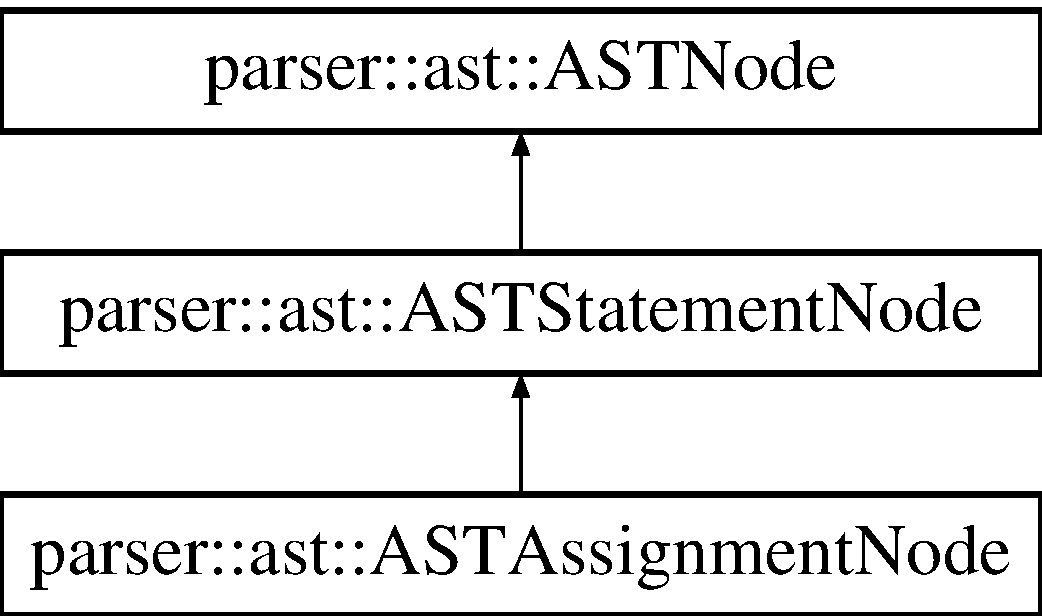
\includegraphics[height=3.000000cm]{d9/de4/classparser_1_1ast_1_1ASTAssignmentNode}
\end{center}
\end{figure}
\subsection*{Public Member Functions}
\begin{DoxyCompactItemize}
\item 
\hyperlink{classparser_1_1ast_1_1ASTAssignmentNode_aa187a542a462035acd30b07555e2c9f8}{A\+S\+T\+Assignment\+Node} (std\+::unique\+\_\+ptr$<$ \hyperlink{classparser_1_1ast_1_1ASTIdentifierNode}{parser\+::ast\+::\+A\+S\+T\+Identifier\+Node} $>$ \hyperlink{classparser_1_1ast_1_1ASTAssignmentNode_adc2b80713ab5ad6a0fa5f173473e505d}{identifier}, std\+::unique\+\_\+ptr$<$ \hyperlink{classparser_1_1ast_1_1ASTExprNode}{A\+S\+T\+Expr\+Node} $>$ expr)
\item 
std\+::unique\+\_\+ptr$<$ \hyperlink{classparser_1_1ast_1_1ASTIdentifierNode}{A\+S\+T\+Identifier\+Node} $>$ \& \hyperlink{classparser_1_1ast_1_1ASTAssignmentNode_aaff40f77ab7db5be4b4c4f354f2e8d7a}{get\+Identifier} ()
\item 
std\+::unique\+\_\+ptr$<$ \hyperlink{classparser_1_1ast_1_1ASTExprNode}{A\+S\+T\+Expr\+Node} $>$ \& \hyperlink{classparser_1_1ast_1_1ASTAssignmentNode_a0610348cf9d4f3302320ebd6598e45e2}{get\+Expr} ()
\item 
Statement\+Type \hyperlink{classparser_1_1ast_1_1ASTAssignmentNode_ad53e33c7aa72d26b67e38699bdac2e32}{get\+Statement\+Type} () override
\item 
void \hyperlink{classparser_1_1ast_1_1ASTAssignmentNode_abfbf5dd90191738f1faea1334fe8480b}{accept} (\hyperlink{classvisitor_1_1Visitor}{visitor\+::\+Visitor} $\ast$visitor) override
\end{DoxyCompactItemize}
\subsection*{Protected Attributes}
\begin{DoxyCompactItemize}
\item 
\mbox{\Hypertarget{classparser_1_1ast_1_1ASTAssignmentNode_adc2b80713ab5ad6a0fa5f173473e505d}\label{classparser_1_1ast_1_1ASTAssignmentNode_adc2b80713ab5ad6a0fa5f173473e505d}} 
std\+::unique\+\_\+ptr$<$ \hyperlink{classparser_1_1ast_1_1ASTIdentifierNode}{A\+S\+T\+Identifier\+Node} $>$ \hyperlink{classparser_1_1ast_1_1ASTAssignmentNode_adc2b80713ab5ad6a0fa5f173473e505d}{identifier}
\begin{DoxyCompactList}\small\item\em The variable\textquotesingle{}s identifier. \end{DoxyCompactList}\item 
\mbox{\Hypertarget{classparser_1_1ast_1_1ASTAssignmentNode_aaf39398fa144912e4be67549d61cff20}\label{classparser_1_1ast_1_1ASTAssignmentNode_aaf39398fa144912e4be67549d61cff20}} 
std\+::unique\+\_\+ptr$<$ \hyperlink{classparser_1_1ast_1_1ASTExprNode}{A\+S\+T\+Expr\+Node} $>$ {\bfseries expr}
\end{DoxyCompactItemize}


\subsection{Detailed Description}
An A\+ST node representing an assignment statement 

\subsection{Constructor \& Destructor Documentation}
\mbox{\Hypertarget{classparser_1_1ast_1_1ASTAssignmentNode_aa187a542a462035acd30b07555e2c9f8}\label{classparser_1_1ast_1_1ASTAssignmentNode_aa187a542a462035acd30b07555e2c9f8}} 
\index{parser\+::ast\+::\+A\+S\+T\+Assignment\+Node@{parser\+::ast\+::\+A\+S\+T\+Assignment\+Node}!A\+S\+T\+Assignment\+Node@{A\+S\+T\+Assignment\+Node}}
\index{A\+S\+T\+Assignment\+Node@{A\+S\+T\+Assignment\+Node}!parser\+::ast\+::\+A\+S\+T\+Assignment\+Node@{parser\+::ast\+::\+A\+S\+T\+Assignment\+Node}}
\subsubsection{\texorpdfstring{A\+S\+T\+Assignment\+Node()}{ASTAssignmentNode()}}
{\footnotesize\ttfamily parser\+::ast\+::\+A\+S\+T\+Assignment\+Node\+::\+A\+S\+T\+Assignment\+Node (\begin{DoxyParamCaption}\item[{std\+::unique\+\_\+ptr$<$ \hyperlink{classparser_1_1ast_1_1ASTIdentifierNode}{parser\+::ast\+::\+A\+S\+T\+Identifier\+Node} $>$}]{identifier,  }\item[{std\+::unique\+\_\+ptr$<$ \hyperlink{classparser_1_1ast_1_1ASTExprNode}{A\+S\+T\+Expr\+Node} $>$}]{expr }\end{DoxyParamCaption})}

The constructor for this class 
\begin{DoxyParams}{Parameters}
{\em identifier} & The identifier of the variable created by this statement \\
\hline
{\em expr} & The expression Node \\
\hline
\end{DoxyParams}


\subsection{Member Function Documentation}
\mbox{\Hypertarget{classparser_1_1ast_1_1ASTAssignmentNode_abfbf5dd90191738f1faea1334fe8480b}\label{classparser_1_1ast_1_1ASTAssignmentNode_abfbf5dd90191738f1faea1334fe8480b}} 
\index{parser\+::ast\+::\+A\+S\+T\+Assignment\+Node@{parser\+::ast\+::\+A\+S\+T\+Assignment\+Node}!accept@{accept}}
\index{accept@{accept}!parser\+::ast\+::\+A\+S\+T\+Assignment\+Node@{parser\+::ast\+::\+A\+S\+T\+Assignment\+Node}}
\subsubsection{\texorpdfstring{accept()}{accept()}}
{\footnotesize\ttfamily void parser\+::ast\+::\+A\+S\+T\+Assignment\+Node\+::accept (\begin{DoxyParamCaption}\item[{\hyperlink{classvisitor_1_1Visitor}{visitor\+::\+Visitor} $\ast$}]{visitor }\end{DoxyParamCaption})\hspace{0.3cm}{\ttfamily [override]}, {\ttfamily [virtual]}}

Accepts a visitor and calls the operation by invoking {\ttfamily visit(this)} 
\begin{DoxyParams}{Parameters}
{\em visitor} & the visitor to accept \\
\hline
\end{DoxyParams}


Implements \hyperlink{classparser_1_1ast_1_1ASTNode_a3ff84fdfdbbc5c39b70b4d04c22e7dc3}{parser\+::ast\+::\+A\+S\+T\+Node}.

\mbox{\Hypertarget{classparser_1_1ast_1_1ASTAssignmentNode_a0610348cf9d4f3302320ebd6598e45e2}\label{classparser_1_1ast_1_1ASTAssignmentNode_a0610348cf9d4f3302320ebd6598e45e2}} 
\index{parser\+::ast\+::\+A\+S\+T\+Assignment\+Node@{parser\+::ast\+::\+A\+S\+T\+Assignment\+Node}!get\+Expr@{get\+Expr}}
\index{get\+Expr@{get\+Expr}!parser\+::ast\+::\+A\+S\+T\+Assignment\+Node@{parser\+::ast\+::\+A\+S\+T\+Assignment\+Node}}
\subsubsection{\texorpdfstring{get\+Expr()}{getExpr()}}
{\footnotesize\ttfamily std\+::unique\+\_\+ptr$<$ \hyperlink{classparser_1_1ast_1_1ASTExprNode}{parser\+::ast\+::\+A\+S\+T\+Expr\+Node} $>$ \& parser\+::ast\+::\+A\+S\+T\+Assignment\+Node\+::get\+Expr (\begin{DoxyParamCaption}{ }\end{DoxyParamCaption})}

\begin{DoxyReturn}{Returns}
A reference to the expression 
\end{DoxyReturn}
\mbox{\Hypertarget{classparser_1_1ast_1_1ASTAssignmentNode_aaff40f77ab7db5be4b4c4f354f2e8d7a}\label{classparser_1_1ast_1_1ASTAssignmentNode_aaff40f77ab7db5be4b4c4f354f2e8d7a}} 
\index{parser\+::ast\+::\+A\+S\+T\+Assignment\+Node@{parser\+::ast\+::\+A\+S\+T\+Assignment\+Node}!get\+Identifier@{get\+Identifier}}
\index{get\+Identifier@{get\+Identifier}!parser\+::ast\+::\+A\+S\+T\+Assignment\+Node@{parser\+::ast\+::\+A\+S\+T\+Assignment\+Node}}
\subsubsection{\texorpdfstring{get\+Identifier()}{getIdentifier()}}
{\footnotesize\ttfamily std\+::unique\+\_\+ptr$<$ \hyperlink{classparser_1_1ast_1_1ASTIdentifierNode}{parser\+::ast\+::\+A\+S\+T\+Identifier\+Node} $>$ \& parser\+::ast\+::\+A\+S\+T\+Assignment\+Node\+::get\+Identifier (\begin{DoxyParamCaption}{ }\end{DoxyParamCaption})}

\begin{DoxyReturn}{Returns}
A reference to the identifier string 
\end{DoxyReturn}
\mbox{\Hypertarget{classparser_1_1ast_1_1ASTAssignmentNode_ad53e33c7aa72d26b67e38699bdac2e32}\label{classparser_1_1ast_1_1ASTAssignmentNode_ad53e33c7aa72d26b67e38699bdac2e32}} 
\index{parser\+::ast\+::\+A\+S\+T\+Assignment\+Node@{parser\+::ast\+::\+A\+S\+T\+Assignment\+Node}!get\+Statement\+Type@{get\+Statement\+Type}}
\index{get\+Statement\+Type@{get\+Statement\+Type}!parser\+::ast\+::\+A\+S\+T\+Assignment\+Node@{parser\+::ast\+::\+A\+S\+T\+Assignment\+Node}}
\subsubsection{\texorpdfstring{get\+Statement\+Type()}{getStatementType()}}
{\footnotesize\ttfamily parser\+::ast\+::\+Statement\+Type parser\+::ast\+::\+A\+S\+T\+Assignment\+Node\+::get\+Statement\+Type (\begin{DoxyParamCaption}{ }\end{DoxyParamCaption})\hspace{0.3cm}{\ttfamily [override]}, {\ttfamily [virtual]}}

Virtual Method to return the statement type \begin{DoxyReturn}{Returns}
The statement type (instead of checking what class it\textquotesingle{}s an instance of) 
\end{DoxyReturn}


Implements \hyperlink{classparser_1_1ast_1_1ASTStatementNode_ac381d35d12f774a1bab0e209c5bfec1f}{parser\+::ast\+::\+A\+S\+T\+Statement\+Node}.



The documentation for this class was generated from the following files\+:\begin{DoxyCompactItemize}
\item 
parser/ast/statement/\hyperlink{ASTAssignmentNode_8h}{A\+S\+T\+Assignment\+Node.\+h}\item 
parser/ast/statement/A\+S\+T\+Assignment\+Node.\+cpp\end{DoxyCompactItemize}

\hypertarget{classparser_1_1ast_1_1ASTBlockStatementNode}{}\section{parser\+:\+:ast\+:\+:A\+S\+T\+Block\+Statement\+Node Class Reference}
\label{classparser_1_1ast_1_1ASTBlockStatementNode}\index{parser\+::ast\+::\+A\+S\+T\+Block\+Statement\+Node@{parser\+::ast\+::\+A\+S\+T\+Block\+Statement\+Node}}
Inheritance diagram for parser\+:\+:ast\+:\+:A\+S\+T\+Block\+Statement\+Node\+:\begin{figure}[H]
\begin{center}
\leavevmode
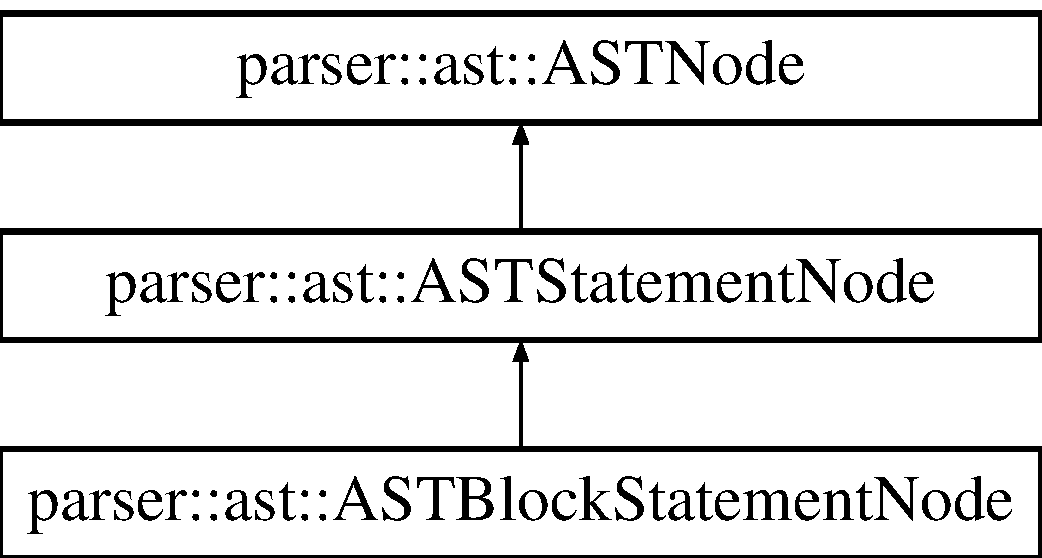
\includegraphics[height=3.000000cm]{d0/d01/classparser_1_1ast_1_1ASTBlockStatementNode}
\end{center}
\end{figure}
\subsection*{Public Member Functions}
\begin{DoxyCompactItemize}
\item 
\mbox{\Hypertarget{classparser_1_1ast_1_1ASTBlockStatementNode_a029059bf25ef46594d1c48bff34c6612}\label{classparser_1_1ast_1_1ASTBlockStatementNode_a029059bf25ef46594d1c48bff34c6612}} 
\hyperlink{classparser_1_1ast_1_1ASTBlockStatementNode_a029059bf25ef46594d1c48bff34c6612}{A\+S\+T\+Block\+Statement\+Node} ()
\begin{DoxyCompactList}\small\item\em Default constructor, with an empty block. \end{DoxyCompactList}\item 
\hyperlink{classparser_1_1ast_1_1ASTBlockStatementNode_a69b3e477b9945bb1567560f2951c9bcd}{A\+S\+T\+Block\+Statement\+Node} (std\+::vector$<$ std\+::unique\+\_\+ptr$<$ \hyperlink{classparser_1_1ast_1_1ASTStatementNode}{A\+S\+T\+Statement\+Node} $>$$>$ \&contents)
\item 
Statement\+Type \hyperlink{classparser_1_1ast_1_1ASTBlockStatementNode_aec80a6d582f0b9691dbd33d0d5ecb975}{get\+Statement\+Type} () override
\item 
void \hyperlink{classparser_1_1ast_1_1ASTBlockStatementNode_ae0e7e04747661471aade0c1509c37422}{accept} (\hyperlink{classvisitor_1_1Visitor}{visitor\+::\+Visitor} $\ast$visitor) override
\end{DoxyCompactItemize}
\subsection*{Public Attributes}
\begin{DoxyCompactItemize}
\item 
std\+::vector$<$ std\+::unique\+\_\+ptr$<$ \hyperlink{classparser_1_1ast_1_1ASTStatementNode}{A\+S\+T\+Statement\+Node} $>$ $>$ \hyperlink{classparser_1_1ast_1_1ASTBlockStatementNode_abbd8aa518677035cba32a20a4d7135ac}{block\+Contents}
\begin{DoxyCompactList}\small\item\em The contents of this block. \end{DoxyCompactList}\end{DoxyCompactItemize}


\subsection{Constructor \& Destructor Documentation}
\mbox{\Hypertarget{classparser_1_1ast_1_1ASTBlockStatementNode_a69b3e477b9945bb1567560f2951c9bcd}\label{classparser_1_1ast_1_1ASTBlockStatementNode_a69b3e477b9945bb1567560f2951c9bcd}} 
\index{parser\+::ast\+::\+A\+S\+T\+Block\+Statement\+Node@{parser\+::ast\+::\+A\+S\+T\+Block\+Statement\+Node}!A\+S\+T\+Block\+Statement\+Node@{A\+S\+T\+Block\+Statement\+Node}}
\index{A\+S\+T\+Block\+Statement\+Node@{A\+S\+T\+Block\+Statement\+Node}!parser\+::ast\+::\+A\+S\+T\+Block\+Statement\+Node@{parser\+::ast\+::\+A\+S\+T\+Block\+Statement\+Node}}
\subsubsection{\texorpdfstring{A\+S\+T\+Block\+Statement\+Node()}{ASTBlockStatementNode()}}
{\footnotesize\ttfamily parser\+::ast\+::\+A\+S\+T\+Block\+Statement\+Node\+::\+A\+S\+T\+Block\+Statement\+Node (\begin{DoxyParamCaption}\item[{std\+::vector$<$ std\+::unique\+\_\+ptr$<$ \hyperlink{classparser_1_1ast_1_1ASTStatementNode}{A\+S\+T\+Statement\+Node} $>$$>$ \&}]{contents }\end{DoxyParamCaption})}

Constructor for known block 
\begin{DoxyParams}{Parameters}
{\em block\+Contents} & The statements in this block. \\
\hline
\end{DoxyParams}


\subsection{Member Function Documentation}
\mbox{\Hypertarget{classparser_1_1ast_1_1ASTBlockStatementNode_ae0e7e04747661471aade0c1509c37422}\label{classparser_1_1ast_1_1ASTBlockStatementNode_ae0e7e04747661471aade0c1509c37422}} 
\index{parser\+::ast\+::\+A\+S\+T\+Block\+Statement\+Node@{parser\+::ast\+::\+A\+S\+T\+Block\+Statement\+Node}!accept@{accept}}
\index{accept@{accept}!parser\+::ast\+::\+A\+S\+T\+Block\+Statement\+Node@{parser\+::ast\+::\+A\+S\+T\+Block\+Statement\+Node}}
\subsubsection{\texorpdfstring{accept()}{accept()}}
{\footnotesize\ttfamily void parser\+::ast\+::\+A\+S\+T\+Block\+Statement\+Node\+::accept (\begin{DoxyParamCaption}\item[{\hyperlink{classvisitor_1_1Visitor}{visitor\+::\+Visitor} $\ast$}]{visitor }\end{DoxyParamCaption})\hspace{0.3cm}{\ttfamily [override]}, {\ttfamily [virtual]}}

Accepts a visitor and calls the operation by invoking {\ttfamily visit(this)} 
\begin{DoxyParams}{Parameters}
{\em visitor} & the visitor to accept \\
\hline
\end{DoxyParams}


Implements \hyperlink{classparser_1_1ast_1_1ASTNode_a3ff84fdfdbbc5c39b70b4d04c22e7dc3}{parser\+::ast\+::\+A\+S\+T\+Node}.

\mbox{\Hypertarget{classparser_1_1ast_1_1ASTBlockStatementNode_aec80a6d582f0b9691dbd33d0d5ecb975}\label{classparser_1_1ast_1_1ASTBlockStatementNode_aec80a6d582f0b9691dbd33d0d5ecb975}} 
\index{parser\+::ast\+::\+A\+S\+T\+Block\+Statement\+Node@{parser\+::ast\+::\+A\+S\+T\+Block\+Statement\+Node}!get\+Statement\+Type@{get\+Statement\+Type}}
\index{get\+Statement\+Type@{get\+Statement\+Type}!parser\+::ast\+::\+A\+S\+T\+Block\+Statement\+Node@{parser\+::ast\+::\+A\+S\+T\+Block\+Statement\+Node}}
\subsubsection{\texorpdfstring{get\+Statement\+Type()}{getStatementType()}}
{\footnotesize\ttfamily parser\+::ast\+::\+Statement\+Type parser\+::ast\+::\+A\+S\+T\+Block\+Statement\+Node\+::get\+Statement\+Type (\begin{DoxyParamCaption}{ }\end{DoxyParamCaption})\hspace{0.3cm}{\ttfamily [override]}, {\ttfamily [virtual]}}

Virtual Method to return the statement type \begin{DoxyReturn}{Returns}
The statement type (instead of checking what class it\textquotesingle{}s an instance of) 
\end{DoxyReturn}


Implements \hyperlink{classparser_1_1ast_1_1ASTStatementNode_ac381d35d12f774a1bab0e209c5bfec1f}{parser\+::ast\+::\+A\+S\+T\+Statement\+Node}.



\subsection{Member Data Documentation}
\mbox{\Hypertarget{classparser_1_1ast_1_1ASTBlockStatementNode_abbd8aa518677035cba32a20a4d7135ac}\label{classparser_1_1ast_1_1ASTBlockStatementNode_abbd8aa518677035cba32a20a4d7135ac}} 
\index{parser\+::ast\+::\+A\+S\+T\+Block\+Statement\+Node@{parser\+::ast\+::\+A\+S\+T\+Block\+Statement\+Node}!block\+Contents@{block\+Contents}}
\index{block\+Contents@{block\+Contents}!parser\+::ast\+::\+A\+S\+T\+Block\+Statement\+Node@{parser\+::ast\+::\+A\+S\+T\+Block\+Statement\+Node}}
\subsubsection{\texorpdfstring{block\+Contents}{blockContents}}
{\footnotesize\ttfamily std\+::vector$<$std\+::unique\+\_\+ptr$<$\hyperlink{classparser_1_1ast_1_1ASTStatementNode}{A\+S\+T\+Statement\+Node}$>$ $>$ parser\+::ast\+::\+A\+S\+T\+Block\+Statement\+Node\+::block\+Contents}



The contents of this block. 

This has a public visibility since \hyperlink{classparser_1_1ast_1_1ASTBlockStatementNode}{A\+S\+T\+Block\+Statement\+Node} is really a wrapper. A {\ttfamily typedef} wasn\textquotesingle{}t used due to the inheritance scheme for this class. 

The documentation for this class was generated from the following files\+:\begin{DoxyCompactItemize}
\item 
parser/ast/statement/\hyperlink{ASTBlockStatementNode_8h}{A\+S\+T\+Block\+Statement\+Node.\+h}\item 
parser/ast/statement/A\+S\+T\+Block\+Statement\+Node.\+cpp\end{DoxyCompactItemize}

\hypertarget{classparser_1_1ast_1_1ASTExprNode}{}\section{parser\+:\+:ast\+:\+:A\+S\+T\+Expr\+Node Class Reference}
\label{classparser_1_1ast_1_1ASTExprNode}\index{parser\+::ast\+::\+A\+S\+T\+Expr\+Node@{parser\+::ast\+::\+A\+S\+T\+Expr\+Node}}
Inheritance diagram for parser\+:\+:ast\+:\+:A\+S\+T\+Expr\+Node\+:\begin{figure}[H]
\begin{center}
\leavevmode
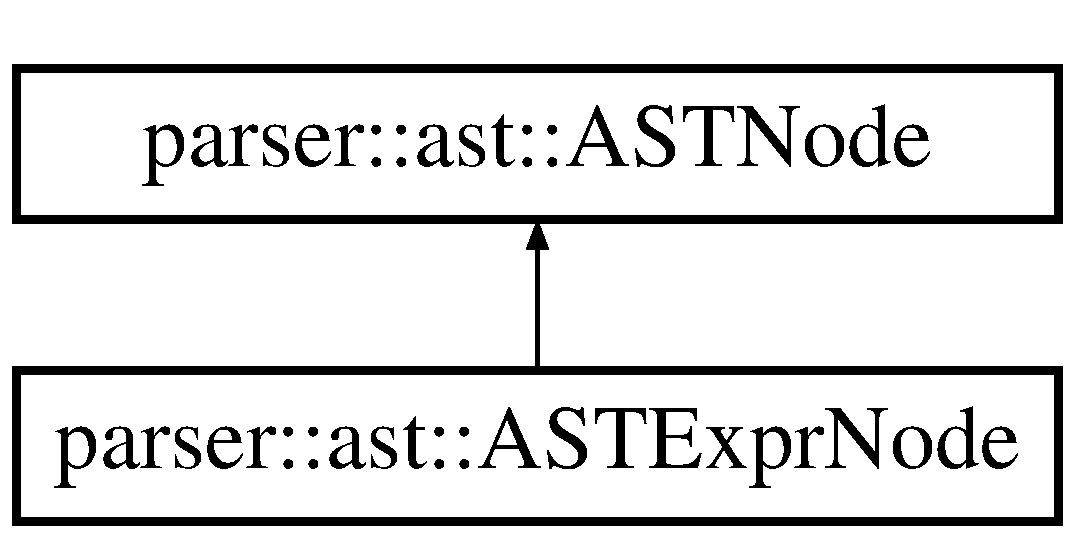
\includegraphics[height=2.000000cm]{db/dc8/classparser_1_1ast_1_1ASTExprNode}
\end{center}
\end{figure}
\subsection*{Public Member Functions}
\begin{DoxyCompactItemize}
\item 
\hyperlink{classparser_1_1ast_1_1ASTExprNode_a591850e9f50fcbb6f8d97f3a40a3a2ba}{A\+S\+T\+Expr\+Node} (std\+::unique\+\_\+ptr$<$ \hyperlink{classparser_1_1ast_1_1ASTSimpleExprNode}{A\+S\+T\+Simple\+Expr\+Node} $>$ \hyperlink{classparser_1_1ast_1_1ASTExprNode_aa7250732754b829ca100d4ce35a021b0}{left}, \hyperlink{ASTExprNode_8h_ade5793e91a548ec55c1a8e776984297a}{Rel\+Op\+Type} \hyperlink{classparser_1_1ast_1_1ASTExprNode_a45fa00b5859baeb11b6976b145b5966e}{relational\+Operator}, std\+::unique\+\_\+ptr$<$ \hyperlink{classparser_1_1ast_1_1ASTSimpleExprNode}{A\+S\+T\+Simple\+Expr\+Node} $>$ \hyperlink{classparser_1_1ast_1_1ASTExprNode_a26f40099c4e3848ba0ed00388d507d72}{right})
\item 
\hyperlink{classparser_1_1ast_1_1ASTExprNode_a1716bec11dcf773ef5090c13fa7e8020}{A\+S\+T\+Expr\+Node} (std\+::unique\+\_\+ptr$<$ \hyperlink{classparser_1_1ast_1_1ASTSimpleExprNode}{A\+S\+T\+Simple\+Expr\+Node} $>$ \hyperlink{classparser_1_1ast_1_1ASTExprNode_aa7250732754b829ca100d4ce35a021b0}{left})
\item 
const std\+::unique\+\_\+ptr$<$ \hyperlink{classparser_1_1ast_1_1ASTSimpleExprNode}{A\+S\+T\+Simple\+Expr\+Node} $>$ \& \hyperlink{classparser_1_1ast_1_1ASTExprNode_a19ec44a2b2a38635c6e9cf7fa398fb76}{get\+Left} () const
\item 
\hyperlink{ASTExprNode_8h_ade5793e91a548ec55c1a8e776984297a}{Rel\+Op\+Type} \hyperlink{classparser_1_1ast_1_1ASTExprNode_af4efd2fc330c3fa5da59334b9db9b104}{get\+Relational\+Operator} () const
\item 
const std\+::unique\+\_\+ptr$<$ \hyperlink{classparser_1_1ast_1_1ASTSimpleExprNode}{A\+S\+T\+Simple\+Expr\+Node} $>$ \& \hyperlink{classparser_1_1ast_1_1ASTExprNode_a23aad8e7397e524848446e9bdcdc4141}{get\+Right} () const
\item 
const std\+::string \hyperlink{classparser_1_1ast_1_1ASTExprNode_a3e781b545bb07447252f265a06f94b93}{get\+Rel\+Op\+String} () const
\item 
void \hyperlink{classparser_1_1ast_1_1ASTExprNode_a3eea258af04a74930acc0c9fb6aade77}{accept} (\hyperlink{classvisitor_1_1Visitor}{visitor\+::\+Visitor} $\ast$visitor) override
\end{DoxyCompactItemize}
\subsection*{Protected Attributes}
\begin{DoxyCompactItemize}
\item 
\mbox{\Hypertarget{classparser_1_1ast_1_1ASTExprNode_aa7250732754b829ca100d4ce35a021b0}\label{classparser_1_1ast_1_1ASTExprNode_aa7250732754b829ca100d4ce35a021b0}} 
std\+::unique\+\_\+ptr$<$ \hyperlink{classparser_1_1ast_1_1ASTSimpleExprNode}{A\+S\+T\+Simple\+Expr\+Node} $>$ \hyperlink{classparser_1_1ast_1_1ASTExprNode_aa7250732754b829ca100d4ce35a021b0}{left}
\begin{DoxyCompactList}\small\item\em The Simple Expression on the left hand side. This is mandatory. \end{DoxyCompactList}\item 
\mbox{\Hypertarget{classparser_1_1ast_1_1ASTExprNode_a45fa00b5859baeb11b6976b145b5966e}\label{classparser_1_1ast_1_1ASTExprNode_a45fa00b5859baeb11b6976b145b5966e}} 
\hyperlink{ASTExprNode_8h_ade5793e91a548ec55c1a8e776984297a}{Rel\+Op\+Type} \hyperlink{classparser_1_1ast_1_1ASTExprNode_a45fa00b5859baeb11b6976b145b5966e}{relational\+Operator}
\begin{DoxyCompactList}\small\item\em The Relational operator between the 2 simple expressions. Mandatory if the right hand side is not null. \end{DoxyCompactList}\item 
\mbox{\Hypertarget{classparser_1_1ast_1_1ASTExprNode_a26f40099c4e3848ba0ed00388d507d72}\label{classparser_1_1ast_1_1ASTExprNode_a26f40099c4e3848ba0ed00388d507d72}} 
std\+::unique\+\_\+ptr$<$ \hyperlink{classparser_1_1ast_1_1ASTSimpleExprNode}{A\+S\+T\+Simple\+Expr\+Node} $>$ \hyperlink{classparser_1_1ast_1_1ASTExprNode_a26f40099c4e3848ba0ed00388d507d72}{right}
\begin{DoxyCompactList}\small\item\em The Simple Expression on the right hand side. Optional. \end{DoxyCompactList}\end{DoxyCompactItemize}


\subsection{Constructor \& Destructor Documentation}
\mbox{\Hypertarget{classparser_1_1ast_1_1ASTExprNode_a591850e9f50fcbb6f8d97f3a40a3a2ba}\label{classparser_1_1ast_1_1ASTExprNode_a591850e9f50fcbb6f8d97f3a40a3a2ba}} 
\index{parser\+::ast\+::\+A\+S\+T\+Expr\+Node@{parser\+::ast\+::\+A\+S\+T\+Expr\+Node}!A\+S\+T\+Expr\+Node@{A\+S\+T\+Expr\+Node}}
\index{A\+S\+T\+Expr\+Node@{A\+S\+T\+Expr\+Node}!parser\+::ast\+::\+A\+S\+T\+Expr\+Node@{parser\+::ast\+::\+A\+S\+T\+Expr\+Node}}
\subsubsection{\texorpdfstring{A\+S\+T\+Expr\+Node()}{ASTExprNode()}\hspace{0.1cm}{\footnotesize\ttfamily [1/2]}}
{\footnotesize\ttfamily parser\+::ast\+::\+A\+S\+T\+Expr\+Node\+::\+A\+S\+T\+Expr\+Node (\begin{DoxyParamCaption}\item[{std\+::unique\+\_\+ptr$<$ \hyperlink{classparser_1_1ast_1_1ASTSimpleExprNode}{A\+S\+T\+Simple\+Expr\+Node} $>$}]{left,  }\item[{\hyperlink{ASTExprNode_8h_ade5793e91a548ec55c1a8e776984297a}{Rel\+Op\+Type}}]{relational\+Operator,  }\item[{std\+::unique\+\_\+ptr$<$ \hyperlink{classparser_1_1ast_1_1ASTSimpleExprNode}{A\+S\+T\+Simple\+Expr\+Node} $>$}]{right }\end{DoxyParamCaption})}

Constructor for an expression with both sides of the relation operator 
\begin{DoxyParams}{Parameters}
{\em left} & The left hand side of this expression \\
\hline
{\em relational\+Operator} & The relational operator applied to this \\
\hline
{\em right} & The right hand side of this expression \\
\hline
\end{DoxyParams}
\mbox{\Hypertarget{classparser_1_1ast_1_1ASTExprNode_a1716bec11dcf773ef5090c13fa7e8020}\label{classparser_1_1ast_1_1ASTExprNode_a1716bec11dcf773ef5090c13fa7e8020}} 
\index{parser\+::ast\+::\+A\+S\+T\+Expr\+Node@{parser\+::ast\+::\+A\+S\+T\+Expr\+Node}!A\+S\+T\+Expr\+Node@{A\+S\+T\+Expr\+Node}}
\index{A\+S\+T\+Expr\+Node@{A\+S\+T\+Expr\+Node}!parser\+::ast\+::\+A\+S\+T\+Expr\+Node@{parser\+::ast\+::\+A\+S\+T\+Expr\+Node}}
\subsubsection{\texorpdfstring{A\+S\+T\+Expr\+Node()}{ASTExprNode()}\hspace{0.1cm}{\footnotesize\ttfamily [2/2]}}
{\footnotesize\ttfamily parser\+::ast\+::\+A\+S\+T\+Expr\+Node\+::\+A\+S\+T\+Expr\+Node (\begin{DoxyParamCaption}\item[{std\+::unique\+\_\+ptr$<$ \hyperlink{classparser_1_1ast_1_1ASTSimpleExprNode}{A\+S\+T\+Simple\+Expr\+Node} $>$}]{left }\end{DoxyParamCaption})}

Constructor for when an expression does not have a relational operator 
\begin{DoxyParams}{Parameters}
{\em left} & The simple expression this expression is made of. \\
\hline
\end{DoxyParams}


\subsection{Member Function Documentation}
\mbox{\Hypertarget{classparser_1_1ast_1_1ASTExprNode_a3eea258af04a74930acc0c9fb6aade77}\label{classparser_1_1ast_1_1ASTExprNode_a3eea258af04a74930acc0c9fb6aade77}} 
\index{parser\+::ast\+::\+A\+S\+T\+Expr\+Node@{parser\+::ast\+::\+A\+S\+T\+Expr\+Node}!accept@{accept}}
\index{accept@{accept}!parser\+::ast\+::\+A\+S\+T\+Expr\+Node@{parser\+::ast\+::\+A\+S\+T\+Expr\+Node}}
\subsubsection{\texorpdfstring{accept()}{accept()}}
{\footnotesize\ttfamily void parser\+::ast\+::\+A\+S\+T\+Expr\+Node\+::accept (\begin{DoxyParamCaption}\item[{\hyperlink{classvisitor_1_1Visitor}{visitor\+::\+Visitor} $\ast$}]{visitor }\end{DoxyParamCaption})\hspace{0.3cm}{\ttfamily [override]}, {\ttfamily [virtual]}}

Accepts a visitor and calls the operation by invoking {\ttfamily visit(this)} 
\begin{DoxyParams}{Parameters}
{\em visitor} & the visitor to accept \\
\hline
\end{DoxyParams}


Implements \hyperlink{classparser_1_1ast_1_1ASTNode_a3ff84fdfdbbc5c39b70b4d04c22e7dc3}{parser\+::ast\+::\+A\+S\+T\+Node}.

\mbox{\Hypertarget{classparser_1_1ast_1_1ASTExprNode_a19ec44a2b2a38635c6e9cf7fa398fb76}\label{classparser_1_1ast_1_1ASTExprNode_a19ec44a2b2a38635c6e9cf7fa398fb76}} 
\index{parser\+::ast\+::\+A\+S\+T\+Expr\+Node@{parser\+::ast\+::\+A\+S\+T\+Expr\+Node}!get\+Left@{get\+Left}}
\index{get\+Left@{get\+Left}!parser\+::ast\+::\+A\+S\+T\+Expr\+Node@{parser\+::ast\+::\+A\+S\+T\+Expr\+Node}}
\subsubsection{\texorpdfstring{get\+Left()}{getLeft()}}
{\footnotesize\ttfamily const std\+::unique\+\_\+ptr$<$ \hyperlink{classparser_1_1ast_1_1ASTSimpleExprNode}{parser\+::ast\+::\+A\+S\+T\+Simple\+Expr\+Node} $>$ \& parser\+::ast\+::\+A\+S\+T\+Expr\+Node\+::get\+Left (\begin{DoxyParamCaption}{ }\end{DoxyParamCaption}) const}

\begin{DoxyReturn}{Returns}
The left hand side of this expression 
\end{DoxyReturn}
\mbox{\Hypertarget{classparser_1_1ast_1_1ASTExprNode_af4efd2fc330c3fa5da59334b9db9b104}\label{classparser_1_1ast_1_1ASTExprNode_af4efd2fc330c3fa5da59334b9db9b104}} 
\index{parser\+::ast\+::\+A\+S\+T\+Expr\+Node@{parser\+::ast\+::\+A\+S\+T\+Expr\+Node}!get\+Relational\+Operator@{get\+Relational\+Operator}}
\index{get\+Relational\+Operator@{get\+Relational\+Operator}!parser\+::ast\+::\+A\+S\+T\+Expr\+Node@{parser\+::ast\+::\+A\+S\+T\+Expr\+Node}}
\subsubsection{\texorpdfstring{get\+Relational\+Operator()}{getRelationalOperator()}}
{\footnotesize\ttfamily \hyperlink{ASTExprNode_8h_ade5793e91a548ec55c1a8e776984297a}{parser\+::ast\+::\+Rel\+Op\+Type} parser\+::ast\+::\+A\+S\+T\+Expr\+Node\+::get\+Relational\+Operator (\begin{DoxyParamCaption}{ }\end{DoxyParamCaption}) const}

\begin{DoxyReturn}{Returns}
The relation operator used in this expression N\+U\+LL if there is no right hand side 
\end{DoxyReturn}
\mbox{\Hypertarget{classparser_1_1ast_1_1ASTExprNode_a3e781b545bb07447252f265a06f94b93}\label{classparser_1_1ast_1_1ASTExprNode_a3e781b545bb07447252f265a06f94b93}} 
\index{parser\+::ast\+::\+A\+S\+T\+Expr\+Node@{parser\+::ast\+::\+A\+S\+T\+Expr\+Node}!get\+Rel\+Op\+String@{get\+Rel\+Op\+String}}
\index{get\+Rel\+Op\+String@{get\+Rel\+Op\+String}!parser\+::ast\+::\+A\+S\+T\+Expr\+Node@{parser\+::ast\+::\+A\+S\+T\+Expr\+Node}}
\subsubsection{\texorpdfstring{get\+Rel\+Op\+String()}{getRelOpString()}}
{\footnotesize\ttfamily const std\+::string parser\+::ast\+::\+A\+S\+T\+Expr\+Node\+::get\+Rel\+Op\+String (\begin{DoxyParamCaption}{ }\end{DoxyParamCaption}) const}


\begin{DoxyParams}{Parameters}
{\em The} & relation operator to convert to a string \\
\hline
\end{DoxyParams}
\begin{DoxyReturn}{Returns}
The string for the relational operator 
\end{DoxyReturn}
\mbox{\Hypertarget{classparser_1_1ast_1_1ASTExprNode_a23aad8e7397e524848446e9bdcdc4141}\label{classparser_1_1ast_1_1ASTExprNode_a23aad8e7397e524848446e9bdcdc4141}} 
\index{parser\+::ast\+::\+A\+S\+T\+Expr\+Node@{parser\+::ast\+::\+A\+S\+T\+Expr\+Node}!get\+Right@{get\+Right}}
\index{get\+Right@{get\+Right}!parser\+::ast\+::\+A\+S\+T\+Expr\+Node@{parser\+::ast\+::\+A\+S\+T\+Expr\+Node}}
\subsubsection{\texorpdfstring{get\+Right()}{getRight()}}
{\footnotesize\ttfamily const std\+::unique\+\_\+ptr$<$ \hyperlink{classparser_1_1ast_1_1ASTSimpleExprNode}{parser\+::ast\+::\+A\+S\+T\+Simple\+Expr\+Node} $>$ \& parser\+::ast\+::\+A\+S\+T\+Expr\+Node\+::get\+Right (\begin{DoxyParamCaption}{ }\end{DoxyParamCaption}) const}

\begin{DoxyReturn}{Returns}
A pointer to the right hand side of this expression A pointer is returned as this is optional. 
\end{DoxyReturn}


The documentation for this class was generated from the following files\+:\begin{DoxyCompactItemize}
\item 
parser/ast/\hyperlink{ASTExprNode_8h}{A\+S\+T\+Expr\+Node.\+h}\item 
parser/ast/A\+S\+T\+Expr\+Node.\+cpp\end{DoxyCompactItemize}

\hypertarget{classparser_1_1ast_1_1ASTFactorNode}{}\section{parser\+:\+:ast\+:\+:A\+S\+T\+Factor\+Node Class Reference}
\label{classparser_1_1ast_1_1ASTFactorNode}\index{parser\+::ast\+::\+A\+S\+T\+Factor\+Node@{parser\+::ast\+::\+A\+S\+T\+Factor\+Node}}


{\ttfamily \#include $<$A\+S\+T\+Factor\+Node.\+h$>$}

Inheritance diagram for parser\+:\+:ast\+:\+:A\+S\+T\+Factor\+Node\+:\begin{figure}[H]
\begin{center}
\leavevmode
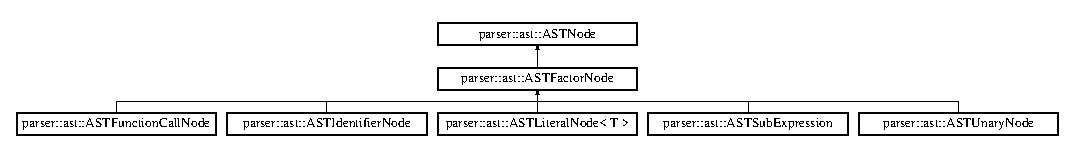
\includegraphics[height=1.600000cm]{d4/dc3/classparser_1_1ast_1_1ASTFactorNode}
\end{center}
\end{figure}
\subsection*{Public Member Functions}
\begin{DoxyCompactItemize}
\item 
virtual \hyperlink{ASTFactorNode_8h_afbe2fcc03ef15b74a0c1ed1cda7ab0e8}{Factor\+Type} \hyperlink{classparser_1_1ast_1_1ASTFactorNode_a13eea7f949c0055dea0a9d7b715f16a8}{get\+Factor\+Type} ()=0
\end{DoxyCompactItemize}


\subsection{Detailed Description}
Class representing an abstract factor node in the A\+ST 

\subsection{Member Function Documentation}
\mbox{\Hypertarget{classparser_1_1ast_1_1ASTFactorNode_a13eea7f949c0055dea0a9d7b715f16a8}\label{classparser_1_1ast_1_1ASTFactorNode_a13eea7f949c0055dea0a9d7b715f16a8}} 
\index{parser\+::ast\+::\+A\+S\+T\+Factor\+Node@{parser\+::ast\+::\+A\+S\+T\+Factor\+Node}!get\+Factor\+Type@{get\+Factor\+Type}}
\index{get\+Factor\+Type@{get\+Factor\+Type}!parser\+::ast\+::\+A\+S\+T\+Factor\+Node@{parser\+::ast\+::\+A\+S\+T\+Factor\+Node}}
\subsubsection{\texorpdfstring{get\+Factor\+Type()}{getFactorType()}}
{\footnotesize\ttfamily virtual \hyperlink{ASTFactorNode_8h_afbe2fcc03ef15b74a0c1ed1cda7ab0e8}{Factor\+Type} parser\+::ast\+::\+A\+S\+T\+Factor\+Node\+::get\+Factor\+Type (\begin{DoxyParamCaption}{ }\end{DoxyParamCaption})\hspace{0.3cm}{\ttfamily [pure virtual]}}

\begin{DoxyReturn}{Returns}
The type of factor this is. Use instead of checking the class type. 
\end{DoxyReturn}


Implemented in \hyperlink{classparser_1_1ast_1_1ASTUnaryNode_a1056ebc5c34b6f3b0a5485f4cd5ba3c0}{parser\+::ast\+::\+A\+S\+T\+Unary\+Node}, \hyperlink{classparser_1_1ast_1_1ASTLiteralNode_a08efdbff5f7b0a0b7623ad964a6e4a9f}{parser\+::ast\+::\+A\+S\+T\+Literal\+Node$<$ T $>$}, \hyperlink{classparser_1_1ast_1_1ASTSubExpression_a0a7ade91b1cce64eacfb9b5f6167db3f}{parser\+::ast\+::\+A\+S\+T\+Sub\+Expression}, \hyperlink{classparser_1_1ast_1_1ASTIdentifierNode_a7b759817af29784741596a4387b6547f}{parser\+::ast\+::\+A\+S\+T\+Identifier\+Node}, and \hyperlink{classparser_1_1ast_1_1ASTFunctionCallNode_a1c40c8e98284fd4389b34da161e8b39a}{parser\+::ast\+::\+A\+S\+T\+Function\+Call\+Node}.



The documentation for this class was generated from the following file\+:\begin{DoxyCompactItemize}
\item 
parser/ast/expression/\hyperlink{ASTFactorNode_8h}{A\+S\+T\+Factor\+Node.\+h}\end{DoxyCompactItemize}

\hypertarget{classparser_1_1ast_1_1ASTFunctionCallNode}{}\section{parser\+:\+:ast\+:\+:A\+S\+T\+Function\+Call\+Node Class Reference}
\label{classparser_1_1ast_1_1ASTFunctionCallNode}\index{parser\+::ast\+::\+A\+S\+T\+Function\+Call\+Node@{parser\+::ast\+::\+A\+S\+T\+Function\+Call\+Node}}
Inheritance diagram for parser\+:\+:ast\+:\+:A\+S\+T\+Function\+Call\+Node\+:\begin{figure}[H]
\begin{center}
\leavevmode
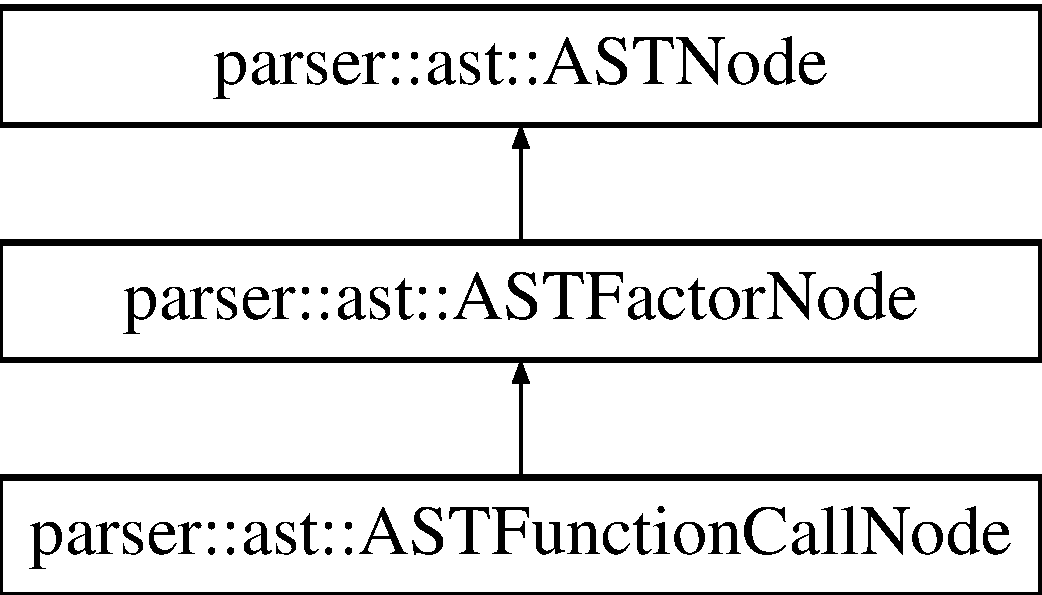
\includegraphics[height=3.000000cm]{de/d41/classparser_1_1ast_1_1ASTFunctionCallNode}
\end{center}
\end{figure}
\subsection*{Public Member Functions}
\begin{DoxyCompactItemize}
\item 
\mbox{\Hypertarget{classparser_1_1ast_1_1ASTFunctionCallNode_a671c8a09cc22abb8a34f1f3945bc9360}\label{classparser_1_1ast_1_1ASTFunctionCallNode_a671c8a09cc22abb8a34f1f3945bc9360}} 
{\bfseries A\+S\+T\+Function\+Call\+Node} (std\+::unique\+\_\+ptr$<$ \hyperlink{classparser_1_1ast_1_1ASTIdentifierNode}{A\+S\+T\+Identifier\+Node} $>$ \hyperlink{classparser_1_1ast_1_1ASTFunctionCallNode_a77b1b97d1a948b8f48e2b67ccedda22b}{identifier}, std\+::vector$<$ std\+::unique\+\_\+ptr$<$ \hyperlink{classparser_1_1ast_1_1ASTExprNode}{A\+S\+T\+Expr\+Node} $>$$>$ \&\hyperlink{classparser_1_1ast_1_1ASTFunctionCallNode_abb9d7f3a34dc376b885b321dc0cef0d3}{actual\+Params})
\item 
\mbox{\Hypertarget{classparser_1_1ast_1_1ASTFunctionCallNode_aefa1003a3388b80e2144ec8fd7161b18}\label{classparser_1_1ast_1_1ASTFunctionCallNode_aefa1003a3388b80e2144ec8fd7161b18}} 
{\bfseries A\+S\+T\+Function\+Call\+Node} (std\+::unique\+\_\+ptr$<$ \hyperlink{classparser_1_1ast_1_1ASTIdentifierNode}{A\+S\+T\+Identifier\+Node} $>$ \hyperlink{classparser_1_1ast_1_1ASTFunctionCallNode_a77b1b97d1a948b8f48e2b67ccedda22b}{identifier})
\item 
\hyperlink{ASTFactorNode_8h_afbe2fcc03ef15b74a0c1ed1cda7ab0e8}{Factor\+Type} \hyperlink{classparser_1_1ast_1_1ASTFunctionCallNode_a1c40c8e98284fd4389b34da161e8b39a}{get\+Factor\+Type} () override
\item 
\mbox{\Hypertarget{classparser_1_1ast_1_1ASTFunctionCallNode_ad5ef8ae75a99a84683f5314bab355dc4}\label{classparser_1_1ast_1_1ASTFunctionCallNode_ad5ef8ae75a99a84683f5314bab355dc4}} 
std\+::unique\+\_\+ptr$<$ \hyperlink{classparser_1_1ast_1_1ASTIdentifierNode}{A\+S\+T\+Identifier\+Node} $>$ \& {\bfseries get\+Identifier} ()
\item 
\mbox{\Hypertarget{classparser_1_1ast_1_1ASTFunctionCallNode_a550822b2c150f4b37d7780428c565e2c}\label{classparser_1_1ast_1_1ASTFunctionCallNode_a550822b2c150f4b37d7780428c565e2c}} 
std\+::vector$<$ std\+::unique\+\_\+ptr$<$ \hyperlink{classparser_1_1ast_1_1ASTExprNode}{A\+S\+T\+Expr\+Node} $>$ $>$ \& {\bfseries get\+Actual\+Params} ()
\item 
void \hyperlink{classparser_1_1ast_1_1ASTFunctionCallNode_ad7ff48d8398744b1211a6da0399a197b}{accept} (\hyperlink{classvisitor_1_1Visitor}{visitor\+::\+Visitor} $\ast$visitor) override
\end{DoxyCompactItemize}
\subsection*{Protected Attributes}
\begin{DoxyCompactItemize}
\item 
\mbox{\Hypertarget{classparser_1_1ast_1_1ASTFunctionCallNode_a77b1b97d1a948b8f48e2b67ccedda22b}\label{classparser_1_1ast_1_1ASTFunctionCallNode_a77b1b97d1a948b8f48e2b67ccedda22b}} 
std\+::unique\+\_\+ptr$<$ \hyperlink{classparser_1_1ast_1_1ASTIdentifierNode}{A\+S\+T\+Identifier\+Node} $>$ \hyperlink{classparser_1_1ast_1_1ASTFunctionCallNode_a77b1b97d1a948b8f48e2b67ccedda22b}{identifier}
\begin{DoxyCompactList}\small\item\em The function name. \end{DoxyCompactList}\item 
\mbox{\Hypertarget{classparser_1_1ast_1_1ASTFunctionCallNode_abb9d7f3a34dc376b885b321dc0cef0d3}\label{classparser_1_1ast_1_1ASTFunctionCallNode_abb9d7f3a34dc376b885b321dc0cef0d3}} 
std\+::vector$<$ std\+::unique\+\_\+ptr$<$ \hyperlink{classparser_1_1ast_1_1ASTExprNode}{A\+S\+T\+Expr\+Node} $>$ $>$ \hyperlink{classparser_1_1ast_1_1ASTFunctionCallNode_abb9d7f3a34dc376b885b321dc0cef0d3}{actual\+Params}
\begin{DoxyCompactList}\small\item\em The parameters to be passed. \end{DoxyCompactList}\end{DoxyCompactItemize}


\subsection{Member Function Documentation}
\mbox{\Hypertarget{classparser_1_1ast_1_1ASTFunctionCallNode_ad7ff48d8398744b1211a6da0399a197b}\label{classparser_1_1ast_1_1ASTFunctionCallNode_ad7ff48d8398744b1211a6da0399a197b}} 
\index{parser\+::ast\+::\+A\+S\+T\+Function\+Call\+Node@{parser\+::ast\+::\+A\+S\+T\+Function\+Call\+Node}!accept@{accept}}
\index{accept@{accept}!parser\+::ast\+::\+A\+S\+T\+Function\+Call\+Node@{parser\+::ast\+::\+A\+S\+T\+Function\+Call\+Node}}
\subsubsection{\texorpdfstring{accept()}{accept()}}
{\footnotesize\ttfamily void parser\+::ast\+::\+A\+S\+T\+Function\+Call\+Node\+::accept (\begin{DoxyParamCaption}\item[{\hyperlink{classvisitor_1_1Visitor}{visitor\+::\+Visitor} $\ast$}]{visitor }\end{DoxyParamCaption})\hspace{0.3cm}{\ttfamily [override]}, {\ttfamily [virtual]}}

Accepts a visitor and calls the operation by invoking {\ttfamily visit(this)} 
\begin{DoxyParams}{Parameters}
{\em visitor} & the visitor to accept \\
\hline
\end{DoxyParams}


Implements \hyperlink{classparser_1_1ast_1_1ASTNode_a3ff84fdfdbbc5c39b70b4d04c22e7dc3}{parser\+::ast\+::\+A\+S\+T\+Node}.

\mbox{\Hypertarget{classparser_1_1ast_1_1ASTFunctionCallNode_a1c40c8e98284fd4389b34da161e8b39a}\label{classparser_1_1ast_1_1ASTFunctionCallNode_a1c40c8e98284fd4389b34da161e8b39a}} 
\index{parser\+::ast\+::\+A\+S\+T\+Function\+Call\+Node@{parser\+::ast\+::\+A\+S\+T\+Function\+Call\+Node}!get\+Factor\+Type@{get\+Factor\+Type}}
\index{get\+Factor\+Type@{get\+Factor\+Type}!parser\+::ast\+::\+A\+S\+T\+Function\+Call\+Node@{parser\+::ast\+::\+A\+S\+T\+Function\+Call\+Node}}
\subsubsection{\texorpdfstring{get\+Factor\+Type()}{getFactorType()}}
{\footnotesize\ttfamily \hyperlink{ASTFactorNode_8h_afbe2fcc03ef15b74a0c1ed1cda7ab0e8}{parser\+::ast\+::\+Factor\+Type} parser\+::ast\+::\+A\+S\+T\+Function\+Call\+Node\+::get\+Factor\+Type (\begin{DoxyParamCaption}{ }\end{DoxyParamCaption})\hspace{0.3cm}{\ttfamily [override]}, {\ttfamily [virtual]}}

\begin{DoxyReturn}{Returns}
The type of factor this is. Use instead of checking the class type. 
\end{DoxyReturn}


Implements \hyperlink{classparser_1_1ast_1_1ASTFactorNode_a13eea7f949c0055dea0a9d7b715f16a8}{parser\+::ast\+::\+A\+S\+T\+Factor\+Node}.



The documentation for this class was generated from the following files\+:\begin{DoxyCompactItemize}
\item 
parser/ast/expression/factor/\hyperlink{ASTFunctionCallNode_8h}{A\+S\+T\+Function\+Call\+Node.\+h}\item 
parser/ast/expression/factor/\hyperlink{ASTFunctionCallNode_8cpp}{A\+S\+T\+Function\+Call\+Node.\+cpp}\end{DoxyCompactItemize}

\hypertarget{classparser_1_1ast_1_1ASTFunctionDeclStatementNode}{}\section{parser\+:\+:ast\+:\+:A\+S\+T\+Function\+Decl\+Statement\+Node Class Reference}
\label{classparser_1_1ast_1_1ASTFunctionDeclStatementNode}\index{parser\+::ast\+::\+A\+S\+T\+Function\+Decl\+Statement\+Node@{parser\+::ast\+::\+A\+S\+T\+Function\+Decl\+Statement\+Node}}


{\ttfamily \#include $<$A\+S\+T\+Function\+Decl\+Statement\+Node.\+h$>$}

Inheritance diagram for parser\+:\+:ast\+:\+:A\+S\+T\+Function\+Decl\+Statement\+Node\+:\begin{figure}[H]
\begin{center}
\leavevmode
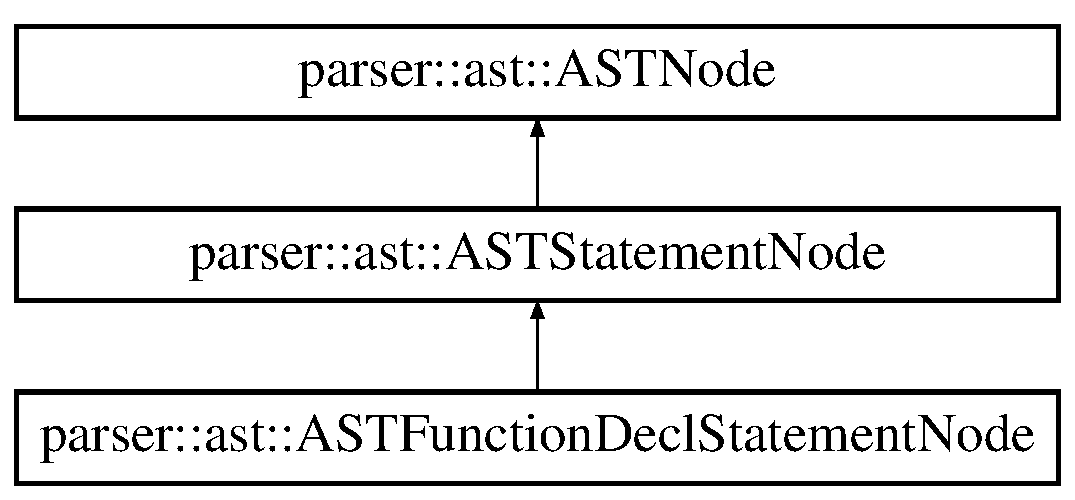
\includegraphics[height=3.000000cm]{d1/d41/classparser_1_1ast_1_1ASTFunctionDeclStatementNode}
\end{center}
\end{figure}
\subsection*{Public Member Functions}
\begin{DoxyCompactItemize}
\item 
\hyperlink{classparser_1_1ast_1_1ASTFunctionDeclStatementNode_ad03b8fb3eb6f05fa54f78aa362c1f89b}{A\+S\+T\+Function\+Decl\+Statement\+Node} (std\+::unique\+\_\+ptr$<$ \hyperlink{classparser_1_1ast_1_1ASTIdentifierNode}{A\+S\+T\+Identifier\+Node} $>$ \hyperlink{classparser_1_1ast_1_1ASTFunctionDeclStatementNode_a0a989fb6f81a61710fb6dcd0e8f8b627}{identifier}, std\+::vector$<$ std\+::pair$<$ std\+::unique\+\_\+ptr$<$ \hyperlink{classparser_1_1ast_1_1ASTIdentifierNode}{parser\+::ast\+::\+A\+S\+T\+Identifier\+Node} $>$, \hyperlink{ASTVariableDeclStatementNode_8h_a1e8e1bde0729627e3a22ffa858d5f3b9}{Variable\+Type} $>$$>$ \&params, \hyperlink{ASTVariableDeclStatementNode_8h_a1e8e1bde0729627e3a22ffa858d5f3b9}{Variable\+Type} \hyperlink{classparser_1_1ast_1_1ASTFunctionDeclStatementNode_a599bee08b41465e1787471f76069181f}{return\+Type}, std\+::unique\+\_\+ptr$<$ \hyperlink{classparser_1_1ast_1_1ASTBlockStatementNode}{A\+S\+T\+Block\+Statement\+Node} $>$ \hyperlink{classparser_1_1ast_1_1ASTFunctionDeclStatementNode_a9c6e0d925487c0f9b9770de8f84b0377}{block})
\item 
std\+::unique\+\_\+ptr$<$ \hyperlink{classparser_1_1ast_1_1ASTIdentifierNode}{A\+S\+T\+Identifier\+Node} $>$ \& \hyperlink{classparser_1_1ast_1_1ASTFunctionDeclStatementNode_a90b14f42d6e5c0e7ace537bc1ed079c1}{get\+Identifier} ()
\item 
std\+::vector$<$ std\+::pair$<$ std\+::unique\+\_\+ptr$<$ \hyperlink{classparser_1_1ast_1_1ASTIdentifierNode}{A\+S\+T\+Identifier\+Node} $>$, \hyperlink{ASTVariableDeclStatementNode_8h_a1e8e1bde0729627e3a22ffa858d5f3b9}{Variable\+Type} $>$ $>$ \& \hyperlink{classparser_1_1ast_1_1ASTFunctionDeclStatementNode_a21e415e1b48a5f95ce8efff983d35933}{get\+Formal\+Params} ()
\item 
\hyperlink{ASTVariableDeclStatementNode_8h_a1e8e1bde0729627e3a22ffa858d5f3b9}{Variable\+Type} \hyperlink{classparser_1_1ast_1_1ASTFunctionDeclStatementNode_a72b43b1559bc23654e186052d1f3edeb}{get\+Return\+Type} ()
\item 
std\+::unique\+\_\+ptr$<$ \hyperlink{classparser_1_1ast_1_1ASTBlockStatementNode}{A\+S\+T\+Block\+Statement\+Node} $>$ \& \hyperlink{classparser_1_1ast_1_1ASTFunctionDeclStatementNode_ac219fd306035b1f58373b29f80309f4b}{get\+Block} ()
\item 
Statement\+Type \hyperlink{classparser_1_1ast_1_1ASTFunctionDeclStatementNode_af951f3f6b2b47831a252bafe3dcb2a1f}{get\+Statement\+Type} () override
\item 
void \hyperlink{classparser_1_1ast_1_1ASTFunctionDeclStatementNode_ac7648205bc34d4cf7434274869d1b6a8}{accept} (\hyperlink{classvisitor_1_1Visitor}{visitor\+::\+Visitor} $\ast$visitor) override
\end{DoxyCompactItemize}
\subsection*{Protected Attributes}
\begin{DoxyCompactItemize}
\item 
\mbox{\Hypertarget{classparser_1_1ast_1_1ASTFunctionDeclStatementNode_a0a989fb6f81a61710fb6dcd0e8f8b627}\label{classparser_1_1ast_1_1ASTFunctionDeclStatementNode_a0a989fb6f81a61710fb6dcd0e8f8b627}} 
std\+::unique\+\_\+ptr$<$ \hyperlink{classparser_1_1ast_1_1ASTIdentifierNode}{A\+S\+T\+Identifier\+Node} $>$ \hyperlink{classparser_1_1ast_1_1ASTFunctionDeclStatementNode_a0a989fb6f81a61710fb6dcd0e8f8b627}{identifier}
\begin{DoxyCompactList}\small\item\em The function\textquotesingle{}s name. \end{DoxyCompactList}\item 
\mbox{\Hypertarget{classparser_1_1ast_1_1ASTFunctionDeclStatementNode_ab89bd3acd8be42103084a7043018a485}\label{classparser_1_1ast_1_1ASTFunctionDeclStatementNode_ab89bd3acd8be42103084a7043018a485}} 
std\+::vector$<$ std\+::pair$<$ std\+::unique\+\_\+ptr$<$ \hyperlink{classparser_1_1ast_1_1ASTIdentifierNode}{A\+S\+T\+Identifier\+Node} $>$, \hyperlink{ASTVariableDeclStatementNode_8h_a1e8e1bde0729627e3a22ffa858d5f3b9}{Variable\+Type} $>$ $>$ \hyperlink{classparser_1_1ast_1_1ASTFunctionDeclStatementNode_ab89bd3acd8be42103084a7043018a485}{formal\+Params}
\begin{DoxyCompactList}\small\item\em The function\textquotesingle{}s parameters. \end{DoxyCompactList}\item 
\mbox{\Hypertarget{classparser_1_1ast_1_1ASTFunctionDeclStatementNode_a599bee08b41465e1787471f76069181f}\label{classparser_1_1ast_1_1ASTFunctionDeclStatementNode_a599bee08b41465e1787471f76069181f}} 
\hyperlink{ASTVariableDeclStatementNode_8h_a1e8e1bde0729627e3a22ffa858d5f3b9}{Variable\+Type} \hyperlink{classparser_1_1ast_1_1ASTFunctionDeclStatementNode_a599bee08b41465e1787471f76069181f}{return\+Type}
\begin{DoxyCompactList}\small\item\em The return type. \end{DoxyCompactList}\item 
\mbox{\Hypertarget{classparser_1_1ast_1_1ASTFunctionDeclStatementNode_a9c6e0d925487c0f9b9770de8f84b0377}\label{classparser_1_1ast_1_1ASTFunctionDeclStatementNode_a9c6e0d925487c0f9b9770de8f84b0377}} 
std\+::unique\+\_\+ptr$<$ \hyperlink{classparser_1_1ast_1_1ASTBlockStatementNode}{A\+S\+T\+Block\+Statement\+Node} $>$ \hyperlink{classparser_1_1ast_1_1ASTFunctionDeclStatementNode_a9c6e0d925487c0f9b9770de8f84b0377}{block}
\begin{DoxyCompactList}\small\item\em The function block itself. \end{DoxyCompactList}\end{DoxyCompactItemize}


\subsection{Detailed Description}
This class represents a function declaration statement in the A\+ST 

\subsection{Constructor \& Destructor Documentation}
\mbox{\Hypertarget{classparser_1_1ast_1_1ASTFunctionDeclStatementNode_ad03b8fb3eb6f05fa54f78aa362c1f89b}\label{classparser_1_1ast_1_1ASTFunctionDeclStatementNode_ad03b8fb3eb6f05fa54f78aa362c1f89b}} 
\index{parser\+::ast\+::\+A\+S\+T\+Function\+Decl\+Statement\+Node@{parser\+::ast\+::\+A\+S\+T\+Function\+Decl\+Statement\+Node}!A\+S\+T\+Function\+Decl\+Statement\+Node@{A\+S\+T\+Function\+Decl\+Statement\+Node}}
\index{A\+S\+T\+Function\+Decl\+Statement\+Node@{A\+S\+T\+Function\+Decl\+Statement\+Node}!parser\+::ast\+::\+A\+S\+T\+Function\+Decl\+Statement\+Node@{parser\+::ast\+::\+A\+S\+T\+Function\+Decl\+Statement\+Node}}
\subsubsection{\texorpdfstring{A\+S\+T\+Function\+Decl\+Statement\+Node()}{ASTFunctionDeclStatementNode()}}
{\footnotesize\ttfamily parser\+::ast\+::\+A\+S\+T\+Function\+Decl\+Statement\+Node\+::\+A\+S\+T\+Function\+Decl\+Statement\+Node (\begin{DoxyParamCaption}\item[{std\+::unique\+\_\+ptr$<$ \hyperlink{classparser_1_1ast_1_1ASTIdentifierNode}{A\+S\+T\+Identifier\+Node} $>$}]{identifier,  }\item[{std\+::vector$<$ std\+::pair$<$ std\+::unique\+\_\+ptr$<$ \hyperlink{classparser_1_1ast_1_1ASTIdentifierNode}{parser\+::ast\+::\+A\+S\+T\+Identifier\+Node} $>$, \hyperlink{ASTVariableDeclStatementNode_8h_a1e8e1bde0729627e3a22ffa858d5f3b9}{Variable\+Type} $>$$>$ \&}]{params,  }\item[{\hyperlink{ASTVariableDeclStatementNode_8h_a1e8e1bde0729627e3a22ffa858d5f3b9}{Variable\+Type}}]{return\+Type,  }\item[{std\+::unique\+\_\+ptr$<$ \hyperlink{classparser_1_1ast_1_1ASTBlockStatementNode}{A\+S\+T\+Block\+Statement\+Node} $>$}]{block }\end{DoxyParamCaption})}

The constructor for this class 
\begin{DoxyParams}{Parameters}
{\em identifier} & The fucntion name \\
\hline
{\em params} & The formal parameters of the function \\
\hline
{\em return\+Type} & The return type of the function \\
\hline
{\em block} & The function block \\
\hline
\end{DoxyParams}


\subsection{Member Function Documentation}
\mbox{\Hypertarget{classparser_1_1ast_1_1ASTFunctionDeclStatementNode_ac7648205bc34d4cf7434274869d1b6a8}\label{classparser_1_1ast_1_1ASTFunctionDeclStatementNode_ac7648205bc34d4cf7434274869d1b6a8}} 
\index{parser\+::ast\+::\+A\+S\+T\+Function\+Decl\+Statement\+Node@{parser\+::ast\+::\+A\+S\+T\+Function\+Decl\+Statement\+Node}!accept@{accept}}
\index{accept@{accept}!parser\+::ast\+::\+A\+S\+T\+Function\+Decl\+Statement\+Node@{parser\+::ast\+::\+A\+S\+T\+Function\+Decl\+Statement\+Node}}
\subsubsection{\texorpdfstring{accept()}{accept()}}
{\footnotesize\ttfamily void parser\+::ast\+::\+A\+S\+T\+Function\+Decl\+Statement\+Node\+::accept (\begin{DoxyParamCaption}\item[{\hyperlink{classvisitor_1_1Visitor}{visitor\+::\+Visitor} $\ast$}]{visitor }\end{DoxyParamCaption})\hspace{0.3cm}{\ttfamily [override]}, {\ttfamily [virtual]}}

Accepts a visitor and calls the operation by invoking {\ttfamily visit(this)} 
\begin{DoxyParams}{Parameters}
{\em visitor} & the visitor to accept \\
\hline
\end{DoxyParams}


Implements \hyperlink{classparser_1_1ast_1_1ASTNode_a3ff84fdfdbbc5c39b70b4d04c22e7dc3}{parser\+::ast\+::\+A\+S\+T\+Node}.

\mbox{\Hypertarget{classparser_1_1ast_1_1ASTFunctionDeclStatementNode_ac219fd306035b1f58373b29f80309f4b}\label{classparser_1_1ast_1_1ASTFunctionDeclStatementNode_ac219fd306035b1f58373b29f80309f4b}} 
\index{parser\+::ast\+::\+A\+S\+T\+Function\+Decl\+Statement\+Node@{parser\+::ast\+::\+A\+S\+T\+Function\+Decl\+Statement\+Node}!get\+Block@{get\+Block}}
\index{get\+Block@{get\+Block}!parser\+::ast\+::\+A\+S\+T\+Function\+Decl\+Statement\+Node@{parser\+::ast\+::\+A\+S\+T\+Function\+Decl\+Statement\+Node}}
\subsubsection{\texorpdfstring{get\+Block()}{getBlock()}}
{\footnotesize\ttfamily std\+::unique\+\_\+ptr$<$ \hyperlink{classparser_1_1ast_1_1ASTBlockStatementNode}{parser\+::ast\+::\+A\+S\+T\+Block\+Statement\+Node} $>$ \& parser\+::ast\+::\+A\+S\+T\+Function\+Decl\+Statement\+Node\+::get\+Block (\begin{DoxyParamCaption}{ }\end{DoxyParamCaption})}

\begin{DoxyReturn}{Returns}
The function block 
\end{DoxyReturn}
\mbox{\Hypertarget{classparser_1_1ast_1_1ASTFunctionDeclStatementNode_a21e415e1b48a5f95ce8efff983d35933}\label{classparser_1_1ast_1_1ASTFunctionDeclStatementNode_a21e415e1b48a5f95ce8efff983d35933}} 
\index{parser\+::ast\+::\+A\+S\+T\+Function\+Decl\+Statement\+Node@{parser\+::ast\+::\+A\+S\+T\+Function\+Decl\+Statement\+Node}!get\+Formal\+Params@{get\+Formal\+Params}}
\index{get\+Formal\+Params@{get\+Formal\+Params}!parser\+::ast\+::\+A\+S\+T\+Function\+Decl\+Statement\+Node@{parser\+::ast\+::\+A\+S\+T\+Function\+Decl\+Statement\+Node}}
\subsubsection{\texorpdfstring{get\+Formal\+Params()}{getFormalParams()}}
{\footnotesize\ttfamily std\+::vector$<$ std\+::pair$<$ std\+::unique\+\_\+ptr$<$ \hyperlink{classparser_1_1ast_1_1ASTIdentifierNode}{parser\+::ast\+::\+A\+S\+T\+Identifier\+Node} $>$, \hyperlink{ASTVariableDeclStatementNode_8h_a1e8e1bde0729627e3a22ffa858d5f3b9}{parser\+::ast\+::\+Variable\+Type} $>$ $>$ \& parser\+::ast\+::\+A\+S\+T\+Function\+Decl\+Statement\+Node\+::get\+Formal\+Params (\begin{DoxyParamCaption}{ }\end{DoxyParamCaption})}

\begin{DoxyReturn}{Returns}
The function parameters 
\end{DoxyReturn}
\mbox{\Hypertarget{classparser_1_1ast_1_1ASTFunctionDeclStatementNode_a90b14f42d6e5c0e7ace537bc1ed079c1}\label{classparser_1_1ast_1_1ASTFunctionDeclStatementNode_a90b14f42d6e5c0e7ace537bc1ed079c1}} 
\index{parser\+::ast\+::\+A\+S\+T\+Function\+Decl\+Statement\+Node@{parser\+::ast\+::\+A\+S\+T\+Function\+Decl\+Statement\+Node}!get\+Identifier@{get\+Identifier}}
\index{get\+Identifier@{get\+Identifier}!parser\+::ast\+::\+A\+S\+T\+Function\+Decl\+Statement\+Node@{parser\+::ast\+::\+A\+S\+T\+Function\+Decl\+Statement\+Node}}
\subsubsection{\texorpdfstring{get\+Identifier()}{getIdentifier()}}
{\footnotesize\ttfamily std\+::unique\+\_\+ptr$<$ \hyperlink{classparser_1_1ast_1_1ASTIdentifierNode}{parser\+::ast\+::\+A\+S\+T\+Identifier\+Node} $>$ \& parser\+::ast\+::\+A\+S\+T\+Function\+Decl\+Statement\+Node\+::get\+Identifier (\begin{DoxyParamCaption}{ }\end{DoxyParamCaption})}

\begin{DoxyReturn}{Returns}
The function name 
\end{DoxyReturn}
\mbox{\Hypertarget{classparser_1_1ast_1_1ASTFunctionDeclStatementNode_a72b43b1559bc23654e186052d1f3edeb}\label{classparser_1_1ast_1_1ASTFunctionDeclStatementNode_a72b43b1559bc23654e186052d1f3edeb}} 
\index{parser\+::ast\+::\+A\+S\+T\+Function\+Decl\+Statement\+Node@{parser\+::ast\+::\+A\+S\+T\+Function\+Decl\+Statement\+Node}!get\+Return\+Type@{get\+Return\+Type}}
\index{get\+Return\+Type@{get\+Return\+Type}!parser\+::ast\+::\+A\+S\+T\+Function\+Decl\+Statement\+Node@{parser\+::ast\+::\+A\+S\+T\+Function\+Decl\+Statement\+Node}}
\subsubsection{\texorpdfstring{get\+Return\+Type()}{getReturnType()}}
{\footnotesize\ttfamily \hyperlink{ASTVariableDeclStatementNode_8h_a1e8e1bde0729627e3a22ffa858d5f3b9}{parser\+::ast\+::\+Variable\+Type} parser\+::ast\+::\+A\+S\+T\+Function\+Decl\+Statement\+Node\+::get\+Return\+Type (\begin{DoxyParamCaption}{ }\end{DoxyParamCaption})}

\begin{DoxyReturn}{Returns}
The function return type 
\end{DoxyReturn}
\mbox{\Hypertarget{classparser_1_1ast_1_1ASTFunctionDeclStatementNode_af951f3f6b2b47831a252bafe3dcb2a1f}\label{classparser_1_1ast_1_1ASTFunctionDeclStatementNode_af951f3f6b2b47831a252bafe3dcb2a1f}} 
\index{parser\+::ast\+::\+A\+S\+T\+Function\+Decl\+Statement\+Node@{parser\+::ast\+::\+A\+S\+T\+Function\+Decl\+Statement\+Node}!get\+Statement\+Type@{get\+Statement\+Type}}
\index{get\+Statement\+Type@{get\+Statement\+Type}!parser\+::ast\+::\+A\+S\+T\+Function\+Decl\+Statement\+Node@{parser\+::ast\+::\+A\+S\+T\+Function\+Decl\+Statement\+Node}}
\subsubsection{\texorpdfstring{get\+Statement\+Type()}{getStatementType()}}
{\footnotesize\ttfamily parser\+::ast\+::\+Statement\+Type parser\+::ast\+::\+A\+S\+T\+Function\+Decl\+Statement\+Node\+::get\+Statement\+Type (\begin{DoxyParamCaption}{ }\end{DoxyParamCaption})\hspace{0.3cm}{\ttfamily [override]}, {\ttfamily [virtual]}}

Virtual Method to return the statement type \begin{DoxyReturn}{Returns}
The statement type (instead of checking what class it\textquotesingle{}s an instance of) 
\end{DoxyReturn}


Implements \hyperlink{classparser_1_1ast_1_1ASTStatementNode_ac381d35d12f774a1bab0e209c5bfec1f}{parser\+::ast\+::\+A\+S\+T\+Statement\+Node}.



The documentation for this class was generated from the following files\+:\begin{DoxyCompactItemize}
\item 
parser/ast/statement/\hyperlink{ASTFunctionDeclStatementNode_8h}{A\+S\+T\+Function\+Decl\+Statement\+Node.\+h}\item 
parser/ast/statement/A\+S\+T\+Function\+Decl\+Statement\+Node.\+cpp\end{DoxyCompactItemize}

\hypertarget{classparser_1_1ast_1_1ASTIdentifierNode}{}\section{parser\+:\+:ast\+:\+:A\+S\+T\+Identifier\+Node Class Reference}
\label{classparser_1_1ast_1_1ASTIdentifierNode}\index{parser\+::ast\+::\+A\+S\+T\+Identifier\+Node@{parser\+::ast\+::\+A\+S\+T\+Identifier\+Node}}
Inheritance diagram for parser\+:\+:ast\+:\+:A\+S\+T\+Identifier\+Node\+:\begin{figure}[H]
\begin{center}
\leavevmode
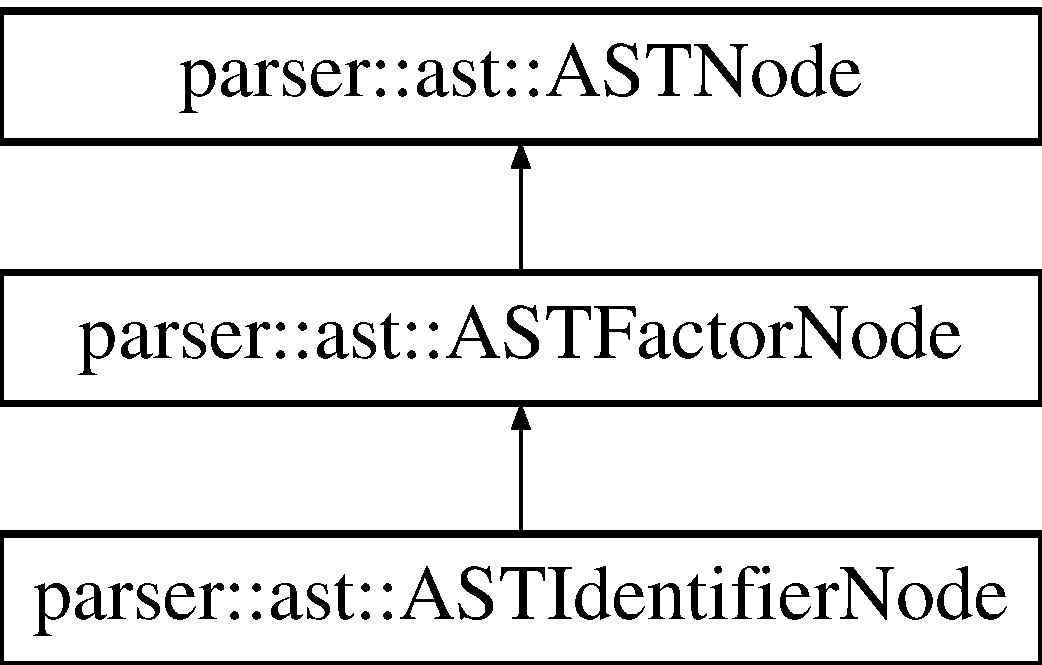
\includegraphics[height=3.000000cm]{da/d8b/classparser_1_1ast_1_1ASTIdentifierNode}
\end{center}
\end{figure}
\subsection*{Public Member Functions}
\begin{DoxyCompactItemize}
\item 
\hyperlink{classparser_1_1ast_1_1ASTIdentifierNode_a14e111874a3d1a5181f9d889e12106e5}{A\+S\+T\+Identifier\+Node} (const std\+::string \hyperlink{classparser_1_1ast_1_1ASTIdentifierNode_a3f8f65fc7806e99f8074fa7e0d1c0cf4}{name})
\item 
const std\+::string \hyperlink{classparser_1_1ast_1_1ASTIdentifierNode_adcb3da6c49adf6341e9a477458cc5998}{get\+Name} () const
\item 
\hyperlink{ASTFactorNode_8h_afbe2fcc03ef15b74a0c1ed1cda7ab0e8}{Factor\+Type} \hyperlink{classparser_1_1ast_1_1ASTIdentifierNode_a7b759817af29784741596a4387b6547f}{get\+Factor\+Type} () override
\item 
void \hyperlink{classparser_1_1ast_1_1ASTIdentifierNode_a45633268cd67b109e9b9cc6d565e48f3}{accept} (\hyperlink{classvisitor_1_1Visitor}{visitor\+::\+Visitor} $\ast$visitor) override
\end{DoxyCompactItemize}
\subsection*{Protected Attributes}
\begin{DoxyCompactItemize}
\item 
\mbox{\Hypertarget{classparser_1_1ast_1_1ASTIdentifierNode_a3f8f65fc7806e99f8074fa7e0d1c0cf4}\label{classparser_1_1ast_1_1ASTIdentifierNode_a3f8f65fc7806e99f8074fa7e0d1c0cf4}} 
std\+::string \hyperlink{classparser_1_1ast_1_1ASTIdentifierNode_a3f8f65fc7806e99f8074fa7e0d1c0cf4}{name}
\begin{DoxyCompactList}\small\item\em the identifier \end{DoxyCompactList}\end{DoxyCompactItemize}


\subsection{Constructor \& Destructor Documentation}
\mbox{\Hypertarget{classparser_1_1ast_1_1ASTIdentifierNode_a14e111874a3d1a5181f9d889e12106e5}\label{classparser_1_1ast_1_1ASTIdentifierNode_a14e111874a3d1a5181f9d889e12106e5}} 
\index{parser\+::ast\+::\+A\+S\+T\+Identifier\+Node@{parser\+::ast\+::\+A\+S\+T\+Identifier\+Node}!A\+S\+T\+Identifier\+Node@{A\+S\+T\+Identifier\+Node}}
\index{A\+S\+T\+Identifier\+Node@{A\+S\+T\+Identifier\+Node}!parser\+::ast\+::\+A\+S\+T\+Identifier\+Node@{parser\+::ast\+::\+A\+S\+T\+Identifier\+Node}}
\subsubsection{\texorpdfstring{A\+S\+T\+Identifier\+Node()}{ASTIdentifierNode()}}
{\footnotesize\ttfamily parser\+::ast\+::\+A\+S\+T\+Identifier\+Node\+::\+A\+S\+T\+Identifier\+Node (\begin{DoxyParamCaption}\item[{const std\+::string}]{name }\end{DoxyParamCaption})}

Construtor for this class 
\begin{DoxyParams}{Parameters}
{\em name} & the name of the identifier \\
\hline
\end{DoxyParams}


\subsection{Member Function Documentation}
\mbox{\Hypertarget{classparser_1_1ast_1_1ASTIdentifierNode_a45633268cd67b109e9b9cc6d565e48f3}\label{classparser_1_1ast_1_1ASTIdentifierNode_a45633268cd67b109e9b9cc6d565e48f3}} 
\index{parser\+::ast\+::\+A\+S\+T\+Identifier\+Node@{parser\+::ast\+::\+A\+S\+T\+Identifier\+Node}!accept@{accept}}
\index{accept@{accept}!parser\+::ast\+::\+A\+S\+T\+Identifier\+Node@{parser\+::ast\+::\+A\+S\+T\+Identifier\+Node}}
\subsubsection{\texorpdfstring{accept()}{accept()}}
{\footnotesize\ttfamily void parser\+::ast\+::\+A\+S\+T\+Identifier\+Node\+::accept (\begin{DoxyParamCaption}\item[{\hyperlink{classvisitor_1_1Visitor}{visitor\+::\+Visitor} $\ast$}]{visitor }\end{DoxyParamCaption})\hspace{0.3cm}{\ttfamily [override]}, {\ttfamily [virtual]}}

Accepts a visitor and calls the operation by invoking {\ttfamily visit(this)} 
\begin{DoxyParams}{Parameters}
{\em visitor} & the visitor to accept \\
\hline
\end{DoxyParams}


Implements \hyperlink{classparser_1_1ast_1_1ASTNode_a3ff84fdfdbbc5c39b70b4d04c22e7dc3}{parser\+::ast\+::\+A\+S\+T\+Node}.

\mbox{\Hypertarget{classparser_1_1ast_1_1ASTIdentifierNode_a7b759817af29784741596a4387b6547f}\label{classparser_1_1ast_1_1ASTIdentifierNode_a7b759817af29784741596a4387b6547f}} 
\index{parser\+::ast\+::\+A\+S\+T\+Identifier\+Node@{parser\+::ast\+::\+A\+S\+T\+Identifier\+Node}!get\+Factor\+Type@{get\+Factor\+Type}}
\index{get\+Factor\+Type@{get\+Factor\+Type}!parser\+::ast\+::\+A\+S\+T\+Identifier\+Node@{parser\+::ast\+::\+A\+S\+T\+Identifier\+Node}}
\subsubsection{\texorpdfstring{get\+Factor\+Type()}{getFactorType()}}
{\footnotesize\ttfamily \hyperlink{ASTFactorNode_8h_afbe2fcc03ef15b74a0c1ed1cda7ab0e8}{parser\+::ast\+::\+Factor\+Type} parser\+::ast\+::\+A\+S\+T\+Identifier\+Node\+::get\+Factor\+Type (\begin{DoxyParamCaption}{ }\end{DoxyParamCaption})\hspace{0.3cm}{\ttfamily [override]}, {\ttfamily [virtual]}}

\begin{DoxyReturn}{Returns}
The type of factor this is. Use instead of checking the class type. 
\end{DoxyReturn}


Implements \hyperlink{classparser_1_1ast_1_1ASTFactorNode_a13eea7f949c0055dea0a9d7b715f16a8}{parser\+::ast\+::\+A\+S\+T\+Factor\+Node}.

\mbox{\Hypertarget{classparser_1_1ast_1_1ASTIdentifierNode_adcb3da6c49adf6341e9a477458cc5998}\label{classparser_1_1ast_1_1ASTIdentifierNode_adcb3da6c49adf6341e9a477458cc5998}} 
\index{parser\+::ast\+::\+A\+S\+T\+Identifier\+Node@{parser\+::ast\+::\+A\+S\+T\+Identifier\+Node}!get\+Name@{get\+Name}}
\index{get\+Name@{get\+Name}!parser\+::ast\+::\+A\+S\+T\+Identifier\+Node@{parser\+::ast\+::\+A\+S\+T\+Identifier\+Node}}
\subsubsection{\texorpdfstring{get\+Name()}{getName()}}
{\footnotesize\ttfamily const std\+::string parser\+::ast\+::\+A\+S\+T\+Identifier\+Node\+::get\+Name (\begin{DoxyParamCaption}{ }\end{DoxyParamCaption}) const}

\begin{DoxyReturn}{Returns}
The name of the identifier 
\end{DoxyReturn}


The documentation for this class was generated from the following files\+:\begin{DoxyCompactItemize}
\item 
parser/ast/expression/factor/\hyperlink{ASTIdentifierNode_8h}{A\+S\+T\+Identifier\+Node.\+h}\item 
parser/ast/expression/factor/\hyperlink{ASTIdentifierNode_8cpp}{A\+S\+T\+Identifier\+Node.\+cpp}\end{DoxyCompactItemize}

\hypertarget{classparser_1_1ast_1_1ASTIfStatementNode}{}\section{parser\+:\+:ast\+:\+:A\+S\+T\+If\+Statement\+Node Class Reference}
\label{classparser_1_1ast_1_1ASTIfStatementNode}\index{parser\+::ast\+::\+A\+S\+T\+If\+Statement\+Node@{parser\+::ast\+::\+A\+S\+T\+If\+Statement\+Node}}


{\ttfamily \#include $<$A\+S\+T\+If\+Statement\+Node.\+h$>$}

Inheritance diagram for parser\+:\+:ast\+:\+:A\+S\+T\+If\+Statement\+Node\+:\begin{figure}[H]
\begin{center}
\leavevmode
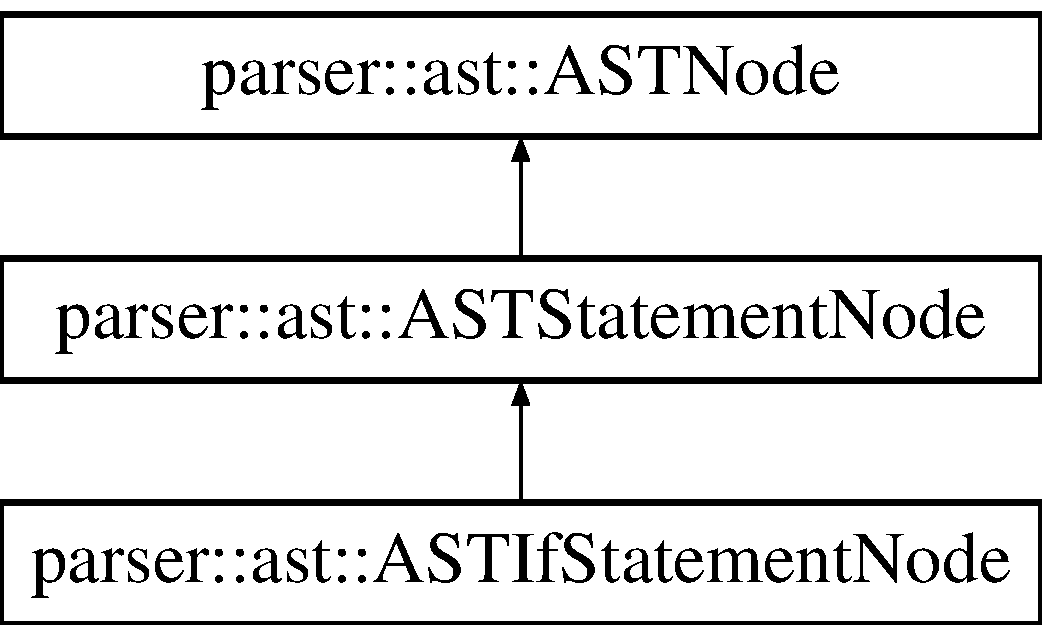
\includegraphics[height=3.000000cm]{d3/de4/classparser_1_1ast_1_1ASTIfStatementNode}
\end{center}
\end{figure}
\subsection*{Public Member Functions}
\begin{DoxyCompactItemize}
\item 
\hyperlink{classparser_1_1ast_1_1ASTIfStatementNode_a7a1228f06863f6c661941a718edf0f76}{A\+S\+T\+If\+Statement\+Node} (std\+::unique\+\_\+ptr$<$ \hyperlink{classparser_1_1ast_1_1ASTExprNode}{A\+S\+T\+Expr\+Node} $>$ \hyperlink{classparser_1_1ast_1_1ASTIfStatementNode_aa03b517ecf838b4ca92290f85873dacc}{predicate}, std\+::unique\+\_\+ptr$<$ \hyperlink{classparser_1_1ast_1_1ASTBlockStatementNode}{A\+S\+T\+Block\+Statement\+Node} $>$ \hyperlink{classparser_1_1ast_1_1ASTIfStatementNode_a41ce2a7eef7e04f060d06fd39b1634e9}{block\+If\+True}, std\+::unique\+\_\+ptr$<$ \hyperlink{classparser_1_1ast_1_1ASTBlockStatementNode}{A\+S\+T\+Block\+Statement\+Node} $>$ \hyperlink{classparser_1_1ast_1_1ASTIfStatementNode_a763d7c0df1b663ba69a38f5b744586f0}{block\+If\+False})
\item 
\hyperlink{classparser_1_1ast_1_1ASTIfStatementNode_a58f5fc968c7f49efa5acb3611af92696}{A\+S\+T\+If\+Statement\+Node} (std\+::unique\+\_\+ptr$<$ \hyperlink{classparser_1_1ast_1_1ASTExprNode}{A\+S\+T\+Expr\+Node} $>$ \hyperlink{classparser_1_1ast_1_1ASTIfStatementNode_aa03b517ecf838b4ca92290f85873dacc}{predicate}, std\+::unique\+\_\+ptr$<$ \hyperlink{classparser_1_1ast_1_1ASTBlockStatementNode}{A\+S\+T\+Block\+Statement\+Node} $>$ \hyperlink{classparser_1_1ast_1_1ASTIfStatementNode_a41ce2a7eef7e04f060d06fd39b1634e9}{block\+If\+True})
\item 
std\+::unique\+\_\+ptr$<$ \hyperlink{classparser_1_1ast_1_1ASTExprNode}{A\+S\+T\+Expr\+Node} $>$ \& \hyperlink{classparser_1_1ast_1_1ASTIfStatementNode_a709b472f90a91edf309c77cfc5fc0b25}{get\+Predicate} ()
\item 
std\+::unique\+\_\+ptr$<$ \hyperlink{classparser_1_1ast_1_1ASTBlockStatementNode}{A\+S\+T\+Block\+Statement\+Node} $>$ \& \hyperlink{classparser_1_1ast_1_1ASTIfStatementNode_a2db9e09e077f5fbb99c101ee0bf02887}{get\+Block\+If\+True} ()
\item 
std\+::unique\+\_\+ptr$<$ \hyperlink{classparser_1_1ast_1_1ASTBlockStatementNode}{A\+S\+T\+Block\+Statement\+Node} $>$ \& \hyperlink{classparser_1_1ast_1_1ASTIfStatementNode_a1f66f144fdb82bff3ead69fd563bcf73}{get\+Block\+If\+False} ()
\item 
Statement\+Type \hyperlink{classparser_1_1ast_1_1ASTIfStatementNode_aebe9139e5ee81c851aa01fd292635562}{get\+Statement\+Type} () override
\item 
void \hyperlink{classparser_1_1ast_1_1ASTIfStatementNode_a946a8196020e5d6c1a51a74d84d98e80}{accept} (\hyperlink{classvisitor_1_1Visitor}{visitor\+::\+Visitor} $\ast$visitor) override
\end{DoxyCompactItemize}
\subsection*{Protected Attributes}
\begin{DoxyCompactItemize}
\item 
\mbox{\Hypertarget{classparser_1_1ast_1_1ASTIfStatementNode_aa03b517ecf838b4ca92290f85873dacc}\label{classparser_1_1ast_1_1ASTIfStatementNode_aa03b517ecf838b4ca92290f85873dacc}} 
std\+::unique\+\_\+ptr$<$ \hyperlink{classparser_1_1ast_1_1ASTExprNode}{A\+S\+T\+Expr\+Node} $>$ \hyperlink{classparser_1_1ast_1_1ASTIfStatementNode_aa03b517ecf838b4ca92290f85873dacc}{predicate}
\begin{DoxyCompactList}\small\item\em The condition of the if statement. \end{DoxyCompactList}\item 
\mbox{\Hypertarget{classparser_1_1ast_1_1ASTIfStatementNode_a41ce2a7eef7e04f060d06fd39b1634e9}\label{classparser_1_1ast_1_1ASTIfStatementNode_a41ce2a7eef7e04f060d06fd39b1634e9}} 
std\+::unique\+\_\+ptr$<$ \hyperlink{classparser_1_1ast_1_1ASTBlockStatementNode}{A\+S\+T\+Block\+Statement\+Node} $>$ \hyperlink{classparser_1_1ast_1_1ASTIfStatementNode_a41ce2a7eef7e04f060d06fd39b1634e9}{block\+If\+True}
\begin{DoxyCompactList}\small\item\em The block to execute if the predicate holds. \end{DoxyCompactList}\item 
\mbox{\Hypertarget{classparser_1_1ast_1_1ASTIfStatementNode_a763d7c0df1b663ba69a38f5b744586f0}\label{classparser_1_1ast_1_1ASTIfStatementNode_a763d7c0df1b663ba69a38f5b744586f0}} 
std\+::unique\+\_\+ptr$<$ \hyperlink{classparser_1_1ast_1_1ASTBlockStatementNode}{A\+S\+T\+Block\+Statement\+Node} $>$ \hyperlink{classparser_1_1ast_1_1ASTIfStatementNode_a763d7c0df1b663ba69a38f5b744586f0}{block\+If\+False}
\begin{DoxyCompactList}\small\item\em The block to execute if the predicate does not hold. \end{DoxyCompactList}\end{DoxyCompactItemize}


\subsection{Detailed Description}
This class represents an \char`\"{}if else\char`\"{} statment in the A\+ST This would also represent an \char`\"{}if\char`\"{} statmement by not having an else block 

\subsection{Constructor \& Destructor Documentation}
\mbox{\Hypertarget{classparser_1_1ast_1_1ASTIfStatementNode_a7a1228f06863f6c661941a718edf0f76}\label{classparser_1_1ast_1_1ASTIfStatementNode_a7a1228f06863f6c661941a718edf0f76}} 
\index{parser\+::ast\+::\+A\+S\+T\+If\+Statement\+Node@{parser\+::ast\+::\+A\+S\+T\+If\+Statement\+Node}!A\+S\+T\+If\+Statement\+Node@{A\+S\+T\+If\+Statement\+Node}}
\index{A\+S\+T\+If\+Statement\+Node@{A\+S\+T\+If\+Statement\+Node}!parser\+::ast\+::\+A\+S\+T\+If\+Statement\+Node@{parser\+::ast\+::\+A\+S\+T\+If\+Statement\+Node}}
\subsubsection{\texorpdfstring{A\+S\+T\+If\+Statement\+Node()}{ASTIfStatementNode()}\hspace{0.1cm}{\footnotesize\ttfamily [1/2]}}
{\footnotesize\ttfamily parser\+::ast\+::\+A\+S\+T\+If\+Statement\+Node\+::\+A\+S\+T\+If\+Statement\+Node (\begin{DoxyParamCaption}\item[{std\+::unique\+\_\+ptr$<$ \hyperlink{classparser_1_1ast_1_1ASTExprNode}{A\+S\+T\+Expr\+Node} $>$}]{predicate,  }\item[{std\+::unique\+\_\+ptr$<$ \hyperlink{classparser_1_1ast_1_1ASTBlockStatementNode}{A\+S\+T\+Block\+Statement\+Node} $>$}]{block\+If\+True,  }\item[{std\+::unique\+\_\+ptr$<$ \hyperlink{classparser_1_1ast_1_1ASTBlockStatementNode}{A\+S\+T\+Block\+Statement\+Node} $>$}]{block\+If\+False }\end{DoxyParamCaption})}

This is the constructor for an if-\/else statmeent 
\begin{DoxyParams}{Parameters}
{\em predicate} & The condition to the if statement \\
\hline
{\em block\+If\+True} & The block to execute if the predicate holds \\
\hline
{\em block\+If\+False} & The block to exiecute if the predicate does not hold \\
\hline
\end{DoxyParams}
\mbox{\Hypertarget{classparser_1_1ast_1_1ASTIfStatementNode_a58f5fc968c7f49efa5acb3611af92696}\label{classparser_1_1ast_1_1ASTIfStatementNode_a58f5fc968c7f49efa5acb3611af92696}} 
\index{parser\+::ast\+::\+A\+S\+T\+If\+Statement\+Node@{parser\+::ast\+::\+A\+S\+T\+If\+Statement\+Node}!A\+S\+T\+If\+Statement\+Node@{A\+S\+T\+If\+Statement\+Node}}
\index{A\+S\+T\+If\+Statement\+Node@{A\+S\+T\+If\+Statement\+Node}!parser\+::ast\+::\+A\+S\+T\+If\+Statement\+Node@{parser\+::ast\+::\+A\+S\+T\+If\+Statement\+Node}}
\subsubsection{\texorpdfstring{A\+S\+T\+If\+Statement\+Node()}{ASTIfStatementNode()}\hspace{0.1cm}{\footnotesize\ttfamily [2/2]}}
{\footnotesize\ttfamily parser\+::ast\+::\+A\+S\+T\+If\+Statement\+Node\+::\+A\+S\+T\+If\+Statement\+Node (\begin{DoxyParamCaption}\item[{std\+::unique\+\_\+ptr$<$ \hyperlink{classparser_1_1ast_1_1ASTExprNode}{A\+S\+T\+Expr\+Node} $>$}]{predicate,  }\item[{std\+::unique\+\_\+ptr$<$ \hyperlink{classparser_1_1ast_1_1ASTBlockStatementNode}{A\+S\+T\+Block\+Statement\+Node} $>$}]{block\+If\+True }\end{DoxyParamCaption})}

This is the constructor for an if statmeent 
\begin{DoxyParams}{Parameters}
{\em predicate} & The condition to the if statement \\
\hline
{\em block\+If\+True} & The block to execute if the predicate holds \\
\hline
\end{DoxyParams}


\subsection{Member Function Documentation}
\mbox{\Hypertarget{classparser_1_1ast_1_1ASTIfStatementNode_a946a8196020e5d6c1a51a74d84d98e80}\label{classparser_1_1ast_1_1ASTIfStatementNode_a946a8196020e5d6c1a51a74d84d98e80}} 
\index{parser\+::ast\+::\+A\+S\+T\+If\+Statement\+Node@{parser\+::ast\+::\+A\+S\+T\+If\+Statement\+Node}!accept@{accept}}
\index{accept@{accept}!parser\+::ast\+::\+A\+S\+T\+If\+Statement\+Node@{parser\+::ast\+::\+A\+S\+T\+If\+Statement\+Node}}
\subsubsection{\texorpdfstring{accept()}{accept()}}
{\footnotesize\ttfamily void parser\+::ast\+::\+A\+S\+T\+If\+Statement\+Node\+::accept (\begin{DoxyParamCaption}\item[{\hyperlink{classvisitor_1_1Visitor}{visitor\+::\+Visitor} $\ast$}]{visitor }\end{DoxyParamCaption})\hspace{0.3cm}{\ttfamily [override]}, {\ttfamily [virtual]}}

Accepts a visitor and calls the operation by invoking {\ttfamily visit(this)} 
\begin{DoxyParams}{Parameters}
{\em visitor} & the visitor to accept \\
\hline
\end{DoxyParams}


Implements \hyperlink{classparser_1_1ast_1_1ASTNode_a3ff84fdfdbbc5c39b70b4d04c22e7dc3}{parser\+::ast\+::\+A\+S\+T\+Node}.

\mbox{\Hypertarget{classparser_1_1ast_1_1ASTIfStatementNode_a1f66f144fdb82bff3ead69fd563bcf73}\label{classparser_1_1ast_1_1ASTIfStatementNode_a1f66f144fdb82bff3ead69fd563bcf73}} 
\index{parser\+::ast\+::\+A\+S\+T\+If\+Statement\+Node@{parser\+::ast\+::\+A\+S\+T\+If\+Statement\+Node}!get\+Block\+If\+False@{get\+Block\+If\+False}}
\index{get\+Block\+If\+False@{get\+Block\+If\+False}!parser\+::ast\+::\+A\+S\+T\+If\+Statement\+Node@{parser\+::ast\+::\+A\+S\+T\+If\+Statement\+Node}}
\subsubsection{\texorpdfstring{get\+Block\+If\+False()}{getBlockIfFalse()}}
{\footnotesize\ttfamily std\+::unique\+\_\+ptr$<$ \hyperlink{classparser_1_1ast_1_1ASTBlockStatementNode}{parser\+::ast\+::\+A\+S\+T\+Block\+Statement\+Node} $>$ \& parser\+::ast\+::\+A\+S\+T\+If\+Statement\+Node\+::get\+Block\+If\+False (\begin{DoxyParamCaption}{ }\end{DoxyParamCaption})}

\begin{DoxyReturn}{Returns}
The block to execute if the predicate does not hold 
\end{DoxyReturn}
\mbox{\Hypertarget{classparser_1_1ast_1_1ASTIfStatementNode_a2db9e09e077f5fbb99c101ee0bf02887}\label{classparser_1_1ast_1_1ASTIfStatementNode_a2db9e09e077f5fbb99c101ee0bf02887}} 
\index{parser\+::ast\+::\+A\+S\+T\+If\+Statement\+Node@{parser\+::ast\+::\+A\+S\+T\+If\+Statement\+Node}!get\+Block\+If\+True@{get\+Block\+If\+True}}
\index{get\+Block\+If\+True@{get\+Block\+If\+True}!parser\+::ast\+::\+A\+S\+T\+If\+Statement\+Node@{parser\+::ast\+::\+A\+S\+T\+If\+Statement\+Node}}
\subsubsection{\texorpdfstring{get\+Block\+If\+True()}{getBlockIfTrue()}}
{\footnotesize\ttfamily std\+::unique\+\_\+ptr$<$ \hyperlink{classparser_1_1ast_1_1ASTBlockStatementNode}{parser\+::ast\+::\+A\+S\+T\+Block\+Statement\+Node} $>$ \& parser\+::ast\+::\+A\+S\+T\+If\+Statement\+Node\+::get\+Block\+If\+True (\begin{DoxyParamCaption}{ }\end{DoxyParamCaption})}

\begin{DoxyReturn}{Returns}
The block to execute if the predicate holds 
\end{DoxyReturn}
\mbox{\Hypertarget{classparser_1_1ast_1_1ASTIfStatementNode_a709b472f90a91edf309c77cfc5fc0b25}\label{classparser_1_1ast_1_1ASTIfStatementNode_a709b472f90a91edf309c77cfc5fc0b25}} 
\index{parser\+::ast\+::\+A\+S\+T\+If\+Statement\+Node@{parser\+::ast\+::\+A\+S\+T\+If\+Statement\+Node}!get\+Predicate@{get\+Predicate}}
\index{get\+Predicate@{get\+Predicate}!parser\+::ast\+::\+A\+S\+T\+If\+Statement\+Node@{parser\+::ast\+::\+A\+S\+T\+If\+Statement\+Node}}
\subsubsection{\texorpdfstring{get\+Predicate()}{getPredicate()}}
{\footnotesize\ttfamily std\+::unique\+\_\+ptr$<$ \hyperlink{classparser_1_1ast_1_1ASTExprNode}{parser\+::ast\+::\+A\+S\+T\+Expr\+Node} $>$ \& parser\+::ast\+::\+A\+S\+T\+If\+Statement\+Node\+::get\+Predicate (\begin{DoxyParamCaption}{ }\end{DoxyParamCaption})}

\begin{DoxyReturn}{Returns}
The predicate expression of the if statement 
\end{DoxyReturn}
\mbox{\Hypertarget{classparser_1_1ast_1_1ASTIfStatementNode_aebe9139e5ee81c851aa01fd292635562}\label{classparser_1_1ast_1_1ASTIfStatementNode_aebe9139e5ee81c851aa01fd292635562}} 
\index{parser\+::ast\+::\+A\+S\+T\+If\+Statement\+Node@{parser\+::ast\+::\+A\+S\+T\+If\+Statement\+Node}!get\+Statement\+Type@{get\+Statement\+Type}}
\index{get\+Statement\+Type@{get\+Statement\+Type}!parser\+::ast\+::\+A\+S\+T\+If\+Statement\+Node@{parser\+::ast\+::\+A\+S\+T\+If\+Statement\+Node}}
\subsubsection{\texorpdfstring{get\+Statement\+Type()}{getStatementType()}}
{\footnotesize\ttfamily parser\+::ast\+::\+Statement\+Type parser\+::ast\+::\+A\+S\+T\+If\+Statement\+Node\+::get\+Statement\+Type (\begin{DoxyParamCaption}{ }\end{DoxyParamCaption})\hspace{0.3cm}{\ttfamily [override]}, {\ttfamily [virtual]}}

Virtual Method to return the statement type \begin{DoxyReturn}{Returns}
The statement type (instead of checking what class it\textquotesingle{}s an instance of) 
\end{DoxyReturn}


Implements \hyperlink{classparser_1_1ast_1_1ASTStatementNode_ac381d35d12f774a1bab0e209c5bfec1f}{parser\+::ast\+::\+A\+S\+T\+Statement\+Node}.



The documentation for this class was generated from the following files\+:\begin{DoxyCompactItemize}
\item 
parser/ast/statement/\hyperlink{ASTIfStatementNode_8h}{A\+S\+T\+If\+Statement\+Node.\+h}\item 
parser/ast/statement/A\+S\+T\+If\+Statement\+Node.\+cpp\end{DoxyCompactItemize}

\hypertarget{classparser_1_1ast_1_1ASTLiteralNode}{}\section{parser\+:\+:ast\+:\+:A\+S\+T\+Literal\+Node$<$ T $>$ Class Template Reference}
\label{classparser_1_1ast_1_1ASTLiteralNode}\index{parser\+::ast\+::\+A\+S\+T\+Literal\+Node$<$ T $>$@{parser\+::ast\+::\+A\+S\+T\+Literal\+Node$<$ T $>$}}


{\ttfamily \#include $<$A\+S\+T\+Literal\+Node.\+h$>$}

Inheritance diagram for parser\+:\+:ast\+:\+:A\+S\+T\+Literal\+Node$<$ T $>$\+:\begin{figure}[H]
\begin{center}
\leavevmode
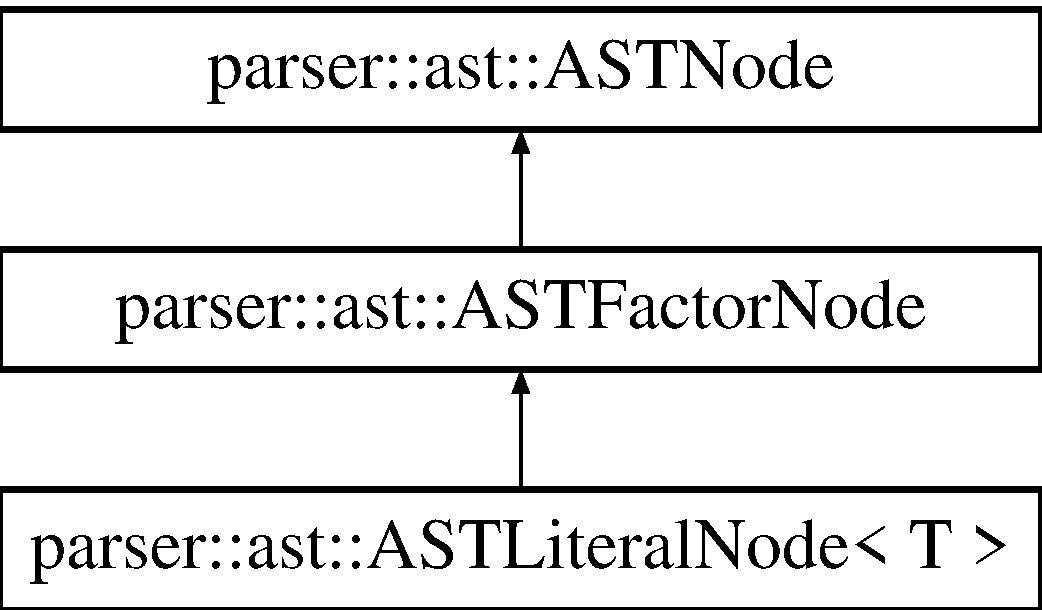
\includegraphics[height=3.000000cm]{dc/d86/classparser_1_1ast_1_1ASTLiteralNode}
\end{center}
\end{figure}
\subsection*{Public Member Functions}
\begin{DoxyCompactItemize}
\item 
\hyperlink{classparser_1_1ast_1_1ASTLiteralNode_a44d0a5e92c58efc35fb9778b56feb725}{A\+S\+T\+Literal\+Node} (T literal)
\item 
T \hyperlink{classparser_1_1ast_1_1ASTLiteralNode_a43466bd413257d43650659383351e612}{get\+Literal} () const
\item 
\hyperlink{ASTFactorNode_8h_afbe2fcc03ef15b74a0c1ed1cda7ab0e8}{Factor\+Type} \hyperlink{classparser_1_1ast_1_1ASTLiteralNode_a08efdbff5f7b0a0b7623ad964a6e4a9f}{get\+Factor\+Type} () override
\item 
void \hyperlink{classparser_1_1ast_1_1ASTLiteralNode_a6d7a907614e19132b9c669f7aa32b735}{accept} (\hyperlink{classvisitor_1_1Visitor}{visitor\+::\+Visitor} $\ast$visitor) override
\end{DoxyCompactItemize}
\subsection*{Protected Attributes}
\begin{DoxyCompactItemize}
\item 
\mbox{\Hypertarget{classparser_1_1ast_1_1ASTLiteralNode_a3d8332043910f9f6d068c5c22814a13f}\label{classparser_1_1ast_1_1ASTLiteralNode_a3d8332043910f9f6d068c5c22814a13f}} 
T {\bfseries literal}
\end{DoxyCompactItemize}


\subsection{Detailed Description}
\subsubsection*{template$<$typename T$>$\newline
class parser\+::ast\+::\+A\+S\+T\+Literal\+Node$<$ T $>$}

Class representing a literal node in the A\+ST 

\subsection{Constructor \& Destructor Documentation}
\mbox{\Hypertarget{classparser_1_1ast_1_1ASTLiteralNode_a44d0a5e92c58efc35fb9778b56feb725}\label{classparser_1_1ast_1_1ASTLiteralNode_a44d0a5e92c58efc35fb9778b56feb725}} 
\index{parser\+::ast\+::\+A\+S\+T\+Literal\+Node@{parser\+::ast\+::\+A\+S\+T\+Literal\+Node}!A\+S\+T\+Literal\+Node@{A\+S\+T\+Literal\+Node}}
\index{A\+S\+T\+Literal\+Node@{A\+S\+T\+Literal\+Node}!parser\+::ast\+::\+A\+S\+T\+Literal\+Node@{parser\+::ast\+::\+A\+S\+T\+Literal\+Node}}
\subsubsection{\texorpdfstring{A\+S\+T\+Literal\+Node()}{ASTLiteralNode()}}
{\footnotesize\ttfamily template$<$typename T $>$ \\
\hyperlink{classparser_1_1ast_1_1ASTLiteralNode}{parser\+::ast\+::\+A\+S\+T\+Literal\+Node}$<$ T $>$\+::\hyperlink{classparser_1_1ast_1_1ASTLiteralNode}{A\+S\+T\+Literal\+Node} (\begin{DoxyParamCaption}\item[{T}]{literal }\end{DoxyParamCaption})}

Constructor for this literal 
\begin{DoxyParams}{Parameters}
{\em literal} & The literal to store \\
\hline
\end{DoxyParams}


\subsection{Member Function Documentation}
\mbox{\Hypertarget{classparser_1_1ast_1_1ASTLiteralNode_a6d7a907614e19132b9c669f7aa32b735}\label{classparser_1_1ast_1_1ASTLiteralNode_a6d7a907614e19132b9c669f7aa32b735}} 
\index{parser\+::ast\+::\+A\+S\+T\+Literal\+Node@{parser\+::ast\+::\+A\+S\+T\+Literal\+Node}!accept@{accept}}
\index{accept@{accept}!parser\+::ast\+::\+A\+S\+T\+Literal\+Node@{parser\+::ast\+::\+A\+S\+T\+Literal\+Node}}
\subsubsection{\texorpdfstring{accept()}{accept()}}
{\footnotesize\ttfamily template$<$typename T $>$ \\
void \hyperlink{classparser_1_1ast_1_1ASTLiteralNode}{parser\+::ast\+::\+A\+S\+T\+Literal\+Node}$<$ T $>$\+::accept (\begin{DoxyParamCaption}\item[{\hyperlink{classvisitor_1_1Visitor}{visitor\+::\+Visitor} $\ast$}]{visitor }\end{DoxyParamCaption})\hspace{0.3cm}{\ttfamily [override]}, {\ttfamily [virtual]}}

Accepts a visitor and calls the operation by invoking {\ttfamily visit(this)} 
\begin{DoxyParams}{Parameters}
{\em visitor} & the visitor to accept \\
\hline
\end{DoxyParams}


Implements \hyperlink{classparser_1_1ast_1_1ASTNode_a3ff84fdfdbbc5c39b70b4d04c22e7dc3}{parser\+::ast\+::\+A\+S\+T\+Node}.

\mbox{\Hypertarget{classparser_1_1ast_1_1ASTLiteralNode_a08efdbff5f7b0a0b7623ad964a6e4a9f}\label{classparser_1_1ast_1_1ASTLiteralNode_a08efdbff5f7b0a0b7623ad964a6e4a9f}} 
\index{parser\+::ast\+::\+A\+S\+T\+Literal\+Node@{parser\+::ast\+::\+A\+S\+T\+Literal\+Node}!get\+Factor\+Type@{get\+Factor\+Type}}
\index{get\+Factor\+Type@{get\+Factor\+Type}!parser\+::ast\+::\+A\+S\+T\+Literal\+Node@{parser\+::ast\+::\+A\+S\+T\+Literal\+Node}}
\subsubsection{\texorpdfstring{get\+Factor\+Type()}{getFactorType()}}
{\footnotesize\ttfamily template$<$typename T $>$ \\
\hyperlink{ASTFactorNode_8h_afbe2fcc03ef15b74a0c1ed1cda7ab0e8}{parser\+::ast\+::\+Factor\+Type} \hyperlink{classparser_1_1ast_1_1ASTLiteralNode}{parser\+::ast\+::\+A\+S\+T\+Literal\+Node}$<$ T $>$\+::get\+Factor\+Type (\begin{DoxyParamCaption}{ }\end{DoxyParamCaption})\hspace{0.3cm}{\ttfamily [override]}, {\ttfamily [virtual]}}

\begin{DoxyReturn}{Returns}
The type of factor this is. Use instead of checking the class type. 
\end{DoxyReturn}


Implements \hyperlink{classparser_1_1ast_1_1ASTFactorNode_a13eea7f949c0055dea0a9d7b715f16a8}{parser\+::ast\+::\+A\+S\+T\+Factor\+Node}.

\mbox{\Hypertarget{classparser_1_1ast_1_1ASTLiteralNode_a43466bd413257d43650659383351e612}\label{classparser_1_1ast_1_1ASTLiteralNode_a43466bd413257d43650659383351e612}} 
\index{parser\+::ast\+::\+A\+S\+T\+Literal\+Node@{parser\+::ast\+::\+A\+S\+T\+Literal\+Node}!get\+Literal@{get\+Literal}}
\index{get\+Literal@{get\+Literal}!parser\+::ast\+::\+A\+S\+T\+Literal\+Node@{parser\+::ast\+::\+A\+S\+T\+Literal\+Node}}
\subsubsection{\texorpdfstring{get\+Literal()}{getLiteral()}}
{\footnotesize\ttfamily template$<$typename T $>$ \\
T \hyperlink{classparser_1_1ast_1_1ASTLiteralNode}{parser\+::ast\+::\+A\+S\+T\+Literal\+Node}$<$ T $>$\+::get\+Literal (\begin{DoxyParamCaption}{ }\end{DoxyParamCaption}) const}

\begin{DoxyReturn}{Returns}
the literal 
\end{DoxyReturn}


The documentation for this class was generated from the following files\+:\begin{DoxyCompactItemize}
\item 
parser/ast/expression/factor/\hyperlink{ASTLiteralNode_8h}{A\+S\+T\+Literal\+Node.\+h}\item 
parser/ast/expression/factor/\hyperlink{ASTLiteralNode_8cpp}{A\+S\+T\+Literal\+Node.\+cpp}\end{DoxyCompactItemize}

\hypertarget{classparser_1_1ast_1_1ASTNode}{}\section{parser\+:\+:ast\+:\+:A\+S\+T\+Node Class Reference}
\label{classparser_1_1ast_1_1ASTNode}\index{parser\+::ast\+::\+A\+S\+T\+Node@{parser\+::ast\+::\+A\+S\+T\+Node}}
Inheritance diagram for parser\+:\+:ast\+:\+:A\+S\+T\+Node\+:\begin{figure}[H]
\begin{center}
\leavevmode
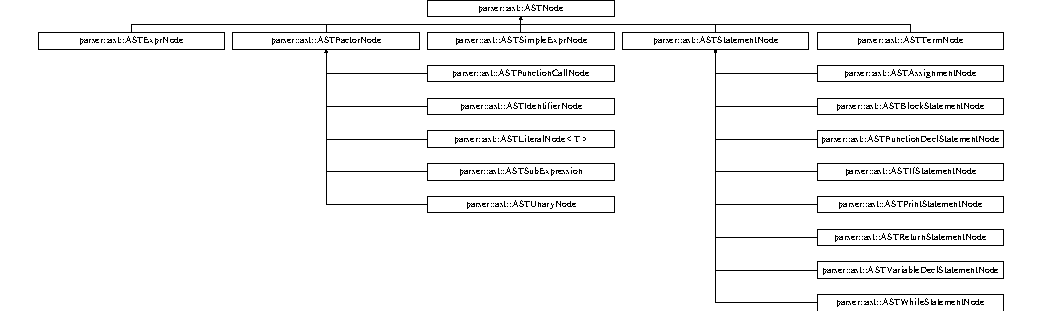
\includegraphics[height=4.179105cm]{da/d7c/classparser_1_1ast_1_1ASTNode}
\end{center}
\end{figure}
\subsection*{Public Member Functions}
\begin{DoxyCompactItemize}
\item 
virtual void \hyperlink{classparser_1_1ast_1_1ASTNode_a3ff84fdfdbbc5c39b70b4d04c22e7dc3}{accept} (\hyperlink{classvisitor_1_1Visitor}{visitor\+::\+Visitor} $\ast$visitor)=0
\end{DoxyCompactItemize}


\subsection{Member Function Documentation}
\mbox{\Hypertarget{classparser_1_1ast_1_1ASTNode_a3ff84fdfdbbc5c39b70b4d04c22e7dc3}\label{classparser_1_1ast_1_1ASTNode_a3ff84fdfdbbc5c39b70b4d04c22e7dc3}} 
\index{parser\+::ast\+::\+A\+S\+T\+Node@{parser\+::ast\+::\+A\+S\+T\+Node}!accept@{accept}}
\index{accept@{accept}!parser\+::ast\+::\+A\+S\+T\+Node@{parser\+::ast\+::\+A\+S\+T\+Node}}
\subsubsection{\texorpdfstring{accept()}{accept()}}
{\footnotesize\ttfamily virtual void parser\+::ast\+::\+A\+S\+T\+Node\+::accept (\begin{DoxyParamCaption}\item[{\hyperlink{classvisitor_1_1Visitor}{visitor\+::\+Visitor} $\ast$}]{visitor }\end{DoxyParamCaption})\hspace{0.3cm}{\ttfamily [pure virtual]}}

Accepts a visitor and calls the operation by invoking {\ttfamily visit(this)} 
\begin{DoxyParams}{Parameters}
{\em visitor} & the visitor to accept \\
\hline
\end{DoxyParams}


Implemented in \hyperlink{classparser_1_1ast_1_1ASTVariableDeclStatementNode_a4448c73408ed86719c6f3993a4eb8869}{parser\+::ast\+::\+A\+S\+T\+Variable\+Decl\+Statement\+Node}, \hyperlink{classparser_1_1ast_1_1ASTSimpleExprNode_a493a0e358cc89eb16f7a7ae9982d6527}{parser\+::ast\+::\+A\+S\+T\+Simple\+Expr\+Node}, \hyperlink{classparser_1_1ast_1_1ASTExprNode_a3eea258af04a74930acc0c9fb6aade77}{parser\+::ast\+::\+A\+S\+T\+Expr\+Node}, \hyperlink{classparser_1_1ast_1_1ASTTermNode_a4937651cff0fac499c76f8f38fa4795d}{parser\+::ast\+::\+A\+S\+T\+Term\+Node}, \hyperlink{classparser_1_1ast_1_1ASTFunctionDeclStatementNode_ac7648205bc34d4cf7434274869d1b6a8}{parser\+::ast\+::\+A\+S\+T\+Function\+Decl\+Statement\+Node}, \hyperlink{classparser_1_1ast_1_1ASTIfStatementNode_a946a8196020e5d6c1a51a74d84d98e80}{parser\+::ast\+::\+A\+S\+T\+If\+Statement\+Node}, \hyperlink{classparser_1_1ast_1_1ASTUnaryNode_a4b3bd9c26548e1fb73a82fd5b20add0b}{parser\+::ast\+::\+A\+S\+T\+Unary\+Node}, \hyperlink{classparser_1_1ast_1_1ASTAssignmentNode_abfbf5dd90191738f1faea1334fe8480b}{parser\+::ast\+::\+A\+S\+T\+Assignment\+Node}, \hyperlink{classparser_1_1ast_1_1ASTWhileStatementNode_a448a46d9dbde688562ada266192735c8}{parser\+::ast\+::\+A\+S\+T\+While\+Statement\+Node}, \hyperlink{classparser_1_1ast_1_1ASTFunctionCallNode_ad7ff48d8398744b1211a6da0399a197b}{parser\+::ast\+::\+A\+S\+T\+Function\+Call\+Node}, \hyperlink{classparser_1_1ast_1_1ASTLiteralNode_a6d7a907614e19132b9c669f7aa32b735}{parser\+::ast\+::\+A\+S\+T\+Literal\+Node$<$ T $>$}, \hyperlink{classparser_1_1ast_1_1ASTSubExpression_a684e39e8385690e9bade65731ba5803b}{parser\+::ast\+::\+A\+S\+T\+Sub\+Expression}, \hyperlink{classparser_1_1ast_1_1ASTReturnStatementNode_ac66c375bc67277468711fdec08e93b15}{parser\+::ast\+::\+A\+S\+T\+Return\+Statement\+Node}, \hyperlink{classparser_1_1ast_1_1ASTIdentifierNode_a45633268cd67b109e9b9cc6d565e48f3}{parser\+::ast\+::\+A\+S\+T\+Identifier\+Node}, \hyperlink{classparser_1_1ast_1_1ASTBlockStatementNode_ae0e7e04747661471aade0c1509c37422}{parser\+::ast\+::\+A\+S\+T\+Block\+Statement\+Node}, and \hyperlink{classparser_1_1ast_1_1ASTPrintStatementNode_a15199624d689c55bd6d027132d2a9a64}{parser\+::ast\+::\+A\+S\+T\+Print\+Statement\+Node}.



The documentation for this class was generated from the following file\+:\begin{DoxyCompactItemize}
\item 
parser/ast/A\+S\+T\+Node.\+h\end{DoxyCompactItemize}

\hypertarget{classparser_1_1ast_1_1ASTPrintStatementNode}{}\section{parser\+:\+:ast\+:\+:A\+S\+T\+Print\+Statement\+Node Class Reference}
\label{classparser_1_1ast_1_1ASTPrintStatementNode}\index{parser\+::ast\+::\+A\+S\+T\+Print\+Statement\+Node@{parser\+::ast\+::\+A\+S\+T\+Print\+Statement\+Node}}


{\ttfamily \#include $<$A\+S\+T\+Print\+Statement\+Node.\+h$>$}

Inheritance diagram for parser\+:\+:ast\+:\+:A\+S\+T\+Print\+Statement\+Node\+:\begin{figure}[H]
\begin{center}
\leavevmode
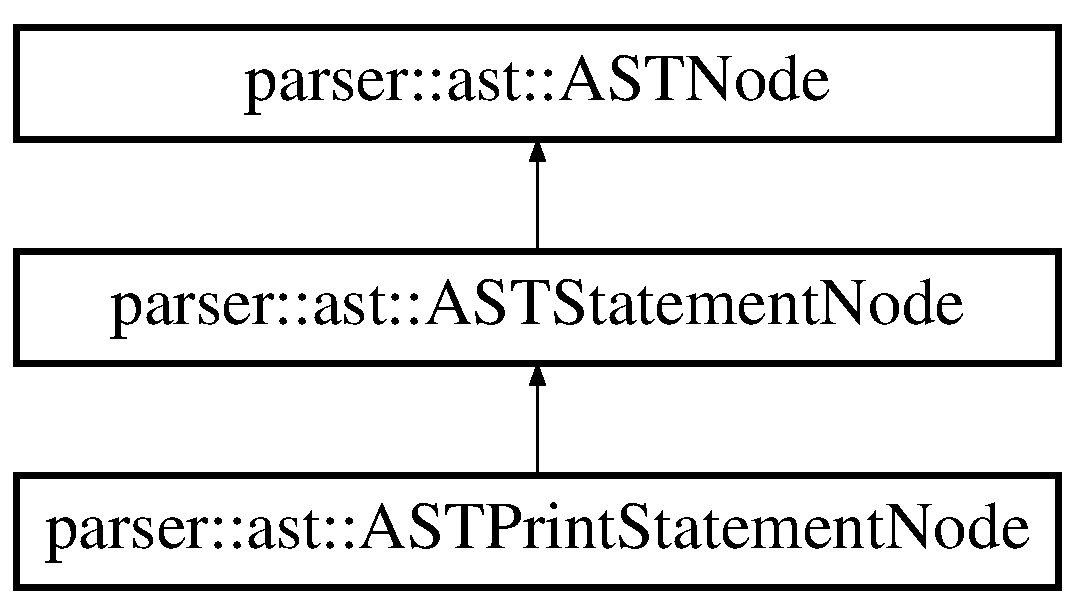
\includegraphics[height=3.000000cm]{d0/d40/classparser_1_1ast_1_1ASTPrintStatementNode}
\end{center}
\end{figure}
\subsection*{Public Member Functions}
\begin{DoxyCompactItemize}
\item 
\hyperlink{classparser_1_1ast_1_1ASTPrintStatementNode_a078c63cee6196eb39232a1004614f2f2}{A\+S\+T\+Print\+Statement\+Node} (std\+::unique\+\_\+ptr$<$ \hyperlink{classparser_1_1ast_1_1ASTExprNode}{A\+S\+T\+Expr\+Node} $>$ \hyperlink{classparser_1_1ast_1_1ASTPrintStatementNode_a6e7ab83be122fb4f6428b5222faf7169}{expr})
\item 
std\+::unique\+\_\+ptr$<$ \hyperlink{classparser_1_1ast_1_1ASTExprNode}{A\+S\+T\+Expr\+Node} $>$ \& \hyperlink{classparser_1_1ast_1_1ASTPrintStatementNode_a4e244a1d7f8c390c6772c2f2bab863a2}{get\+Expr} ()
\item 
Statement\+Type \hyperlink{classparser_1_1ast_1_1ASTPrintStatementNode_a9526c5de33100e05f1ccba710c0a9a34}{get\+Statement\+Type} () override
\item 
void \hyperlink{classparser_1_1ast_1_1ASTPrintStatementNode_a15199624d689c55bd6d027132d2a9a64}{accept} (\hyperlink{classvisitor_1_1Visitor}{visitor\+::\+Visitor} $\ast$visitor) override
\end{DoxyCompactItemize}
\subsection*{Protected Attributes}
\begin{DoxyCompactItemize}
\item 
\mbox{\Hypertarget{classparser_1_1ast_1_1ASTPrintStatementNode_a6e7ab83be122fb4f6428b5222faf7169}\label{classparser_1_1ast_1_1ASTPrintStatementNode_a6e7ab83be122fb4f6428b5222faf7169}} 
std\+::unique\+\_\+ptr$<$ \hyperlink{classparser_1_1ast_1_1ASTExprNode}{A\+S\+T\+Expr\+Node} $>$ \hyperlink{classparser_1_1ast_1_1ASTPrintStatementNode_a6e7ab83be122fb4f6428b5222faf7169}{expr}
\begin{DoxyCompactList}\small\item\em The expression whose result will be printed. \end{DoxyCompactList}\end{DoxyCompactItemize}


\subsection{Detailed Description}
This class represents a print statement node in the A\+ST 

\subsection{Constructor \& Destructor Documentation}
\mbox{\Hypertarget{classparser_1_1ast_1_1ASTPrintStatementNode_a078c63cee6196eb39232a1004614f2f2}\label{classparser_1_1ast_1_1ASTPrintStatementNode_a078c63cee6196eb39232a1004614f2f2}} 
\index{parser\+::ast\+::\+A\+S\+T\+Print\+Statement\+Node@{parser\+::ast\+::\+A\+S\+T\+Print\+Statement\+Node}!A\+S\+T\+Print\+Statement\+Node@{A\+S\+T\+Print\+Statement\+Node}}
\index{A\+S\+T\+Print\+Statement\+Node@{A\+S\+T\+Print\+Statement\+Node}!parser\+::ast\+::\+A\+S\+T\+Print\+Statement\+Node@{parser\+::ast\+::\+A\+S\+T\+Print\+Statement\+Node}}
\subsubsection{\texorpdfstring{A\+S\+T\+Print\+Statement\+Node()}{ASTPrintStatementNode()}}
{\footnotesize\ttfamily parser\+::ast\+::\+A\+S\+T\+Print\+Statement\+Node\+::\+A\+S\+T\+Print\+Statement\+Node (\begin{DoxyParamCaption}\item[{std\+::unique\+\_\+ptr$<$ \hyperlink{classparser_1_1ast_1_1ASTExprNode}{A\+S\+T\+Expr\+Node} $>$}]{expr }\end{DoxyParamCaption})}

The constructor of this class 
\begin{DoxyParams}{Parameters}
{\em expr} & The expression whose result will be printed \\
\hline
\end{DoxyParams}


\subsection{Member Function Documentation}
\mbox{\Hypertarget{classparser_1_1ast_1_1ASTPrintStatementNode_a15199624d689c55bd6d027132d2a9a64}\label{classparser_1_1ast_1_1ASTPrintStatementNode_a15199624d689c55bd6d027132d2a9a64}} 
\index{parser\+::ast\+::\+A\+S\+T\+Print\+Statement\+Node@{parser\+::ast\+::\+A\+S\+T\+Print\+Statement\+Node}!accept@{accept}}
\index{accept@{accept}!parser\+::ast\+::\+A\+S\+T\+Print\+Statement\+Node@{parser\+::ast\+::\+A\+S\+T\+Print\+Statement\+Node}}
\subsubsection{\texorpdfstring{accept()}{accept()}}
{\footnotesize\ttfamily void parser\+::ast\+::\+A\+S\+T\+Print\+Statement\+Node\+::accept (\begin{DoxyParamCaption}\item[{\hyperlink{classvisitor_1_1Visitor}{visitor\+::\+Visitor} $\ast$}]{visitor }\end{DoxyParamCaption})\hspace{0.3cm}{\ttfamily [override]}, {\ttfamily [virtual]}}

Accepts a visitor and calls the operation by invoking {\ttfamily visit(this)} 
\begin{DoxyParams}{Parameters}
{\em visitor} & the visitor to accept \\
\hline
\end{DoxyParams}


Implements \hyperlink{classparser_1_1ast_1_1ASTNode_a3ff84fdfdbbc5c39b70b4d04c22e7dc3}{parser\+::ast\+::\+A\+S\+T\+Node}.

\mbox{\Hypertarget{classparser_1_1ast_1_1ASTPrintStatementNode_a4e244a1d7f8c390c6772c2f2bab863a2}\label{classparser_1_1ast_1_1ASTPrintStatementNode_a4e244a1d7f8c390c6772c2f2bab863a2}} 
\index{parser\+::ast\+::\+A\+S\+T\+Print\+Statement\+Node@{parser\+::ast\+::\+A\+S\+T\+Print\+Statement\+Node}!get\+Expr@{get\+Expr}}
\index{get\+Expr@{get\+Expr}!parser\+::ast\+::\+A\+S\+T\+Print\+Statement\+Node@{parser\+::ast\+::\+A\+S\+T\+Print\+Statement\+Node}}
\subsubsection{\texorpdfstring{get\+Expr()}{getExpr()}}
{\footnotesize\ttfamily std\+::unique\+\_\+ptr$<$ \hyperlink{classparser_1_1ast_1_1ASTExprNode}{parser\+::ast\+::\+A\+S\+T\+Expr\+Node} $>$ \& parser\+::ast\+::\+A\+S\+T\+Print\+Statement\+Node\+::get\+Expr (\begin{DoxyParamCaption}{ }\end{DoxyParamCaption})}

\begin{DoxyReturn}{Returns}
The expression whose result will be printed 
\end{DoxyReturn}
\mbox{\Hypertarget{classparser_1_1ast_1_1ASTPrintStatementNode_a9526c5de33100e05f1ccba710c0a9a34}\label{classparser_1_1ast_1_1ASTPrintStatementNode_a9526c5de33100e05f1ccba710c0a9a34}} 
\index{parser\+::ast\+::\+A\+S\+T\+Print\+Statement\+Node@{parser\+::ast\+::\+A\+S\+T\+Print\+Statement\+Node}!get\+Statement\+Type@{get\+Statement\+Type}}
\index{get\+Statement\+Type@{get\+Statement\+Type}!parser\+::ast\+::\+A\+S\+T\+Print\+Statement\+Node@{parser\+::ast\+::\+A\+S\+T\+Print\+Statement\+Node}}
\subsubsection{\texorpdfstring{get\+Statement\+Type()}{getStatementType()}}
{\footnotesize\ttfamily parser\+::ast\+::\+Statement\+Type parser\+::ast\+::\+A\+S\+T\+Print\+Statement\+Node\+::get\+Statement\+Type (\begin{DoxyParamCaption}{ }\end{DoxyParamCaption})\hspace{0.3cm}{\ttfamily [override]}, {\ttfamily [virtual]}}

Virtual Method to return the statement type \begin{DoxyReturn}{Returns}
The statement type (instead of checking what class it\textquotesingle{}s an instance of) 
\end{DoxyReturn}


Implements \hyperlink{classparser_1_1ast_1_1ASTStatementNode_ac381d35d12f774a1bab0e209c5bfec1f}{parser\+::ast\+::\+A\+S\+T\+Statement\+Node}.



The documentation for this class was generated from the following files\+:\begin{DoxyCompactItemize}
\item 
parser/ast/statement/\hyperlink{ASTPrintStatementNode_8h}{A\+S\+T\+Print\+Statement\+Node.\+h}\item 
parser/ast/statement/A\+S\+T\+Print\+Statement\+Node.\+cpp\end{DoxyCompactItemize}

\hypertarget{classparser_1_1ast_1_1ASTReturnStatementNode}{}\section{parser\+:\+:ast\+:\+:A\+S\+T\+Return\+Statement\+Node Class Reference}
\label{classparser_1_1ast_1_1ASTReturnStatementNode}\index{parser\+::ast\+::\+A\+S\+T\+Return\+Statement\+Node@{parser\+::ast\+::\+A\+S\+T\+Return\+Statement\+Node}}


{\ttfamily \#include $<$A\+S\+T\+Return\+Statement\+Node.\+h$>$}

Inheritance diagram for parser\+:\+:ast\+:\+:A\+S\+T\+Return\+Statement\+Node\+:\begin{figure}[H]
\begin{center}
\leavevmode
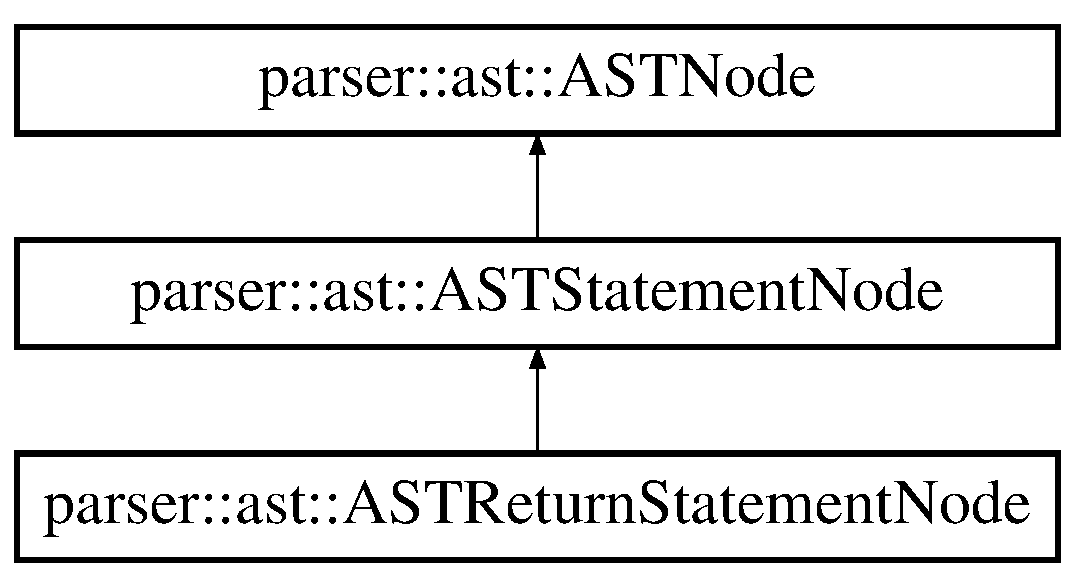
\includegraphics[height=3.000000cm]{dd/d96/classparser_1_1ast_1_1ASTReturnStatementNode}
\end{center}
\end{figure}
\subsection*{Public Member Functions}
\begin{DoxyCompactItemize}
\item 
\hyperlink{classparser_1_1ast_1_1ASTReturnStatementNode_aa88792926907901c21090c2ad0203209}{A\+S\+T\+Return\+Statement\+Node} (std\+::unique\+\_\+ptr$<$ \hyperlink{classparser_1_1ast_1_1ASTExprNode}{A\+S\+T\+Expr\+Node} $>$ \hyperlink{classparser_1_1ast_1_1ASTReturnStatementNode_af0ee45b3faee9a37d6a36f7670a586f1}{expr})
\item 
std\+::unique\+\_\+ptr$<$ \hyperlink{classparser_1_1ast_1_1ASTExprNode}{A\+S\+T\+Expr\+Node} $>$ \& \hyperlink{classparser_1_1ast_1_1ASTReturnStatementNode_a6e10c7499773278d36493d9a9545438a}{get\+Expr} ()
\item 
Statement\+Type \hyperlink{classparser_1_1ast_1_1ASTReturnStatementNode_a8e1fdae4c10f1e3349b244914e5117be}{get\+Statement\+Type} () override
\item 
void \hyperlink{classparser_1_1ast_1_1ASTReturnStatementNode_ac66c375bc67277468711fdec08e93b15}{accept} (\hyperlink{classvisitor_1_1Visitor}{visitor\+::\+Visitor} $\ast$visitor) override
\end{DoxyCompactItemize}
\subsection*{Protected Attributes}
\begin{DoxyCompactItemize}
\item 
\mbox{\Hypertarget{classparser_1_1ast_1_1ASTReturnStatementNode_af0ee45b3faee9a37d6a36f7670a586f1}\label{classparser_1_1ast_1_1ASTReturnStatementNode_af0ee45b3faee9a37d6a36f7670a586f1}} 
std\+::unique\+\_\+ptr$<$ \hyperlink{classparser_1_1ast_1_1ASTExprNode}{A\+S\+T\+Expr\+Node} $>$ \hyperlink{classparser_1_1ast_1_1ASTReturnStatementNode_af0ee45b3faee9a37d6a36f7670a586f1}{expr}
\begin{DoxyCompactList}\small\item\em The expression whose result will be returned. \end{DoxyCompactList}\end{DoxyCompactItemize}


\subsection{Detailed Description}
This class represents a node in the A\+ST that represents a {\ttfamily return} statement. 

\subsection{Constructor \& Destructor Documentation}
\mbox{\Hypertarget{classparser_1_1ast_1_1ASTReturnStatementNode_aa88792926907901c21090c2ad0203209}\label{classparser_1_1ast_1_1ASTReturnStatementNode_aa88792926907901c21090c2ad0203209}} 
\index{parser\+::ast\+::\+A\+S\+T\+Return\+Statement\+Node@{parser\+::ast\+::\+A\+S\+T\+Return\+Statement\+Node}!A\+S\+T\+Return\+Statement\+Node@{A\+S\+T\+Return\+Statement\+Node}}
\index{A\+S\+T\+Return\+Statement\+Node@{A\+S\+T\+Return\+Statement\+Node}!parser\+::ast\+::\+A\+S\+T\+Return\+Statement\+Node@{parser\+::ast\+::\+A\+S\+T\+Return\+Statement\+Node}}
\subsubsection{\texorpdfstring{A\+S\+T\+Return\+Statement\+Node()}{ASTReturnStatementNode()}}
{\footnotesize\ttfamily parser\+::ast\+::\+A\+S\+T\+Return\+Statement\+Node\+::\+A\+S\+T\+Return\+Statement\+Node (\begin{DoxyParamCaption}\item[{std\+::unique\+\_\+ptr$<$ \hyperlink{classparser_1_1ast_1_1ASTExprNode}{A\+S\+T\+Expr\+Node} $>$}]{expr }\end{DoxyParamCaption})}

The constructor for this class 
\begin{DoxyParams}{Parameters}
{\em expr} & The expression whose result will be returned \\
\hline
\end{DoxyParams}


\subsection{Member Function Documentation}
\mbox{\Hypertarget{classparser_1_1ast_1_1ASTReturnStatementNode_ac66c375bc67277468711fdec08e93b15}\label{classparser_1_1ast_1_1ASTReturnStatementNode_ac66c375bc67277468711fdec08e93b15}} 
\index{parser\+::ast\+::\+A\+S\+T\+Return\+Statement\+Node@{parser\+::ast\+::\+A\+S\+T\+Return\+Statement\+Node}!accept@{accept}}
\index{accept@{accept}!parser\+::ast\+::\+A\+S\+T\+Return\+Statement\+Node@{parser\+::ast\+::\+A\+S\+T\+Return\+Statement\+Node}}
\subsubsection{\texorpdfstring{accept()}{accept()}}
{\footnotesize\ttfamily void parser\+::ast\+::\+A\+S\+T\+Return\+Statement\+Node\+::accept (\begin{DoxyParamCaption}\item[{\hyperlink{classvisitor_1_1Visitor}{visitor\+::\+Visitor} $\ast$}]{visitor }\end{DoxyParamCaption})\hspace{0.3cm}{\ttfamily [override]}, {\ttfamily [virtual]}}

Accepts a visitor and calls the operation by invoking {\ttfamily visit(this)} 
\begin{DoxyParams}{Parameters}
{\em visitor} & the visitor to accept \\
\hline
\end{DoxyParams}


Implements \hyperlink{classparser_1_1ast_1_1ASTNode_a3ff84fdfdbbc5c39b70b4d04c22e7dc3}{parser\+::ast\+::\+A\+S\+T\+Node}.

\mbox{\Hypertarget{classparser_1_1ast_1_1ASTReturnStatementNode_a6e10c7499773278d36493d9a9545438a}\label{classparser_1_1ast_1_1ASTReturnStatementNode_a6e10c7499773278d36493d9a9545438a}} 
\index{parser\+::ast\+::\+A\+S\+T\+Return\+Statement\+Node@{parser\+::ast\+::\+A\+S\+T\+Return\+Statement\+Node}!get\+Expr@{get\+Expr}}
\index{get\+Expr@{get\+Expr}!parser\+::ast\+::\+A\+S\+T\+Return\+Statement\+Node@{parser\+::ast\+::\+A\+S\+T\+Return\+Statement\+Node}}
\subsubsection{\texorpdfstring{get\+Expr()}{getExpr()}}
{\footnotesize\ttfamily std\+::unique\+\_\+ptr$<$ \hyperlink{classparser_1_1ast_1_1ASTExprNode}{parser\+::ast\+::\+A\+S\+T\+Expr\+Node} $>$ \& parser\+::ast\+::\+A\+S\+T\+Return\+Statement\+Node\+::get\+Expr (\begin{DoxyParamCaption}{ }\end{DoxyParamCaption})}

\begin{DoxyReturn}{Returns}
The expression whose result will be returned 
\end{DoxyReturn}
\mbox{\Hypertarget{classparser_1_1ast_1_1ASTReturnStatementNode_a8e1fdae4c10f1e3349b244914e5117be}\label{classparser_1_1ast_1_1ASTReturnStatementNode_a8e1fdae4c10f1e3349b244914e5117be}} 
\index{parser\+::ast\+::\+A\+S\+T\+Return\+Statement\+Node@{parser\+::ast\+::\+A\+S\+T\+Return\+Statement\+Node}!get\+Statement\+Type@{get\+Statement\+Type}}
\index{get\+Statement\+Type@{get\+Statement\+Type}!parser\+::ast\+::\+A\+S\+T\+Return\+Statement\+Node@{parser\+::ast\+::\+A\+S\+T\+Return\+Statement\+Node}}
\subsubsection{\texorpdfstring{get\+Statement\+Type()}{getStatementType()}}
{\footnotesize\ttfamily parser\+::ast\+::\+Statement\+Type parser\+::ast\+::\+A\+S\+T\+Return\+Statement\+Node\+::get\+Statement\+Type (\begin{DoxyParamCaption}{ }\end{DoxyParamCaption})\hspace{0.3cm}{\ttfamily [override]}, {\ttfamily [virtual]}}

Virtual Method to return the statement type \begin{DoxyReturn}{Returns}
The statement type (instead of checking what class it\textquotesingle{}s an instance of) 
\end{DoxyReturn}


Implements \hyperlink{classparser_1_1ast_1_1ASTStatementNode_ac381d35d12f774a1bab0e209c5bfec1f}{parser\+::ast\+::\+A\+S\+T\+Statement\+Node}.



The documentation for this class was generated from the following files\+:\begin{DoxyCompactItemize}
\item 
parser/ast/statement/\hyperlink{ASTReturnStatementNode_8h}{A\+S\+T\+Return\+Statement\+Node.\+h}\item 
parser/ast/statement/A\+S\+T\+Return\+Statement\+Node.\+cpp\end{DoxyCompactItemize}

\hypertarget{classparser_1_1ast_1_1ASTSimpleExprNode}{}\section{parser\+:\+:ast\+:\+:A\+S\+T\+Simple\+Expr\+Node Class Reference}
\label{classparser_1_1ast_1_1ASTSimpleExprNode}\index{parser\+::ast\+::\+A\+S\+T\+Simple\+Expr\+Node@{parser\+::ast\+::\+A\+S\+T\+Simple\+Expr\+Node}}


{\ttfamily \#include $<$A\+S\+T\+Simple\+Expr\+Node.\+h$>$}

Inheritance diagram for parser\+:\+:ast\+:\+:A\+S\+T\+Simple\+Expr\+Node\+:\begin{figure}[H]
\begin{center}
\leavevmode
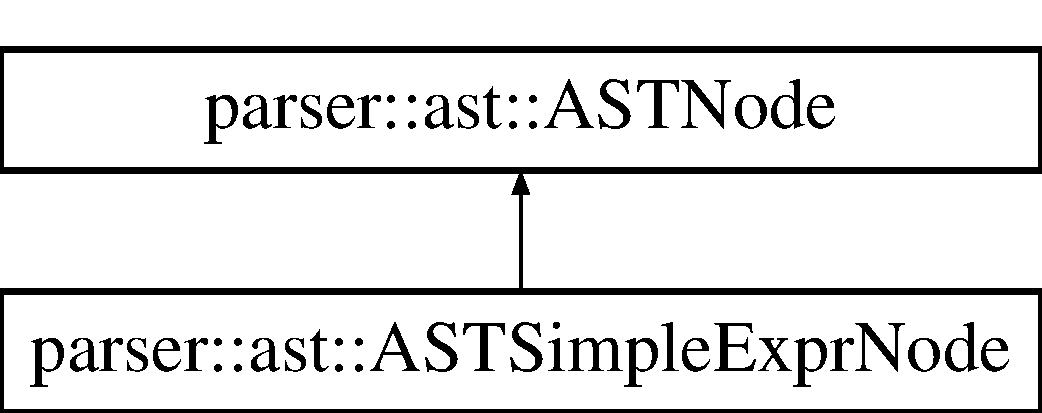
\includegraphics[height=2.000000cm]{d7/d5d/classparser_1_1ast_1_1ASTSimpleExprNode}
\end{center}
\end{figure}
\subsection*{Public Member Functions}
\begin{DoxyCompactItemize}
\item 
\hyperlink{classparser_1_1ast_1_1ASTSimpleExprNode_a882595847c545ef257df28c35ded464d}{A\+S\+T\+Simple\+Expr\+Node} (std\+::unique\+\_\+ptr$<$ \hyperlink{classparser_1_1ast_1_1ASTTermNode}{A\+S\+T\+Term\+Node} $>$ \hyperlink{classparser_1_1ast_1_1ASTSimpleExprNode_a3b8bc0ddeea8a027690259b2403c9f57}{left})
\item 
\hyperlink{classparser_1_1ast_1_1ASTSimpleExprNode_a2aa80137757c84581176e8e7e953811e}{A\+S\+T\+Simple\+Expr\+Node} (std\+::unique\+\_\+ptr$<$ \hyperlink{classparser_1_1ast_1_1ASTTermNode}{A\+S\+T\+Term\+Node} $>$ \hyperlink{classparser_1_1ast_1_1ASTSimpleExprNode_a3b8bc0ddeea8a027690259b2403c9f57}{left}, Additive\+Op \hyperlink{classparser_1_1ast_1_1ASTSimpleExprNode_a7b0f1134025df83440c78636f2c1dbd3}{add\+Op}, std\+::unique\+\_\+ptr$<$ \hyperlink{classparser_1_1ast_1_1ASTTermNode}{A\+S\+T\+Term\+Node} $>$ \hyperlink{classparser_1_1ast_1_1ASTSimpleExprNode_a3ca192d1465a7dfa33e7a1ece3084b54}{right})
\item 
std\+::unique\+\_\+ptr$<$ \hyperlink{classparser_1_1ast_1_1ASTTermNode}{A\+S\+T\+Term\+Node} $>$ \& \hyperlink{classparser_1_1ast_1_1ASTSimpleExprNode_a351105e2c9f21b40774b6e5949fdefb8}{get\+Left} ()
\item 
Additive\+Op \hyperlink{classparser_1_1ast_1_1ASTSimpleExprNode_a6081b08ef618cb72ae449d1e32913ae5}{get\+Add\+Op} ()
\item 
std\+::unique\+\_\+ptr$<$ \hyperlink{classparser_1_1ast_1_1ASTTermNode}{A\+S\+T\+Term\+Node} $>$ \& \hyperlink{classparser_1_1ast_1_1ASTSimpleExprNode_a08c175910e5c8ed18462c9919ff08343}{get\+Right} ()
\item 
std\+::string \hyperlink{classparser_1_1ast_1_1ASTSimpleExprNode_abf0a43427c061c963de936845ad3246d}{get\+Additive\+Operator\+String} ()
\item 
void \hyperlink{classparser_1_1ast_1_1ASTSimpleExprNode_a493a0e358cc89eb16f7a7ae9982d6527}{accept} (\hyperlink{classvisitor_1_1Visitor}{visitor\+::\+Visitor} $\ast$visitor) override
\end{DoxyCompactItemize}
\subsection*{Protected Attributes}
\begin{DoxyCompactItemize}
\item 
\mbox{\Hypertarget{classparser_1_1ast_1_1ASTSimpleExprNode_a3b8bc0ddeea8a027690259b2403c9f57}\label{classparser_1_1ast_1_1ASTSimpleExprNode_a3b8bc0ddeea8a027690259b2403c9f57}} 
std\+::unique\+\_\+ptr$<$ \hyperlink{classparser_1_1ast_1_1ASTTermNode}{A\+S\+T\+Term\+Node} $>$ \hyperlink{classparser_1_1ast_1_1ASTSimpleExprNode_a3b8bc0ddeea8a027690259b2403c9f57}{left}
\begin{DoxyCompactList}\small\item\em The left hand term of this expression (mandatory) \end{DoxyCompactList}\item 
\mbox{\Hypertarget{classparser_1_1ast_1_1ASTSimpleExprNode_a7b0f1134025df83440c78636f2c1dbd3}\label{classparser_1_1ast_1_1ASTSimpleExprNode_a7b0f1134025df83440c78636f2c1dbd3}} 
Additive\+Op \hyperlink{classparser_1_1ast_1_1ASTSimpleExprNode_a7b0f1134025df83440c78636f2c1dbd3}{add\+Op}
\begin{DoxyCompactList}\small\item\em The additive operator of this expression (mandatory if right hand side is present) \end{DoxyCompactList}\item 
\mbox{\Hypertarget{classparser_1_1ast_1_1ASTSimpleExprNode_a3ca192d1465a7dfa33e7a1ece3084b54}\label{classparser_1_1ast_1_1ASTSimpleExprNode_a3ca192d1465a7dfa33e7a1ece3084b54}} 
std\+::unique\+\_\+ptr$<$ \hyperlink{classparser_1_1ast_1_1ASTTermNode}{A\+S\+T\+Term\+Node} $>$ \hyperlink{classparser_1_1ast_1_1ASTSimpleExprNode_a3ca192d1465a7dfa33e7a1ece3084b54}{right}
\begin{DoxyCompactList}\small\item\em The right hand side of this expression (optional) \end{DoxyCompactList}\end{DoxyCompactItemize}


\subsection{Detailed Description}
Class representing a simple expression in the A\+ST 

\subsection{Constructor \& Destructor Documentation}
\mbox{\Hypertarget{classparser_1_1ast_1_1ASTSimpleExprNode_a882595847c545ef257df28c35ded464d}\label{classparser_1_1ast_1_1ASTSimpleExprNode_a882595847c545ef257df28c35ded464d}} 
\index{parser\+::ast\+::\+A\+S\+T\+Simple\+Expr\+Node@{parser\+::ast\+::\+A\+S\+T\+Simple\+Expr\+Node}!A\+S\+T\+Simple\+Expr\+Node@{A\+S\+T\+Simple\+Expr\+Node}}
\index{A\+S\+T\+Simple\+Expr\+Node@{A\+S\+T\+Simple\+Expr\+Node}!parser\+::ast\+::\+A\+S\+T\+Simple\+Expr\+Node@{parser\+::ast\+::\+A\+S\+T\+Simple\+Expr\+Node}}
\subsubsection{\texorpdfstring{A\+S\+T\+Simple\+Expr\+Node()}{ASTSimpleExprNode()}\hspace{0.1cm}{\footnotesize\ttfamily [1/2]}}
{\footnotesize\ttfamily parser\+::ast\+::\+A\+S\+T\+Simple\+Expr\+Node\+::\+A\+S\+T\+Simple\+Expr\+Node (\begin{DoxyParamCaption}\item[{std\+::unique\+\_\+ptr$<$ \hyperlink{classparser_1_1ast_1_1ASTTermNode}{A\+S\+T\+Term\+Node} $>$}]{left }\end{DoxyParamCaption})}

Constructor for when the simple expression is only made up of the left hand side 
\begin{DoxyParams}{Parameters}
{\em left} & The left hand side term of this simple expression \\
\hline
\end{DoxyParams}
\mbox{\Hypertarget{classparser_1_1ast_1_1ASTSimpleExprNode_a2aa80137757c84581176e8e7e953811e}\label{classparser_1_1ast_1_1ASTSimpleExprNode_a2aa80137757c84581176e8e7e953811e}} 
\index{parser\+::ast\+::\+A\+S\+T\+Simple\+Expr\+Node@{parser\+::ast\+::\+A\+S\+T\+Simple\+Expr\+Node}!A\+S\+T\+Simple\+Expr\+Node@{A\+S\+T\+Simple\+Expr\+Node}}
\index{A\+S\+T\+Simple\+Expr\+Node@{A\+S\+T\+Simple\+Expr\+Node}!parser\+::ast\+::\+A\+S\+T\+Simple\+Expr\+Node@{parser\+::ast\+::\+A\+S\+T\+Simple\+Expr\+Node}}
\subsubsection{\texorpdfstring{A\+S\+T\+Simple\+Expr\+Node()}{ASTSimpleExprNode()}\hspace{0.1cm}{\footnotesize\ttfamily [2/2]}}
{\footnotesize\ttfamily parser\+::ast\+::\+A\+S\+T\+Simple\+Expr\+Node\+::\+A\+S\+T\+Simple\+Expr\+Node (\begin{DoxyParamCaption}\item[{std\+::unique\+\_\+ptr$<$ \hyperlink{classparser_1_1ast_1_1ASTTermNode}{A\+S\+T\+Term\+Node} $>$}]{left,  }\item[{Additive\+Op}]{add\+Op,  }\item[{std\+::unique\+\_\+ptr$<$ \hyperlink{classparser_1_1ast_1_1ASTTermNode}{A\+S\+T\+Term\+Node} $>$}]{right }\end{DoxyParamCaption})}

Constructor for when the simple expression is made up of both sides 
\begin{DoxyParams}{Parameters}
{\em left} & The left hand side term of this simple expression \\
\hline
{\em add\+Op} & The additive operator for this simple expression. This can be one of\+:
\begin{DoxyItemize}
\item {\ttfamily A\+DD} \+: addition
\item {\ttfamily M\+I\+N\+US} \+: subtraction
\item {\ttfamily OR} \+: or 
\end{DoxyItemize}\\
\hline
{\em right} & The right hand side term of this simple expression. \\
\hline
\end{DoxyParams}


\subsection{Member Function Documentation}
\mbox{\Hypertarget{classparser_1_1ast_1_1ASTSimpleExprNode_a493a0e358cc89eb16f7a7ae9982d6527}\label{classparser_1_1ast_1_1ASTSimpleExprNode_a493a0e358cc89eb16f7a7ae9982d6527}} 
\index{parser\+::ast\+::\+A\+S\+T\+Simple\+Expr\+Node@{parser\+::ast\+::\+A\+S\+T\+Simple\+Expr\+Node}!accept@{accept}}
\index{accept@{accept}!parser\+::ast\+::\+A\+S\+T\+Simple\+Expr\+Node@{parser\+::ast\+::\+A\+S\+T\+Simple\+Expr\+Node}}
\subsubsection{\texorpdfstring{accept()}{accept()}}
{\footnotesize\ttfamily void parser\+::ast\+::\+A\+S\+T\+Simple\+Expr\+Node\+::accept (\begin{DoxyParamCaption}\item[{\hyperlink{classvisitor_1_1Visitor}{visitor\+::\+Visitor} $\ast$}]{visitor }\end{DoxyParamCaption})\hspace{0.3cm}{\ttfamily [override]}, {\ttfamily [virtual]}}

Accepts a visitor and calls the operation by invoking {\ttfamily visit(this)} 
\begin{DoxyParams}{Parameters}
{\em visitor} & the visitor to accept \\
\hline
\end{DoxyParams}


Implements \hyperlink{classparser_1_1ast_1_1ASTNode_a3ff84fdfdbbc5c39b70b4d04c22e7dc3}{parser\+::ast\+::\+A\+S\+T\+Node}.

\mbox{\Hypertarget{classparser_1_1ast_1_1ASTSimpleExprNode_abf0a43427c061c963de936845ad3246d}\label{classparser_1_1ast_1_1ASTSimpleExprNode_abf0a43427c061c963de936845ad3246d}} 
\index{parser\+::ast\+::\+A\+S\+T\+Simple\+Expr\+Node@{parser\+::ast\+::\+A\+S\+T\+Simple\+Expr\+Node}!get\+Additive\+Operator\+String@{get\+Additive\+Operator\+String}}
\index{get\+Additive\+Operator\+String@{get\+Additive\+Operator\+String}!parser\+::ast\+::\+A\+S\+T\+Simple\+Expr\+Node@{parser\+::ast\+::\+A\+S\+T\+Simple\+Expr\+Node}}
\subsubsection{\texorpdfstring{get\+Additive\+Operator\+String()}{getAdditiveOperatorString()}}
{\footnotesize\ttfamily std\+::string parser\+::ast\+::\+A\+S\+T\+Simple\+Expr\+Node\+::get\+Additive\+Operator\+String (\begin{DoxyParamCaption}{ }\end{DoxyParamCaption})}


\begin{DoxyParams}{Parameters}
{\em ad\+Op} & The additive operator to convert to a string \\
\hline
\end{DoxyParams}
\begin{DoxyReturn}{Returns}
String representing the additive operator 
\end{DoxyReturn}
\mbox{\Hypertarget{classparser_1_1ast_1_1ASTSimpleExprNode_a6081b08ef618cb72ae449d1e32913ae5}\label{classparser_1_1ast_1_1ASTSimpleExprNode_a6081b08ef618cb72ae449d1e32913ae5}} 
\index{parser\+::ast\+::\+A\+S\+T\+Simple\+Expr\+Node@{parser\+::ast\+::\+A\+S\+T\+Simple\+Expr\+Node}!get\+Add\+Op@{get\+Add\+Op}}
\index{get\+Add\+Op@{get\+Add\+Op}!parser\+::ast\+::\+A\+S\+T\+Simple\+Expr\+Node@{parser\+::ast\+::\+A\+S\+T\+Simple\+Expr\+Node}}
\subsubsection{\texorpdfstring{get\+Add\+Op()}{getAddOp()}}
{\footnotesize\ttfamily parser\+::ast\+::\+Additive\+Op parser\+::ast\+::\+A\+S\+T\+Simple\+Expr\+Node\+::get\+Add\+Op (\begin{DoxyParamCaption}{ }\end{DoxyParamCaption})}

\begin{DoxyReturn}{Returns}
Additive Operator type of this expression 
\end{DoxyReturn}
\mbox{\Hypertarget{classparser_1_1ast_1_1ASTSimpleExprNode_a351105e2c9f21b40774b6e5949fdefb8}\label{classparser_1_1ast_1_1ASTSimpleExprNode_a351105e2c9f21b40774b6e5949fdefb8}} 
\index{parser\+::ast\+::\+A\+S\+T\+Simple\+Expr\+Node@{parser\+::ast\+::\+A\+S\+T\+Simple\+Expr\+Node}!get\+Left@{get\+Left}}
\index{get\+Left@{get\+Left}!parser\+::ast\+::\+A\+S\+T\+Simple\+Expr\+Node@{parser\+::ast\+::\+A\+S\+T\+Simple\+Expr\+Node}}
\subsubsection{\texorpdfstring{get\+Left()}{getLeft()}}
{\footnotesize\ttfamily std\+::unique\+\_\+ptr$<$ \hyperlink{classparser_1_1ast_1_1ASTTermNode}{parser\+::ast\+::\+A\+S\+T\+Term\+Node} $>$ \& parser\+::ast\+::\+A\+S\+T\+Simple\+Expr\+Node\+::get\+Left (\begin{DoxyParamCaption}{ }\end{DoxyParamCaption})}

\begin{DoxyReturn}{Returns}
Pointer to the left hand side of the simple expression 
\end{DoxyReturn}
\mbox{\Hypertarget{classparser_1_1ast_1_1ASTSimpleExprNode_a08c175910e5c8ed18462c9919ff08343}\label{classparser_1_1ast_1_1ASTSimpleExprNode_a08c175910e5c8ed18462c9919ff08343}} 
\index{parser\+::ast\+::\+A\+S\+T\+Simple\+Expr\+Node@{parser\+::ast\+::\+A\+S\+T\+Simple\+Expr\+Node}!get\+Right@{get\+Right}}
\index{get\+Right@{get\+Right}!parser\+::ast\+::\+A\+S\+T\+Simple\+Expr\+Node@{parser\+::ast\+::\+A\+S\+T\+Simple\+Expr\+Node}}
\subsubsection{\texorpdfstring{get\+Right()}{getRight()}}
{\footnotesize\ttfamily std\+::unique\+\_\+ptr$<$ \hyperlink{classparser_1_1ast_1_1ASTTermNode}{parser\+::ast\+::\+A\+S\+T\+Term\+Node} $>$ \& parser\+::ast\+::\+A\+S\+T\+Simple\+Expr\+Node\+::get\+Right (\begin{DoxyParamCaption}{ }\end{DoxyParamCaption})}

\begin{DoxyReturn}{Returns}
Pointer to the right hand side of the simple expression 
\end{DoxyReturn}


The documentation for this class was generated from the following files\+:\begin{DoxyCompactItemize}
\item 
parser/ast/expression/A\+S\+T\+Simple\+Expr\+Node.\+h\item 
parser/ast/expression/A\+S\+T\+Simple\+Expr\+Node.\+cpp\end{DoxyCompactItemize}

\hypertarget{classparser_1_1ast_1_1ASTStatementNode}{}\section{parser\+:\+:ast\+:\+:A\+S\+T\+Statement\+Node Class Reference}
\label{classparser_1_1ast_1_1ASTStatementNode}\index{parser\+::ast\+::\+A\+S\+T\+Statement\+Node@{parser\+::ast\+::\+A\+S\+T\+Statement\+Node}}
Inheritance diagram for parser\+:\+:ast\+:\+:A\+S\+T\+Statement\+Node\+:\begin{figure}[H]
\begin{center}
\leavevmode
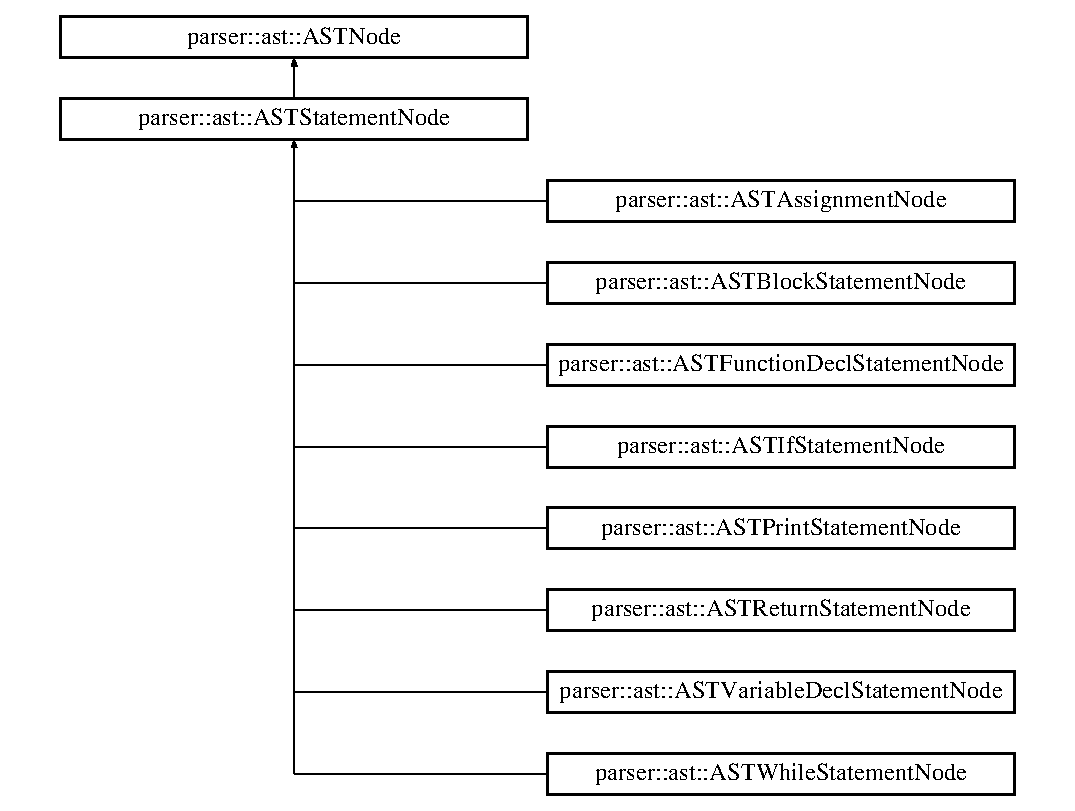
\includegraphics[height=10.000000cm]{de/dbf/classparser_1_1ast_1_1ASTStatementNode}
\end{center}
\end{figure}
\subsection*{Public Member Functions}
\begin{DoxyCompactItemize}
\item 
virtual Statement\+Type \hyperlink{classparser_1_1ast_1_1ASTStatementNode_ac381d35d12f774a1bab0e209c5bfec1f}{get\+Statement\+Type} ()=0
\end{DoxyCompactItemize}


\subsection{Member Function Documentation}
\mbox{\Hypertarget{classparser_1_1ast_1_1ASTStatementNode_ac381d35d12f774a1bab0e209c5bfec1f}\label{classparser_1_1ast_1_1ASTStatementNode_ac381d35d12f774a1bab0e209c5bfec1f}} 
\index{parser\+::ast\+::\+A\+S\+T\+Statement\+Node@{parser\+::ast\+::\+A\+S\+T\+Statement\+Node}!get\+Statement\+Type@{get\+Statement\+Type}}
\index{get\+Statement\+Type@{get\+Statement\+Type}!parser\+::ast\+::\+A\+S\+T\+Statement\+Node@{parser\+::ast\+::\+A\+S\+T\+Statement\+Node}}
\subsubsection{\texorpdfstring{get\+Statement\+Type()}{getStatementType()}}
{\footnotesize\ttfamily virtual Statement\+Type parser\+::ast\+::\+A\+S\+T\+Statement\+Node\+::get\+Statement\+Type (\begin{DoxyParamCaption}{ }\end{DoxyParamCaption})\hspace{0.3cm}{\ttfamily [pure virtual]}}

Virtual Method to return the statement type \begin{DoxyReturn}{Returns}
The statement type (instead of checking what class it\textquotesingle{}s an instance of) 
\end{DoxyReturn}


Implemented in \hyperlink{classparser_1_1ast_1_1ASTVariableDeclStatementNode_a273b2c22a426022608813603ddfd820b}{parser\+::ast\+::\+A\+S\+T\+Variable\+Decl\+Statement\+Node}, \hyperlink{classparser_1_1ast_1_1ASTFunctionDeclStatementNode_af951f3f6b2b47831a252bafe3dcb2a1f}{parser\+::ast\+::\+A\+S\+T\+Function\+Decl\+Statement\+Node}, \hyperlink{classparser_1_1ast_1_1ASTIfStatementNode_aebe9139e5ee81c851aa01fd292635562}{parser\+::ast\+::\+A\+S\+T\+If\+Statement\+Node}, \hyperlink{classparser_1_1ast_1_1ASTAssignmentNode_ad53e33c7aa72d26b67e38699bdac2e32}{parser\+::ast\+::\+A\+S\+T\+Assignment\+Node}, \hyperlink{classparser_1_1ast_1_1ASTWhileStatementNode_a47ad4212e8bae1bbe602918044e39cd8}{parser\+::ast\+::\+A\+S\+T\+While\+Statement\+Node}, \hyperlink{classparser_1_1ast_1_1ASTReturnStatementNode_a8e1fdae4c10f1e3349b244914e5117be}{parser\+::ast\+::\+A\+S\+T\+Return\+Statement\+Node}, \hyperlink{classparser_1_1ast_1_1ASTBlockStatementNode_aec80a6d582f0b9691dbd33d0d5ecb975}{parser\+::ast\+::\+A\+S\+T\+Block\+Statement\+Node}, and \hyperlink{classparser_1_1ast_1_1ASTPrintStatementNode_a9526c5de33100e05f1ccba710c0a9a34}{parser\+::ast\+::\+A\+S\+T\+Print\+Statement\+Node}.



The documentation for this class was generated from the following file\+:\begin{DoxyCompactItemize}
\item 
parser/ast/A\+S\+T\+Statement\+Node.\+h\end{DoxyCompactItemize}

\hypertarget{classparser_1_1ast_1_1ASTSubExpression}{}\section{parser\+:\+:ast\+:\+:A\+S\+T\+Sub\+Expression Class Reference}
\label{classparser_1_1ast_1_1ASTSubExpression}\index{parser\+::ast\+::\+A\+S\+T\+Sub\+Expression@{parser\+::ast\+::\+A\+S\+T\+Sub\+Expression}}


{\ttfamily \#include $<$A\+S\+T\+Sub\+Expression.\+h$>$}

Inheritance diagram for parser\+:\+:ast\+:\+:A\+S\+T\+Sub\+Expression\+:\begin{figure}[H]
\begin{center}
\leavevmode
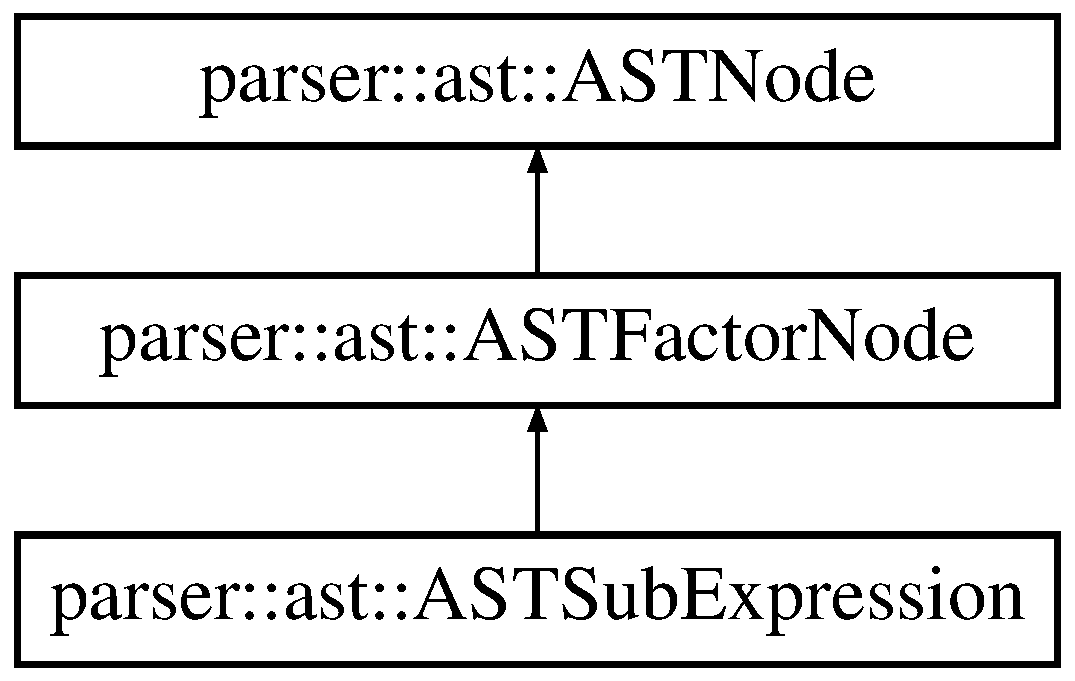
\includegraphics[height=3.000000cm]{d9/d21/classparser_1_1ast_1_1ASTSubExpression}
\end{center}
\end{figure}
\subsection*{Public Member Functions}
\begin{DoxyCompactItemize}
\item 
\hyperlink{classparser_1_1ast_1_1ASTSubExpression_ad3c1de057f3edff4ce3e30d449cf0654}{A\+S\+T\+Sub\+Expression} (std\+::unique\+\_\+ptr$<$ \hyperlink{classparser_1_1ast_1_1ASTExprNode}{A\+S\+T\+Expr\+Node} $>$ \hyperlink{classparser_1_1ast_1_1ASTSubExpression_abccfde1fa38ce0cdd3bc60993ae0e493}{expr})
\item 
const std\+::unique\+\_\+ptr$<$ \hyperlink{classparser_1_1ast_1_1ASTExprNode}{A\+S\+T\+Expr\+Node} $>$ \& \hyperlink{classparser_1_1ast_1_1ASTSubExpression_ab25ef09e54236f4e10e944b09cb23935}{get\+Expr} () const
\item 
\hyperlink{ASTFactorNode_8h_afbe2fcc03ef15b74a0c1ed1cda7ab0e8}{Factor\+Type} \hyperlink{classparser_1_1ast_1_1ASTSubExpression_a0a7ade91b1cce64eacfb9b5f6167db3f}{get\+Factor\+Type} () override
\item 
void \hyperlink{classparser_1_1ast_1_1ASTSubExpression_a684e39e8385690e9bade65731ba5803b}{accept} (\hyperlink{classvisitor_1_1Visitor}{visitor\+::\+Visitor} $\ast$visitor) override
\end{DoxyCompactItemize}
\subsection*{Protected Attributes}
\begin{DoxyCompactItemize}
\item 
\mbox{\Hypertarget{classparser_1_1ast_1_1ASTSubExpression_abccfde1fa38ce0cdd3bc60993ae0e493}\label{classparser_1_1ast_1_1ASTSubExpression_abccfde1fa38ce0cdd3bc60993ae0e493}} 
std\+::unique\+\_\+ptr$<$ \hyperlink{classparser_1_1ast_1_1ASTExprNode}{A\+S\+T\+Expr\+Node} $>$ \hyperlink{classparser_1_1ast_1_1ASTSubExpression_abccfde1fa38ce0cdd3bc60993ae0e493}{expr}
\begin{DoxyCompactList}\small\item\em The expression itself. \end{DoxyCompactList}\end{DoxyCompactItemize}


\subsection{Detailed Description}
Class represneting a sub-\/expression in the A\+ST 

\subsection{Constructor \& Destructor Documentation}
\mbox{\Hypertarget{classparser_1_1ast_1_1ASTSubExpression_ad3c1de057f3edff4ce3e30d449cf0654}\label{classparser_1_1ast_1_1ASTSubExpression_ad3c1de057f3edff4ce3e30d449cf0654}} 
\index{parser\+::ast\+::\+A\+S\+T\+Sub\+Expression@{parser\+::ast\+::\+A\+S\+T\+Sub\+Expression}!A\+S\+T\+Sub\+Expression@{A\+S\+T\+Sub\+Expression}}
\index{A\+S\+T\+Sub\+Expression@{A\+S\+T\+Sub\+Expression}!parser\+::ast\+::\+A\+S\+T\+Sub\+Expression@{parser\+::ast\+::\+A\+S\+T\+Sub\+Expression}}
\subsubsection{\texorpdfstring{A\+S\+T\+Sub\+Expression()}{ASTSubExpression()}}
{\footnotesize\ttfamily parser\+::ast\+::\+A\+S\+T\+Sub\+Expression\+::\+A\+S\+T\+Sub\+Expression (\begin{DoxyParamCaption}\item[{std\+::unique\+\_\+ptr$<$ \hyperlink{classparser_1_1ast_1_1ASTExprNode}{A\+S\+T\+Expr\+Node} $>$}]{expr }\end{DoxyParamCaption})}

Constructor for this sub-\/expression 
\begin{DoxyParams}{Parameters}
{\em expr} & pointer to the expression of this sub-\/expression \\
\hline
\end{DoxyParams}


\subsection{Member Function Documentation}
\mbox{\Hypertarget{classparser_1_1ast_1_1ASTSubExpression_a684e39e8385690e9bade65731ba5803b}\label{classparser_1_1ast_1_1ASTSubExpression_a684e39e8385690e9bade65731ba5803b}} 
\index{parser\+::ast\+::\+A\+S\+T\+Sub\+Expression@{parser\+::ast\+::\+A\+S\+T\+Sub\+Expression}!accept@{accept}}
\index{accept@{accept}!parser\+::ast\+::\+A\+S\+T\+Sub\+Expression@{parser\+::ast\+::\+A\+S\+T\+Sub\+Expression}}
\subsubsection{\texorpdfstring{accept()}{accept()}}
{\footnotesize\ttfamily void parser\+::ast\+::\+A\+S\+T\+Sub\+Expression\+::accept (\begin{DoxyParamCaption}\item[{\hyperlink{classvisitor_1_1Visitor}{visitor\+::\+Visitor} $\ast$}]{visitor }\end{DoxyParamCaption})\hspace{0.3cm}{\ttfamily [override]}, {\ttfamily [virtual]}}

Accepts a visitor and calls the operation by invoking {\ttfamily visit(this)} 
\begin{DoxyParams}{Parameters}
{\em visitor} & the visitor to accept \\
\hline
\end{DoxyParams}


Implements \hyperlink{classparser_1_1ast_1_1ASTNode_a3ff84fdfdbbc5c39b70b4d04c22e7dc3}{parser\+::ast\+::\+A\+S\+T\+Node}.

\mbox{\Hypertarget{classparser_1_1ast_1_1ASTSubExpression_ab25ef09e54236f4e10e944b09cb23935}\label{classparser_1_1ast_1_1ASTSubExpression_ab25ef09e54236f4e10e944b09cb23935}} 
\index{parser\+::ast\+::\+A\+S\+T\+Sub\+Expression@{parser\+::ast\+::\+A\+S\+T\+Sub\+Expression}!get\+Expr@{get\+Expr}}
\index{get\+Expr@{get\+Expr}!parser\+::ast\+::\+A\+S\+T\+Sub\+Expression@{parser\+::ast\+::\+A\+S\+T\+Sub\+Expression}}
\subsubsection{\texorpdfstring{get\+Expr()}{getExpr()}}
{\footnotesize\ttfamily const std\+::unique\+\_\+ptr$<$ \hyperlink{classparser_1_1ast_1_1ASTExprNode}{parser\+::ast\+::\+A\+S\+T\+Expr\+Node} $>$ \& parser\+::ast\+::\+A\+S\+T\+Sub\+Expression\+::get\+Expr (\begin{DoxyParamCaption}{ }\end{DoxyParamCaption}) const}

\begin{DoxyReturn}{Returns}
pointer to the expression of this sub-\/expression 
\end{DoxyReturn}
\mbox{\Hypertarget{classparser_1_1ast_1_1ASTSubExpression_a0a7ade91b1cce64eacfb9b5f6167db3f}\label{classparser_1_1ast_1_1ASTSubExpression_a0a7ade91b1cce64eacfb9b5f6167db3f}} 
\index{parser\+::ast\+::\+A\+S\+T\+Sub\+Expression@{parser\+::ast\+::\+A\+S\+T\+Sub\+Expression}!get\+Factor\+Type@{get\+Factor\+Type}}
\index{get\+Factor\+Type@{get\+Factor\+Type}!parser\+::ast\+::\+A\+S\+T\+Sub\+Expression@{parser\+::ast\+::\+A\+S\+T\+Sub\+Expression}}
\subsubsection{\texorpdfstring{get\+Factor\+Type()}{getFactorType()}}
{\footnotesize\ttfamily \hyperlink{ASTFactorNode_8h_afbe2fcc03ef15b74a0c1ed1cda7ab0e8}{parser\+::ast\+::\+Factor\+Type} parser\+::ast\+::\+A\+S\+T\+Sub\+Expression\+::get\+Factor\+Type (\begin{DoxyParamCaption}{ }\end{DoxyParamCaption})\hspace{0.3cm}{\ttfamily [override]}, {\ttfamily [virtual]}}

\begin{DoxyReturn}{Returns}
The type of factor this is. Use instead of checking the class type. 
\end{DoxyReturn}


Implements \hyperlink{classparser_1_1ast_1_1ASTFactorNode_a13eea7f949c0055dea0a9d7b715f16a8}{parser\+::ast\+::\+A\+S\+T\+Factor\+Node}.



The documentation for this class was generated from the following files\+:\begin{DoxyCompactItemize}
\item 
parser/ast/expression/factor/\hyperlink{ASTSubExpression_8h}{A\+S\+T\+Sub\+Expression.\+h}\item 
parser/ast/expression/factor/\hyperlink{ASTSubExpression_8cpp}{A\+S\+T\+Sub\+Expression.\+cpp}\end{DoxyCompactItemize}

\hypertarget{classparser_1_1ast_1_1ASTTermNode}{}\section{parser\+:\+:ast\+:\+:A\+S\+T\+Term\+Node Class Reference}
\label{classparser_1_1ast_1_1ASTTermNode}\index{parser\+::ast\+::\+A\+S\+T\+Term\+Node@{parser\+::ast\+::\+A\+S\+T\+Term\+Node}}


{\ttfamily \#include $<$A\+S\+T\+Term\+Node.\+h$>$}

Inheritance diagram for parser\+:\+:ast\+:\+:A\+S\+T\+Term\+Node\+:\begin{figure}[H]
\begin{center}
\leavevmode
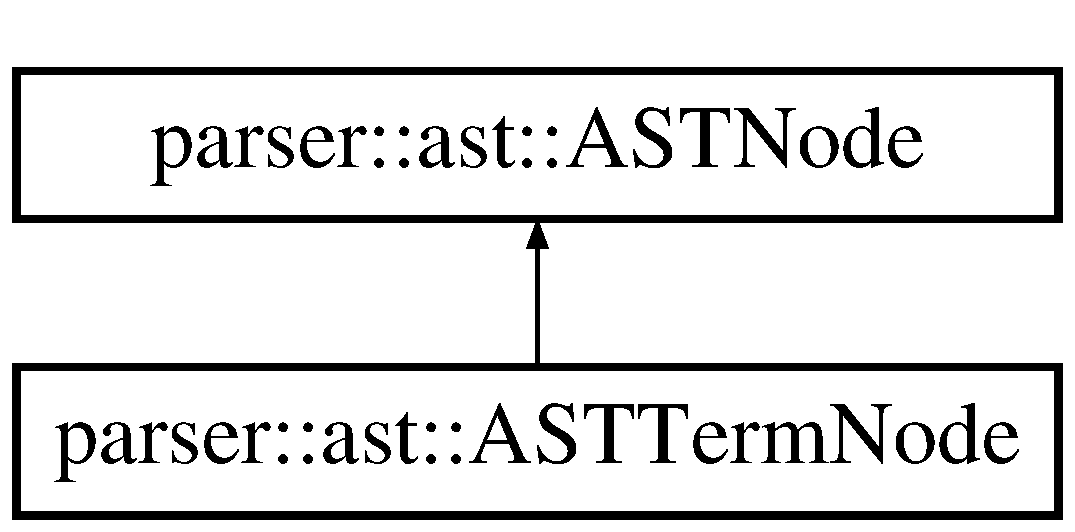
\includegraphics[height=2.000000cm]{de/d23/classparser_1_1ast_1_1ASTTermNode}
\end{center}
\end{figure}
\subsection*{Public Member Functions}
\begin{DoxyCompactItemize}
\item 
\hyperlink{classparser_1_1ast_1_1ASTTermNode_ab37b86959cf1761c460ca678dc44aa3e}{A\+S\+T\+Term\+Node} (std\+::unique\+\_\+ptr$<$ \hyperlink{classparser_1_1ast_1_1ASTFactorNode}{A\+S\+T\+Factor\+Node} $>$ \hyperlink{classparser_1_1ast_1_1ASTTermNode_a268410bee7baf3e6dd0a1fa64fc0c0e2}{left}, \hyperlink{ASTTermNode_8h_a56419c32f44e139982c327d8375a27a7}{Multiplicative\+Op} \hyperlink{classparser_1_1ast_1_1ASTTermNode_a5fca22b04d30310ff59616a7e0863a54}{op}, std\+::unique\+\_\+ptr$<$ \hyperlink{classparser_1_1ast_1_1ASTFactorNode}{A\+S\+T\+Factor\+Node} $>$ \hyperlink{classparser_1_1ast_1_1ASTTermNode_a339078e4e969f51d2da01a39585db008}{right})
\item 
\hyperlink{classparser_1_1ast_1_1ASTTermNode_ac8e1cb1e76e14a3f472ea58e27d079be}{A\+S\+T\+Term\+Node} (std\+::unique\+\_\+ptr$<$ \hyperlink{classparser_1_1ast_1_1ASTFactorNode}{A\+S\+T\+Factor\+Node} $>$ \hyperlink{classparser_1_1ast_1_1ASTTermNode_a268410bee7baf3e6dd0a1fa64fc0c0e2}{left})
\item 
const std\+::unique\+\_\+ptr$<$ \hyperlink{classparser_1_1ast_1_1ASTFactorNode}{A\+S\+T\+Factor\+Node} $>$ \& \hyperlink{classparser_1_1ast_1_1ASTTermNode_a33fd3c6c4e20f282adac752fa222d569}{get\+Left} () const
\item 
\hyperlink{ASTTermNode_8h_a56419c32f44e139982c327d8375a27a7}{Multiplicative\+Op} \hyperlink{classparser_1_1ast_1_1ASTTermNode_a8216196b573296bb0a0bee30a908a9af}{get\+Op} () const
\item 
const std\+::unique\+\_\+ptr$<$ \hyperlink{classparser_1_1ast_1_1ASTFactorNode}{A\+S\+T\+Factor\+Node} $>$ \& \hyperlink{classparser_1_1ast_1_1ASTTermNode_aa7e15b30a84f8afcd75f85c354103ca0}{get\+Right} () const
\item 
\mbox{\Hypertarget{classparser_1_1ast_1_1ASTTermNode_a1e4ede7d3314cc5b5934f7754364acd9}\label{classparser_1_1ast_1_1ASTTermNode_a1e4ede7d3314cc5b5934f7754364acd9}} 
const std\+::string {\bfseries get\+Mutliplicative\+Op\+String} () const
\item 
void \hyperlink{classparser_1_1ast_1_1ASTTermNode_a4937651cff0fac499c76f8f38fa4795d}{accept} (\hyperlink{classvisitor_1_1Visitor}{visitor\+::\+Visitor} $\ast$visitor) override
\end{DoxyCompactItemize}
\subsection*{Protected Attributes}
\begin{DoxyCompactItemize}
\item 
\mbox{\Hypertarget{classparser_1_1ast_1_1ASTTermNode_a268410bee7baf3e6dd0a1fa64fc0c0e2}\label{classparser_1_1ast_1_1ASTTermNode_a268410bee7baf3e6dd0a1fa64fc0c0e2}} 
std\+::unique\+\_\+ptr$<$ \hyperlink{classparser_1_1ast_1_1ASTFactorNode}{A\+S\+T\+Factor\+Node} $>$ \hyperlink{classparser_1_1ast_1_1ASTTermNode_a268410bee7baf3e6dd0a1fa64fc0c0e2}{left}
\begin{DoxyCompactList}\small\item\em The left hand side factor of this term. \end{DoxyCompactList}\item 
\mbox{\Hypertarget{classparser_1_1ast_1_1ASTTermNode_a5fca22b04d30310ff59616a7e0863a54}\label{classparser_1_1ast_1_1ASTTermNode_a5fca22b04d30310ff59616a7e0863a54}} 
\hyperlink{ASTTermNode_8h_a56419c32f44e139982c327d8375a27a7}{Multiplicative\+Op} \hyperlink{classparser_1_1ast_1_1ASTTermNode_a5fca22b04d30310ff59616a7e0863a54}{op}
\begin{DoxyCompactList}\small\item\em The multiplicative operator of this term. Mandatory if right is not null. \end{DoxyCompactList}\item 
\mbox{\Hypertarget{classparser_1_1ast_1_1ASTTermNode_a339078e4e969f51d2da01a39585db008}\label{classparser_1_1ast_1_1ASTTermNode_a339078e4e969f51d2da01a39585db008}} 
std\+::unique\+\_\+ptr$<$ \hyperlink{classparser_1_1ast_1_1ASTFactorNode}{A\+S\+T\+Factor\+Node} $>$ \hyperlink{classparser_1_1ast_1_1ASTTermNode_a339078e4e969f51d2da01a39585db008}{right}
\begin{DoxyCompactList}\small\item\em The right hand side factor of this term. \end{DoxyCompactList}\end{DoxyCompactItemize}


\subsection{Detailed Description}
Class representing a Term node in the A\+ST 

\subsection{Constructor \& Destructor Documentation}
\mbox{\Hypertarget{classparser_1_1ast_1_1ASTTermNode_ab37b86959cf1761c460ca678dc44aa3e}\label{classparser_1_1ast_1_1ASTTermNode_ab37b86959cf1761c460ca678dc44aa3e}} 
\index{parser\+::ast\+::\+A\+S\+T\+Term\+Node@{parser\+::ast\+::\+A\+S\+T\+Term\+Node}!A\+S\+T\+Term\+Node@{A\+S\+T\+Term\+Node}}
\index{A\+S\+T\+Term\+Node@{A\+S\+T\+Term\+Node}!parser\+::ast\+::\+A\+S\+T\+Term\+Node@{parser\+::ast\+::\+A\+S\+T\+Term\+Node}}
\subsubsection{\texorpdfstring{A\+S\+T\+Term\+Node()}{ASTTermNode()}\hspace{0.1cm}{\footnotesize\ttfamily [1/2]}}
{\footnotesize\ttfamily parser\+::ast\+::\+A\+S\+T\+Term\+Node\+::\+A\+S\+T\+Term\+Node (\begin{DoxyParamCaption}\item[{std\+::unique\+\_\+ptr$<$ \hyperlink{classparser_1_1ast_1_1ASTFactorNode}{A\+S\+T\+Factor\+Node} $>$}]{left,  }\item[{\hyperlink{ASTTermNode_8h_a56419c32f44e139982c327d8375a27a7}{Multiplicative\+Op}}]{op,  }\item[{std\+::unique\+\_\+ptr$<$ \hyperlink{classparser_1_1ast_1_1ASTFactorNode}{A\+S\+T\+Factor\+Node} $>$}]{right }\end{DoxyParamCaption})}

Constructor when this Term has 2 factors (left hand side and right hand side) 
\begin{DoxyParams}{Parameters}
{\em left} & The left hand side of this term \\
\hline
{\em op} & The multiplicative operator to apply between the factors \\
\hline
{\em right} & The right hand side of this term \\
\hline
\end{DoxyParams}
\mbox{\Hypertarget{classparser_1_1ast_1_1ASTTermNode_ac8e1cb1e76e14a3f472ea58e27d079be}\label{classparser_1_1ast_1_1ASTTermNode_ac8e1cb1e76e14a3f472ea58e27d079be}} 
\index{parser\+::ast\+::\+A\+S\+T\+Term\+Node@{parser\+::ast\+::\+A\+S\+T\+Term\+Node}!A\+S\+T\+Term\+Node@{A\+S\+T\+Term\+Node}}
\index{A\+S\+T\+Term\+Node@{A\+S\+T\+Term\+Node}!parser\+::ast\+::\+A\+S\+T\+Term\+Node@{parser\+::ast\+::\+A\+S\+T\+Term\+Node}}
\subsubsection{\texorpdfstring{A\+S\+T\+Term\+Node()}{ASTTermNode()}\hspace{0.1cm}{\footnotesize\ttfamily [2/2]}}
{\footnotesize\ttfamily parser\+::ast\+::\+A\+S\+T\+Term\+Node\+::\+A\+S\+T\+Term\+Node (\begin{DoxyParamCaption}\item[{std\+::unique\+\_\+ptr$<$ \hyperlink{classparser_1_1ast_1_1ASTFactorNode}{A\+S\+T\+Factor\+Node} $>$}]{left }\end{DoxyParamCaption})}

Constructor when this term has only 1 factor 
\begin{DoxyParams}{Parameters}
{\em left} & The factor of this term \\
\hline
\end{DoxyParams}


\subsection{Member Function Documentation}
\mbox{\Hypertarget{classparser_1_1ast_1_1ASTTermNode_a4937651cff0fac499c76f8f38fa4795d}\label{classparser_1_1ast_1_1ASTTermNode_a4937651cff0fac499c76f8f38fa4795d}} 
\index{parser\+::ast\+::\+A\+S\+T\+Term\+Node@{parser\+::ast\+::\+A\+S\+T\+Term\+Node}!accept@{accept}}
\index{accept@{accept}!parser\+::ast\+::\+A\+S\+T\+Term\+Node@{parser\+::ast\+::\+A\+S\+T\+Term\+Node}}
\subsubsection{\texorpdfstring{accept()}{accept()}}
{\footnotesize\ttfamily void parser\+::ast\+::\+A\+S\+T\+Term\+Node\+::accept (\begin{DoxyParamCaption}\item[{\hyperlink{classvisitor_1_1Visitor}{visitor\+::\+Visitor} $\ast$}]{visitor }\end{DoxyParamCaption})\hspace{0.3cm}{\ttfamily [override]}, {\ttfamily [virtual]}}

Accepts a visitor and calls the operation by invoking {\ttfamily visit(this)} 
\begin{DoxyParams}{Parameters}
{\em visitor} & the visitor to accept \\
\hline
\end{DoxyParams}


Implements \hyperlink{classparser_1_1ast_1_1ASTNode_a3ff84fdfdbbc5c39b70b4d04c22e7dc3}{parser\+::ast\+::\+A\+S\+T\+Node}.

\mbox{\Hypertarget{classparser_1_1ast_1_1ASTTermNode_a33fd3c6c4e20f282adac752fa222d569}\label{classparser_1_1ast_1_1ASTTermNode_a33fd3c6c4e20f282adac752fa222d569}} 
\index{parser\+::ast\+::\+A\+S\+T\+Term\+Node@{parser\+::ast\+::\+A\+S\+T\+Term\+Node}!get\+Left@{get\+Left}}
\index{get\+Left@{get\+Left}!parser\+::ast\+::\+A\+S\+T\+Term\+Node@{parser\+::ast\+::\+A\+S\+T\+Term\+Node}}
\subsubsection{\texorpdfstring{get\+Left()}{getLeft()}}
{\footnotesize\ttfamily const std\+::unique\+\_\+ptr$<$ \hyperlink{classparser_1_1ast_1_1ASTFactorNode}{parser\+::ast\+::\+A\+S\+T\+Factor\+Node} $>$ \& parser\+::ast\+::\+A\+S\+T\+Term\+Node\+::get\+Left (\begin{DoxyParamCaption}{ }\end{DoxyParamCaption}) const}

\begin{DoxyReturn}{Returns}
a reference to the pointer to the first factor 
\end{DoxyReturn}
\mbox{\Hypertarget{classparser_1_1ast_1_1ASTTermNode_a8216196b573296bb0a0bee30a908a9af}\label{classparser_1_1ast_1_1ASTTermNode_a8216196b573296bb0a0bee30a908a9af}} 
\index{parser\+::ast\+::\+A\+S\+T\+Term\+Node@{parser\+::ast\+::\+A\+S\+T\+Term\+Node}!get\+Op@{get\+Op}}
\index{get\+Op@{get\+Op}!parser\+::ast\+::\+A\+S\+T\+Term\+Node@{parser\+::ast\+::\+A\+S\+T\+Term\+Node}}
\subsubsection{\texorpdfstring{get\+Op()}{getOp()}}
{\footnotesize\ttfamily \hyperlink{ASTTermNode_8h_a56419c32f44e139982c327d8375a27a7}{parser\+::ast\+::\+Multiplicative\+Op} parser\+::ast\+::\+A\+S\+T\+Term\+Node\+::get\+Op (\begin{DoxyParamCaption}{ }\end{DoxyParamCaption}) const}

\begin{DoxyReturn}{Returns}
the operator that is applied to the factors 
\end{DoxyReturn}
\mbox{\Hypertarget{classparser_1_1ast_1_1ASTTermNode_aa7e15b30a84f8afcd75f85c354103ca0}\label{classparser_1_1ast_1_1ASTTermNode_aa7e15b30a84f8afcd75f85c354103ca0}} 
\index{parser\+::ast\+::\+A\+S\+T\+Term\+Node@{parser\+::ast\+::\+A\+S\+T\+Term\+Node}!get\+Right@{get\+Right}}
\index{get\+Right@{get\+Right}!parser\+::ast\+::\+A\+S\+T\+Term\+Node@{parser\+::ast\+::\+A\+S\+T\+Term\+Node}}
\subsubsection{\texorpdfstring{get\+Right()}{getRight()}}
{\footnotesize\ttfamily const std\+::unique\+\_\+ptr$<$ \hyperlink{classparser_1_1ast_1_1ASTFactorNode}{parser\+::ast\+::\+A\+S\+T\+Factor\+Node} $>$ \& parser\+::ast\+::\+A\+S\+T\+Term\+Node\+::get\+Right (\begin{DoxyParamCaption}{ }\end{DoxyParamCaption}) const}

\begin{DoxyReturn}{Returns}
a reference to the pointer to the second, optional factor 
\end{DoxyReturn}


The documentation for this class was generated from the following files\+:\begin{DoxyCompactItemize}
\item 
parser/ast/expression/\hyperlink{ASTTermNode_8h}{A\+S\+T\+Term\+Node.\+h}\item 
parser/ast/expression/A\+S\+T\+Term\+Node.\+cpp\end{DoxyCompactItemize}

\hypertarget{classparser_1_1ast_1_1ASTUnaryNode}{}\section{parser\+:\+:ast\+:\+:A\+S\+T\+Unary\+Node Class Reference}
\label{classparser_1_1ast_1_1ASTUnaryNode}\index{parser\+::ast\+::\+A\+S\+T\+Unary\+Node@{parser\+::ast\+::\+A\+S\+T\+Unary\+Node}}


{\ttfamily \#include $<$A\+S\+T\+Unary\+Node.\+h$>$}

Inheritance diagram for parser\+:\+:ast\+:\+:A\+S\+T\+Unary\+Node\+:\begin{figure}[H]
\begin{center}
\leavevmode
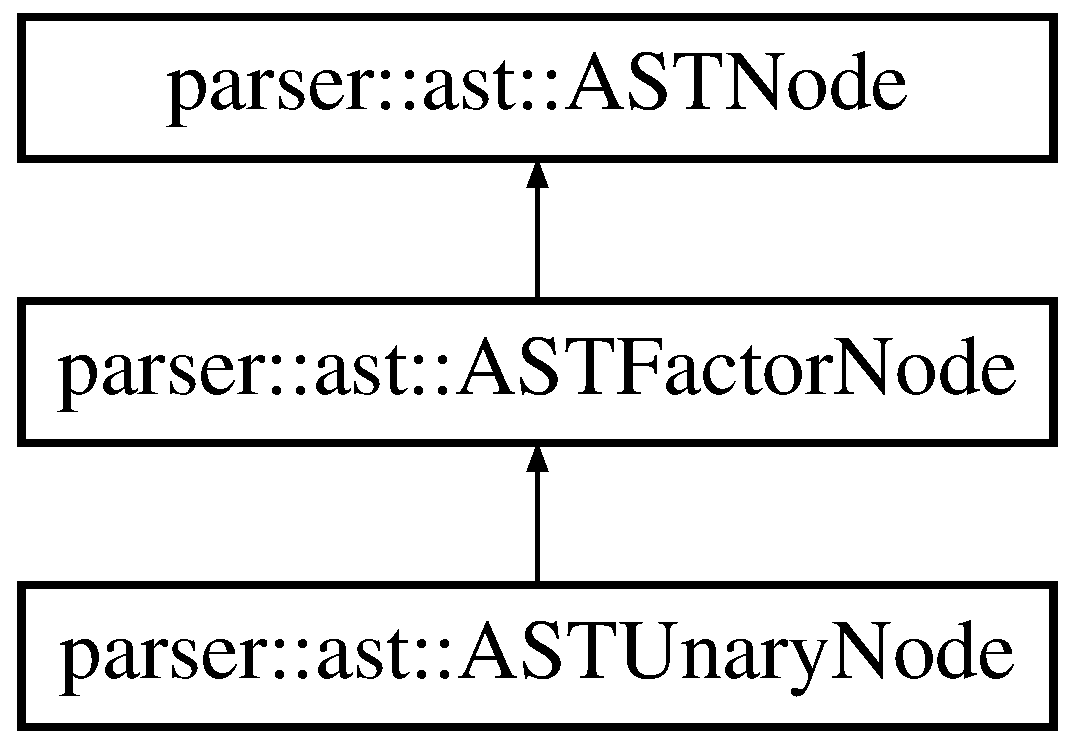
\includegraphics[height=3.000000cm]{d0/d6c/classparser_1_1ast_1_1ASTUnaryNode}
\end{center}
\end{figure}
\subsection*{Public Member Functions}
\begin{DoxyCompactItemize}
\item 
\hyperlink{classparser_1_1ast_1_1ASTUnaryNode_a13654e3c80e4e31f55ad21d6edd6ee29}{A\+S\+T\+Unary\+Node} (\hyperlink{ASTUnaryNode_8h_a3bd5cd6c8af529b35a5e745ad51d5cdf}{Unary\+Operator} \hyperlink{classparser_1_1ast_1_1ASTUnaryNode_a23a33ca1da4fb0fa2756e938e3aea686}{op}, std\+::unique\+\_\+ptr$<$ \hyperlink{classparser_1_1ast_1_1ASTExprNode}{A\+S\+T\+Expr\+Node} $>$ \hyperlink{classparser_1_1ast_1_1ASTUnaryNode_a9c40af1c793969cdefcdbadd953ad0ca}{expr})
\item 
\hyperlink{ASTUnaryNode_8h_a3bd5cd6c8af529b35a5e745ad51d5cdf}{Unary\+Operator} \hyperlink{classparser_1_1ast_1_1ASTUnaryNode_a162e6f618c42d077d526decfde550a48}{get\+Op} () const
\item 
const std\+::unique\+\_\+ptr$<$ \hyperlink{classparser_1_1ast_1_1ASTExprNode}{A\+S\+T\+Expr\+Node} $>$ \& \hyperlink{classparser_1_1ast_1_1ASTUnaryNode_a144541a1fef1be081ad57bfc0ce0039f}{get\+Expr} () const
\item 
const std\+::string \hyperlink{classparser_1_1ast_1_1ASTUnaryNode_ad4c36dae695c49e099bc5deed83ee7da}{get\+Op\+String} () const
\item 
\hyperlink{ASTFactorNode_8h_afbe2fcc03ef15b74a0c1ed1cda7ab0e8}{Factor\+Type} \hyperlink{classparser_1_1ast_1_1ASTUnaryNode_a1056ebc5c34b6f3b0a5485f4cd5ba3c0}{get\+Factor\+Type} () override
\item 
void \hyperlink{classparser_1_1ast_1_1ASTUnaryNode_a4b3bd9c26548e1fb73a82fd5b20add0b}{accept} (\hyperlink{classvisitor_1_1Visitor}{visitor\+::\+Visitor} $\ast$visitor) override
\end{DoxyCompactItemize}
\subsection*{Protected Attributes}
\begin{DoxyCompactItemize}
\item 
\mbox{\Hypertarget{classparser_1_1ast_1_1ASTUnaryNode_a23a33ca1da4fb0fa2756e938e3aea686}\label{classparser_1_1ast_1_1ASTUnaryNode_a23a33ca1da4fb0fa2756e938e3aea686}} 
\hyperlink{ASTUnaryNode_8h_a3bd5cd6c8af529b35a5e745ad51d5cdf}{Unary\+Operator} \hyperlink{classparser_1_1ast_1_1ASTUnaryNode_a23a33ca1da4fb0fa2756e938e3aea686}{op}
\begin{DoxyCompactList}\small\item\em Operator to use for this Unary. \end{DoxyCompactList}\item 
\mbox{\Hypertarget{classparser_1_1ast_1_1ASTUnaryNode_a9c40af1c793969cdefcdbadd953ad0ca}\label{classparser_1_1ast_1_1ASTUnaryNode_a9c40af1c793969cdefcdbadd953ad0ca}} 
std\+::unique\+\_\+ptr$<$ \hyperlink{classparser_1_1ast_1_1ASTExprNode}{A\+S\+T\+Expr\+Node} $>$ \hyperlink{classparser_1_1ast_1_1ASTUnaryNode_a9c40af1c793969cdefcdbadd953ad0ca}{expr}
\begin{DoxyCompactList}\small\item\em Expression for this unary. \end{DoxyCompactList}\end{DoxyCompactItemize}


\subsection{Detailed Description}
Class that represents a unary expression in the A\+ST 

\subsection{Constructor \& Destructor Documentation}
\mbox{\Hypertarget{classparser_1_1ast_1_1ASTUnaryNode_a13654e3c80e4e31f55ad21d6edd6ee29}\label{classparser_1_1ast_1_1ASTUnaryNode_a13654e3c80e4e31f55ad21d6edd6ee29}} 
\index{parser\+::ast\+::\+A\+S\+T\+Unary\+Node@{parser\+::ast\+::\+A\+S\+T\+Unary\+Node}!A\+S\+T\+Unary\+Node@{A\+S\+T\+Unary\+Node}}
\index{A\+S\+T\+Unary\+Node@{A\+S\+T\+Unary\+Node}!parser\+::ast\+::\+A\+S\+T\+Unary\+Node@{parser\+::ast\+::\+A\+S\+T\+Unary\+Node}}
\subsubsection{\texorpdfstring{A\+S\+T\+Unary\+Node()}{ASTUnaryNode()}}
{\footnotesize\ttfamily parser\+::ast\+::\+A\+S\+T\+Unary\+Node\+::\+A\+S\+T\+Unary\+Node (\begin{DoxyParamCaption}\item[{\hyperlink{ASTUnaryNode_8h_a3bd5cd6c8af529b35a5e745ad51d5cdf}{Unary\+Operator}}]{op,  }\item[{std\+::unique\+\_\+ptr$<$ \hyperlink{classparser_1_1ast_1_1ASTExprNode}{A\+S\+T\+Expr\+Node} $>$}]{expr }\end{DoxyParamCaption})}

Constructor to use for this class 
\begin{DoxyParams}{Parameters}
{\em op} & The operator \\
\hline
{\em expr} & The expression it is applied on \\
\hline
\end{DoxyParams}


\subsection{Member Function Documentation}
\mbox{\Hypertarget{classparser_1_1ast_1_1ASTUnaryNode_a4b3bd9c26548e1fb73a82fd5b20add0b}\label{classparser_1_1ast_1_1ASTUnaryNode_a4b3bd9c26548e1fb73a82fd5b20add0b}} 
\index{parser\+::ast\+::\+A\+S\+T\+Unary\+Node@{parser\+::ast\+::\+A\+S\+T\+Unary\+Node}!accept@{accept}}
\index{accept@{accept}!parser\+::ast\+::\+A\+S\+T\+Unary\+Node@{parser\+::ast\+::\+A\+S\+T\+Unary\+Node}}
\subsubsection{\texorpdfstring{accept()}{accept()}}
{\footnotesize\ttfamily void parser\+::ast\+::\+A\+S\+T\+Unary\+Node\+::accept (\begin{DoxyParamCaption}\item[{\hyperlink{classvisitor_1_1Visitor}{visitor\+::\+Visitor} $\ast$}]{visitor }\end{DoxyParamCaption})\hspace{0.3cm}{\ttfamily [override]}, {\ttfamily [virtual]}}

Accepts a visitor and calls the operation by invoking {\ttfamily visit(this)} 
\begin{DoxyParams}{Parameters}
{\em visitor} & the visitor to accept \\
\hline
\end{DoxyParams}


Implements \hyperlink{classparser_1_1ast_1_1ASTNode_a3ff84fdfdbbc5c39b70b4d04c22e7dc3}{parser\+::ast\+::\+A\+S\+T\+Node}.

\mbox{\Hypertarget{classparser_1_1ast_1_1ASTUnaryNode_a144541a1fef1be081ad57bfc0ce0039f}\label{classparser_1_1ast_1_1ASTUnaryNode_a144541a1fef1be081ad57bfc0ce0039f}} 
\index{parser\+::ast\+::\+A\+S\+T\+Unary\+Node@{parser\+::ast\+::\+A\+S\+T\+Unary\+Node}!get\+Expr@{get\+Expr}}
\index{get\+Expr@{get\+Expr}!parser\+::ast\+::\+A\+S\+T\+Unary\+Node@{parser\+::ast\+::\+A\+S\+T\+Unary\+Node}}
\subsubsection{\texorpdfstring{get\+Expr()}{getExpr()}}
{\footnotesize\ttfamily const std\+::unique\+\_\+ptr$<$ \hyperlink{classparser_1_1ast_1_1ASTExprNode}{parser\+::ast\+::\+A\+S\+T\+Expr\+Node} $>$ \& parser\+::ast\+::\+A\+S\+T\+Unary\+Node\+::get\+Expr (\begin{DoxyParamCaption}{ }\end{DoxyParamCaption}) const}

\begin{DoxyReturn}{Returns}
the expression after the operator 
\end{DoxyReturn}
\mbox{\Hypertarget{classparser_1_1ast_1_1ASTUnaryNode_a1056ebc5c34b6f3b0a5485f4cd5ba3c0}\label{classparser_1_1ast_1_1ASTUnaryNode_a1056ebc5c34b6f3b0a5485f4cd5ba3c0}} 
\index{parser\+::ast\+::\+A\+S\+T\+Unary\+Node@{parser\+::ast\+::\+A\+S\+T\+Unary\+Node}!get\+Factor\+Type@{get\+Factor\+Type}}
\index{get\+Factor\+Type@{get\+Factor\+Type}!parser\+::ast\+::\+A\+S\+T\+Unary\+Node@{parser\+::ast\+::\+A\+S\+T\+Unary\+Node}}
\subsubsection{\texorpdfstring{get\+Factor\+Type()}{getFactorType()}}
{\footnotesize\ttfamily \hyperlink{ASTFactorNode_8h_afbe2fcc03ef15b74a0c1ed1cda7ab0e8}{parser\+::ast\+::\+Factor\+Type} parser\+::ast\+::\+A\+S\+T\+Unary\+Node\+::get\+Factor\+Type (\begin{DoxyParamCaption}{ }\end{DoxyParamCaption})\hspace{0.3cm}{\ttfamily [override]}, {\ttfamily [virtual]}}

\begin{DoxyReturn}{Returns}
The type of factor this is. Use instead of checking the class type. 
\end{DoxyReturn}


Implements \hyperlink{classparser_1_1ast_1_1ASTFactorNode_a13eea7f949c0055dea0a9d7b715f16a8}{parser\+::ast\+::\+A\+S\+T\+Factor\+Node}.

\mbox{\Hypertarget{classparser_1_1ast_1_1ASTUnaryNode_a162e6f618c42d077d526decfde550a48}\label{classparser_1_1ast_1_1ASTUnaryNode_a162e6f618c42d077d526decfde550a48}} 
\index{parser\+::ast\+::\+A\+S\+T\+Unary\+Node@{parser\+::ast\+::\+A\+S\+T\+Unary\+Node}!get\+Op@{get\+Op}}
\index{get\+Op@{get\+Op}!parser\+::ast\+::\+A\+S\+T\+Unary\+Node@{parser\+::ast\+::\+A\+S\+T\+Unary\+Node}}
\subsubsection{\texorpdfstring{get\+Op()}{getOp()}}
{\footnotesize\ttfamily \hyperlink{ASTUnaryNode_8h_a3bd5cd6c8af529b35a5e745ad51d5cdf}{parser\+::ast\+::\+Unary\+Operator} parser\+::ast\+::\+A\+S\+T\+Unary\+Node\+::get\+Op (\begin{DoxyParamCaption}{ }\end{DoxyParamCaption}) const}

\begin{DoxyReturn}{Returns}
the unary operator 
\end{DoxyReturn}
\mbox{\Hypertarget{classparser_1_1ast_1_1ASTUnaryNode_ad4c36dae695c49e099bc5deed83ee7da}\label{classparser_1_1ast_1_1ASTUnaryNode_ad4c36dae695c49e099bc5deed83ee7da}} 
\index{parser\+::ast\+::\+A\+S\+T\+Unary\+Node@{parser\+::ast\+::\+A\+S\+T\+Unary\+Node}!get\+Op\+String@{get\+Op\+String}}
\index{get\+Op\+String@{get\+Op\+String}!parser\+::ast\+::\+A\+S\+T\+Unary\+Node@{parser\+::ast\+::\+A\+S\+T\+Unary\+Node}}
\subsubsection{\texorpdfstring{get\+Op\+String()}{getOpString()}}
{\footnotesize\ttfamily const std\+::string parser\+::ast\+::\+A\+S\+T\+Unary\+Node\+::get\+Op\+String (\begin{DoxyParamCaption}{ }\end{DoxyParamCaption}) const}

Converts a Unary Operator to a string representation of it 
\begin{DoxyParams}{Parameters}
{\em op} & the operator to convert to a string \\
\hline
\end{DoxyParams}
\begin{DoxyReturn}{Returns}
the string representation of that operator 
\end{DoxyReturn}


The documentation for this class was generated from the following files\+:\begin{DoxyCompactItemize}
\item 
parser/ast/expression/factor/\hyperlink{ASTUnaryNode_8h}{A\+S\+T\+Unary\+Node.\+h}\item 
parser/ast/expression/factor/\hyperlink{ASTUnaryNode_8cpp}{A\+S\+T\+Unary\+Node.\+cpp}\end{DoxyCompactItemize}

\hypertarget{classparser_1_1ast_1_1ASTVariableDeclStatementNode}{}\section{parser\+:\+:ast\+:\+:A\+S\+T\+Variable\+Decl\+Statement\+Node Class Reference}
\label{classparser_1_1ast_1_1ASTVariableDeclStatementNode}\index{parser\+::ast\+::\+A\+S\+T\+Variable\+Decl\+Statement\+Node@{parser\+::ast\+::\+A\+S\+T\+Variable\+Decl\+Statement\+Node}}


{\ttfamily \#include $<$A\+S\+T\+Variable\+Decl\+Statement\+Node.\+h$>$}

Inheritance diagram for parser\+:\+:ast\+:\+:A\+S\+T\+Variable\+Decl\+Statement\+Node\+:\begin{figure}[H]
\begin{center}
\leavevmode
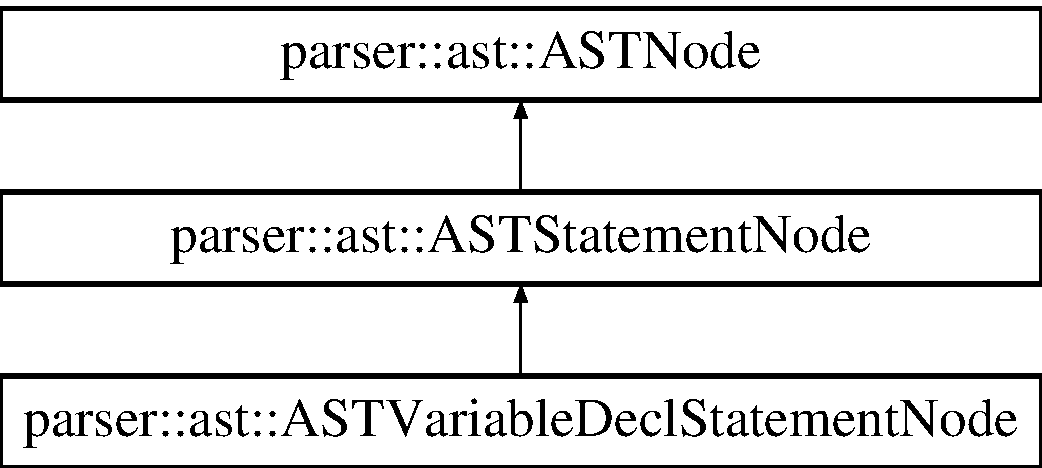
\includegraphics[height=3.000000cm]{d6/d12/classparser_1_1ast_1_1ASTVariableDeclStatementNode}
\end{center}
\end{figure}
\subsection*{Public Member Functions}
\begin{DoxyCompactItemize}
\item 
\hyperlink{classparser_1_1ast_1_1ASTVariableDeclStatementNode_ab05aabaf5dd61a54a3b05101c9457260}{A\+S\+T\+Variable\+Decl\+Statement\+Node} (std\+::unique\+\_\+ptr$<$ \hyperlink{classparser_1_1ast_1_1ASTIdentifierNode}{A\+S\+T\+Identifier\+Node} $>$ \hyperlink{classparser_1_1ast_1_1ASTVariableDeclStatementNode_ac835afc9e99d1e9e1af10db2ade9f901}{identifier}, \hyperlink{ASTVariableDeclStatementNode_8h_a1e8e1bde0729627e3a22ffa858d5f3b9}{Variable\+Type} \hyperlink{classparser_1_1ast_1_1ASTVariableDeclStatementNode_a03d5695c58afabacdbfcf98950a65493}{type}, std\+::unique\+\_\+ptr$<$ \hyperlink{classparser_1_1ast_1_1ASTExprNode}{A\+S\+T\+Expr\+Node} $>$ \hyperlink{classparser_1_1ast_1_1ASTVariableDeclStatementNode_a5c648465737a76a89f91750b56741557}{expr})
\item 
std\+::unique\+\_\+ptr$<$ \hyperlink{classparser_1_1ast_1_1ASTIdentifierNode}{A\+S\+T\+Identifier\+Node} $>$ \& \hyperlink{classparser_1_1ast_1_1ASTVariableDeclStatementNode_add29f076ef275098eb63064e2441d4dd}{get\+Identifier} ()
\item 
\hyperlink{ASTVariableDeclStatementNode_8h_a1e8e1bde0729627e3a22ffa858d5f3b9}{Variable\+Type} \hyperlink{classparser_1_1ast_1_1ASTVariableDeclStatementNode_a5f26584b63fff33a9bc55c595ab1d3ab}{get\+Type} () const
\item 
std\+::unique\+\_\+ptr$<$ \hyperlink{classparser_1_1ast_1_1ASTExprNode}{A\+S\+T\+Expr\+Node} $>$ \& \hyperlink{classparser_1_1ast_1_1ASTVariableDeclStatementNode_aaa330017ed4652ecb8d9900ac774b60f}{get\+Expr} ()
\item 
Statement\+Type \hyperlink{classparser_1_1ast_1_1ASTVariableDeclStatementNode_a273b2c22a426022608813603ddfd820b}{get\+Statement\+Type} () override
\item 
void \hyperlink{classparser_1_1ast_1_1ASTVariableDeclStatementNode_a4448c73408ed86719c6f3993a4eb8869}{accept} (\hyperlink{classvisitor_1_1Visitor}{visitor\+::\+Visitor} $\ast$visitor) override
\end{DoxyCompactItemize}
\subsection*{Protected Attributes}
\begin{DoxyCompactItemize}
\item 
\mbox{\Hypertarget{classparser_1_1ast_1_1ASTVariableDeclStatementNode_ac835afc9e99d1e9e1af10db2ade9f901}\label{classparser_1_1ast_1_1ASTVariableDeclStatementNode_ac835afc9e99d1e9e1af10db2ade9f901}} 
std\+::unique\+\_\+ptr$<$ \hyperlink{classparser_1_1ast_1_1ASTIdentifierNode}{A\+S\+T\+Identifier\+Node} $>$ \hyperlink{classparser_1_1ast_1_1ASTVariableDeclStatementNode_ac835afc9e99d1e9e1af10db2ade9f901}{identifier}
\begin{DoxyCompactList}\small\item\em The variable identifier. \end{DoxyCompactList}\item 
\mbox{\Hypertarget{classparser_1_1ast_1_1ASTVariableDeclStatementNode_a03d5695c58afabacdbfcf98950a65493}\label{classparser_1_1ast_1_1ASTVariableDeclStatementNode_a03d5695c58afabacdbfcf98950a65493}} 
\hyperlink{ASTVariableDeclStatementNode_8h_a1e8e1bde0729627e3a22ffa858d5f3b9}{Variable\+Type} \hyperlink{classparser_1_1ast_1_1ASTVariableDeclStatementNode_a03d5695c58afabacdbfcf98950a65493}{type}
\begin{DoxyCompactList}\small\item\em The variable type. \end{DoxyCompactList}\item 
\mbox{\Hypertarget{classparser_1_1ast_1_1ASTVariableDeclStatementNode_a5c648465737a76a89f91750b56741557}\label{classparser_1_1ast_1_1ASTVariableDeclStatementNode_a5c648465737a76a89f91750b56741557}} 
std\+::unique\+\_\+ptr$<$ \hyperlink{classparser_1_1ast_1_1ASTExprNode}{A\+S\+T\+Expr\+Node} $>$ \hyperlink{classparser_1_1ast_1_1ASTVariableDeclStatementNode_a5c648465737a76a89f91750b56741557}{expr}
\begin{DoxyCompactList}\small\item\em The expression making up this variable. \end{DoxyCompactList}\end{DoxyCompactItemize}


\subsection{Detailed Description}
The \hyperlink{classparser_1_1ast_1_1ASTVariableDeclStatementNode}{A\+S\+T\+Variable\+Decl\+Statement\+Node} represents an A\+ST node for a Variable Decleration Sentential form in the Mini\+Lang Language 

\subsection{Constructor \& Destructor Documentation}
\mbox{\Hypertarget{classparser_1_1ast_1_1ASTVariableDeclStatementNode_ab05aabaf5dd61a54a3b05101c9457260}\label{classparser_1_1ast_1_1ASTVariableDeclStatementNode_ab05aabaf5dd61a54a3b05101c9457260}} 
\index{parser\+::ast\+::\+A\+S\+T\+Variable\+Decl\+Statement\+Node@{parser\+::ast\+::\+A\+S\+T\+Variable\+Decl\+Statement\+Node}!A\+S\+T\+Variable\+Decl\+Statement\+Node@{A\+S\+T\+Variable\+Decl\+Statement\+Node}}
\index{A\+S\+T\+Variable\+Decl\+Statement\+Node@{A\+S\+T\+Variable\+Decl\+Statement\+Node}!parser\+::ast\+::\+A\+S\+T\+Variable\+Decl\+Statement\+Node@{parser\+::ast\+::\+A\+S\+T\+Variable\+Decl\+Statement\+Node}}
\subsubsection{\texorpdfstring{A\+S\+T\+Variable\+Decl\+Statement\+Node()}{ASTVariableDeclStatementNode()}}
{\footnotesize\ttfamily parser\+::ast\+::\+A\+S\+T\+Variable\+Decl\+Statement\+Node\+::\+A\+S\+T\+Variable\+Decl\+Statement\+Node (\begin{DoxyParamCaption}\item[{std\+::unique\+\_\+ptr$<$ \hyperlink{classparser_1_1ast_1_1ASTIdentifierNode}{A\+S\+T\+Identifier\+Node} $>$}]{identifier,  }\item[{\hyperlink{ASTVariableDeclStatementNode_8h_a1e8e1bde0729627e3a22ffa858d5f3b9}{Variable\+Type}}]{type,  }\item[{std\+::unique\+\_\+ptr$<$ \hyperlink{classparser_1_1ast_1_1ASTExprNode}{A\+S\+T\+Expr\+Node} $>$}]{expr }\end{DoxyParamCaption})}

Consturctor when the expression node is already created. 
\begin{DoxyParams}{Parameters}
{\em identifier} & the variable identifier \\
\hline
{\em type} & the variable type, can be one of
\begin{DoxyItemize}
\item {\ttfamily Variable\+Type\+::\+V\+A\+R\+\_\+\+I\+NT}
\item {\ttfamily Variable\+Type\+::\+V\+A\+R\+\_\+\+R\+E\+AL}
\item {\ttfamily Variable\+Type\+::\+V\+A\+R\+\_\+\+B\+O\+OL}
\item {\ttfamily Variable\+Type\+::\+V\+A\+R\+\_\+\+S\+T\+R\+I\+NG} 
\end{DoxyItemize}\\
\hline
{\em exp} & The Expression node that will make up this variable. \\
\hline
\end{DoxyParams}


\subsection{Member Function Documentation}
\mbox{\Hypertarget{classparser_1_1ast_1_1ASTVariableDeclStatementNode_a4448c73408ed86719c6f3993a4eb8869}\label{classparser_1_1ast_1_1ASTVariableDeclStatementNode_a4448c73408ed86719c6f3993a4eb8869}} 
\index{parser\+::ast\+::\+A\+S\+T\+Variable\+Decl\+Statement\+Node@{parser\+::ast\+::\+A\+S\+T\+Variable\+Decl\+Statement\+Node}!accept@{accept}}
\index{accept@{accept}!parser\+::ast\+::\+A\+S\+T\+Variable\+Decl\+Statement\+Node@{parser\+::ast\+::\+A\+S\+T\+Variable\+Decl\+Statement\+Node}}
\subsubsection{\texorpdfstring{accept()}{accept()}}
{\footnotesize\ttfamily void parser\+::ast\+::\+A\+S\+T\+Variable\+Decl\+Statement\+Node\+::accept (\begin{DoxyParamCaption}\item[{\hyperlink{classvisitor_1_1Visitor}{visitor\+::\+Visitor} $\ast$}]{visitor }\end{DoxyParamCaption})\hspace{0.3cm}{\ttfamily [override]}, {\ttfamily [virtual]}}

Accepts a visitor and calls the operation by invoking {\ttfamily visit(this)} 
\begin{DoxyParams}{Parameters}
{\em visitor} & the visitor to accept \\
\hline
\end{DoxyParams}


Implements \hyperlink{classparser_1_1ast_1_1ASTNode_a3ff84fdfdbbc5c39b70b4d04c22e7dc3}{parser\+::ast\+::\+A\+S\+T\+Node}.

\mbox{\Hypertarget{classparser_1_1ast_1_1ASTVariableDeclStatementNode_aaa330017ed4652ecb8d9900ac774b60f}\label{classparser_1_1ast_1_1ASTVariableDeclStatementNode_aaa330017ed4652ecb8d9900ac774b60f}} 
\index{parser\+::ast\+::\+A\+S\+T\+Variable\+Decl\+Statement\+Node@{parser\+::ast\+::\+A\+S\+T\+Variable\+Decl\+Statement\+Node}!get\+Expr@{get\+Expr}}
\index{get\+Expr@{get\+Expr}!parser\+::ast\+::\+A\+S\+T\+Variable\+Decl\+Statement\+Node@{parser\+::ast\+::\+A\+S\+T\+Variable\+Decl\+Statement\+Node}}
\subsubsection{\texorpdfstring{get\+Expr()}{getExpr()}}
{\footnotesize\ttfamily std\+::unique\+\_\+ptr$<$ \hyperlink{classparser_1_1ast_1_1ASTExprNode}{parser\+::ast\+::\+A\+S\+T\+Expr\+Node} $>$ \& parser\+::ast\+::\+A\+S\+T\+Variable\+Decl\+Statement\+Node\+::get\+Expr (\begin{DoxyParamCaption}{ }\end{DoxyParamCaption})}

\begin{DoxyReturn}{Returns}
The expression node to create this variable 
\end{DoxyReturn}
\mbox{\Hypertarget{classparser_1_1ast_1_1ASTVariableDeclStatementNode_add29f076ef275098eb63064e2441d4dd}\label{classparser_1_1ast_1_1ASTVariableDeclStatementNode_add29f076ef275098eb63064e2441d4dd}} 
\index{parser\+::ast\+::\+A\+S\+T\+Variable\+Decl\+Statement\+Node@{parser\+::ast\+::\+A\+S\+T\+Variable\+Decl\+Statement\+Node}!get\+Identifier@{get\+Identifier}}
\index{get\+Identifier@{get\+Identifier}!parser\+::ast\+::\+A\+S\+T\+Variable\+Decl\+Statement\+Node@{parser\+::ast\+::\+A\+S\+T\+Variable\+Decl\+Statement\+Node}}
\subsubsection{\texorpdfstring{get\+Identifier()}{getIdentifier()}}
{\footnotesize\ttfamily std\+::unique\+\_\+ptr$<$ \hyperlink{classparser_1_1ast_1_1ASTIdentifierNode}{parser\+::ast\+::\+A\+S\+T\+Identifier\+Node} $>$ \& parser\+::ast\+::\+A\+S\+T\+Variable\+Decl\+Statement\+Node\+::get\+Identifier (\begin{DoxyParamCaption}{ }\end{DoxyParamCaption})}

\begin{DoxyReturn}{Returns}
The variable identifier 
\end{DoxyReturn}
\mbox{\Hypertarget{classparser_1_1ast_1_1ASTVariableDeclStatementNode_a273b2c22a426022608813603ddfd820b}\label{classparser_1_1ast_1_1ASTVariableDeclStatementNode_a273b2c22a426022608813603ddfd820b}} 
\index{parser\+::ast\+::\+A\+S\+T\+Variable\+Decl\+Statement\+Node@{parser\+::ast\+::\+A\+S\+T\+Variable\+Decl\+Statement\+Node}!get\+Statement\+Type@{get\+Statement\+Type}}
\index{get\+Statement\+Type@{get\+Statement\+Type}!parser\+::ast\+::\+A\+S\+T\+Variable\+Decl\+Statement\+Node@{parser\+::ast\+::\+A\+S\+T\+Variable\+Decl\+Statement\+Node}}
\subsubsection{\texorpdfstring{get\+Statement\+Type()}{getStatementType()}}
{\footnotesize\ttfamily parser\+::ast\+::\+Statement\+Type parser\+::ast\+::\+A\+S\+T\+Variable\+Decl\+Statement\+Node\+::get\+Statement\+Type (\begin{DoxyParamCaption}{ }\end{DoxyParamCaption})\hspace{0.3cm}{\ttfamily [override]}, {\ttfamily [virtual]}}

Virtual Method to return the statement type \begin{DoxyReturn}{Returns}
The statement type (instead of checking what class it\textquotesingle{}s an instance of) 
\end{DoxyReturn}


Implements \hyperlink{classparser_1_1ast_1_1ASTStatementNode_ac381d35d12f774a1bab0e209c5bfec1f}{parser\+::ast\+::\+A\+S\+T\+Statement\+Node}.

\mbox{\Hypertarget{classparser_1_1ast_1_1ASTVariableDeclStatementNode_a5f26584b63fff33a9bc55c595ab1d3ab}\label{classparser_1_1ast_1_1ASTVariableDeclStatementNode_a5f26584b63fff33a9bc55c595ab1d3ab}} 
\index{parser\+::ast\+::\+A\+S\+T\+Variable\+Decl\+Statement\+Node@{parser\+::ast\+::\+A\+S\+T\+Variable\+Decl\+Statement\+Node}!get\+Type@{get\+Type}}
\index{get\+Type@{get\+Type}!parser\+::ast\+::\+A\+S\+T\+Variable\+Decl\+Statement\+Node@{parser\+::ast\+::\+A\+S\+T\+Variable\+Decl\+Statement\+Node}}
\subsubsection{\texorpdfstring{get\+Type()}{getType()}}
{\footnotesize\ttfamily \hyperlink{ASTVariableDeclStatementNode_8h_a1e8e1bde0729627e3a22ffa858d5f3b9}{parser\+::ast\+::\+Variable\+Type} parser\+::ast\+::\+A\+S\+T\+Variable\+Decl\+Statement\+Node\+::get\+Type (\begin{DoxyParamCaption}{ }\end{DoxyParamCaption}) const}

\begin{DoxyReturn}{Returns}
The variable type 
\end{DoxyReturn}


The documentation for this class was generated from the following files\+:\begin{DoxyCompactItemize}
\item 
parser/ast/statement/\hyperlink{ASTVariableDeclStatementNode_8h}{A\+S\+T\+Variable\+Decl\+Statement\+Node.\+h}\item 
parser/ast/statement/A\+S\+T\+Variable\+Decl\+Statement\+Node.\+cpp\end{DoxyCompactItemize}

\hypertarget{classparser_1_1ast_1_1ASTWhileStatementNode}{}\section{parser\+:\+:ast\+:\+:A\+S\+T\+While\+Statement\+Node Class Reference}
\label{classparser_1_1ast_1_1ASTWhileStatementNode}\index{parser\+::ast\+::\+A\+S\+T\+While\+Statement\+Node@{parser\+::ast\+::\+A\+S\+T\+While\+Statement\+Node}}


{\ttfamily \#include $<$A\+S\+T\+While\+Statement\+Node.\+h$>$}

Inheritance diagram for parser\+:\+:ast\+:\+:A\+S\+T\+While\+Statement\+Node\+:\begin{figure}[H]
\begin{center}
\leavevmode
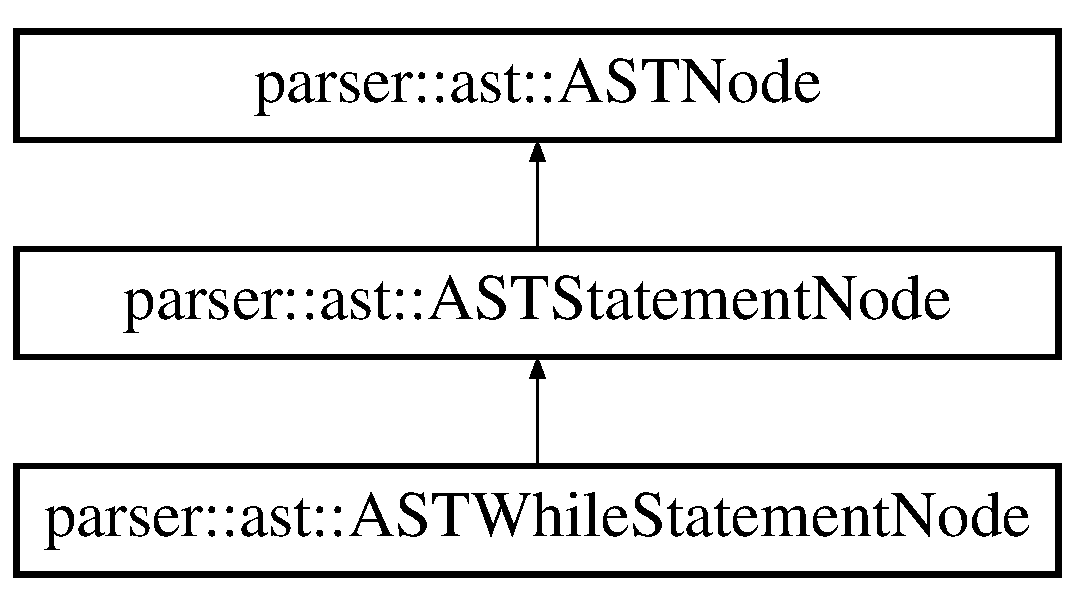
\includegraphics[height=3.000000cm]{dd/d51/classparser_1_1ast_1_1ASTWhileStatementNode}
\end{center}
\end{figure}
\subsection*{Public Member Functions}
\begin{DoxyCompactItemize}
\item 
\hyperlink{classparser_1_1ast_1_1ASTWhileStatementNode_a099a29ffe3bca12fac6a7904d52b9c6a}{A\+S\+T\+While\+Statement\+Node} (std\+::unique\+\_\+ptr$<$ \hyperlink{classparser_1_1ast_1_1ASTExprNode}{A\+S\+T\+Expr\+Node} $>$ \hyperlink{classparser_1_1ast_1_1ASTWhileStatementNode_aef13a0ab19cfd381066af8c066e341e1}{predicate}, std\+::unique\+\_\+ptr$<$ \hyperlink{classparser_1_1ast_1_1ASTBlockStatementNode}{A\+S\+T\+Block\+Statement\+Node} $>$ \hyperlink{classparser_1_1ast_1_1ASTWhileStatementNode_ae88c633373308600c37d89db84980363}{loop\+Block})
\item 
std\+::unique\+\_\+ptr$<$ \hyperlink{classparser_1_1ast_1_1ASTExprNode}{A\+S\+T\+Expr\+Node} $>$ \& \hyperlink{classparser_1_1ast_1_1ASTWhileStatementNode_af0a556a314a4b06858d8f47c94e64b86}{get\+Predicate} ()
\item 
std\+::unique\+\_\+ptr$<$ \hyperlink{classparser_1_1ast_1_1ASTBlockStatementNode}{A\+S\+T\+Block\+Statement\+Node} $>$ \& \hyperlink{classparser_1_1ast_1_1ASTWhileStatementNode_a17d4d7573477af83900a6dda33c29e78}{get\+Loop\+Block} ()
\item 
Statement\+Type \hyperlink{classparser_1_1ast_1_1ASTWhileStatementNode_a47ad4212e8bae1bbe602918044e39cd8}{get\+Statement\+Type} () override
\item 
void \hyperlink{classparser_1_1ast_1_1ASTWhileStatementNode_a448a46d9dbde688562ada266192735c8}{accept} (\hyperlink{classvisitor_1_1Visitor}{visitor\+::\+Visitor} $\ast$visitor) override
\end{DoxyCompactItemize}
\subsection*{Protected Attributes}
\begin{DoxyCompactItemize}
\item 
\mbox{\Hypertarget{classparser_1_1ast_1_1ASTWhileStatementNode_aef13a0ab19cfd381066af8c066e341e1}\label{classparser_1_1ast_1_1ASTWhileStatementNode_aef13a0ab19cfd381066af8c066e341e1}} 
std\+::unique\+\_\+ptr$<$ \hyperlink{classparser_1_1ast_1_1ASTExprNode}{A\+S\+T\+Expr\+Node} $>$ \hyperlink{classparser_1_1ast_1_1ASTWhileStatementNode_aef13a0ab19cfd381066af8c066e341e1}{predicate}
\begin{DoxyCompactList}\small\item\em The predicate to be satisfied for the loop to keep executing. \end{DoxyCompactList}\item 
\mbox{\Hypertarget{classparser_1_1ast_1_1ASTWhileStatementNode_ae88c633373308600c37d89db84980363}\label{classparser_1_1ast_1_1ASTWhileStatementNode_ae88c633373308600c37d89db84980363}} 
std\+::unique\+\_\+ptr$<$ \hyperlink{classparser_1_1ast_1_1ASTBlockStatementNode}{A\+S\+T\+Block\+Statement\+Node} $>$ \hyperlink{classparser_1_1ast_1_1ASTWhileStatementNode_ae88c633373308600c37d89db84980363}{loop\+Block}
\begin{DoxyCompactList}\small\item\em The block to be executed in the while loop. \end{DoxyCompactList}\end{DoxyCompactItemize}


\subsection{Detailed Description}
This class represents a while statement node in the A\+ST for the Minilang language 

\subsection{Constructor \& Destructor Documentation}
\mbox{\Hypertarget{classparser_1_1ast_1_1ASTWhileStatementNode_a099a29ffe3bca12fac6a7904d52b9c6a}\label{classparser_1_1ast_1_1ASTWhileStatementNode_a099a29ffe3bca12fac6a7904d52b9c6a}} 
\index{parser\+::ast\+::\+A\+S\+T\+While\+Statement\+Node@{parser\+::ast\+::\+A\+S\+T\+While\+Statement\+Node}!A\+S\+T\+While\+Statement\+Node@{A\+S\+T\+While\+Statement\+Node}}
\index{A\+S\+T\+While\+Statement\+Node@{A\+S\+T\+While\+Statement\+Node}!parser\+::ast\+::\+A\+S\+T\+While\+Statement\+Node@{parser\+::ast\+::\+A\+S\+T\+While\+Statement\+Node}}
\subsubsection{\texorpdfstring{A\+S\+T\+While\+Statement\+Node()}{ASTWhileStatementNode()}}
{\footnotesize\ttfamily parser\+::ast\+::\+A\+S\+T\+While\+Statement\+Node\+::\+A\+S\+T\+While\+Statement\+Node (\begin{DoxyParamCaption}\item[{std\+::unique\+\_\+ptr$<$ \hyperlink{classparser_1_1ast_1_1ASTExprNode}{A\+S\+T\+Expr\+Node} $>$}]{predicate,  }\item[{std\+::unique\+\_\+ptr$<$ \hyperlink{classparser_1_1ast_1_1ASTBlockStatementNode}{A\+S\+T\+Block\+Statement\+Node} $>$}]{loop\+Block }\end{DoxyParamCaption})}

The constructor for this object 
\begin{DoxyParams}{Parameters}
{\em predicate} & The predicate that needs to be satsified to keep looping \\
\hline
{\em loop\+Block} & The block to be executed in the while loop (while the predicate holds) \\
\hline
\end{DoxyParams}


\subsection{Member Function Documentation}
\mbox{\Hypertarget{classparser_1_1ast_1_1ASTWhileStatementNode_a448a46d9dbde688562ada266192735c8}\label{classparser_1_1ast_1_1ASTWhileStatementNode_a448a46d9dbde688562ada266192735c8}} 
\index{parser\+::ast\+::\+A\+S\+T\+While\+Statement\+Node@{parser\+::ast\+::\+A\+S\+T\+While\+Statement\+Node}!accept@{accept}}
\index{accept@{accept}!parser\+::ast\+::\+A\+S\+T\+While\+Statement\+Node@{parser\+::ast\+::\+A\+S\+T\+While\+Statement\+Node}}
\subsubsection{\texorpdfstring{accept()}{accept()}}
{\footnotesize\ttfamily void parser\+::ast\+::\+A\+S\+T\+While\+Statement\+Node\+::accept (\begin{DoxyParamCaption}\item[{\hyperlink{classvisitor_1_1Visitor}{visitor\+::\+Visitor} $\ast$}]{visitor }\end{DoxyParamCaption})\hspace{0.3cm}{\ttfamily [override]}, {\ttfamily [virtual]}}

Accepts a visitor and calls the operation by invoking {\ttfamily visit(this)} 
\begin{DoxyParams}{Parameters}
{\em visitor} & the visitor to accept \\
\hline
\end{DoxyParams}


Implements \hyperlink{classparser_1_1ast_1_1ASTNode_a3ff84fdfdbbc5c39b70b4d04c22e7dc3}{parser\+::ast\+::\+A\+S\+T\+Node}.

\mbox{\Hypertarget{classparser_1_1ast_1_1ASTWhileStatementNode_a17d4d7573477af83900a6dda33c29e78}\label{classparser_1_1ast_1_1ASTWhileStatementNode_a17d4d7573477af83900a6dda33c29e78}} 
\index{parser\+::ast\+::\+A\+S\+T\+While\+Statement\+Node@{parser\+::ast\+::\+A\+S\+T\+While\+Statement\+Node}!get\+Loop\+Block@{get\+Loop\+Block}}
\index{get\+Loop\+Block@{get\+Loop\+Block}!parser\+::ast\+::\+A\+S\+T\+While\+Statement\+Node@{parser\+::ast\+::\+A\+S\+T\+While\+Statement\+Node}}
\subsubsection{\texorpdfstring{get\+Loop\+Block()}{getLoopBlock()}}
{\footnotesize\ttfamily std\+::unique\+\_\+ptr$<$ \hyperlink{classparser_1_1ast_1_1ASTBlockStatementNode}{parser\+::ast\+::\+A\+S\+T\+Block\+Statement\+Node} $>$ \& parser\+::ast\+::\+A\+S\+T\+While\+Statement\+Node\+::get\+Loop\+Block (\begin{DoxyParamCaption}{ }\end{DoxyParamCaption})}

\begin{DoxyReturn}{Returns}
the block to be executed in the while loop (while the predicate holds) 
\end{DoxyReturn}
\mbox{\Hypertarget{classparser_1_1ast_1_1ASTWhileStatementNode_af0a556a314a4b06858d8f47c94e64b86}\label{classparser_1_1ast_1_1ASTWhileStatementNode_af0a556a314a4b06858d8f47c94e64b86}} 
\index{parser\+::ast\+::\+A\+S\+T\+While\+Statement\+Node@{parser\+::ast\+::\+A\+S\+T\+While\+Statement\+Node}!get\+Predicate@{get\+Predicate}}
\index{get\+Predicate@{get\+Predicate}!parser\+::ast\+::\+A\+S\+T\+While\+Statement\+Node@{parser\+::ast\+::\+A\+S\+T\+While\+Statement\+Node}}
\subsubsection{\texorpdfstring{get\+Predicate()}{getPredicate()}}
{\footnotesize\ttfamily std\+::unique\+\_\+ptr$<$ \hyperlink{classparser_1_1ast_1_1ASTExprNode}{parser\+::ast\+::\+A\+S\+T\+Expr\+Node} $>$ \& parser\+::ast\+::\+A\+S\+T\+While\+Statement\+Node\+::get\+Predicate (\begin{DoxyParamCaption}{ }\end{DoxyParamCaption})}

\begin{DoxyReturn}{Returns}
the predicate that needs to be satsified to keep looping 
\end{DoxyReturn}
\mbox{\Hypertarget{classparser_1_1ast_1_1ASTWhileStatementNode_a47ad4212e8bae1bbe602918044e39cd8}\label{classparser_1_1ast_1_1ASTWhileStatementNode_a47ad4212e8bae1bbe602918044e39cd8}} 
\index{parser\+::ast\+::\+A\+S\+T\+While\+Statement\+Node@{parser\+::ast\+::\+A\+S\+T\+While\+Statement\+Node}!get\+Statement\+Type@{get\+Statement\+Type}}
\index{get\+Statement\+Type@{get\+Statement\+Type}!parser\+::ast\+::\+A\+S\+T\+While\+Statement\+Node@{parser\+::ast\+::\+A\+S\+T\+While\+Statement\+Node}}
\subsubsection{\texorpdfstring{get\+Statement\+Type()}{getStatementType()}}
{\footnotesize\ttfamily parser\+::ast\+::\+Statement\+Type parser\+::ast\+::\+A\+S\+T\+While\+Statement\+Node\+::get\+Statement\+Type (\begin{DoxyParamCaption}{ }\end{DoxyParamCaption})\hspace{0.3cm}{\ttfamily [override]}, {\ttfamily [virtual]}}

Virtual Method to return the statement type \begin{DoxyReturn}{Returns}
The statement type (instead of checking what class it\textquotesingle{}s an instance of) 
\end{DoxyReturn}


Implements \hyperlink{classparser_1_1ast_1_1ASTStatementNode_ac381d35d12f774a1bab0e209c5bfec1f}{parser\+::ast\+::\+A\+S\+T\+Statement\+Node}.



The documentation for this class was generated from the following files\+:\begin{DoxyCompactItemize}
\item 
parser/ast/statement/\hyperlink{ASTWhileStatementNode_8h}{A\+S\+T\+While\+Statement\+Node.\+h}\item 
parser/ast/statement/A\+S\+T\+While\+Statement\+Node.\+cpp\end{DoxyCompactItemize}

\hypertarget{classcompiler_1_1Compiler}{}\section{compiler\+:\+:Compiler Class Reference}
\label{classcompiler_1_1Compiler}\index{compiler\+::\+Compiler@{compiler\+::\+Compiler}}
\subsection*{Static Public Member Functions}
\begin{DoxyCompactItemize}
\item 
\mbox{\Hypertarget{classcompiler_1_1Compiler_a2a85a340df63a75f8fcd727c984b7ec4}\label{classcompiler_1_1Compiler_a2a85a340df63a75f8fcd727c984b7ec4}} 
static std\+::vector$<$ std\+::string $>$ \& {\bfseries read\+Input} (const std\+::string filename, std\+::vector$<$ std\+::string $>$ \&lines)
\end{DoxyCompactItemize}


The documentation for this class was generated from the following files\+:\begin{DoxyCompactItemize}
\item 
Compiler.\+h\item 
Compiler.\+cpp\end{DoxyCompactItemize}

\hypertarget{classexceptions_1_1Exception}{}\section{exceptions\+:\+:Exception Class Reference}
\label{classexceptions_1_1Exception}\index{exceptions\+::\+Exception@{exceptions\+::\+Exception}}
Inheritance diagram for exceptions\+:\+:Exception\+:\begin{figure}[H]
\begin{center}
\leavevmode
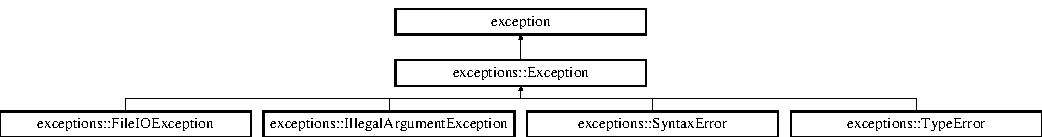
\includegraphics[height=1.842105cm]{d8/db2/classexceptions_1_1Exception}
\end{center}
\end{figure}
\subsection*{Public Member Functions}
\begin{DoxyCompactItemize}
\item 
\mbox{\Hypertarget{classexceptions_1_1Exception_a5cc4b7ff5b47b0cd72878380743ea1a0}\label{classexceptions_1_1Exception_a5cc4b7ff5b47b0cd72878380743ea1a0}} 
virtual const std\+::string {\bfseries get\+Message} () const
\item 
\mbox{\Hypertarget{classexceptions_1_1Exception_ad2d7459cc4eb53de89b453b0cac9330b}\label{classexceptions_1_1Exception_ad2d7459cc4eb53de89b453b0cac9330b}} 
virtual const std\+::string {\bfseries get\+Error} () const =0
\item 
\mbox{\Hypertarget{classexceptions_1_1Exception_ad51d6b57a9796fe4e28c3443a472ba21}\label{classexceptions_1_1Exception_ad51d6b57a9796fe4e28c3443a472ba21}} 
const char $\ast$ {\bfseries what} () const override  throw ()
\end{DoxyCompactItemize}
\subsection*{Protected Attributes}
\begin{DoxyCompactItemize}
\item 
\mbox{\Hypertarget{classexceptions_1_1Exception_a500171f957a84170c022fa1983eb47ee}\label{classexceptions_1_1Exception_a500171f957a84170c022fa1983eb47ee}} 
std\+::string {\bfseries message}
\end{DoxyCompactItemize}


The documentation for this class was generated from the following files\+:\begin{DoxyCompactItemize}
\item 
exceptions/\hyperlink{Exception_8h}{Exception.\+h}\item 
exceptions/\hyperlink{Exception_8cpp}{Exception.\+cpp}\end{DoxyCompactItemize}

\hypertarget{classexceptions_1_1FileIOException}{}\section{exceptions\+:\+:File\+I\+O\+Exception Class Reference}
\label{classexceptions_1_1FileIOException}\index{exceptions\+::\+File\+I\+O\+Exception@{exceptions\+::\+File\+I\+O\+Exception}}
Inheritance diagram for exceptions\+:\+:File\+I\+O\+Exception\+:\begin{figure}[H]
\begin{center}
\leavevmode
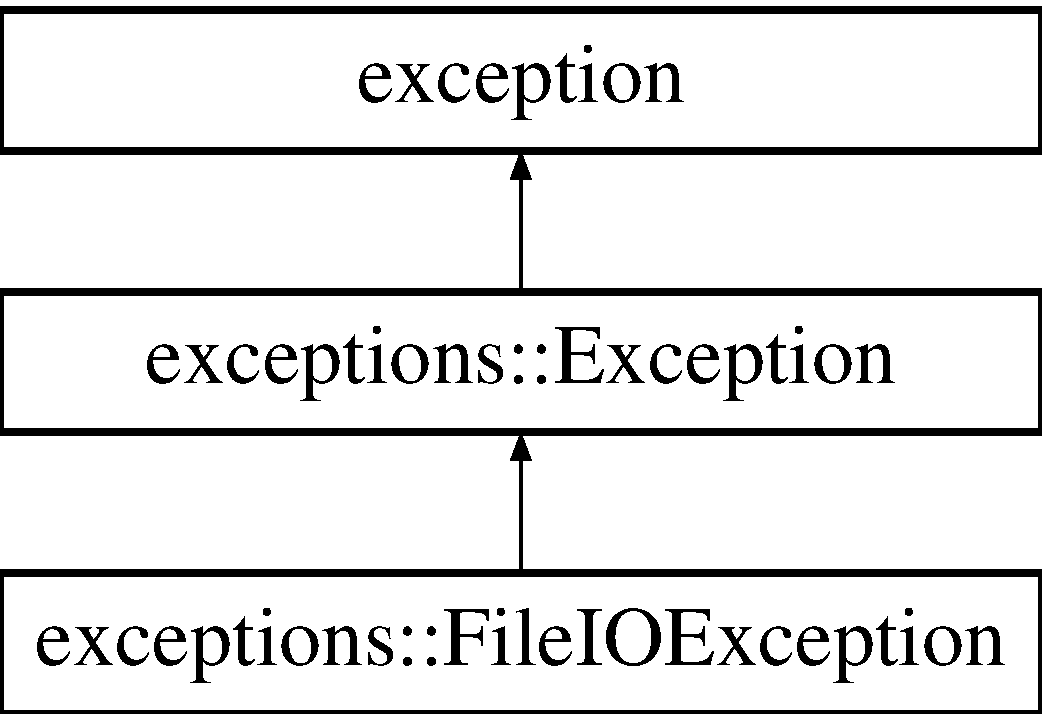
\includegraphics[height=3.000000cm]{d5/da9/classexceptions_1_1FileIOException}
\end{center}
\end{figure}
\subsection*{Public Member Functions}
\begin{DoxyCompactItemize}
\item 
\mbox{\Hypertarget{classexceptions_1_1FileIOException_ab561288a16a6e53e03304faa84442d8b}\label{classexceptions_1_1FileIOException_ab561288a16a6e53e03304faa84442d8b}} 
{\bfseries File\+I\+O\+Exception} (std\+::string message, std\+::string filename)
\item 
\mbox{\Hypertarget{classexceptions_1_1FileIOException_a9b1d1a131694d1e3c41b4d42fb11b449}\label{classexceptions_1_1FileIOException_a9b1d1a131694d1e3c41b4d42fb11b449}} 
const std\+::string {\bfseries get\+Filename} () const
\item 
\mbox{\Hypertarget{classexceptions_1_1FileIOException_a801fada59775c81ad5a2471f8bc5e360}\label{classexceptions_1_1FileIOException_a801fada59775c81ad5a2471f8bc5e360}} 
const std\+::string {\bfseries get\+Error} () const override
\end{DoxyCompactItemize}
\subsection*{Additional Inherited Members}


The documentation for this class was generated from the following files\+:\begin{DoxyCompactItemize}
\item 
exceptions/File\+I\+O\+Exception.\+h\item 
exceptions/File\+I\+O\+Exception.\+cpp\end{DoxyCompactItemize}

\hypertarget{classexceptions_1_1IllegalArgumentException}{}\section{exceptions\+:\+:Illegal\+Argument\+Exception Class Reference}
\label{classexceptions_1_1IllegalArgumentException}\index{exceptions\+::\+Illegal\+Argument\+Exception@{exceptions\+::\+Illegal\+Argument\+Exception}}


{\ttfamily \#include $<$Illegal\+Argument\+Exception.\+h$>$}

Inheritance diagram for exceptions\+:\+:Illegal\+Argument\+Exception\+:\begin{figure}[H]
\begin{center}
\leavevmode
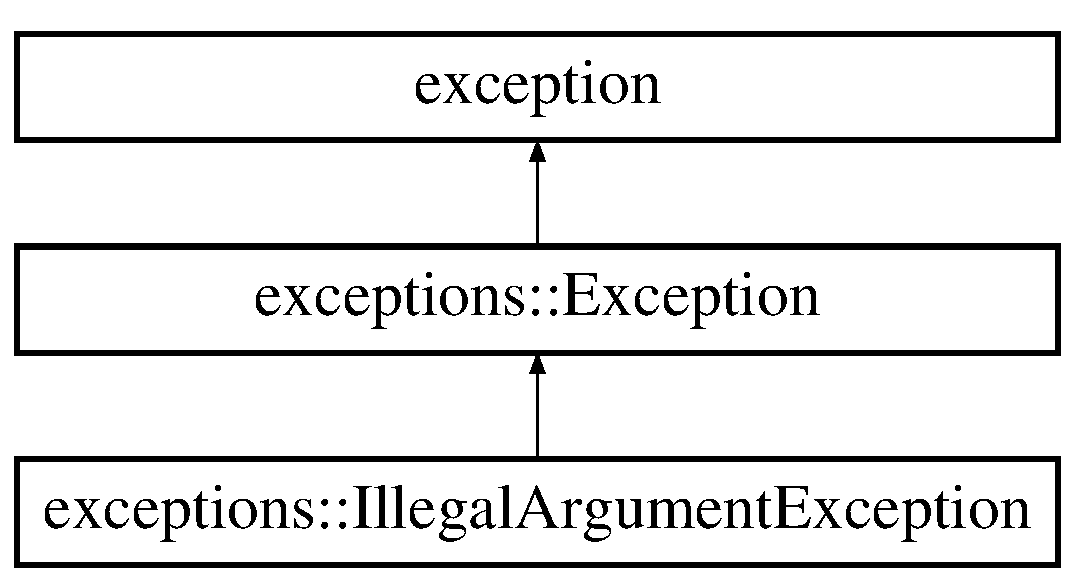
\includegraphics[height=3.000000cm]{de/d97/classexceptions_1_1IllegalArgumentException}
\end{center}
\end{figure}
\subsection*{Public Member Functions}
\begin{DoxyCompactItemize}
\item 
\hyperlink{classexceptions_1_1IllegalArgumentException_a299c4dc8ad0df639a618ced7799001ff}{Illegal\+Argument\+Exception} (const std\+::string message, const std\+::string \&argument)
\item 
const std\+::string \& \hyperlink{classexceptions_1_1IllegalArgumentException_a9228ab515c25921dc0e5c68e54fb2104}{get\+Argument} () const
\item 
const std\+::string \hyperlink{classexceptions_1_1IllegalArgumentException_aa11433daf8612e2730a0473f402d297a}{get\+Error} () const override
\end{DoxyCompactItemize}
\subsection*{Additional Inherited Members}


\subsection{Detailed Description}
\hyperlink{classexceptions_1_1Exception}{Exception} to show an illegal argument was given 

\subsection{Constructor \& Destructor Documentation}
\mbox{\Hypertarget{classexceptions_1_1IllegalArgumentException_a299c4dc8ad0df639a618ced7799001ff}\label{classexceptions_1_1IllegalArgumentException_a299c4dc8ad0df639a618ced7799001ff}} 
\index{exceptions\+::\+Illegal\+Argument\+Exception@{exceptions\+::\+Illegal\+Argument\+Exception}!Illegal\+Argument\+Exception@{Illegal\+Argument\+Exception}}
\index{Illegal\+Argument\+Exception@{Illegal\+Argument\+Exception}!exceptions\+::\+Illegal\+Argument\+Exception@{exceptions\+::\+Illegal\+Argument\+Exception}}
\subsubsection{\texorpdfstring{Illegal\+Argument\+Exception()}{IllegalArgumentException()}}
{\footnotesize\ttfamily exceptions\+::\+Illegal\+Argument\+Exception\+::\+Illegal\+Argument\+Exception (\begin{DoxyParamCaption}\item[{const std\+::string}]{message,  }\item[{const std\+::string \&}]{argument }\end{DoxyParamCaption})}

Constructor for this exception 
\begin{DoxyParams}{Parameters}
{\em message} & The error message \\
\hline
{\em argument} & The argument that\textquotesingle{}s raised the exception \\
\hline
\end{DoxyParams}


\subsection{Member Function Documentation}
\mbox{\Hypertarget{classexceptions_1_1IllegalArgumentException_a9228ab515c25921dc0e5c68e54fb2104}\label{classexceptions_1_1IllegalArgumentException_a9228ab515c25921dc0e5c68e54fb2104}} 
\index{exceptions\+::\+Illegal\+Argument\+Exception@{exceptions\+::\+Illegal\+Argument\+Exception}!get\+Argument@{get\+Argument}}
\index{get\+Argument@{get\+Argument}!exceptions\+::\+Illegal\+Argument\+Exception@{exceptions\+::\+Illegal\+Argument\+Exception}}
\subsubsection{\texorpdfstring{get\+Argument()}{getArgument()}}
{\footnotesize\ttfamily const std\+::string \& exceptions\+::\+Illegal\+Argument\+Exception\+::get\+Argument (\begin{DoxyParamCaption}{ }\end{DoxyParamCaption}) const}

\begin{DoxyReturn}{Returns}
The argument that raised the exception 
\end{DoxyReturn}
\mbox{\Hypertarget{classexceptions_1_1IllegalArgumentException_aa11433daf8612e2730a0473f402d297a}\label{classexceptions_1_1IllegalArgumentException_aa11433daf8612e2730a0473f402d297a}} 
\index{exceptions\+::\+Illegal\+Argument\+Exception@{exceptions\+::\+Illegal\+Argument\+Exception}!get\+Error@{get\+Error}}
\index{get\+Error@{get\+Error}!exceptions\+::\+Illegal\+Argument\+Exception@{exceptions\+::\+Illegal\+Argument\+Exception}}
\subsubsection{\texorpdfstring{get\+Error()}{getError()}}
{\footnotesize\ttfamily const std\+::string exceptions\+::\+Illegal\+Argument\+Exception\+::get\+Error (\begin{DoxyParamCaption}{ }\end{DoxyParamCaption}) const\hspace{0.3cm}{\ttfamily [override]}, {\ttfamily [virtual]}}

\begin{DoxyReturn}{Returns}
The full error message 
\end{DoxyReturn}


Implements \hyperlink{classexceptions_1_1Exception}{exceptions\+::\+Exception}.



The documentation for this class was generated from the following files\+:\begin{DoxyCompactItemize}
\item 
exceptions/\hyperlink{IllegalArgumentException_8h}{Illegal\+Argument\+Exception.\+h}\item 
exceptions/\hyperlink{IllegalArgumentException_8cpp}{Illegal\+Argument\+Exception.\+cpp}\end{DoxyCompactItemize}

\hypertarget{classvisitor_1_1InterpreterVisitor}{}\section{visitor\+:\+:Interpreter\+Visitor Class Reference}
\label{classvisitor_1_1InterpreterVisitor}\index{visitor\+::\+Interpreter\+Visitor@{visitor\+::\+Interpreter\+Visitor}}
Inheritance diagram for visitor\+:\+:Interpreter\+Visitor\+:\begin{figure}[H]
\begin{center}
\leavevmode
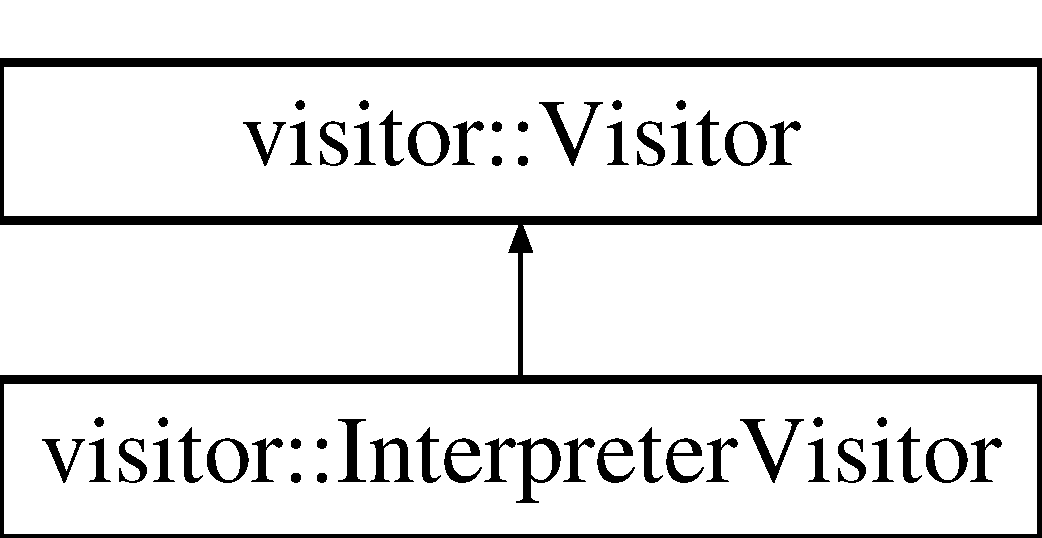
\includegraphics[height=2.000000cm]{d3/d91/classvisitor_1_1InterpreterVisitor}
\end{center}
\end{figure}
\subsection*{Public Member Functions}
\begin{DoxyCompactItemize}
\item 
\mbox{\Hypertarget{classvisitor_1_1InterpreterVisitor_a41fe83fe34750c37dffe4854eb0ad009}\label{classvisitor_1_1InterpreterVisitor_a41fe83fe34750c37dffe4854eb0ad009}} 
{\bfseries Interpreter\+Visitor} (const \hyperlink{classvisitor_1_1helper_1_1ScopedSymbolTable}{helper\+::\+Scoped\+Symbol\+Table} \&symbol\+Table, const \hyperlink{structvisitor_1_1helper_1_1Symbol}{helper\+::\+Symbol} \&stack\+Ans, bool is\+Return)
\item 
\mbox{\Hypertarget{classvisitor_1_1InterpreterVisitor_a82eb95cfdc93a496fac621cab4c8f81b}\label{classvisitor_1_1InterpreterVisitor_a82eb95cfdc93a496fac621cab4c8f81b}} 
void {\bfseries visit} (\hyperlink{classparser_1_1ast_1_1ASTExprNode}{parser\+::ast\+::\+A\+S\+T\+Expr\+Node} $\ast$node) override
\item 
\mbox{\Hypertarget{classvisitor_1_1InterpreterVisitor_acbaa5d4aead1a8f515e2dfb05cee5fc0}\label{classvisitor_1_1InterpreterVisitor_acbaa5d4aead1a8f515e2dfb05cee5fc0}} 
void {\bfseries visit} (\hyperlink{classparser_1_1ast_1_1ASTSimpleExprNode}{parser\+::ast\+::\+A\+S\+T\+Simple\+Expr\+Node} $\ast$node) override
\item 
\mbox{\Hypertarget{classvisitor_1_1InterpreterVisitor_a0fa4dac52a77eff5e233e0e3e36877fb}\label{classvisitor_1_1InterpreterVisitor_a0fa4dac52a77eff5e233e0e3e36877fb}} 
void {\bfseries visit} (\hyperlink{classparser_1_1ast_1_1ASTTermNode}{parser\+::ast\+::\+A\+S\+T\+Term\+Node} $\ast$node) override
\item 
\mbox{\Hypertarget{classvisitor_1_1InterpreterVisitor_adcc7dd80162847093191d9ba297b59be}\label{classvisitor_1_1InterpreterVisitor_adcc7dd80162847093191d9ba297b59be}} 
void {\bfseries visit} (\hyperlink{classparser_1_1ast_1_1ASTLiteralNode}{parser\+::ast\+::\+A\+S\+T\+Literal\+Node}$<$ int $>$ $\ast$node) override
\item 
\mbox{\Hypertarget{classvisitor_1_1InterpreterVisitor_a8020c5c81d73331c1f62a40c5379eab2}\label{classvisitor_1_1InterpreterVisitor_a8020c5c81d73331c1f62a40c5379eab2}} 
void {\bfseries visit} (\hyperlink{classparser_1_1ast_1_1ASTLiteralNode}{parser\+::ast\+::\+A\+S\+T\+Literal\+Node}$<$ float $>$ $\ast$node) override
\item 
\mbox{\Hypertarget{classvisitor_1_1InterpreterVisitor_a7354dfa5bc61a9a0772cd9bc97a21b1e}\label{classvisitor_1_1InterpreterVisitor_a7354dfa5bc61a9a0772cd9bc97a21b1e}} 
void {\bfseries visit} (\hyperlink{classparser_1_1ast_1_1ASTLiteralNode}{parser\+::ast\+::\+A\+S\+T\+Literal\+Node}$<$ bool $>$ $\ast$node) override
\item 
\mbox{\Hypertarget{classvisitor_1_1InterpreterVisitor_a19398633cd2c6170012b31ab6a409ddd}\label{classvisitor_1_1InterpreterVisitor_a19398633cd2c6170012b31ab6a409ddd}} 
void {\bfseries visit} (\hyperlink{classparser_1_1ast_1_1ASTLiteralNode}{parser\+::ast\+::\+A\+S\+T\+Literal\+Node}$<$ std\+::string $>$ $\ast$node) override
\item 
\mbox{\Hypertarget{classvisitor_1_1InterpreterVisitor_af4c36582bc131f24b21473a2ad3863e2}\label{classvisitor_1_1InterpreterVisitor_af4c36582bc131f24b21473a2ad3863e2}} 
void {\bfseries visit} (\hyperlink{classparser_1_1ast_1_1ASTFunctionCallNode}{parser\+::ast\+::\+A\+S\+T\+Function\+Call\+Node} $\ast$node) override
\item 
\mbox{\Hypertarget{classvisitor_1_1InterpreterVisitor_a74cc15ec03e36832293260a4d044a754}\label{classvisitor_1_1InterpreterVisitor_a74cc15ec03e36832293260a4d044a754}} 
void {\bfseries visit} (\hyperlink{classparser_1_1ast_1_1ASTIdentifierNode}{parser\+::ast\+::\+A\+S\+T\+Identifier\+Node} $\ast$node) override
\item 
\mbox{\Hypertarget{classvisitor_1_1InterpreterVisitor_a18bc942a7ebfcdaa5dad72c74217afbd}\label{classvisitor_1_1InterpreterVisitor_a18bc942a7ebfcdaa5dad72c74217afbd}} 
void {\bfseries visit} (\hyperlink{classparser_1_1ast_1_1ASTSubExpression}{parser\+::ast\+::\+A\+S\+T\+Sub\+Expression} $\ast$node) override
\item 
\mbox{\Hypertarget{classvisitor_1_1InterpreterVisitor_a78ae6427ebd645e999cca5633ed550a8}\label{classvisitor_1_1InterpreterVisitor_a78ae6427ebd645e999cca5633ed550a8}} 
void {\bfseries visit} (\hyperlink{classparser_1_1ast_1_1ASTUnaryNode}{parser\+::ast\+::\+A\+S\+T\+Unary\+Node} $\ast$node) override
\item 
\mbox{\Hypertarget{classvisitor_1_1InterpreterVisitor_a96c185b01435b7235556b4b8f143a7e9}\label{classvisitor_1_1InterpreterVisitor_a96c185b01435b7235556b4b8f143a7e9}} 
void {\bfseries visit} (\hyperlink{classparser_1_1ast_1_1ASTAssignmentNode}{parser\+::ast\+::\+A\+S\+T\+Assignment\+Node} $\ast$node) override
\item 
\mbox{\Hypertarget{classvisitor_1_1InterpreterVisitor_a0df27eef74e21ae2dfe5936cc2204fea}\label{classvisitor_1_1InterpreterVisitor_a0df27eef74e21ae2dfe5936cc2204fea}} 
void {\bfseries visit} (\hyperlink{classparser_1_1ast_1_1ASTVariableDeclStatementNode}{parser\+::ast\+::\+A\+S\+T\+Variable\+Decl\+Statement\+Node} $\ast$node) override
\item 
\mbox{\Hypertarget{classvisitor_1_1InterpreterVisitor_aaae681112d72ad284950bdae70fca289}\label{classvisitor_1_1InterpreterVisitor_aaae681112d72ad284950bdae70fca289}} 
void {\bfseries visit} (\hyperlink{classparser_1_1ast_1_1ASTBlockStatementNode}{parser\+::ast\+::\+A\+S\+T\+Block\+Statement\+Node} $\ast$node) override
\item 
\mbox{\Hypertarget{classvisitor_1_1InterpreterVisitor_a8794d5b1f7495b6a8530dfdd73e3ec3a}\label{classvisitor_1_1InterpreterVisitor_a8794d5b1f7495b6a8530dfdd73e3ec3a}} 
void {\bfseries visit} (\hyperlink{classparser_1_1ast_1_1ASTFunctionDeclStatementNode}{parser\+::ast\+::\+A\+S\+T\+Function\+Decl\+Statement\+Node} $\ast$node) override
\item 
\mbox{\Hypertarget{classvisitor_1_1InterpreterVisitor_a177f5f7515bd9ab07ad6c3792fb2591c}\label{classvisitor_1_1InterpreterVisitor_a177f5f7515bd9ab07ad6c3792fb2591c}} 
void {\bfseries visit} (\hyperlink{classparser_1_1ast_1_1ASTIfStatementNode}{parser\+::ast\+::\+A\+S\+T\+If\+Statement\+Node} $\ast$node) override
\item 
\mbox{\Hypertarget{classvisitor_1_1InterpreterVisitor_a25837b644b8527ec237445764c5c969a}\label{classvisitor_1_1InterpreterVisitor_a25837b644b8527ec237445764c5c969a}} 
void {\bfseries visit} (\hyperlink{classparser_1_1ast_1_1ASTWhileStatementNode}{parser\+::ast\+::\+A\+S\+T\+While\+Statement\+Node} $\ast$node) override
\item 
\mbox{\Hypertarget{classvisitor_1_1InterpreterVisitor_a82515caa4e94b97d1b229447ca26d634}\label{classvisitor_1_1InterpreterVisitor_a82515caa4e94b97d1b229447ca26d634}} 
void {\bfseries visit} (\hyperlink{classparser_1_1ast_1_1ASTPrintStatementNode}{parser\+::ast\+::\+A\+S\+T\+Print\+Statement\+Node} $\ast$node) override
\item 
\mbox{\Hypertarget{classvisitor_1_1InterpreterVisitor_a3bbe6812aea4b9b7221b99e078aa89a9}\label{classvisitor_1_1InterpreterVisitor_a3bbe6812aea4b9b7221b99e078aa89a9}} 
void {\bfseries visit} (\hyperlink{classparser_1_1ast_1_1ASTReturnStatementNode}{parser\+::ast\+::\+A\+S\+T\+Return\+Statement\+Node} $\ast$node) override
\item 
\mbox{\Hypertarget{classvisitor_1_1InterpreterVisitor_a31210bc4525068f9ee4e56b545814205}\label{classvisitor_1_1InterpreterVisitor_a31210bc4525068f9ee4e56b545814205}} 
void {\bfseries visit} (std\+::vector$<$ std\+::unique\+\_\+ptr$<$ \hyperlink{classparser_1_1ast_1_1ASTNode}{parser\+::ast\+::\+A\+S\+T\+Node} $>$$>$ \&nodes) override
\item 
\mbox{\Hypertarget{classvisitor_1_1InterpreterVisitor_a361da803df3ed71e0665b065439a69f0}\label{classvisitor_1_1InterpreterVisitor_a361da803df3ed71e0665b065439a69f0}} 
const \hyperlink{classvisitor_1_1helper_1_1ScopedSymbolTable}{helper\+::\+Scoped\+Symbol\+Table} \& {\bfseries get\+Symbol\+Table} () const
\end{DoxyCompactItemize}


The documentation for this class was generated from the following files\+:\begin{DoxyCompactItemize}
\item 
visitor/\hyperlink{InterpreterVisitor_8h}{Interpreter\+Visitor.\+h}\item 
visitor/\hyperlink{InterpreterVisitor_8cpp}{Interpreter\+Visitor.\+cpp}\end{DoxyCompactItemize}

\hypertarget{classlexer_1_1Lexer}{}\section{lexer\+:\+:Lexer Class Reference}
\label{classlexer_1_1Lexer}\index{lexer\+::\+Lexer@{lexer\+::\+Lexer}}


{\ttfamily \#include $<$Lexer.\+h$>$}

\subsection*{Public Member Functions}
\begin{DoxyCompactItemize}
\item 
\hyperlink{classlexer_1_1Lexer_aa41e05a67869b1ff8a9980af4e6ceb69}{Lexer} (std\+::vector$<$ std\+::string $>$ \&file\+\_\+contents)
\item 
\hyperlink{classlexer_1_1Token}{Token} \hyperlink{classlexer_1_1Lexer_ab44ae44ee3256fbc79b33a63b3b9bcde}{next\+Token} ()
\item 
std\+::pair$<$ int, int $>$ \hyperlink{classlexer_1_1Lexer_add05c7c77f92ad5a8f91123ecebec71d}{get\+Position} ()
\end{DoxyCompactItemize}


\subsection{Detailed Description}
This lexer acts as a D\+FA Note that this D\+FA is really an N\+FA, since the checks are those that are defined in A\+L\+P\+H\+A\+B\+E\+T\+\_\+\+P\+R\+E\+D\+I\+C\+A\+T\+ES. However, the order of these predicates is indeed a priority, starting from the highest to the lowest and as a result, the Finite-\/\+State Automata will not return more than one state, thus making it a deterministic. ` 

\subsection{Constructor \& Destructor Documentation}
\mbox{\Hypertarget{classlexer_1_1Lexer_aa41e05a67869b1ff8a9980af4e6ceb69}\label{classlexer_1_1Lexer_aa41e05a67869b1ff8a9980af4e6ceb69}} 
\index{lexer\+::\+Lexer@{lexer\+::\+Lexer}!Lexer@{Lexer}}
\index{Lexer@{Lexer}!lexer\+::\+Lexer@{lexer\+::\+Lexer}}
\subsubsection{\texorpdfstring{Lexer()}{Lexer()}}
{\footnotesize\ttfamily lexer\+::\+Lexer\+::\+Lexer (\begin{DoxyParamCaption}\item[{std\+::vector$<$ std\+::string $>$ \&}]{file\+\_\+contents }\end{DoxyParamCaption})}

Constructor with the file contents, useful for debugging purposes. 
\begin{DoxyParams}{Parameters}
{\em file\+\_\+contents} & The vector with the contents of the file. \\
\hline
\end{DoxyParams}


\subsection{Member Function Documentation}
\mbox{\Hypertarget{classlexer_1_1Lexer_add05c7c77f92ad5a8f91123ecebec71d}\label{classlexer_1_1Lexer_add05c7c77f92ad5a8f91123ecebec71d}} 
\index{lexer\+::\+Lexer@{lexer\+::\+Lexer}!get\+Position@{get\+Position}}
\index{get\+Position@{get\+Position}!lexer\+::\+Lexer@{lexer\+::\+Lexer}}
\subsubsection{\texorpdfstring{get\+Position()}{getPosition()}}
{\footnotesize\ttfamily std\+::pair$<$ int, int $>$ lexer\+::\+Lexer\+::get\+Position (\begin{DoxyParamCaption}{ }\end{DoxyParamCaption})}

Returns the current cursor position \begin{DoxyReturn}{Returns}
tuple containing integers as $<$row, col$>$ 
\end{DoxyReturn}
\mbox{\Hypertarget{classlexer_1_1Lexer_ab44ae44ee3256fbc79b33a63b3b9bcde}\label{classlexer_1_1Lexer_ab44ae44ee3256fbc79b33a63b3b9bcde}} 
\index{lexer\+::\+Lexer@{lexer\+::\+Lexer}!next\+Token@{next\+Token}}
\index{next\+Token@{next\+Token}!lexer\+::\+Lexer@{lexer\+::\+Lexer}}
\subsubsection{\texorpdfstring{next\+Token()}{nextToken()}}
{\footnotesize\ttfamily \hyperlink{classlexer_1_1Token}{lexer\+::\+Token} lexer\+::\+Lexer\+::next\+Token (\begin{DoxyParamCaption}{ }\end{DoxyParamCaption})}

Returns the next token that was found from the file contnets. \begin{DoxyReturn}{Returns}
T\+He next \hyperlink{classlexer_1_1Token}{Token} to be parsed.
\end{DoxyReturn}
A tail recursive approach was taken to avoid accessing memory after the end of the vector \begin{DoxyReturn}{Returns}
The next token 
\end{DoxyReturn}

\begin{DoxyExceptions}{Exceptions}
{\em Syntax\+Error} & if the lexer is unable to parse the next token. \\
\hline
\end{DoxyExceptions}


The documentation for this class was generated from the following files\+:\begin{DoxyCompactItemize}
\item 
lexer/\hyperlink{Lexer_8h}{Lexer.\+h}\item 
lexer/Lexer.\+cpp\end{DoxyCompactItemize}

\hypertarget{classparser_1_1Parser}{}\section{parser\+:\+:Parser Class Reference}
\label{classparser_1_1Parser}\index{parser\+::\+Parser@{parser\+::\+Parser}}
\subsection*{Public Member Functions}
\begin{DoxyCompactItemize}
\item 
\mbox{\Hypertarget{classparser_1_1Parser_a18234ace1965274d1ff87ab837e8e919}\label{classparser_1_1Parser_a18234ace1965274d1ff87ab837e8e919}} 
{\bfseries Parser} (std\+::vector$<$ std\+::string $>$ \&lines)
\item 
std\+::vector$<$ std\+::unique\+\_\+ptr$<$ \hyperlink{classparser_1_1ast_1_1ASTNode}{ast\+::\+A\+S\+T\+Node} $>$ $>$ \hyperlink{classparser_1_1Parser_afc66d21a0a64957f0d982026c319b80e}{parse} ()
\end{DoxyCompactItemize}


\subsection{Member Function Documentation}
\mbox{\Hypertarget{classparser_1_1Parser_afc66d21a0a64957f0d982026c319b80e}\label{classparser_1_1Parser_afc66d21a0a64957f0d982026c319b80e}} 
\index{parser\+::\+Parser@{parser\+::\+Parser}!parse@{parse}}
\index{parse@{parse}!parser\+::\+Parser@{parser\+::\+Parser}}
\subsubsection{\texorpdfstring{parse()}{parse()}}
{\footnotesize\ttfamily std\+::vector$<$ std\+::unique\+\_\+ptr$<$ \hyperlink{classparser_1_1ast_1_1ASTNode}{parser\+::ast\+::\+A\+S\+T\+Node} $>$ $>$ parser\+::\+Parser\+::parse (\begin{DoxyParamCaption}{ }\end{DoxyParamCaption})}

\begin{DoxyReturn}{Returns}
a (sort of abstract) root node in the form of a vector of nodes 
\end{DoxyReturn}


The documentation for this class was generated from the following files\+:\begin{DoxyCompactItemize}
\item 
parser/Parser.\+h\item 
parser/Parser.\+cpp\end{DoxyCompactItemize}

\hypertarget{structlexer_1_1Position}{}\section{lexer\+:\+:Position Struct Reference}
\label{structlexer_1_1Position}\index{lexer\+::\+Position@{lexer\+::\+Position}}


{\ttfamily \#include $<$Lexer.\+h$>$}

\subsection*{Public Attributes}
\begin{DoxyCompactItemize}
\item 
\mbox{\Hypertarget{structlexer_1_1Position_a04c39fe571e9afc8dad6f659ab2271f6}\label{structlexer_1_1Position_a04c39fe571e9afc8dad6f659ab2271f6}} 
std\+::vector$<$ std\+::string $>$\+::iterator {\bfseries line}
\item 
\mbox{\Hypertarget{structlexer_1_1Position_a3a02b3f6c6aaa411bb6845389283cc23}\label{structlexer_1_1Position_a3a02b3f6c6aaa411bb6845389283cc23}} 
std\+::string\+::iterator {\bfseries character}
\item 
\mbox{\Hypertarget{structlexer_1_1Position_a1b457b24326fd14c91d156b0148cabdf}\label{structlexer_1_1Position_a1b457b24326fd14c91d156b0148cabdf}} 
std\+::string {\bfseries chars\+\_\+read}
\end{DoxyCompactItemize}


\subsection{Detailed Description}
This struct represents the cursor used to read the file input 

The documentation for this struct was generated from the following file\+:\begin{DoxyCompactItemize}
\item 
lexer/\hyperlink{Lexer_8h}{Lexer.\+h}\end{DoxyCompactItemize}

\hypertarget{classvisitor_1_1helper_1_1ScopedSymbolTable}{}\section{visitor\+:\+:helper\+:\+:Scoped\+Symbol\+Table Class Reference}
\label{classvisitor_1_1helper_1_1ScopedSymbolTable}\index{visitor\+::helper\+::\+Scoped\+Symbol\+Table@{visitor\+::helper\+::\+Scoped\+Symbol\+Table}}
\subsection*{Public Member Functions}
\begin{DoxyCompactItemize}
\item 
void \hyperlink{classvisitor_1_1helper_1_1ScopedSymbolTable_afa14e4f8f1b71fe6961120f55c20c50c}{add\+Entry\+To\+Symbol\+Table} (std\+::string identifier, \hyperlink{ASTVariableDeclStatementNode_8h_a1e8e1bde0729627e3a22ffa858d5f3b9}{Symbol\+Type} type)
\item 
void \hyperlink{classvisitor_1_1helper_1_1ScopedSymbolTable_afc5afd4fe70ae4556e512db38c9c257b}{add\+Entry\+To\+Symbol\+Table} (std\+::string identifier, int int\+Value)
\item 
void \hyperlink{classvisitor_1_1helper_1_1ScopedSymbolTable_a8297b38007e89b53bb8286b7afd23d37}{add\+Entry\+To\+Symbol\+Table} (std\+::string identifier, float real\+Value)
\item 
void \hyperlink{classvisitor_1_1helper_1_1ScopedSymbolTable_a4161155b0e73f398bb816a92895f5099}{add\+Entry\+To\+Symbol\+Table} (std\+::string identifier, bool bool\+Value)
\item 
void \hyperlink{classvisitor_1_1helper_1_1ScopedSymbolTable_ad9531010cb89b1fc09e4850894c957a2}{add\+Entry\+To\+Symbol\+Table} (std\+::string identifier, std\+::string string\+Value)
\item 
void \hyperlink{classvisitor_1_1helper_1_1ScopedSymbolTable_a7bd90ed126440e1110882ef00b8095ce}{add\+Entry\+To\+Symbol\+Table} (std\+::string identifier, \hyperlink{classparser_1_1ast_1_1ASTFunctionDeclStatementNode}{parser\+::ast\+::\+A\+S\+T\+Function\+Decl\+Statement\+Node} $\ast$function\+Decl\+Statement\+Node)
\item 
void \hyperlink{classvisitor_1_1helper_1_1ScopedSymbolTable_a7b1027f36d0682ea440d48230f7ec62a}{add\+Entry\+To\+Symbol\+Table} (std\+::string identifier, \hyperlink{structvisitor_1_1helper_1_1Symbol}{Symbol} value)
\item 
void \hyperlink{classvisitor_1_1helper_1_1ScopedSymbolTable_a4938e3fb5c563484363538994a080be8}{add\+Scope} ()
\item 
void \hyperlink{classvisitor_1_1helper_1_1ScopedSymbolTable_afbeb4833a967d03a31f00306b5c21eb1}{pop\+Scope} ()
\item 
bool \hyperlink{classvisitor_1_1helper_1_1ScopedSymbolTable_a173eb4fb447dfcc8f8eaedfffeb7ae97}{check\+Symbol\+Exists} (std\+::string identifier)
\item 
\hyperlink{structvisitor_1_1helper_1_1Symbol}{Symbol} \hyperlink{classvisitor_1_1helper_1_1ScopedSymbolTable_a30038c7ddf4e21666d163d3f41382ff1}{get\+Symbol} (std\+::string identifier)
\item 
void \hyperlink{classvisitor_1_1helper_1_1ScopedSymbolTable_aaacddfaa8cb0843ba2821bd898270a1a}{change\+Symbol\+Value} (std\+::string identifier, \hyperlink{structvisitor_1_1helper_1_1Symbol}{Symbol} value)
\item 
\mbox{\Hypertarget{classvisitor_1_1helper_1_1ScopedSymbolTable_a52b16de9cb62ca65654e2ceb97bda9b4}\label{classvisitor_1_1helper_1_1ScopedSymbolTable_a52b16de9cb62ca65654e2ceb97bda9b4}} 
const std\+::vector$<$ std\+::unique\+\_\+ptr$<$ std\+::map$<$ std\+::string, \hyperlink{structvisitor_1_1helper_1_1Symbol}{Symbol} $>$ $>$ $>$ \& {\bfseries get\+Symbol\+Table} () const
\end{DoxyCompactItemize}


\subsection{Member Function Documentation}
\mbox{\Hypertarget{classvisitor_1_1helper_1_1ScopedSymbolTable_afa14e4f8f1b71fe6961120f55c20c50c}\label{classvisitor_1_1helper_1_1ScopedSymbolTable_afa14e4f8f1b71fe6961120f55c20c50c}} 
\index{visitor\+::helper\+::\+Scoped\+Symbol\+Table@{visitor\+::helper\+::\+Scoped\+Symbol\+Table}!add\+Entry\+To\+Symbol\+Table@{add\+Entry\+To\+Symbol\+Table}}
\index{add\+Entry\+To\+Symbol\+Table@{add\+Entry\+To\+Symbol\+Table}!visitor\+::helper\+::\+Scoped\+Symbol\+Table@{visitor\+::helper\+::\+Scoped\+Symbol\+Table}}
\subsubsection{\texorpdfstring{add\+Entry\+To\+Symbol\+Table()}{addEntryToSymbolTable()}\hspace{0.1cm}{\footnotesize\ttfamily [1/7]}}
{\footnotesize\ttfamily void visitor\+::helper\+::\+Scoped\+Symbol\+Table\+::add\+Entry\+To\+Symbol\+Table (\begin{DoxyParamCaption}\item[{std\+::string}]{identifier,  }\item[{\hyperlink{ASTVariableDeclStatementNode_8h_a1e8e1bde0729627e3a22ffa858d5f3b9}{Symbol\+Type}}]{type }\end{DoxyParamCaption})}

Adds an entry to the symbol table at the last scope created. 
\begin{DoxyParams}{Parameters}
{\em identifier} & the identifier to add \\
\hline
{\em type} & the identifier\textquotesingle{}s type. if this is a function, it must be the return type. \\
\hline
\end{DoxyParams}
\mbox{\Hypertarget{classvisitor_1_1helper_1_1ScopedSymbolTable_afc5afd4fe70ae4556e512db38c9c257b}\label{classvisitor_1_1helper_1_1ScopedSymbolTable_afc5afd4fe70ae4556e512db38c9c257b}} 
\index{visitor\+::helper\+::\+Scoped\+Symbol\+Table@{visitor\+::helper\+::\+Scoped\+Symbol\+Table}!add\+Entry\+To\+Symbol\+Table@{add\+Entry\+To\+Symbol\+Table}}
\index{add\+Entry\+To\+Symbol\+Table@{add\+Entry\+To\+Symbol\+Table}!visitor\+::helper\+::\+Scoped\+Symbol\+Table@{visitor\+::helper\+::\+Scoped\+Symbol\+Table}}
\subsubsection{\texorpdfstring{add\+Entry\+To\+Symbol\+Table()}{addEntryToSymbolTable()}\hspace{0.1cm}{\footnotesize\ttfamily [2/7]}}
{\footnotesize\ttfamily void visitor\+::helper\+::\+Scoped\+Symbol\+Table\+::add\+Entry\+To\+Symbol\+Table (\begin{DoxyParamCaption}\item[{std\+::string}]{identifier,  }\item[{int}]{int\+Value }\end{DoxyParamCaption})}

Adds an entry to the symbol table at the last scope created. 
\begin{DoxyParams}{Parameters}
{\em identifier} & the identifier to add \\
\hline
{\em int\+Value} & the integer value \\
\hline
\end{DoxyParams}
\mbox{\Hypertarget{classvisitor_1_1helper_1_1ScopedSymbolTable_a8297b38007e89b53bb8286b7afd23d37}\label{classvisitor_1_1helper_1_1ScopedSymbolTable_a8297b38007e89b53bb8286b7afd23d37}} 
\index{visitor\+::helper\+::\+Scoped\+Symbol\+Table@{visitor\+::helper\+::\+Scoped\+Symbol\+Table}!add\+Entry\+To\+Symbol\+Table@{add\+Entry\+To\+Symbol\+Table}}
\index{add\+Entry\+To\+Symbol\+Table@{add\+Entry\+To\+Symbol\+Table}!visitor\+::helper\+::\+Scoped\+Symbol\+Table@{visitor\+::helper\+::\+Scoped\+Symbol\+Table}}
\subsubsection{\texorpdfstring{add\+Entry\+To\+Symbol\+Table()}{addEntryToSymbolTable()}\hspace{0.1cm}{\footnotesize\ttfamily [3/7]}}
{\footnotesize\ttfamily void visitor\+::helper\+::\+Scoped\+Symbol\+Table\+::add\+Entry\+To\+Symbol\+Table (\begin{DoxyParamCaption}\item[{std\+::string}]{identifier,  }\item[{float}]{real\+Value }\end{DoxyParamCaption})}

Adds an entry to the symbol table at the last scope created. 
\begin{DoxyParams}{Parameters}
{\em identifier} & the identifier to add \\
\hline
{\em real\+Value} & the real value \\
\hline
\end{DoxyParams}
\mbox{\Hypertarget{classvisitor_1_1helper_1_1ScopedSymbolTable_a4161155b0e73f398bb816a92895f5099}\label{classvisitor_1_1helper_1_1ScopedSymbolTable_a4161155b0e73f398bb816a92895f5099}} 
\index{visitor\+::helper\+::\+Scoped\+Symbol\+Table@{visitor\+::helper\+::\+Scoped\+Symbol\+Table}!add\+Entry\+To\+Symbol\+Table@{add\+Entry\+To\+Symbol\+Table}}
\index{add\+Entry\+To\+Symbol\+Table@{add\+Entry\+To\+Symbol\+Table}!visitor\+::helper\+::\+Scoped\+Symbol\+Table@{visitor\+::helper\+::\+Scoped\+Symbol\+Table}}
\subsubsection{\texorpdfstring{add\+Entry\+To\+Symbol\+Table()}{addEntryToSymbolTable()}\hspace{0.1cm}{\footnotesize\ttfamily [4/7]}}
{\footnotesize\ttfamily void visitor\+::helper\+::\+Scoped\+Symbol\+Table\+::add\+Entry\+To\+Symbol\+Table (\begin{DoxyParamCaption}\item[{std\+::string}]{identifier,  }\item[{bool}]{bool\+Value }\end{DoxyParamCaption})}

Adds an entry to the symbol table at the last scope created. 
\begin{DoxyParams}{Parameters}
{\em identifier} & the identifier to add \\
\hline
{\em bool\+Value} & the Boolean Value \\
\hline
\end{DoxyParams}
\mbox{\Hypertarget{classvisitor_1_1helper_1_1ScopedSymbolTable_ad9531010cb89b1fc09e4850894c957a2}\label{classvisitor_1_1helper_1_1ScopedSymbolTable_ad9531010cb89b1fc09e4850894c957a2}} 
\index{visitor\+::helper\+::\+Scoped\+Symbol\+Table@{visitor\+::helper\+::\+Scoped\+Symbol\+Table}!add\+Entry\+To\+Symbol\+Table@{add\+Entry\+To\+Symbol\+Table}}
\index{add\+Entry\+To\+Symbol\+Table@{add\+Entry\+To\+Symbol\+Table}!visitor\+::helper\+::\+Scoped\+Symbol\+Table@{visitor\+::helper\+::\+Scoped\+Symbol\+Table}}
\subsubsection{\texorpdfstring{add\+Entry\+To\+Symbol\+Table()}{addEntryToSymbolTable()}\hspace{0.1cm}{\footnotesize\ttfamily [5/7]}}
{\footnotesize\ttfamily void visitor\+::helper\+::\+Scoped\+Symbol\+Table\+::add\+Entry\+To\+Symbol\+Table (\begin{DoxyParamCaption}\item[{std\+::string}]{identifier,  }\item[{std\+::string}]{string\+Value }\end{DoxyParamCaption})}

Adds an entry to the symbol table at the last scope created. 
\begin{DoxyParams}{Parameters}
{\em identifier} & the identifier to add \\
\hline
{\em string\+Value} & the string value \\
\hline
\end{DoxyParams}
\mbox{\Hypertarget{classvisitor_1_1helper_1_1ScopedSymbolTable_a7bd90ed126440e1110882ef00b8095ce}\label{classvisitor_1_1helper_1_1ScopedSymbolTable_a7bd90ed126440e1110882ef00b8095ce}} 
\index{visitor\+::helper\+::\+Scoped\+Symbol\+Table@{visitor\+::helper\+::\+Scoped\+Symbol\+Table}!add\+Entry\+To\+Symbol\+Table@{add\+Entry\+To\+Symbol\+Table}}
\index{add\+Entry\+To\+Symbol\+Table@{add\+Entry\+To\+Symbol\+Table}!visitor\+::helper\+::\+Scoped\+Symbol\+Table@{visitor\+::helper\+::\+Scoped\+Symbol\+Table}}
\subsubsection{\texorpdfstring{add\+Entry\+To\+Symbol\+Table()}{addEntryToSymbolTable()}\hspace{0.1cm}{\footnotesize\ttfamily [6/7]}}
{\footnotesize\ttfamily void visitor\+::helper\+::\+Scoped\+Symbol\+Table\+::add\+Entry\+To\+Symbol\+Table (\begin{DoxyParamCaption}\item[{std\+::string}]{identifier,  }\item[{\hyperlink{classparser_1_1ast_1_1ASTFunctionDeclStatementNode}{parser\+::ast\+::\+A\+S\+T\+Function\+Decl\+Statement\+Node} $\ast$}]{function\+Decl\+Statement\+Node }\end{DoxyParamCaption})}

Adds an entry to the symbol table at the last scope created when the type is unknown but given to be correct 
\begin{DoxyParams}{Parameters}
{\em identifier} & the identifier to add \\
\hline
{\em value} & the value \\
\hline
\end{DoxyParams}
\mbox{\Hypertarget{classvisitor_1_1helper_1_1ScopedSymbolTable_a7b1027f36d0682ea440d48230f7ec62a}\label{classvisitor_1_1helper_1_1ScopedSymbolTable_a7b1027f36d0682ea440d48230f7ec62a}} 
\index{visitor\+::helper\+::\+Scoped\+Symbol\+Table@{visitor\+::helper\+::\+Scoped\+Symbol\+Table}!add\+Entry\+To\+Symbol\+Table@{add\+Entry\+To\+Symbol\+Table}}
\index{add\+Entry\+To\+Symbol\+Table@{add\+Entry\+To\+Symbol\+Table}!visitor\+::helper\+::\+Scoped\+Symbol\+Table@{visitor\+::helper\+::\+Scoped\+Symbol\+Table}}
\subsubsection{\texorpdfstring{add\+Entry\+To\+Symbol\+Table()}{addEntryToSymbolTable()}\hspace{0.1cm}{\footnotesize\ttfamily [7/7]}}
{\footnotesize\ttfamily void visitor\+::helper\+::\+Scoped\+Symbol\+Table\+::add\+Entry\+To\+Symbol\+Table (\begin{DoxyParamCaption}\item[{std\+::string}]{identifier,  }\item[{\hyperlink{structvisitor_1_1helper_1_1Symbol}{Symbol}}]{value }\end{DoxyParamCaption})}

Adds an entry to the symbol table at the last scope created when the type is unknown but given to be correct 
\begin{DoxyParams}{Parameters}
{\em identifier} & the identifier to add \\
\hline
{\em value} & the value \\
\hline
\end{DoxyParams}
\mbox{\Hypertarget{classvisitor_1_1helper_1_1ScopedSymbolTable_a4938e3fb5c563484363538994a080be8}\label{classvisitor_1_1helper_1_1ScopedSymbolTable_a4938e3fb5c563484363538994a080be8}} 
\index{visitor\+::helper\+::\+Scoped\+Symbol\+Table@{visitor\+::helper\+::\+Scoped\+Symbol\+Table}!add\+Scope@{add\+Scope}}
\index{add\+Scope@{add\+Scope}!visitor\+::helper\+::\+Scoped\+Symbol\+Table@{visitor\+::helper\+::\+Scoped\+Symbol\+Table}}
\subsubsection{\texorpdfstring{add\+Scope()}{addScope()}}
{\footnotesize\ttfamily void visitor\+::helper\+::\+Scoped\+Symbol\+Table\+::add\+Scope (\begin{DoxyParamCaption}{ }\end{DoxyParamCaption})}

Adds a scope and creates a symbol table for it \begin{DoxyReturn}{Returns}
true if sucessful, false otherwise 
\end{DoxyReturn}
\mbox{\Hypertarget{classvisitor_1_1helper_1_1ScopedSymbolTable_aaacddfaa8cb0843ba2821bd898270a1a}\label{classvisitor_1_1helper_1_1ScopedSymbolTable_aaacddfaa8cb0843ba2821bd898270a1a}} 
\index{visitor\+::helper\+::\+Scoped\+Symbol\+Table@{visitor\+::helper\+::\+Scoped\+Symbol\+Table}!change\+Symbol\+Value@{change\+Symbol\+Value}}
\index{change\+Symbol\+Value@{change\+Symbol\+Value}!visitor\+::helper\+::\+Scoped\+Symbol\+Table@{visitor\+::helper\+::\+Scoped\+Symbol\+Table}}
\subsubsection{\texorpdfstring{change\+Symbol\+Value()}{changeSymbolValue()}}
{\footnotesize\ttfamily void visitor\+::helper\+::\+Scoped\+Symbol\+Table\+::change\+Symbol\+Value (\begin{DoxyParamCaption}\item[{std\+::string}]{identifier,  }\item[{\hyperlink{structvisitor_1_1helper_1_1Symbol}{Symbol}}]{value }\end{DoxyParamCaption})}

Changes an entry to the symbol table at the last scope it was created 
\begin{DoxyParams}{Parameters}
{\em identifier} & the identifier to change \\
\hline
{\em value} & the value \\
\hline
\end{DoxyParams}
\mbox{\Hypertarget{classvisitor_1_1helper_1_1ScopedSymbolTable_a173eb4fb447dfcc8f8eaedfffeb7ae97}\label{classvisitor_1_1helper_1_1ScopedSymbolTable_a173eb4fb447dfcc8f8eaedfffeb7ae97}} 
\index{visitor\+::helper\+::\+Scoped\+Symbol\+Table@{visitor\+::helper\+::\+Scoped\+Symbol\+Table}!check\+Symbol\+Exists@{check\+Symbol\+Exists}}
\index{check\+Symbol\+Exists@{check\+Symbol\+Exists}!visitor\+::helper\+::\+Scoped\+Symbol\+Table@{visitor\+::helper\+::\+Scoped\+Symbol\+Table}}
\subsubsection{\texorpdfstring{check\+Symbol\+Exists()}{checkSymbolExists()}}
{\footnotesize\ttfamily bool visitor\+::helper\+::\+Scoped\+Symbol\+Table\+::check\+Symbol\+Exists (\begin{DoxyParamCaption}\item[{std\+::string}]{identifier }\end{DoxyParamCaption})}

Checks whether the identifier given exists or not \begin{DoxyReturn}{Returns}
true if the identifier is found, false otherwise 
\end{DoxyReturn}
\mbox{\Hypertarget{classvisitor_1_1helper_1_1ScopedSymbolTable_a30038c7ddf4e21666d163d3f41382ff1}\label{classvisitor_1_1helper_1_1ScopedSymbolTable_a30038c7ddf4e21666d163d3f41382ff1}} 
\index{visitor\+::helper\+::\+Scoped\+Symbol\+Table@{visitor\+::helper\+::\+Scoped\+Symbol\+Table}!get\+Symbol@{get\+Symbol}}
\index{get\+Symbol@{get\+Symbol}!visitor\+::helper\+::\+Scoped\+Symbol\+Table@{visitor\+::helper\+::\+Scoped\+Symbol\+Table}}
\subsubsection{\texorpdfstring{get\+Symbol()}{getSymbol()}}
{\footnotesize\ttfamily \hyperlink{structvisitor_1_1helper_1_1Symbol}{visitor\+::helper\+::\+Symbol} visitor\+::helper\+::\+Scoped\+Symbol\+Table\+::get\+Symbol (\begin{DoxyParamCaption}\item[{std\+::string}]{identifier }\end{DoxyParamCaption})}

Gets the type of the symbol. Throws a Type\+Error if the symbol is not found. \begin{DoxyReturn}{Returns}
the Symbol\+Type of the identifier 
\end{DoxyReturn}
\mbox{\Hypertarget{classvisitor_1_1helper_1_1ScopedSymbolTable_afbeb4833a967d03a31f00306b5c21eb1}\label{classvisitor_1_1helper_1_1ScopedSymbolTable_afbeb4833a967d03a31f00306b5c21eb1}} 
\index{visitor\+::helper\+::\+Scoped\+Symbol\+Table@{visitor\+::helper\+::\+Scoped\+Symbol\+Table}!pop\+Scope@{pop\+Scope}}
\index{pop\+Scope@{pop\+Scope}!visitor\+::helper\+::\+Scoped\+Symbol\+Table@{visitor\+::helper\+::\+Scoped\+Symbol\+Table}}
\subsubsection{\texorpdfstring{pop\+Scope()}{popScope()}}
{\footnotesize\ttfamily void visitor\+::helper\+::\+Scoped\+Symbol\+Table\+::pop\+Scope (\begin{DoxyParamCaption}{ }\end{DoxyParamCaption})}

Removes the last scope from this symbol table, and all it\textquotesingle{}s symbols 

The documentation for this class was generated from the following files\+:\begin{DoxyCompactItemize}
\item 
visitor/helpers/\hyperlink{ScopedSymbolTable_8h}{Scoped\+Symbol\+Table.\+h}\item 
visitor/helpers/\hyperlink{ScopedSymbolTable_8cpp}{Scoped\+Symbol\+Table.\+cpp}\end{DoxyCompactItemize}

\hypertarget{structvisitor_1_1helper_1_1Symbol}{}\section{visitor\+:\+:helper\+:\+:Symbol Struct Reference}
\label{structvisitor_1_1helper_1_1Symbol}\index{visitor\+::helper\+::\+Symbol@{visitor\+::helper\+::\+Symbol}}
\subsection*{Classes}
\begin{DoxyCompactItemize}
\item 
union \hyperlink{unionvisitor_1_1helper_1_1Symbol_1_1Value}{Value}
\end{DoxyCompactItemize}
\subsection*{Public Member Functions}
\begin{DoxyCompactItemize}
\item 
\mbox{\Hypertarget{structvisitor_1_1helper_1_1Symbol_ad32b28990e36de9ca8bcb64a9775c255}\label{structvisitor_1_1helper_1_1Symbol_ad32b28990e36de9ca8bcb64a9775c255}} 
{\bfseries Symbol} (W\+H\+I\+C\+H\+\_\+\+V\+A\+L\+UE value\+Type, \hyperlink{unionvisitor_1_1helper_1_1Symbol_1_1Value}{Value} value)
\item 
\mbox{\Hypertarget{structvisitor_1_1helper_1_1Symbol_a2f447584c211d452dc0fe79b80c2ca2c}\label{structvisitor_1_1helper_1_1Symbol_a2f447584c211d452dc0fe79b80c2ca2c}} 
{\bfseries Symbol} (\hyperlink{ASTVariableDeclStatementNode_8h_a1e8e1bde0729627e3a22ffa858d5f3b9}{Symbol\+Type} value)
\item 
\mbox{\Hypertarget{structvisitor_1_1helper_1_1Symbol_a12aa40b952eaa6a64b148ff3dc6ad88a}\label{structvisitor_1_1helper_1_1Symbol_a12aa40b952eaa6a64b148ff3dc6ad88a}} 
{\bfseries Symbol} (int value)
\item 
\mbox{\Hypertarget{structvisitor_1_1helper_1_1Symbol_ae05fe0ccd5e107992b07f5939811dbb0}\label{structvisitor_1_1helper_1_1Symbol_ae05fe0ccd5e107992b07f5939811dbb0}} 
{\bfseries Symbol} (bool value)
\item 
\mbox{\Hypertarget{structvisitor_1_1helper_1_1Symbol_a8ed20173f3a8d4f3f28517170b8f3c6e}\label{structvisitor_1_1helper_1_1Symbol_a8ed20173f3a8d4f3f28517170b8f3c6e}} 
{\bfseries Symbol} (float value)
\item 
\mbox{\Hypertarget{structvisitor_1_1helper_1_1Symbol_a88580214c3b94b1a4585b02ae3efe6bf}\label{structvisitor_1_1helper_1_1Symbol_a88580214c3b94b1a4585b02ae3efe6bf}} 
{\bfseries Symbol} (std\+::string $\ast$value)
\item 
\mbox{\Hypertarget{structvisitor_1_1helper_1_1Symbol_a06a4138c8b736f8ed7e3878abfe44f93}\label{structvisitor_1_1helper_1_1Symbol_a06a4138c8b736f8ed7e3878abfe44f93}} 
{\bfseries Symbol} (\hyperlink{classparser_1_1ast_1_1ASTFunctionDeclStatementNode}{parser\+::ast\+::\+A\+S\+T\+Function\+Decl\+Statement\+Node} $\ast$value)
\end{DoxyCompactItemize}
\subsection*{Public Attributes}
\begin{DoxyCompactItemize}
\item 
\mbox{\Hypertarget{structvisitor_1_1helper_1_1Symbol_aebb6af7f12ef493c13e092b9e0072456}\label{structvisitor_1_1helper_1_1Symbol_aebb6af7f12ef493c13e092b9e0072456}} 
W\+H\+I\+C\+H\+\_\+\+V\+A\+L\+UE {\bfseries value\+Type}
\item 
\mbox{\Hypertarget{structvisitor_1_1helper_1_1Symbol_a406184b57090559b32bb06ffc7717324}\label{structvisitor_1_1helper_1_1Symbol_a406184b57090559b32bb06ffc7717324}} 
union \hyperlink{unionvisitor_1_1helper_1_1Symbol_1_1Value}{visitor\+::helper\+::\+Symbol\+::\+Value} {\bfseries value}
\end{DoxyCompactItemize}


The documentation for this struct was generated from the following file\+:\begin{DoxyCompactItemize}
\item 
visitor/helpers/\hyperlink{Symbol_8h}{Symbol.\+h}\end{DoxyCompactItemize}

\hypertarget{classexceptions_1_1SyntaxError}{}\section{exceptions\+:\+:Syntax\+Error Class Reference}
\label{classexceptions_1_1SyntaxError}\index{exceptions\+::\+Syntax\+Error@{exceptions\+::\+Syntax\+Error}}


{\ttfamily \#include $<$Syntax\+Error.\+h$>$}

Inheritance diagram for exceptions\+:\+:Syntax\+Error\+:\begin{figure}[H]
\begin{center}
\leavevmode
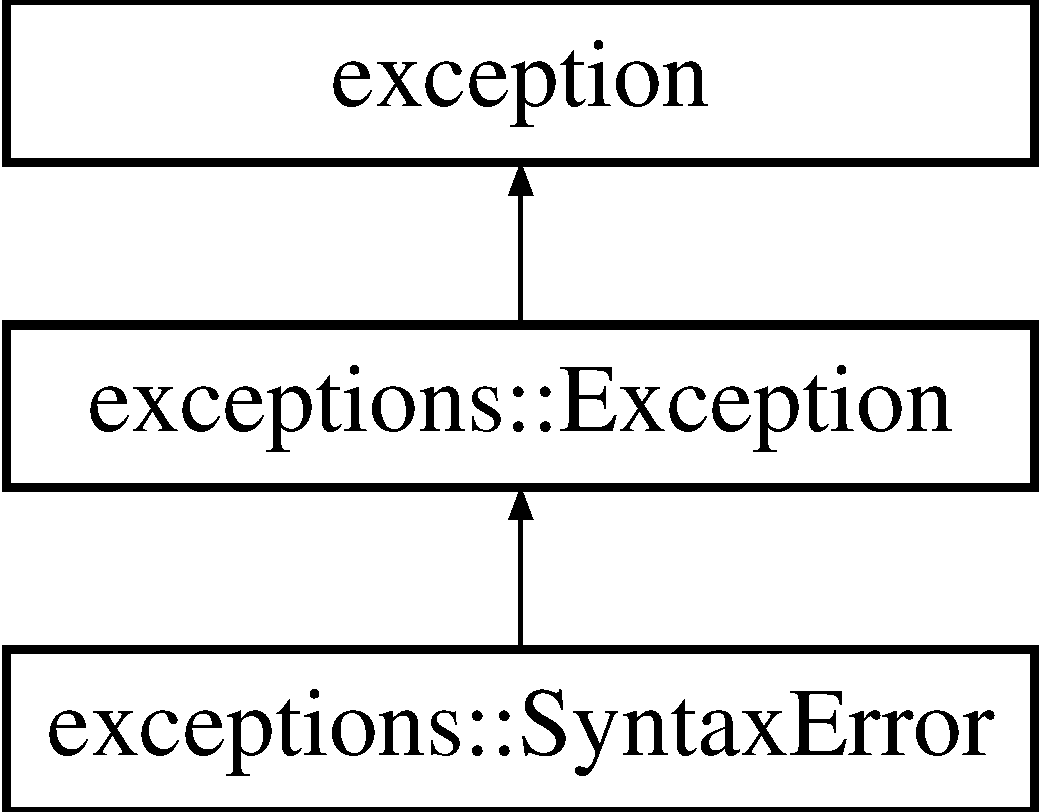
\includegraphics[height=3.000000cm]{d3/df7/classexceptions_1_1SyntaxError}
\end{center}
\end{figure}
\subsection*{Public Member Functions}
\begin{DoxyCompactItemize}
\item 
\hyperlink{classexceptions_1_1SyntaxError_ad47c8f8926f591f2d7a2d7e8a7c044a1}{Syntax\+Error} (const std\+::string message, long line\+No, long char\+No)
\item 
long \hyperlink{classexceptions_1_1SyntaxError_a250a5032a546390f979c3ff624a88ead}{get\+Line\+No} () const
\item 
long \hyperlink{classexceptions_1_1SyntaxError_aac30c99ba9e1f9cf75505c7150a72230}{get\+Char\+No} () const
\item 
const std\+::string \hyperlink{classexceptions_1_1SyntaxError_a76804893bdba149c9dc7df4f26be31e0}{get\+Error} () const override
\end{DoxyCompactItemize}
\subsection*{Additional Inherited Members}


\subsection{Detailed Description}
An exception that would be thrown if the lexer is unable to tokenize a lexeme This is also thrown if the parser can\textquotesingle{}t parse the token 

\subsection{Constructor \& Destructor Documentation}
\mbox{\Hypertarget{classexceptions_1_1SyntaxError_ad47c8f8926f591f2d7a2d7e8a7c044a1}\label{classexceptions_1_1SyntaxError_ad47c8f8926f591f2d7a2d7e8a7c044a1}} 
\index{exceptions\+::\+Syntax\+Error@{exceptions\+::\+Syntax\+Error}!Syntax\+Error@{Syntax\+Error}}
\index{Syntax\+Error@{Syntax\+Error}!exceptions\+::\+Syntax\+Error@{exceptions\+::\+Syntax\+Error}}
\subsubsection{\texorpdfstring{Syntax\+Error()}{SyntaxError()}}
{\footnotesize\ttfamily exceptions\+::\+Syntax\+Error\+::\+Syntax\+Error (\begin{DoxyParamCaption}\item[{const std\+::string}]{message,  }\item[{long}]{line\+No,  }\item[{long}]{char\+No }\end{DoxyParamCaption})}

Constructor for this exception 
\begin{DoxyParams}{Parameters}
{\em message} & The error message \\
\hline
{\em line\+No} & The line number where this syntax error occurred \\
\hline
{\em char\+No} & The character number where this syntax error occurred \\
\hline
\end{DoxyParams}


\subsection{Member Function Documentation}
\mbox{\Hypertarget{classexceptions_1_1SyntaxError_aac30c99ba9e1f9cf75505c7150a72230}\label{classexceptions_1_1SyntaxError_aac30c99ba9e1f9cf75505c7150a72230}} 
\index{exceptions\+::\+Syntax\+Error@{exceptions\+::\+Syntax\+Error}!get\+Char\+No@{get\+Char\+No}}
\index{get\+Char\+No@{get\+Char\+No}!exceptions\+::\+Syntax\+Error@{exceptions\+::\+Syntax\+Error}}
\subsubsection{\texorpdfstring{get\+Char\+No()}{getCharNo()}}
{\footnotesize\ttfamily long exceptions\+::\+Syntax\+Error\+::get\+Char\+No (\begin{DoxyParamCaption}{ }\end{DoxyParamCaption}) const}

\begin{DoxyReturn}{Returns}
The character number this error occurred 
\end{DoxyReturn}
\mbox{\Hypertarget{classexceptions_1_1SyntaxError_a76804893bdba149c9dc7df4f26be31e0}\label{classexceptions_1_1SyntaxError_a76804893bdba149c9dc7df4f26be31e0}} 
\index{exceptions\+::\+Syntax\+Error@{exceptions\+::\+Syntax\+Error}!get\+Error@{get\+Error}}
\index{get\+Error@{get\+Error}!exceptions\+::\+Syntax\+Error@{exceptions\+::\+Syntax\+Error}}
\subsubsection{\texorpdfstring{get\+Error()}{getError()}}
{\footnotesize\ttfamily const std\+::string exceptions\+::\+Syntax\+Error\+::get\+Error (\begin{DoxyParamCaption}{ }\end{DoxyParamCaption}) const\hspace{0.3cm}{\ttfamily [override]}, {\ttfamily [virtual]}}

\begin{DoxyReturn}{Returns}
The full error message (message + position) 
\end{DoxyReturn}


Implements \hyperlink{classexceptions_1_1Exception}{exceptions\+::\+Exception}.

\mbox{\Hypertarget{classexceptions_1_1SyntaxError_a250a5032a546390f979c3ff624a88ead}\label{classexceptions_1_1SyntaxError_a250a5032a546390f979c3ff624a88ead}} 
\index{exceptions\+::\+Syntax\+Error@{exceptions\+::\+Syntax\+Error}!get\+Line\+No@{get\+Line\+No}}
\index{get\+Line\+No@{get\+Line\+No}!exceptions\+::\+Syntax\+Error@{exceptions\+::\+Syntax\+Error}}
\subsubsection{\texorpdfstring{get\+Line\+No()}{getLineNo()}}
{\footnotesize\ttfamily long exceptions\+::\+Syntax\+Error\+::get\+Line\+No (\begin{DoxyParamCaption}{ }\end{DoxyParamCaption}) const}

\begin{DoxyReturn}{Returns}
The line number this error occurred 
\end{DoxyReturn}


The documentation for this class was generated from the following files\+:\begin{DoxyCompactItemize}
\item 
exceptions/\hyperlink{SyntaxError_8h}{Syntax\+Error.\+h}\item 
exceptions/Syntax\+Error.\+cpp\end{DoxyCompactItemize}

\hypertarget{classlexer_1_1Token}{}\section{lexer\+:\+:Token Class Reference}
\label{classlexer_1_1Token}\index{lexer\+::\+Token@{lexer\+::\+Token}}


{\ttfamily \#include $<$Token\+Type.\+h$>$}

\subsection*{Public Member Functions}
\begin{DoxyCompactItemize}
\item 
\hyperlink{classlexer_1_1Token_a1957043fccf9ff5053e2d16da91da677}{Token} (\hyperlink{TokenType_8h_a8609501a650c2bf52e8397c88de5770f}{Token\+Type} token, const std\+::string \&value)
\item 
\hyperlink{TokenType_8h_a8609501a650c2bf52e8397c88de5770f}{Token\+Type} \hyperlink{classlexer_1_1Token_a8375087ce4b276ed175ab3d171f76fd1}{get\+Token} () const
\item 
const std\+::string \& \hyperlink{classlexer_1_1Token_a6b50f258588b97a8087edf17ec3f2762}{get\+Attribute} () const
\end{DoxyCompactItemize}


\subsection{Detailed Description}
\hyperlink{classlexer_1_1Token}{Token} class that stores the enum \hyperlink{classlexer_1_1Token}{Token} and the attribute that made up this token. This could be a value, identifier etc... 

\subsection{Constructor \& Destructor Documentation}
\mbox{\Hypertarget{classlexer_1_1Token_a1957043fccf9ff5053e2d16da91da677}\label{classlexer_1_1Token_a1957043fccf9ff5053e2d16da91da677}} 
\index{lexer\+::\+Token@{lexer\+::\+Token}!Token@{Token}}
\index{Token@{Token}!lexer\+::\+Token@{lexer\+::\+Token}}
\subsubsection{\texorpdfstring{Token()}{Token()}}
{\footnotesize\ttfamily lexer\+::\+Token\+::\+Token (\begin{DoxyParamCaption}\item[{\hyperlink{TokenType_8h_a8609501a650c2bf52e8397c88de5770f}{lexer\+::\+Token\+Type}}]{token,  }\item[{const std\+::string \&}]{value }\end{DoxyParamCaption})}


\begin{DoxyParams}{Parameters}
{\em token} & The token type \\
\hline
{\em value} & The attribute that made up this token \\
\hline
\end{DoxyParams}


\subsection{Member Function Documentation}
\mbox{\Hypertarget{classlexer_1_1Token_a6b50f258588b97a8087edf17ec3f2762}\label{classlexer_1_1Token_a6b50f258588b97a8087edf17ec3f2762}} 
\index{lexer\+::\+Token@{lexer\+::\+Token}!get\+Attribute@{get\+Attribute}}
\index{get\+Attribute@{get\+Attribute}!lexer\+::\+Token@{lexer\+::\+Token}}
\subsubsection{\texorpdfstring{get\+Attribute()}{getAttribute()}}
{\footnotesize\ttfamily const std\+::string \& lexer\+::\+Token\+::get\+Attribute (\begin{DoxyParamCaption}{ }\end{DoxyParamCaption}) const}

\begin{DoxyReturn}{Returns}
The attribute 
\end{DoxyReturn}
\mbox{\Hypertarget{classlexer_1_1Token_a8375087ce4b276ed175ab3d171f76fd1}\label{classlexer_1_1Token_a8375087ce4b276ed175ab3d171f76fd1}} 
\index{lexer\+::\+Token@{lexer\+::\+Token}!get\+Token@{get\+Token}}
\index{get\+Token@{get\+Token}!lexer\+::\+Token@{lexer\+::\+Token}}
\subsubsection{\texorpdfstring{get\+Token()}{getToken()}}
{\footnotesize\ttfamily \hyperlink{TokenType_8h_a8609501a650c2bf52e8397c88de5770f}{lexer\+::\+Token\+Type} lexer\+::\+Token\+::get\+Token (\begin{DoxyParamCaption}{ }\end{DoxyParamCaption}) const}

\begin{DoxyReturn}{Returns}
The token 
\end{DoxyReturn}


The documentation for this class was generated from the following files\+:\begin{DoxyCompactItemize}
\item 
lexer/\hyperlink{TokenType_8h}{Token\+Type.\+h}\item 
lexer/Token\+Type.\+cpp\end{DoxyCompactItemize}

\hypertarget{classvisitor_1_1TypeCheckVisitor}{}\section{visitor\+:\+:Type\+Check\+Visitor Class Reference}
\label{classvisitor_1_1TypeCheckVisitor}\index{visitor\+::\+Type\+Check\+Visitor@{visitor\+::\+Type\+Check\+Visitor}}
Inheritance diagram for visitor\+:\+:Type\+Check\+Visitor\+:\begin{figure}[H]
\begin{center}
\leavevmode
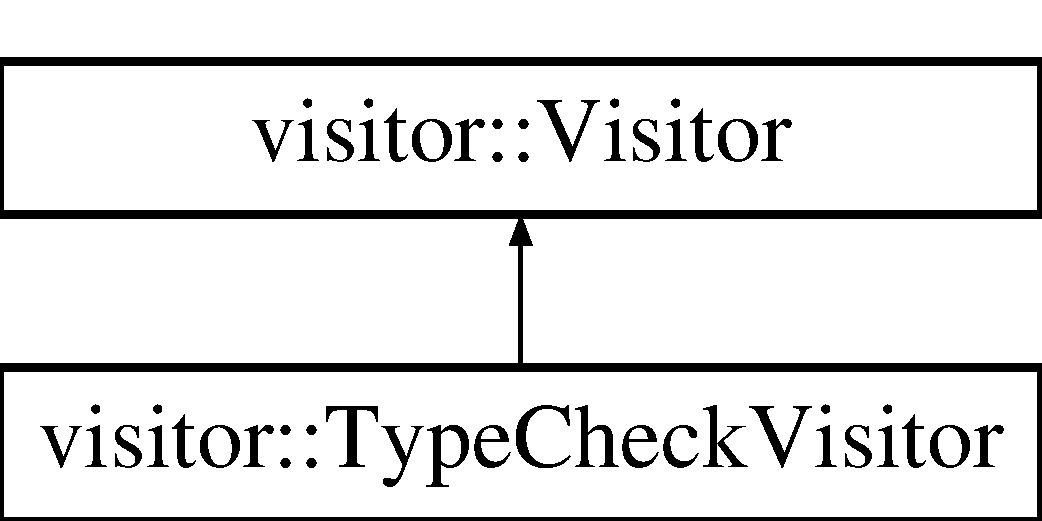
\includegraphics[height=2.000000cm]{d8/d91/classvisitor_1_1TypeCheckVisitor}
\end{center}
\end{figure}
\subsection*{Public Member Functions}
\begin{DoxyCompactItemize}
\item 
\mbox{\Hypertarget{classvisitor_1_1TypeCheckVisitor_aec4ad72e42bc34b577a572ba86aefec2}\label{classvisitor_1_1TypeCheckVisitor_aec4ad72e42bc34b577a572ba86aefec2}} 
void {\bfseries visit} (\hyperlink{classparser_1_1ast_1_1ASTExprNode}{parser\+::ast\+::\+A\+S\+T\+Expr\+Node} $\ast$node) override
\item 
\mbox{\Hypertarget{classvisitor_1_1TypeCheckVisitor_a8d7f1a19314471061a645de2cfca53be}\label{classvisitor_1_1TypeCheckVisitor_a8d7f1a19314471061a645de2cfca53be}} 
void {\bfseries visit} (\hyperlink{classparser_1_1ast_1_1ASTSimpleExprNode}{parser\+::ast\+::\+A\+S\+T\+Simple\+Expr\+Node} $\ast$node) override
\item 
\mbox{\Hypertarget{classvisitor_1_1TypeCheckVisitor_a5265a68e6f20e4de224044ef6d5156c4}\label{classvisitor_1_1TypeCheckVisitor_a5265a68e6f20e4de224044ef6d5156c4}} 
void {\bfseries visit} (\hyperlink{classparser_1_1ast_1_1ASTTermNode}{parser\+::ast\+::\+A\+S\+T\+Term\+Node} $\ast$node) override
\item 
\mbox{\Hypertarget{classvisitor_1_1TypeCheckVisitor_a1da13df9f4a67246e4fab28590b4ce3b}\label{classvisitor_1_1TypeCheckVisitor_a1da13df9f4a67246e4fab28590b4ce3b}} 
void {\bfseries visit} (\hyperlink{classparser_1_1ast_1_1ASTLiteralNode}{parser\+::ast\+::\+A\+S\+T\+Literal\+Node}$<$ int $>$ $\ast$node) override
\item 
\mbox{\Hypertarget{classvisitor_1_1TypeCheckVisitor_afd12a2144b14553195c594cc163fc4ca}\label{classvisitor_1_1TypeCheckVisitor_afd12a2144b14553195c594cc163fc4ca}} 
void {\bfseries visit} (\hyperlink{classparser_1_1ast_1_1ASTLiteralNode}{parser\+::ast\+::\+A\+S\+T\+Literal\+Node}$<$ float $>$ $\ast$node) override
\item 
\mbox{\Hypertarget{classvisitor_1_1TypeCheckVisitor_abaa1ff6899f3bd7156a613dee01fad37}\label{classvisitor_1_1TypeCheckVisitor_abaa1ff6899f3bd7156a613dee01fad37}} 
void {\bfseries visit} (\hyperlink{classparser_1_1ast_1_1ASTLiteralNode}{parser\+::ast\+::\+A\+S\+T\+Literal\+Node}$<$ bool $>$ $\ast$node) override
\item 
\mbox{\Hypertarget{classvisitor_1_1TypeCheckVisitor_a41e215d0be02b7532375d9d4a70c95d8}\label{classvisitor_1_1TypeCheckVisitor_a41e215d0be02b7532375d9d4a70c95d8}} 
void {\bfseries visit} (\hyperlink{classparser_1_1ast_1_1ASTLiteralNode}{parser\+::ast\+::\+A\+S\+T\+Literal\+Node}$<$ std\+::string $>$ $\ast$node) override
\item 
\mbox{\Hypertarget{classvisitor_1_1TypeCheckVisitor_a5b88cca44543546844e7a7ac1ee58040}\label{classvisitor_1_1TypeCheckVisitor_a5b88cca44543546844e7a7ac1ee58040}} 
void {\bfseries visit} (\hyperlink{classparser_1_1ast_1_1ASTFunctionCallNode}{parser\+::ast\+::\+A\+S\+T\+Function\+Call\+Node} $\ast$node) override
\item 
\mbox{\Hypertarget{classvisitor_1_1TypeCheckVisitor_a03914f91e3c36b34e6a3997c72e70d29}\label{classvisitor_1_1TypeCheckVisitor_a03914f91e3c36b34e6a3997c72e70d29}} 
void {\bfseries visit} (\hyperlink{classparser_1_1ast_1_1ASTIdentifierNode}{parser\+::ast\+::\+A\+S\+T\+Identifier\+Node} $\ast$node) override
\item 
\mbox{\Hypertarget{classvisitor_1_1TypeCheckVisitor_a3d58da29b8f7cce7193cbc2621d5eb37}\label{classvisitor_1_1TypeCheckVisitor_a3d58da29b8f7cce7193cbc2621d5eb37}} 
void {\bfseries visit} (\hyperlink{classparser_1_1ast_1_1ASTSubExpression}{parser\+::ast\+::\+A\+S\+T\+Sub\+Expression} $\ast$node) override
\item 
\mbox{\Hypertarget{classvisitor_1_1TypeCheckVisitor_a7c54f52ae31b9db1c9a2ac5da86d70f1}\label{classvisitor_1_1TypeCheckVisitor_a7c54f52ae31b9db1c9a2ac5da86d70f1}} 
void {\bfseries visit} (\hyperlink{classparser_1_1ast_1_1ASTUnaryNode}{parser\+::ast\+::\+A\+S\+T\+Unary\+Node} $\ast$node) override
\item 
\mbox{\Hypertarget{classvisitor_1_1TypeCheckVisitor_a57cc8b70f6972d9a2c03905d7bec7d04}\label{classvisitor_1_1TypeCheckVisitor_a57cc8b70f6972d9a2c03905d7bec7d04}} 
void {\bfseries visit} (\hyperlink{classparser_1_1ast_1_1ASTAssignmentNode}{parser\+::ast\+::\+A\+S\+T\+Assignment\+Node} $\ast$node) override
\item 
\mbox{\Hypertarget{classvisitor_1_1TypeCheckVisitor_ae78a97199c8c76ca1fe9ae9c4dd75120}\label{classvisitor_1_1TypeCheckVisitor_ae78a97199c8c76ca1fe9ae9c4dd75120}} 
void {\bfseries visit} (\hyperlink{classparser_1_1ast_1_1ASTVariableDeclStatementNode}{parser\+::ast\+::\+A\+S\+T\+Variable\+Decl\+Statement\+Node} $\ast$node) override
\item 
\mbox{\Hypertarget{classvisitor_1_1TypeCheckVisitor_aae83871964a35297a2c95e2f98842030}\label{classvisitor_1_1TypeCheckVisitor_aae83871964a35297a2c95e2f98842030}} 
void {\bfseries visit} (\hyperlink{classparser_1_1ast_1_1ASTBlockStatementNode}{parser\+::ast\+::\+A\+S\+T\+Block\+Statement\+Node} $\ast$node) override
\item 
\mbox{\Hypertarget{classvisitor_1_1TypeCheckVisitor_ae9fcfff8179c45778d710bd21b73200e}\label{classvisitor_1_1TypeCheckVisitor_ae9fcfff8179c45778d710bd21b73200e}} 
void {\bfseries visit} (\hyperlink{classparser_1_1ast_1_1ASTFunctionDeclStatementNode}{parser\+::ast\+::\+A\+S\+T\+Function\+Decl\+Statement\+Node} $\ast$node) override
\item 
\mbox{\Hypertarget{classvisitor_1_1TypeCheckVisitor_aa1b9cb2bd491d8935a50ebbccbd6924f}\label{classvisitor_1_1TypeCheckVisitor_aa1b9cb2bd491d8935a50ebbccbd6924f}} 
void {\bfseries visit} (\hyperlink{classparser_1_1ast_1_1ASTIfStatementNode}{parser\+::ast\+::\+A\+S\+T\+If\+Statement\+Node} $\ast$node) override
\item 
\mbox{\Hypertarget{classvisitor_1_1TypeCheckVisitor_a12b12e28530f7583c06bd1c81d985bb6}\label{classvisitor_1_1TypeCheckVisitor_a12b12e28530f7583c06bd1c81d985bb6}} 
void {\bfseries visit} (\hyperlink{classparser_1_1ast_1_1ASTWhileStatementNode}{parser\+::ast\+::\+A\+S\+T\+While\+Statement\+Node} $\ast$node) override
\item 
\mbox{\Hypertarget{classvisitor_1_1TypeCheckVisitor_a8b5c1e82bf98754ad0002d103d78f18c}\label{classvisitor_1_1TypeCheckVisitor_a8b5c1e82bf98754ad0002d103d78f18c}} 
void {\bfseries visit} (\hyperlink{classparser_1_1ast_1_1ASTPrintStatementNode}{parser\+::ast\+::\+A\+S\+T\+Print\+Statement\+Node} $\ast$node) override
\item 
\mbox{\Hypertarget{classvisitor_1_1TypeCheckVisitor_a308b8168805e875e55afcf2702fd4a31}\label{classvisitor_1_1TypeCheckVisitor_a308b8168805e875e55afcf2702fd4a31}} 
void {\bfseries visit} (\hyperlink{classparser_1_1ast_1_1ASTReturnStatementNode}{parser\+::ast\+::\+A\+S\+T\+Return\+Statement\+Node} $\ast$node) override
\item 
\mbox{\Hypertarget{classvisitor_1_1TypeCheckVisitor_a2c643169fd31a00116ae3cc45c5faec4}\label{classvisitor_1_1TypeCheckVisitor_a2c643169fd31a00116ae3cc45c5faec4}} 
void {\bfseries visit} (std\+::vector$<$ std\+::unique\+\_\+ptr$<$ \hyperlink{classparser_1_1ast_1_1ASTNode}{parser\+::ast\+::\+A\+S\+T\+Node} $>$$>$ \&nodes) override
\end{DoxyCompactItemize}


The documentation for this class was generated from the following files\+:\begin{DoxyCompactItemize}
\item 
visitor/\hyperlink{TypeCheckVisitor_8h}{Type\+Check\+Visitor.\+h}\item 
visitor/\hyperlink{TypeCheckVisitor_8cpp}{Type\+Check\+Visitor.\+cpp}\end{DoxyCompactItemize}

\hypertarget{classexceptions_1_1TypeError}{}\section{exceptions\+:\+:Type\+Error Class Reference}
\label{classexceptions_1_1TypeError}\index{exceptions\+::\+Type\+Error@{exceptions\+::\+Type\+Error}}
Inheritance diagram for exceptions\+:\+:Type\+Error\+:\begin{figure}[H]
\begin{center}
\leavevmode
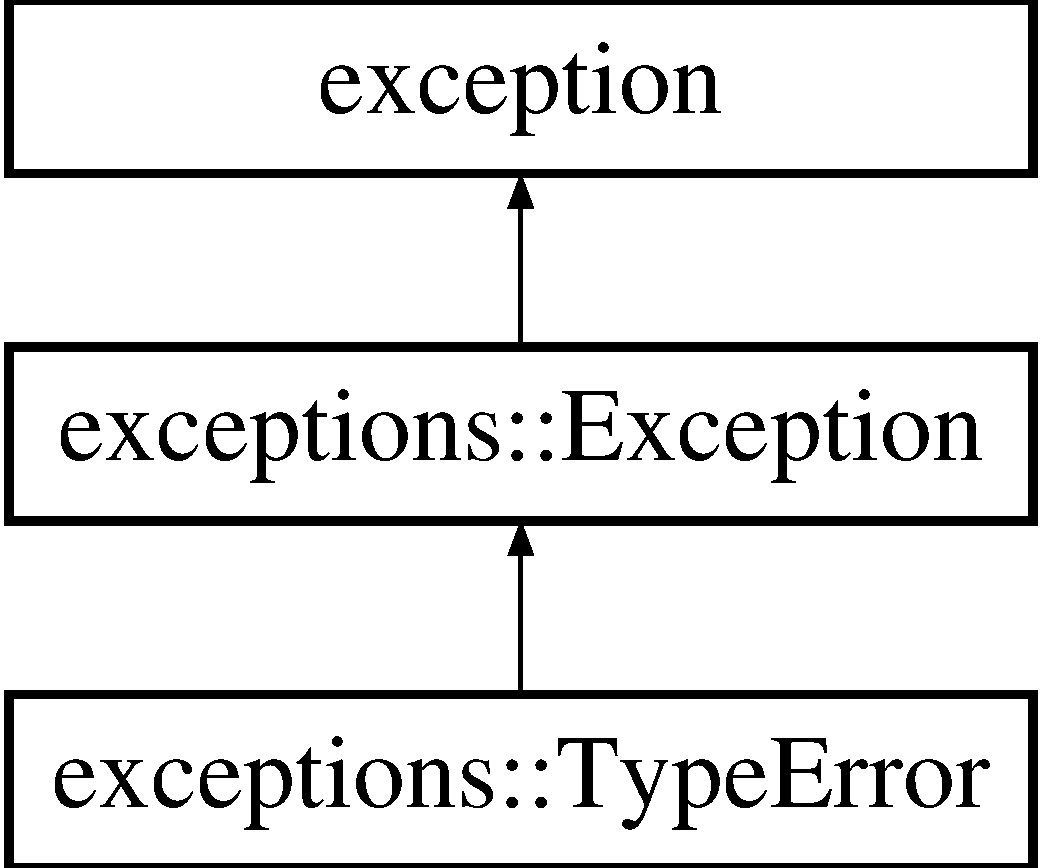
\includegraphics[height=3.000000cm]{dd/d31/classexceptions_1_1TypeError}
\end{center}
\end{figure}
\subsection*{Public Member Functions}
\begin{DoxyCompactItemize}
\item 
\mbox{\Hypertarget{classexceptions_1_1TypeError_a397aaaf8636c5accf7ccf04fa6e5fba4}\label{classexceptions_1_1TypeError_a397aaaf8636c5accf7ccf04fa6e5fba4}} 
{\bfseries Type\+Error} (const std\+::string message, const std\+::string identifier)
\item 
\mbox{\Hypertarget{classexceptions_1_1TypeError_a5f9ec99f11ad6fe3e4975f01503965e6}\label{classexceptions_1_1TypeError_a5f9ec99f11ad6fe3e4975f01503965e6}} 
{\bfseries Type\+Error} (const std\+::string message)
\item 
\mbox{\Hypertarget{classexceptions_1_1TypeError_a4efc952ccf7500b4ddd0e1df72609051}\label{classexceptions_1_1TypeError_a4efc952ccf7500b4ddd0e1df72609051}} 
const std\+::string \& {\bfseries get\+Identifier} () const
\item 
const std\+::string \hyperlink{classexceptions_1_1TypeError_aea887128840ec0cab163fe3272418542}{get\+Error} () const override
\end{DoxyCompactItemize}
\subsection*{Additional Inherited Members}


\subsection{Member Function Documentation}
\mbox{\Hypertarget{classexceptions_1_1TypeError_aea887128840ec0cab163fe3272418542}\label{classexceptions_1_1TypeError_aea887128840ec0cab163fe3272418542}} 
\index{exceptions\+::\+Type\+Error@{exceptions\+::\+Type\+Error}!get\+Error@{get\+Error}}
\index{get\+Error@{get\+Error}!exceptions\+::\+Type\+Error@{exceptions\+::\+Type\+Error}}
\subsubsection{\texorpdfstring{get\+Error()}{getError()}}
{\footnotesize\ttfamily const std\+::string exceptions\+::\+Type\+Error\+::get\+Error (\begin{DoxyParamCaption}{ }\end{DoxyParamCaption}) const\hspace{0.3cm}{\ttfamily [override]}, {\ttfamily [virtual]}}

\begin{DoxyReturn}{Returns}
The full error message (message + identifier) 
\end{DoxyReturn}


Implements \hyperlink{classexceptions_1_1Exception}{exceptions\+::\+Exception}.



The documentation for this class was generated from the following files\+:\begin{DoxyCompactItemize}
\item 
exceptions/\hyperlink{TypeError_8h}{Type\+Error.\+h}\item 
exceptions/\hyperlink{TypeError_8cpp}{Type\+Error.\+cpp}\end{DoxyCompactItemize}

\hypertarget{unionvisitor_1_1helper_1_1Symbol_1_1Value}{}\section{visitor\+:\+:helper\+:\+:Symbol\+:\+:Value Union Reference}
\label{unionvisitor_1_1helper_1_1Symbol_1_1Value}\index{visitor\+::helper\+::\+Symbol\+::\+Value@{visitor\+::helper\+::\+Symbol\+::\+Value}}
\subsection*{Public Member Functions}
\begin{DoxyCompactItemize}
\item 
\mbox{\Hypertarget{unionvisitor_1_1helper_1_1Symbol_1_1Value_a44b27d313e4411eec73e91125932a526}\label{unionvisitor_1_1helper_1_1Symbol_1_1Value_a44b27d313e4411eec73e91125932a526}} 
{\bfseries Value} (\hyperlink{ASTVariableDeclStatementNode_8h_a1e8e1bde0729627e3a22ffa858d5f3b9}{Symbol\+Type} type)
\item 
\mbox{\Hypertarget{unionvisitor_1_1helper_1_1Symbol_1_1Value_af60b85931340521532521b5a6776b132}\label{unionvisitor_1_1helper_1_1Symbol_1_1Value_af60b85931340521532521b5a6776b132}} 
{\bfseries Value} (int int\+Value)
\item 
\mbox{\Hypertarget{unionvisitor_1_1helper_1_1Symbol_1_1Value_ac1463b84f7ef944747f12892ce971f1b}\label{unionvisitor_1_1helper_1_1Symbol_1_1Value_ac1463b84f7ef944747f12892ce971f1b}} 
{\bfseries Value} (float real\+Value)
\item 
\mbox{\Hypertarget{unionvisitor_1_1helper_1_1Symbol_1_1Value_ab0202ad4cd1800b49a510d77035932aa}\label{unionvisitor_1_1helper_1_1Symbol_1_1Value_ab0202ad4cd1800b49a510d77035932aa}} 
{\bfseries Value} (bool bool\+Value)
\item 
\mbox{\Hypertarget{unionvisitor_1_1helper_1_1Symbol_1_1Value_a85f77af4b33495e2e85d38118eff28d3}\label{unionvisitor_1_1helper_1_1Symbol_1_1Value_a85f77af4b33495e2e85d38118eff28d3}} 
{\bfseries Value} (std\+::string $\ast$string\+Value)
\item 
\mbox{\Hypertarget{unionvisitor_1_1helper_1_1Symbol_1_1Value_abeaaae4c1fcb08f0b64e3b7e2f2006cc}\label{unionvisitor_1_1helper_1_1Symbol_1_1Value_abeaaae4c1fcb08f0b64e3b7e2f2006cc}} 
{\bfseries Value} (\hyperlink{classparser_1_1ast_1_1ASTFunctionDeclStatementNode}{parser\+::ast\+::\+A\+S\+T\+Function\+Decl\+Statement\+Node} $\ast$fn\+Value)
\end{DoxyCompactItemize}
\subsection*{Public Attributes}
\begin{DoxyCompactItemize}
\item 
\mbox{\Hypertarget{unionvisitor_1_1helper_1_1Symbol_1_1Value_a455ae42d21bb23c0ac55bd39f70290ac}\label{unionvisitor_1_1helper_1_1Symbol_1_1Value_a455ae42d21bb23c0ac55bd39f70290ac}} 
\hyperlink{ASTVariableDeclStatementNode_8h_a1e8e1bde0729627e3a22ffa858d5f3b9}{Symbol\+Type} {\bfseries type}
\item 
\mbox{\Hypertarget{unionvisitor_1_1helper_1_1Symbol_1_1Value_a7e5eb07f48a6090f4aad1eb6c261defa}\label{unionvisitor_1_1helper_1_1Symbol_1_1Value_a7e5eb07f48a6090f4aad1eb6c261defa}} 
int {\bfseries int\+Value}
\item 
\mbox{\Hypertarget{unionvisitor_1_1helper_1_1Symbol_1_1Value_a40869bfc0a5cde4cf88668cca43a2053}\label{unionvisitor_1_1helper_1_1Symbol_1_1Value_a40869bfc0a5cde4cf88668cca43a2053}} 
float {\bfseries real\+Value}
\item 
\mbox{\Hypertarget{unionvisitor_1_1helper_1_1Symbol_1_1Value_ac81528d53da0b9f970520afe6aa6bbc7}\label{unionvisitor_1_1helper_1_1Symbol_1_1Value_ac81528d53da0b9f970520afe6aa6bbc7}} 
bool {\bfseries bool\+Value}
\item 
\mbox{\Hypertarget{unionvisitor_1_1helper_1_1Symbol_1_1Value_ac2875db8ede4a0047ea055c6e4c9916f}\label{unionvisitor_1_1helper_1_1Symbol_1_1Value_ac2875db8ede4a0047ea055c6e4c9916f}} 
std\+::string $\ast$ {\bfseries string\+Value}
\item 
\mbox{\Hypertarget{unionvisitor_1_1helper_1_1Symbol_1_1Value_aea7d5942c94094aa262f6ab3100c3905}\label{unionvisitor_1_1helper_1_1Symbol_1_1Value_aea7d5942c94094aa262f6ab3100c3905}} 
\hyperlink{classparser_1_1ast_1_1ASTFunctionDeclStatementNode}{parser\+::ast\+::\+A\+S\+T\+Function\+Decl\+Statement\+Node} $\ast$ {\bfseries fn\+Value}
\end{DoxyCompactItemize}


The documentation for this union was generated from the following file\+:\begin{DoxyCompactItemize}
\item 
visitor/helpers/\hyperlink{Symbol_8h}{Symbol.\+h}\end{DoxyCompactItemize}

\hypertarget{classvisitor_1_1Visitor}{}\section{visitor\+:\+:Visitor Class Reference}
\label{classvisitor_1_1Visitor}\index{visitor\+::\+Visitor@{visitor\+::\+Visitor}}
Inheritance diagram for visitor\+:\+:Visitor\+:\begin{figure}[H]
\begin{center}
\leavevmode
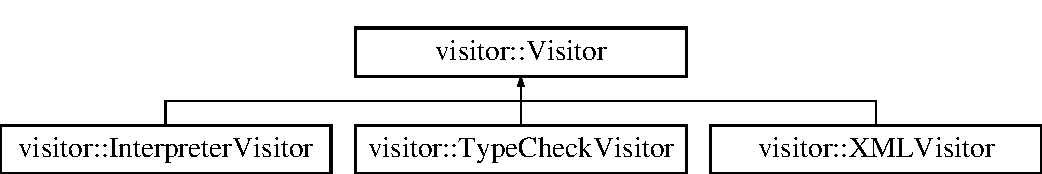
\includegraphics[height=2.000000cm]{df/d8f/classvisitor_1_1Visitor}
\end{center}
\end{figure}
\subsection*{Public Member Functions}
\begin{DoxyCompactItemize}
\item 
\mbox{\Hypertarget{classvisitor_1_1Visitor_a4bcdea24daca965b9b6b286ee92950e6}\label{classvisitor_1_1Visitor_a4bcdea24daca965b9b6b286ee92950e6}} 
virtual void {\bfseries visit} (\hyperlink{classparser_1_1ast_1_1ASTExprNode}{parser\+::ast\+::\+A\+S\+T\+Expr\+Node} $\ast$node)=0
\item 
\mbox{\Hypertarget{classvisitor_1_1Visitor_a46ef198e210079ede5d18a38f41c2470}\label{classvisitor_1_1Visitor_a46ef198e210079ede5d18a38f41c2470}} 
virtual void {\bfseries visit} (\hyperlink{classparser_1_1ast_1_1ASTSimpleExprNode}{parser\+::ast\+::\+A\+S\+T\+Simple\+Expr\+Node} $\ast$node)=0
\item 
\mbox{\Hypertarget{classvisitor_1_1Visitor_a59a4b68c20ef86cdab7bef5a43f4cd93}\label{classvisitor_1_1Visitor_a59a4b68c20ef86cdab7bef5a43f4cd93}} 
virtual void {\bfseries visit} (\hyperlink{classparser_1_1ast_1_1ASTTermNode}{parser\+::ast\+::\+A\+S\+T\+Term\+Node} $\ast$node)=0
\item 
\mbox{\Hypertarget{classvisitor_1_1Visitor_a4f25bb484a62d700a50b8bdbd9be8de1}\label{classvisitor_1_1Visitor_a4f25bb484a62d700a50b8bdbd9be8de1}} 
virtual void {\bfseries visit} (\hyperlink{classparser_1_1ast_1_1ASTLiteralNode}{parser\+::ast\+::\+A\+S\+T\+Literal\+Node}$<$ int $>$ $\ast$node)=0
\item 
\mbox{\Hypertarget{classvisitor_1_1Visitor_a5339173a4229acf5995f0d9291bd318a}\label{classvisitor_1_1Visitor_a5339173a4229acf5995f0d9291bd318a}} 
virtual void {\bfseries visit} (\hyperlink{classparser_1_1ast_1_1ASTLiteralNode}{parser\+::ast\+::\+A\+S\+T\+Literal\+Node}$<$ float $>$ $\ast$node)=0
\item 
\mbox{\Hypertarget{classvisitor_1_1Visitor_a9e0343d14cd0b5e86171270654507df0}\label{classvisitor_1_1Visitor_a9e0343d14cd0b5e86171270654507df0}} 
virtual void {\bfseries visit} (\hyperlink{classparser_1_1ast_1_1ASTLiteralNode}{parser\+::ast\+::\+A\+S\+T\+Literal\+Node}$<$ bool $>$ $\ast$node)=0
\item 
\mbox{\Hypertarget{classvisitor_1_1Visitor_ab94902694cd7e8ac8ff4dfeb462b13be}\label{classvisitor_1_1Visitor_ab94902694cd7e8ac8ff4dfeb462b13be}} 
virtual void {\bfseries visit} (\hyperlink{classparser_1_1ast_1_1ASTLiteralNode}{parser\+::ast\+::\+A\+S\+T\+Literal\+Node}$<$ std\+::string $>$ $\ast$node)=0
\item 
\mbox{\Hypertarget{classvisitor_1_1Visitor_ad22e615f265631f68b499c4d06ae63d4}\label{classvisitor_1_1Visitor_ad22e615f265631f68b499c4d06ae63d4}} 
virtual void {\bfseries visit} (\hyperlink{classparser_1_1ast_1_1ASTFunctionCallNode}{parser\+::ast\+::\+A\+S\+T\+Function\+Call\+Node} $\ast$node)=0
\item 
\mbox{\Hypertarget{classvisitor_1_1Visitor_a5812aac1e9cdcfc8ef582e0a2c2a29d3}\label{classvisitor_1_1Visitor_a5812aac1e9cdcfc8ef582e0a2c2a29d3}} 
virtual void {\bfseries visit} (\hyperlink{classparser_1_1ast_1_1ASTIdentifierNode}{parser\+::ast\+::\+A\+S\+T\+Identifier\+Node} $\ast$node)=0
\item 
\mbox{\Hypertarget{classvisitor_1_1Visitor_a5b6bc3dd238795ca2206605c54c4fdf7}\label{classvisitor_1_1Visitor_a5b6bc3dd238795ca2206605c54c4fdf7}} 
virtual void {\bfseries visit} (\hyperlink{classparser_1_1ast_1_1ASTSubExpression}{parser\+::ast\+::\+A\+S\+T\+Sub\+Expression} $\ast$node)=0
\item 
\mbox{\Hypertarget{classvisitor_1_1Visitor_a7822b18b878fe2d9d788a0a56313f8a7}\label{classvisitor_1_1Visitor_a7822b18b878fe2d9d788a0a56313f8a7}} 
virtual void {\bfseries visit} (\hyperlink{classparser_1_1ast_1_1ASTUnaryNode}{parser\+::ast\+::\+A\+S\+T\+Unary\+Node} $\ast$node)=0
\item 
\mbox{\Hypertarget{classvisitor_1_1Visitor_a4e7e68544d2a28f47d9ff6084bb57e12}\label{classvisitor_1_1Visitor_a4e7e68544d2a28f47d9ff6084bb57e12}} 
virtual void {\bfseries visit} (\hyperlink{classparser_1_1ast_1_1ASTAssignmentNode}{parser\+::ast\+::\+A\+S\+T\+Assignment\+Node} $\ast$node)=0
\item 
\mbox{\Hypertarget{classvisitor_1_1Visitor_ae7a764f5d7b69d3331c8043081d9ad56}\label{classvisitor_1_1Visitor_ae7a764f5d7b69d3331c8043081d9ad56}} 
virtual void {\bfseries visit} (\hyperlink{classparser_1_1ast_1_1ASTVariableDeclStatementNode}{parser\+::ast\+::\+A\+S\+T\+Variable\+Decl\+Statement\+Node} $\ast$node)=0
\item 
\mbox{\Hypertarget{classvisitor_1_1Visitor_addd6d63a62fe049777355144c2f0f0c2}\label{classvisitor_1_1Visitor_addd6d63a62fe049777355144c2f0f0c2}} 
virtual void {\bfseries visit} (\hyperlink{classparser_1_1ast_1_1ASTBlockStatementNode}{parser\+::ast\+::\+A\+S\+T\+Block\+Statement\+Node} $\ast$node)=0
\item 
\mbox{\Hypertarget{classvisitor_1_1Visitor_af26df6fe50b4db86c35469271e91ab63}\label{classvisitor_1_1Visitor_af26df6fe50b4db86c35469271e91ab63}} 
virtual void {\bfseries visit} (\hyperlink{classparser_1_1ast_1_1ASTFunctionDeclStatementNode}{parser\+::ast\+::\+A\+S\+T\+Function\+Decl\+Statement\+Node} $\ast$node)=0
\item 
\mbox{\Hypertarget{classvisitor_1_1Visitor_ad5261c66b0f5e2be160b84238c66d402}\label{classvisitor_1_1Visitor_ad5261c66b0f5e2be160b84238c66d402}} 
virtual void {\bfseries visit} (\hyperlink{classparser_1_1ast_1_1ASTIfStatementNode}{parser\+::ast\+::\+A\+S\+T\+If\+Statement\+Node} $\ast$node)=0
\item 
\mbox{\Hypertarget{classvisitor_1_1Visitor_aab7f6df666a533dc45b1b08b827544a5}\label{classvisitor_1_1Visitor_aab7f6df666a533dc45b1b08b827544a5}} 
virtual void {\bfseries visit} (\hyperlink{classparser_1_1ast_1_1ASTWhileStatementNode}{parser\+::ast\+::\+A\+S\+T\+While\+Statement\+Node} $\ast$node)=0
\item 
\mbox{\Hypertarget{classvisitor_1_1Visitor_a7a60a1a4195ee1d0783c65cd206e8f6f}\label{classvisitor_1_1Visitor_a7a60a1a4195ee1d0783c65cd206e8f6f}} 
virtual void {\bfseries visit} (\hyperlink{classparser_1_1ast_1_1ASTPrintStatementNode}{parser\+::ast\+::\+A\+S\+T\+Print\+Statement\+Node} $\ast$node)=0
\item 
\mbox{\Hypertarget{classvisitor_1_1Visitor_aa25bc7baa436c4ba4817b48b4d4d847c}\label{classvisitor_1_1Visitor_aa25bc7baa436c4ba4817b48b4d4d847c}} 
virtual void {\bfseries visit} (\hyperlink{classparser_1_1ast_1_1ASTReturnStatementNode}{parser\+::ast\+::\+A\+S\+T\+Return\+Statement\+Node} $\ast$node)=0
\item 
\mbox{\Hypertarget{classvisitor_1_1Visitor_a617a1b5872f90a1fcf4a09a1f8ae6999}\label{classvisitor_1_1Visitor_a617a1b5872f90a1fcf4a09a1f8ae6999}} 
virtual void {\bfseries visit} (std\+::vector$<$ std\+::unique\+\_\+ptr$<$ \hyperlink{classparser_1_1ast_1_1ASTNode}{parser\+::ast\+::\+A\+S\+T\+Node} $>$$>$ \&nodes)
\end{DoxyCompactItemize}


The documentation for this class was generated from the following files\+:\begin{DoxyCompactItemize}
\item 
visitor/\hyperlink{Visitor_8h}{Visitor.\+h}\item 
visitor/\hyperlink{Visitor_8cpp}{Visitor.\+cpp}\end{DoxyCompactItemize}

\hypertarget{classvisitor_1_1XMLVisitor}{}\section{visitor\+:\+:X\+M\+L\+Visitor Class Reference}
\label{classvisitor_1_1XMLVisitor}\index{visitor\+::\+X\+M\+L\+Visitor@{visitor\+::\+X\+M\+L\+Visitor}}


{\ttfamily \#include $<$X\+M\+L\+Visitor.\+h$>$}

Inheritance diagram for visitor\+:\+:X\+M\+L\+Visitor\+:\begin{figure}[H]
\begin{center}
\leavevmode
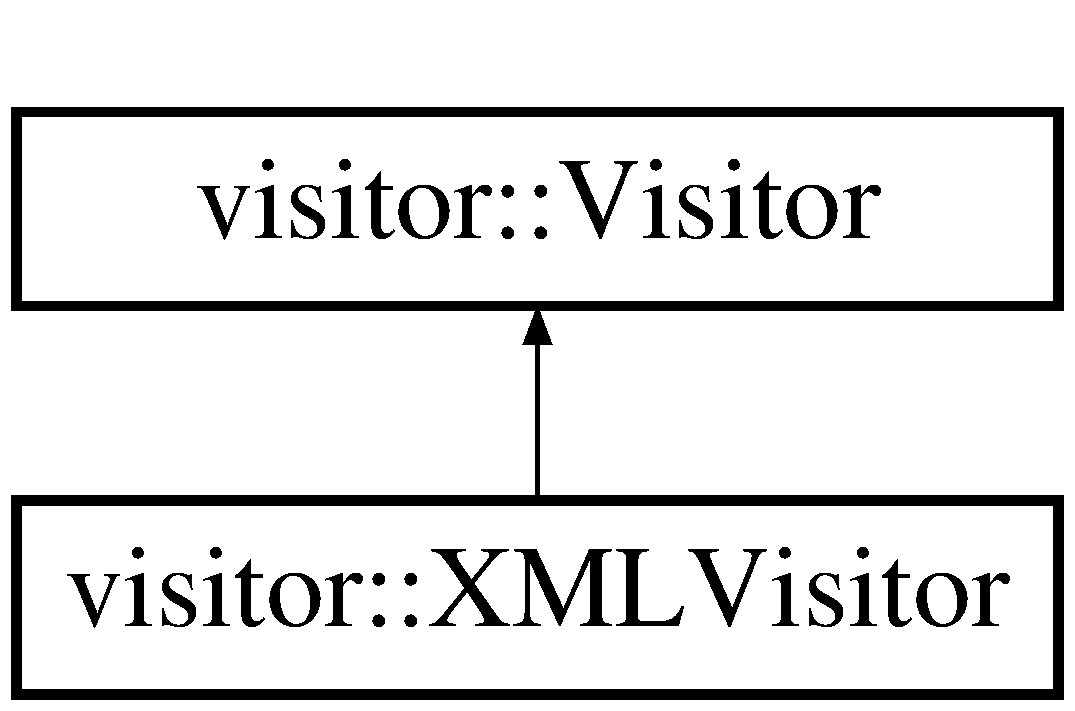
\includegraphics[height=2.000000cm]{d4/de3/classvisitor_1_1XMLVisitor}
\end{center}
\end{figure}
\subsection*{Public Member Functions}
\begin{DoxyCompactItemize}
\item 
\mbox{\Hypertarget{classvisitor_1_1XMLVisitor_ae5c67fecbba47cc79014eac756e831a0}\label{classvisitor_1_1XMLVisitor_ae5c67fecbba47cc79014eac756e831a0}} 
void {\bfseries visit} (\hyperlink{classparser_1_1ast_1_1ASTExprNode}{parser\+::ast\+::\+A\+S\+T\+Expr\+Node} $\ast$node) override
\item 
\mbox{\Hypertarget{classvisitor_1_1XMLVisitor_acbeed8d6d0038f00eee2c7b49ef1a5a0}\label{classvisitor_1_1XMLVisitor_acbeed8d6d0038f00eee2c7b49ef1a5a0}} 
void {\bfseries visit} (\hyperlink{classparser_1_1ast_1_1ASTSimpleExprNode}{parser\+::ast\+::\+A\+S\+T\+Simple\+Expr\+Node} $\ast$node) override
\item 
\mbox{\Hypertarget{classvisitor_1_1XMLVisitor_a64e8855d5fbb07d9e05a6a3d951ce5dd}\label{classvisitor_1_1XMLVisitor_a64e8855d5fbb07d9e05a6a3d951ce5dd}} 
void {\bfseries visit} (\hyperlink{classparser_1_1ast_1_1ASTTermNode}{parser\+::ast\+::\+A\+S\+T\+Term\+Node} $\ast$node) override
\item 
\mbox{\Hypertarget{classvisitor_1_1XMLVisitor_a39da1b61a6fa81efca974ebb17cd5180}\label{classvisitor_1_1XMLVisitor_a39da1b61a6fa81efca974ebb17cd5180}} 
{\footnotesize template$<$typename T $>$ }\\void {\bfseries generic\+Visit} (\hyperlink{classparser_1_1ast_1_1ASTLiteralNode}{parser\+::ast\+::\+A\+S\+T\+Literal\+Node}$<$ T $>$ $\ast$node)
\item 
\mbox{\Hypertarget{classvisitor_1_1XMLVisitor_ad9a170015e08f1e0c89fac6a6218d67c}\label{classvisitor_1_1XMLVisitor_ad9a170015e08f1e0c89fac6a6218d67c}} 
void {\bfseries visit} (\hyperlink{classparser_1_1ast_1_1ASTLiteralNode}{parser\+::ast\+::\+A\+S\+T\+Literal\+Node}$<$ int $>$ $\ast$node) override
\item 
\mbox{\Hypertarget{classvisitor_1_1XMLVisitor_af97fcfa15f3f51b6b655f42e45db2242}\label{classvisitor_1_1XMLVisitor_af97fcfa15f3f51b6b655f42e45db2242}} 
void {\bfseries visit} (\hyperlink{classparser_1_1ast_1_1ASTLiteralNode}{parser\+::ast\+::\+A\+S\+T\+Literal\+Node}$<$ float $>$ $\ast$node) override
\item 
\mbox{\Hypertarget{classvisitor_1_1XMLVisitor_a6bae1cd5475839849045a451518b5faf}\label{classvisitor_1_1XMLVisitor_a6bae1cd5475839849045a451518b5faf}} 
void {\bfseries visit} (\hyperlink{classparser_1_1ast_1_1ASTLiteralNode}{parser\+::ast\+::\+A\+S\+T\+Literal\+Node}$<$ bool $>$ $\ast$node) override
\item 
\mbox{\Hypertarget{classvisitor_1_1XMLVisitor_af024d35bef25b5e69efbfb807b14c01b}\label{classvisitor_1_1XMLVisitor_af024d35bef25b5e69efbfb807b14c01b}} 
void {\bfseries visit} (\hyperlink{classparser_1_1ast_1_1ASTLiteralNode}{parser\+::ast\+::\+A\+S\+T\+Literal\+Node}$<$ std\+::string $>$ $\ast$node) override
\item 
\mbox{\Hypertarget{classvisitor_1_1XMLVisitor_a56bf34a69aa4bf0e9b6092206fdd63bd}\label{classvisitor_1_1XMLVisitor_a56bf34a69aa4bf0e9b6092206fdd63bd}} 
void {\bfseries visit} (\hyperlink{classparser_1_1ast_1_1ASTFunctionCallNode}{parser\+::ast\+::\+A\+S\+T\+Function\+Call\+Node} $\ast$node) override
\item 
\mbox{\Hypertarget{classvisitor_1_1XMLVisitor_aed0c61e7beeebbb525214d5b004e02ad}\label{classvisitor_1_1XMLVisitor_aed0c61e7beeebbb525214d5b004e02ad}} 
void {\bfseries visit} (\hyperlink{classparser_1_1ast_1_1ASTIdentifierNode}{parser\+::ast\+::\+A\+S\+T\+Identifier\+Node} $\ast$node) override
\item 
\mbox{\Hypertarget{classvisitor_1_1XMLVisitor_a28d76153ff33921d6079f2d803d1db33}\label{classvisitor_1_1XMLVisitor_a28d76153ff33921d6079f2d803d1db33}} 
void {\bfseries visit} (\hyperlink{classparser_1_1ast_1_1ASTSubExpression}{parser\+::ast\+::\+A\+S\+T\+Sub\+Expression} $\ast$node) override
\item 
\mbox{\Hypertarget{classvisitor_1_1XMLVisitor_a169ff294dd5f5a51304548cb47f59e98}\label{classvisitor_1_1XMLVisitor_a169ff294dd5f5a51304548cb47f59e98}} 
void {\bfseries visit} (\hyperlink{classparser_1_1ast_1_1ASTUnaryNode}{parser\+::ast\+::\+A\+S\+T\+Unary\+Node} $\ast$node) override
\item 
\mbox{\Hypertarget{classvisitor_1_1XMLVisitor_a126f154abe7bb13ff9cdafb7db1504bf}\label{classvisitor_1_1XMLVisitor_a126f154abe7bb13ff9cdafb7db1504bf}} 
void {\bfseries visit} (\hyperlink{classparser_1_1ast_1_1ASTAssignmentNode}{parser\+::ast\+::\+A\+S\+T\+Assignment\+Node} $\ast$node) override
\item 
\mbox{\Hypertarget{classvisitor_1_1XMLVisitor_abb045f5b98bd4c49efeef96d11fe3700}\label{classvisitor_1_1XMLVisitor_abb045f5b98bd4c49efeef96d11fe3700}} 
void {\bfseries visit} (\hyperlink{classparser_1_1ast_1_1ASTVariableDeclStatementNode}{parser\+::ast\+::\+A\+S\+T\+Variable\+Decl\+Statement\+Node} $\ast$node) override
\item 
\mbox{\Hypertarget{classvisitor_1_1XMLVisitor_a7c5471493a0d87ca94029d1e58945fc3}\label{classvisitor_1_1XMLVisitor_a7c5471493a0d87ca94029d1e58945fc3}} 
void {\bfseries visit} (\hyperlink{classparser_1_1ast_1_1ASTBlockStatementNode}{parser\+::ast\+::\+A\+S\+T\+Block\+Statement\+Node} $\ast$node) override
\item 
\mbox{\Hypertarget{classvisitor_1_1XMLVisitor_ad6625d7bd09f24a294d6a2dc83ed6132}\label{classvisitor_1_1XMLVisitor_ad6625d7bd09f24a294d6a2dc83ed6132}} 
void {\bfseries visit} (\hyperlink{classparser_1_1ast_1_1ASTFunctionDeclStatementNode}{parser\+::ast\+::\+A\+S\+T\+Function\+Decl\+Statement\+Node} $\ast$node) override
\item 
\mbox{\Hypertarget{classvisitor_1_1XMLVisitor_aaa8c7eda00cab075e396171cda5d190b}\label{classvisitor_1_1XMLVisitor_aaa8c7eda00cab075e396171cda5d190b}} 
void {\bfseries visit} (\hyperlink{classparser_1_1ast_1_1ASTIfStatementNode}{parser\+::ast\+::\+A\+S\+T\+If\+Statement\+Node} $\ast$node) override
\item 
\mbox{\Hypertarget{classvisitor_1_1XMLVisitor_aacd004450f9b711b651e6795dea48818}\label{classvisitor_1_1XMLVisitor_aacd004450f9b711b651e6795dea48818}} 
void {\bfseries visit} (\hyperlink{classparser_1_1ast_1_1ASTWhileStatementNode}{parser\+::ast\+::\+A\+S\+T\+While\+Statement\+Node} $\ast$node) override
\item 
\mbox{\Hypertarget{classvisitor_1_1XMLVisitor_a5c2c22238e97f704d5c28bd20918ca78}\label{classvisitor_1_1XMLVisitor_a5c2c22238e97f704d5c28bd20918ca78}} 
void {\bfseries visit} (\hyperlink{classparser_1_1ast_1_1ASTPrintStatementNode}{parser\+::ast\+::\+A\+S\+T\+Print\+Statement\+Node} $\ast$node) override
\item 
\mbox{\Hypertarget{classvisitor_1_1XMLVisitor_aa293c8a26f718d05abaa6bf602d9d49d}\label{classvisitor_1_1XMLVisitor_aa293c8a26f718d05abaa6bf602d9d49d}} 
void {\bfseries visit} (\hyperlink{classparser_1_1ast_1_1ASTReturnStatementNode}{parser\+::ast\+::\+A\+S\+T\+Return\+Statement\+Node} $\ast$node) override
\end{DoxyCompactItemize}


\subsection{Detailed Description}
visit() operators in this class 

The documentation for this class was generated from the following files\+:\begin{DoxyCompactItemize}
\item 
visitor/\hyperlink{XMLVisitor_8h}{X\+M\+L\+Visitor.\+h}\item 
visitor/\hyperlink{XMLVisitor_8cpp}{X\+M\+L\+Visitor.\+cpp}\end{DoxyCompactItemize}

\chapter{File Documentation}
\hypertarget{Exception_8cpp}{}\section{exceptions/\+Exception.cpp File Reference}
\label{Exception_8cpp}\index{exceptions/\+Exception.\+cpp@{exceptions/\+Exception.\+cpp}}
{\ttfamily \#include \char`\"{}Exception.\+h\char`\"{}}\newline


\subsection{Detailed Description}
\begin{DoxyAuthor}{Author}
Mark Said Camilleri 
\end{DoxyAuthor}
\begin{DoxyVersion}{Version}
20170501. 
\end{DoxyVersion}

\hypertarget{Exception_8h}{}\section{exceptions/\+Exception.h File Reference}
\label{Exception_8h}\index{exceptions/\+Exception.\+h@{exceptions/\+Exception.\+h}}
{\ttfamily \#include $<$exception$>$}\newline
{\ttfamily \#include $<$string$>$}\newline
\subsection*{Classes}
\begin{DoxyCompactItemize}
\item 
class \hyperlink{classexceptions_1_1Exception}{exceptions\+::\+Exception}
\end{DoxyCompactItemize}


\subsection{Detailed Description}
\begin{DoxyAuthor}{Author}
Mark Said Camilleri 
\end{DoxyAuthor}
\begin{DoxyVersion}{Version}
20170501. 
\end{DoxyVersion}

\hypertarget{IllegalArgumentException_8cpp}{}\section{exceptions/\+Illegal\+Argument\+Exception.cpp File Reference}
\label{IllegalArgumentException_8cpp}\index{exceptions/\+Illegal\+Argument\+Exception.\+cpp@{exceptions/\+Illegal\+Argument\+Exception.\+cpp}}
{\ttfamily \#include \char`\"{}Illegal\+Argument\+Exception.\+h\char`\"{}}\newline


\subsection{Detailed Description}
\begin{DoxyAuthor}{Author}
Mark Said Camilleri 
\end{DoxyAuthor}
\begin{DoxyVersion}{Version}
20170501. 
\end{DoxyVersion}

\hypertarget{IllegalArgumentException_8h}{}\section{exceptions/\+Illegal\+Argument\+Exception.h File Reference}
\label{IllegalArgumentException_8h}\index{exceptions/\+Illegal\+Argument\+Exception.\+h@{exceptions/\+Illegal\+Argument\+Exception.\+h}}
{\ttfamily \#include \char`\"{}Exception.\+h\char`\"{}}\newline
\subsection*{Classes}
\begin{DoxyCompactItemize}
\item 
class \hyperlink{classexceptions_1_1IllegalArgumentException}{exceptions\+::\+Illegal\+Argument\+Exception}
\end{DoxyCompactItemize}


\subsection{Detailed Description}
\begin{DoxyAuthor}{Author}
Mark Said Camilleri 
\end{DoxyAuthor}
\begin{DoxyVersion}{Version}
20170501. 
\end{DoxyVersion}

\hypertarget{SyntaxError_8h}{}\section{exceptions/\+Syntax\+Error.h File Reference}
\label{SyntaxError_8h}\index{exceptions/\+Syntax\+Error.\+h@{exceptions/\+Syntax\+Error.\+h}}
{\ttfamily \#include \char`\"{}Exception.\+h\char`\"{}}\newline
\subsection*{Classes}
\begin{DoxyCompactItemize}
\item 
class \hyperlink{classexceptions_1_1SyntaxError}{exceptions\+::\+Syntax\+Error}
\end{DoxyCompactItemize}


\subsection{Detailed Description}
\begin{DoxyAuthor}{Author}
Mark Said Camilleri 
\end{DoxyAuthor}
\begin{DoxyVersion}{Version}
20170426 
\end{DoxyVersion}

\hypertarget{TypeError_8cpp}{}\section{exceptions/\+Type\+Error.cpp File Reference}
\label{TypeError_8cpp}\index{exceptions/\+Type\+Error.\+cpp@{exceptions/\+Type\+Error.\+cpp}}
{\ttfamily \#include \char`\"{}Type\+Error.\+h\char`\"{}}\newline


\subsection{Detailed Description}
\begin{DoxyAuthor}{Author}
Mark Said Camilleri 
\end{DoxyAuthor}
\begin{DoxyVersion}{Version}
20170519. 
\end{DoxyVersion}

\hypertarget{TypeError_8h}{}\section{exceptions/\+Type\+Error.h File Reference}
\label{TypeError_8h}\index{exceptions/\+Type\+Error.\+h@{exceptions/\+Type\+Error.\+h}}
{\ttfamily \#include \char`\"{}Exception.\+h\char`\"{}}\newline
\subsection*{Classes}
\begin{DoxyCompactItemize}
\item 
class \hyperlink{classexceptions_1_1TypeError}{exceptions\+::\+Type\+Error}
\end{DoxyCompactItemize}


\subsection{Detailed Description}
\begin{DoxyAuthor}{Author}
Mark Said Camilleri 
\end{DoxyAuthor}
\begin{DoxyVersion}{Version}
20170519. 
\end{DoxyVersion}

\hypertarget{Lexer_8h}{}\section{lexer/\+Lexer.h File Reference}
\label{Lexer_8h}\index{lexer/\+Lexer.\+h@{lexer/\+Lexer.\+h}}
{\ttfamily \#include $<$array$>$}\newline
{\ttfamily \#include $<$vector$>$}\newline
{\ttfamily \#include $<$functional$>$}\newline
{\ttfamily \#include $<$unordered\+\_\+set$>$}\newline
{\ttfamily \#include $<$unordered\+\_\+map$>$}\newline
{\ttfamily \#include \char`\"{}Token\+Type.\+h\char`\"{}}\newline
\subsection*{Classes}
\begin{DoxyCompactItemize}
\item 
struct \hyperlink{structlexer_1_1Position}{lexer\+::\+Position}
\item 
class \hyperlink{classlexer_1_1Lexer}{lexer\+::\+Lexer}
\end{DoxyCompactItemize}
\subsection*{Macros}
\begin{DoxyCompactItemize}
\item 
\mbox{\Hypertarget{Lexer_8h_a735563036dced0b7d6cc98f97ea4978b}\label{Lexer_8h_a735563036dced0b7d6cc98f97ea4978b}} 
\#define {\bfseries E\+RR}~-\/99
\item 
\mbox{\Hypertarget{Lexer_8h_a6572f1706059832f94025fa12c6c45ed}\label{Lexer_8h_a6572f1706059832f94025fa12c6c45ed}} 
\#define {\bfseries A\+L\+P\+H\+A\+B\+E\+T\+\_\+\+S\+I\+ZE}~17
\item 
\mbox{\Hypertarget{Lexer_8h_a7c84ffa503c19944f71692dfcb1dfda5}\label{Lexer_8h_a7c84ffa503c19944f71692dfcb1dfda5}} 
\#define {\bfseries N\+O\+\_\+\+O\+F\+\_\+\+S\+T\+A\+T\+ES}~22 /$\ast$ 0 -\/ 21 $\ast$/
\item 
\mbox{\Hypertarget{Lexer_8h_a61be4a4e1aee2cef4f2fcb2313ae6389}\label{Lexer_8h_a61be4a4e1aee2cef4f2fcb2313ae6389}} 
\#define {\bfseries T\+E\+R\+M\+I\+N\+A\+L\+\_\+\+N\+O\+DE}~\{E\+RR, E\+RR, E\+RR, E\+RR, E\+RR, E\+RR, E\+RR, E\+RR, E\+RR, E\+RR, E\+RR, E\+RR, E\+RR, E\+RR, E\+RR, E\+RR, E\+RR\}
\end{DoxyCompactItemize}
\subsection*{Typedefs}
\begin{DoxyCompactItemize}
\item 
typedef struct \hyperlink{structlexer_1_1Position}{lexer\+::\+Position} \hyperlink{Lexer_8h_ad8afe18e2b9a97e1721eff7ca1d5360b}{lexer\+::\+Position}
\end{DoxyCompactItemize}


\subsection{Detailed Description}
\begin{DoxyAuthor}{Author}
Mark Said Camilleri 
\end{DoxyAuthor}
\begin{DoxyVersion}{Version}
20170426 
\end{DoxyVersion}


\subsection{Typedef Documentation}
\mbox{\Hypertarget{Lexer_8h_file_ad8afe18e2b9a97e1721eff7ca1d5360b}\label{Lexer_8h_file_ad8afe18e2b9a97e1721eff7ca1d5360b}} 
\index{Lexer.\+h@{Lexer.\+h}!Position@{Position}}
\index{Position@{Position}!Lexer.\+h@{Lexer.\+h}}
\subsubsection{\texorpdfstring{Position}{Position}}
{\footnotesize\ttfamily typedef struct \hyperlink{structlexer_1_1Position}{lexer\+::\+Position}  \hyperlink{structlexer_1_1Position}{lexer\+::\+Position}}

This struct represents the cursor used to read the file input 
\hypertarget{TokenType_8h}{}\section{lexer/\+Token\+Type.h File Reference}
\label{TokenType_8h}\index{lexer/\+Token\+Type.\+h@{lexer/\+Token\+Type.\+h}}
{\ttfamily \#include $<$string$>$}\newline
\subsection*{Classes}
\begin{DoxyCompactItemize}
\item 
class \hyperlink{classlexer_1_1Token}{lexer\+::\+Token}
\end{DoxyCompactItemize}
\subsection*{Enumerations}
\begin{DoxyCompactItemize}
\item 
\mbox{\Hypertarget{TokenType_8h_a8609501a650c2bf52e8397c88de5770f}\label{TokenType_8h_a8609501a650c2bf52e8397c88de5770f}} 
enum \hyperlink{TokenType_8h_a8609501a650c2bf52e8397c88de5770f}{lexer\+::\+Token\+Type} \{ \newline
{\bfseries T\+O\+K\+\_\+\+I\+D\+E\+N\+T\+I\+F\+I\+ER}, 
{\bfseries T\+O\+K\+\_\+\+I\+N\+T\+E\+G\+E\+R\+\_\+\+L\+I\+T\+E\+R\+AL}, 
{\bfseries T\+O\+K\+\_\+\+R\+E\+A\+L\+\_\+\+L\+I\+T\+E\+R\+AL}, 
{\bfseries T\+O\+K\+\_\+\+B\+O\+O\+L\+\_\+\+L\+I\+T\+E\+R\+AL}, 
\newline
{\bfseries T\+O\+K\+\_\+\+S\+T\+R\+I\+N\+G\+\_\+\+L\+I\+T\+E\+R\+AL}, 
{\bfseries T\+O\+K\+\_\+\+A\+D\+D\+I\+T\+I\+ON}, 
{\bfseries T\+O\+K\+\_\+\+S\+U\+B\+T\+R\+A\+C\+T\+I\+ON}, 
{\bfseries T\+O\+K\+\_\+\+M\+U\+L\+T\+I\+P\+L\+I\+C\+A\+T\+I\+ON}, 
\newline
{\bfseries T\+O\+K\+\_\+\+D\+I\+V\+I\+S\+I\+ON}, 
{\bfseries T\+O\+K\+\_\+\+R\+E\+L\+A\+T\+I\+O\+N\+A\+L\+\_\+\+OP}, 
{\bfseries T\+O\+K\+\_\+\+A\+S\+S\+I\+G\+N\+M\+E\+N\+T\+\_\+\+E\+Q\+U\+A\+LS}, 
{\bfseries T\+O\+K\+\_\+\+S\+I\+N\+G\+L\+E\+\_\+\+L\+I\+N\+E\+\_\+\+C\+O\+M\+M\+E\+NT}, 
\newline
{\bfseries T\+O\+K\+\_\+\+M\+U\+L\+T\+I\+\_\+\+L\+I\+N\+E\+\_\+\+C\+O\+M\+M\+E\+NT}, 
{\bfseries T\+O\+K\+\_\+\+P\+U\+N\+C\+T\+U\+A\+T\+I\+ON}, 
{\bfseries T\+O\+K\+\_\+\+A\+ND}, 
{\bfseries T\+O\+K\+\_\+\+OR}, 
\newline
{\bfseries T\+O\+K\+\_\+\+N\+OT}, 
{\bfseries T\+O\+K\+\_\+\+IF}, 
{\bfseries T\+O\+K\+\_\+\+E\+L\+SE}, 
{\bfseries T\+O\+K\+\_\+\+W\+H\+I\+LE}, 
\newline
{\bfseries T\+O\+K\+\_\+\+T\+Y\+PE}, 
{\bfseries T\+O\+K\+\_\+\+S\+ET}, 
{\bfseries T\+O\+K\+\_\+\+V\+AR}, 
{\bfseries T\+O\+K\+\_\+\+P\+R\+I\+NT}, 
\newline
{\bfseries T\+O\+K\+\_\+\+D\+EF}, 
{\bfseries T\+O\+K\+\_\+\+R\+E\+T\+U\+RN}, 
{\bfseries T\+O\+K\+\_\+\+E\+OF}
 \}\begin{DoxyCompactList}\small\item\em The possible tokens that can be returned by the lexer. \end{DoxyCompactList}
\end{DoxyCompactItemize}


\subsection{Detailed Description}
\begin{DoxyAuthor}{Author}
Mark Said Camilleri 
\end{DoxyAuthor}
\begin{DoxyVersion}{Version}
20170426 
\end{DoxyVersion}

\hypertarget{ASTExprNode_8h}{}\section{parser/ast/\+A\+S\+T\+Expr\+Node.h File Reference}
\label{ASTExprNode_8h}\index{parser/ast/\+A\+S\+T\+Expr\+Node.\+h@{parser/ast/\+A\+S\+T\+Expr\+Node.\+h}}
{\ttfamily \#include $<$memory$>$}\newline
{\ttfamily \#include \char`\"{}A\+S\+T\+Node.\+h\char`\"{}}\newline
{\ttfamily \#include \char`\"{}expression/\+A\+S\+T\+Simple\+Expr\+Node.\+h\char`\"{}}\newline
\subsection*{Classes}
\begin{DoxyCompactItemize}
\item 
class \hyperlink{classparser_1_1ast_1_1ASTExprNode}{parser\+::ast\+::\+A\+S\+T\+Expr\+Node}
\end{DoxyCompactItemize}
\subsection*{Enumerations}
\begin{DoxyCompactItemize}
\item 
enum \hyperlink{ASTExprNode_8h_ade5793e91a548ec55c1a8e776984297a}{parser\+::ast\+::\+Rel\+Op\+Type} \{ \newline
\hyperlink{ASTExprNode_8h_ade5793e91a548ec55c1a8e776984297aac882da559ca838834523a65f96c3ba7f}{parser\+::ast\+::\+R\+E\+L\+\_\+\+G\+R\+E\+A\+T\+ER}, 
\hyperlink{ASTExprNode_8h_ade5793e91a548ec55c1a8e776984297aada062d3cd0b06a82b67bf9a9dba10c65}{parser\+::ast\+::\+R\+E\+L\+\_\+\+G\+R\+E\+A\+T\+E\+R\+\_\+\+O\+R\+\_\+\+E\+Q\+U\+A\+LS}, 
\hyperlink{ASTExprNode_8h_ade5793e91a548ec55c1a8e776984297aaae06cc6dc61ec0c42aa23e8d13a0759f}{parser\+::ast\+::\+R\+E\+L\+\_\+\+E\+Q\+U\+A\+LS}, 
\hyperlink{ASTExprNode_8h_ade5793e91a548ec55c1a8e776984297aa11450272997b012463a75eee1c76200f}{parser\+::ast\+::\+R\+E\+L\+\_\+\+N\+O\+T\+\_\+\+E\+Q\+U\+A\+LS}, 
\newline
\hyperlink{ASTExprNode_8h_ade5793e91a548ec55c1a8e776984297aa0a907adaea5764c8faa4a8f9b0b72825}{parser\+::ast\+::\+R\+E\+L\+\_\+\+L\+E\+S\+S\+\_\+\+O\+R\+\_\+\+E\+Q\+U\+A\+LS}, 
\hyperlink{ASTExprNode_8h_ade5793e91a548ec55c1a8e776984297aac20237403a2ff54686fa3a5925451b64}{parser\+::ast\+::\+R\+E\+L\+\_\+\+L\+E\+SS}
 \}\begin{DoxyCompactList}\small\item\em Enumerated type representing relational operators that can be used for an expression. \end{DoxyCompactList}
\end{DoxyCompactItemize}


\subsection{Detailed Description}
\begin{DoxyAuthor}{Author}
Mark Said Camilleri 
\end{DoxyAuthor}
\begin{DoxyVersion}{Version}
20170430 
\end{DoxyVersion}


\subsection{Enumeration Type Documentation}
\mbox{\Hypertarget{ASTExprNode_8h_file_ade5793e91a548ec55c1a8e776984297a}\label{ASTExprNode_8h_file_ade5793e91a548ec55c1a8e776984297a}} 
\index{A\+S\+T\+Expr\+Node.\+h@{A\+S\+T\+Expr\+Node.\+h}!Rel\+Op\+Type@{Rel\+Op\+Type}}
\index{Rel\+Op\+Type@{Rel\+Op\+Type}!A\+S\+T\+Expr\+Node.\+h@{A\+S\+T\+Expr\+Node.\+h}}
\subsubsection{\texorpdfstring{Rel\+Op\+Type}{RelOpType}}
{\footnotesize\ttfamily enum \hyperlink{ASTExprNode_8h_ade5793e91a548ec55c1a8e776984297a}{parser\+::ast\+::\+Rel\+Op\+Type}}



Enumerated type representing relational operators that can be used for an expression. 

\begin{DoxyEnumFields}{Enumerator}
\raisebox{\heightof{T}}[0pt][0pt]{\index{R\+E\+L\+\_\+\+G\+R\+E\+A\+T\+ER@{R\+E\+L\+\_\+\+G\+R\+E\+A\+T\+ER}!A\+S\+T\+Expr\+Node.\+h@{A\+S\+T\+Expr\+Node.\+h}}\index{A\+S\+T\+Expr\+Node.\+h@{A\+S\+T\+Expr\+Node.\+h}!R\+E\+L\+\_\+\+G\+R\+E\+A\+T\+ER@{R\+E\+L\+\_\+\+G\+R\+E\+A\+T\+ER}}}\mbox{\Hypertarget{ASTExprNode_8h_ade5793e91a548ec55c1a8e776984297aac882da559ca838834523a65f96c3ba7f}\label{ASTExprNode_8h_ade5793e91a548ec55c1a8e776984297aac882da559ca838834523a65f96c3ba7f}} 
R\+E\+L\+\_\+\+G\+R\+E\+A\+T\+ER&Greater than ({\ttfamily $>$}) operator. \\
\hline

\raisebox{\heightof{T}}[0pt][0pt]{\index{R\+E\+L\+\_\+\+G\+R\+E\+A\+T\+E\+R\+\_\+\+O\+R\+\_\+\+E\+Q\+U\+A\+LS@{R\+E\+L\+\_\+\+G\+R\+E\+A\+T\+E\+R\+\_\+\+O\+R\+\_\+\+E\+Q\+U\+A\+LS}!A\+S\+T\+Expr\+Node.\+h@{A\+S\+T\+Expr\+Node.\+h}}\index{A\+S\+T\+Expr\+Node.\+h@{A\+S\+T\+Expr\+Node.\+h}!R\+E\+L\+\_\+\+G\+R\+E\+A\+T\+E\+R\+\_\+\+O\+R\+\_\+\+E\+Q\+U\+A\+LS@{R\+E\+L\+\_\+\+G\+R\+E\+A\+T\+E\+R\+\_\+\+O\+R\+\_\+\+E\+Q\+U\+A\+LS}}}\mbox{\Hypertarget{ASTExprNode_8h_ade5793e91a548ec55c1a8e776984297aada062d3cd0b06a82b67bf9a9dba10c65}\label{ASTExprNode_8h_ade5793e91a548ec55c1a8e776984297aada062d3cd0b06a82b67bf9a9dba10c65}} 
R\+E\+L\+\_\+\+G\+R\+E\+A\+T\+E\+R\+\_\+\+O\+R\+\_\+\+E\+Q\+U\+A\+LS&Greater than or equals ({\ttfamily $>$=}) operator. \\
\hline

\raisebox{\heightof{T}}[0pt][0pt]{\index{R\+E\+L\+\_\+\+E\+Q\+U\+A\+LS@{R\+E\+L\+\_\+\+E\+Q\+U\+A\+LS}!A\+S\+T\+Expr\+Node.\+h@{A\+S\+T\+Expr\+Node.\+h}}\index{A\+S\+T\+Expr\+Node.\+h@{A\+S\+T\+Expr\+Node.\+h}!R\+E\+L\+\_\+\+E\+Q\+U\+A\+LS@{R\+E\+L\+\_\+\+E\+Q\+U\+A\+LS}}}\mbox{\Hypertarget{ASTExprNode_8h_ade5793e91a548ec55c1a8e776984297aaae06cc6dc61ec0c42aa23e8d13a0759f}\label{ASTExprNode_8h_ade5793e91a548ec55c1a8e776984297aaae06cc6dc61ec0c42aa23e8d13a0759f}} 
R\+E\+L\+\_\+\+E\+Q\+U\+A\+LS&Equals ({\ttfamily ==}) operator. \\
\hline

\raisebox{\heightof{T}}[0pt][0pt]{\index{R\+E\+L\+\_\+\+N\+O\+T\+\_\+\+E\+Q\+U\+A\+LS@{R\+E\+L\+\_\+\+N\+O\+T\+\_\+\+E\+Q\+U\+A\+LS}!A\+S\+T\+Expr\+Node.\+h@{A\+S\+T\+Expr\+Node.\+h}}\index{A\+S\+T\+Expr\+Node.\+h@{A\+S\+T\+Expr\+Node.\+h}!R\+E\+L\+\_\+\+N\+O\+T\+\_\+\+E\+Q\+U\+A\+LS@{R\+E\+L\+\_\+\+N\+O\+T\+\_\+\+E\+Q\+U\+A\+LS}}}\mbox{\Hypertarget{ASTExprNode_8h_ade5793e91a548ec55c1a8e776984297aa11450272997b012463a75eee1c76200f}\label{ASTExprNode_8h_ade5793e91a548ec55c1a8e776984297aa11450272997b012463a75eee1c76200f}} 
R\+E\+L\+\_\+\+N\+O\+T\+\_\+\+E\+Q\+U\+A\+LS&Not Equals ({\ttfamily !=}) operator. \\
\hline

\raisebox{\heightof{T}}[0pt][0pt]{\index{R\+E\+L\+\_\+\+L\+E\+S\+S\+\_\+\+O\+R\+\_\+\+E\+Q\+U\+A\+LS@{R\+E\+L\+\_\+\+L\+E\+S\+S\+\_\+\+O\+R\+\_\+\+E\+Q\+U\+A\+LS}!A\+S\+T\+Expr\+Node.\+h@{A\+S\+T\+Expr\+Node.\+h}}\index{A\+S\+T\+Expr\+Node.\+h@{A\+S\+T\+Expr\+Node.\+h}!R\+E\+L\+\_\+\+L\+E\+S\+S\+\_\+\+O\+R\+\_\+\+E\+Q\+U\+A\+LS@{R\+E\+L\+\_\+\+L\+E\+S\+S\+\_\+\+O\+R\+\_\+\+E\+Q\+U\+A\+LS}}}\mbox{\Hypertarget{ASTExprNode_8h_ade5793e91a548ec55c1a8e776984297aa0a907adaea5764c8faa4a8f9b0b72825}\label{ASTExprNode_8h_ade5793e91a548ec55c1a8e776984297aa0a907adaea5764c8faa4a8f9b0b72825}} 
R\+E\+L\+\_\+\+L\+E\+S\+S\+\_\+\+O\+R\+\_\+\+E\+Q\+U\+A\+LS&Less than or equals ({\ttfamily $<$=}) operator. \\
\hline

\raisebox{\heightof{T}}[0pt][0pt]{\index{R\+E\+L\+\_\+\+L\+E\+SS@{R\+E\+L\+\_\+\+L\+E\+SS}!A\+S\+T\+Expr\+Node.\+h@{A\+S\+T\+Expr\+Node.\+h}}\index{A\+S\+T\+Expr\+Node.\+h@{A\+S\+T\+Expr\+Node.\+h}!R\+E\+L\+\_\+\+L\+E\+SS@{R\+E\+L\+\_\+\+L\+E\+SS}}}\mbox{\Hypertarget{ASTExprNode_8h_ade5793e91a548ec55c1a8e776984297aac20237403a2ff54686fa3a5925451b64}\label{ASTExprNode_8h_ade5793e91a548ec55c1a8e776984297aac20237403a2ff54686fa3a5925451b64}} 
R\+E\+L\+\_\+\+L\+E\+SS&Less than ({\ttfamily $<$} operator) \\
\hline

\end{DoxyEnumFields}

\hypertarget{ASTFactorNode_8h}{}\section{parser/ast/expression/\+A\+S\+T\+Factor\+Node.h File Reference}
\label{ASTFactorNode_8h}\index{parser/ast/expression/\+A\+S\+T\+Factor\+Node.\+h@{parser/ast/expression/\+A\+S\+T\+Factor\+Node.\+h}}
{\ttfamily \#include \char`\"{}../\+A\+S\+T\+Node.\+h\char`\"{}}\newline
\subsection*{Classes}
\begin{DoxyCompactItemize}
\item 
class \hyperlink{classparser_1_1ast_1_1ASTFactorNode}{parser\+::ast\+::\+A\+S\+T\+Factor\+Node}
\end{DoxyCompactItemize}
\subsection*{Enumerations}
\begin{DoxyCompactItemize}
\item 
enum \hyperlink{ASTFactorNode_8h_afbe2fcc03ef15b74a0c1ed1cda7ab0e8}{parser\+::ast\+::\+Factor\+Type} \{ \newline
{\bfseries L\+I\+T\+E\+R\+AL}, 
{\bfseries I\+D\+E\+N\+T\+I\+F\+I\+ER}, 
{\bfseries F\+U\+N\+C\+T\+I\+O\+N\+\_\+\+C\+A\+LL}, 
{\bfseries S\+U\+B\+\_\+\+E\+X\+P\+R\+E\+S\+S\+I\+ON}, 
\newline
{\bfseries U\+N\+A\+RY}
 \}
\end{DoxyCompactItemize}


\subsection{Detailed Description}
\begin{DoxyAuthor}{Author}
Mark Said Camilleri 
\end{DoxyAuthor}
\begin{DoxyVersion}{Version}
20170503. 
\end{DoxyVersion}


\subsection{Enumeration Type Documentation}
\mbox{\Hypertarget{ASTFactorNode_8h_file_afbe2fcc03ef15b74a0c1ed1cda7ab0e8}\label{ASTFactorNode_8h_file_afbe2fcc03ef15b74a0c1ed1cda7ab0e8}} 
\index{A\+S\+T\+Factor\+Node.\+h@{A\+S\+T\+Factor\+Node.\+h}!Factor\+Type@{Factor\+Type}}
\index{Factor\+Type@{Factor\+Type}!A\+S\+T\+Factor\+Node.\+h@{A\+S\+T\+Factor\+Node.\+h}}
\subsubsection{\texorpdfstring{Factor\+Type}{FactorType}}
{\footnotesize\ttfamily enum \hyperlink{ASTFactorNode_8h_afbe2fcc03ef15b74a0c1ed1cda7ab0e8}{parser\+::ast\+::\+Factor\+Type}}

Strongly typed factor type 
\hypertarget{ASTTermNode_8h}{}\section{parser/ast/expression/\+A\+S\+T\+Term\+Node.h File Reference}
\label{ASTTermNode_8h}\index{parser/ast/expression/\+A\+S\+T\+Term\+Node.\+h@{parser/ast/expression/\+A\+S\+T\+Term\+Node.\+h}}
{\ttfamily \#include $<$memory$>$}\newline
{\ttfamily \#include \char`\"{}A\+S\+T\+Factor\+Node.\+h\char`\"{}}\newline
{\ttfamily \#include \char`\"{}../\+A\+S\+T\+Node.\+h\char`\"{}}\newline
\subsection*{Classes}
\begin{DoxyCompactItemize}
\item 
class \hyperlink{classparser_1_1ast_1_1ASTTermNode}{parser\+::ast\+::\+A\+S\+T\+Term\+Node}
\end{DoxyCompactItemize}
\subsection*{Enumerations}
\begin{DoxyCompactItemize}
\item 
enum \hyperlink{ASTTermNode_8h_a56419c32f44e139982c327d8375a27a7}{parser\+::ast\+::\+Multiplicative\+Op} \{ {\bfseries M\+U\+L\+T\+I\+P\+L\+I\+C\+A\+T\+I\+ON}, 
{\bfseries D\+I\+V\+I\+S\+I\+ON}, 
{\bfseries A\+ND}
 \}
\end{DoxyCompactItemize}


\subsection{Detailed Description}
\begin{DoxyAuthor}{Author}
Mark Said Camilleri 
\end{DoxyAuthor}
\begin{DoxyVersion}{Version}
20170503 
\end{DoxyVersion}


\subsection{Enumeration Type Documentation}
\mbox{\Hypertarget{ASTTermNode_8h_file_a56419c32f44e139982c327d8375a27a7}\label{ASTTermNode_8h_file_a56419c32f44e139982c327d8375a27a7}} 
\index{A\+S\+T\+Term\+Node.\+h@{A\+S\+T\+Term\+Node.\+h}!Multiplicative\+Op@{Multiplicative\+Op}}
\index{Multiplicative\+Op@{Multiplicative\+Op}!A\+S\+T\+Term\+Node.\+h@{A\+S\+T\+Term\+Node.\+h}}
\subsubsection{\texorpdfstring{Multiplicative\+Op}{MultiplicativeOp}}
{\footnotesize\ttfamily enum \hyperlink{ASTTermNode_8h_a56419c32f44e139982c327d8375a27a7}{parser\+::ast\+::\+Multiplicative\+Op}}

Strong type for the multiplicative operator 
\hypertarget{ASTFunctionCallNode_8cpp}{}\section{parser/ast/expression/factor/\+A\+S\+T\+Function\+Call\+Node.cpp File Reference}
\label{ASTFunctionCallNode_8cpp}\index{parser/ast/expression/factor/\+A\+S\+T\+Function\+Call\+Node.\+cpp@{parser/ast/expression/factor/\+A\+S\+T\+Function\+Call\+Node.\+cpp}}
{\ttfamily \#include $<$iostream$>$}\newline
{\ttfamily \#include \char`\"{}A\+S\+T\+Function\+Call\+Node.\+h\char`\"{}}\newline
{\ttfamily \#include \char`\"{}../../../../visitor/\+Visitor.\+h\char`\"{}}\newline


\subsection{Detailed Description}
\begin{DoxyAuthor}{Author}
Mark Said Camilleri 
\end{DoxyAuthor}
\begin{DoxyVersion}{Version}
20170503. 
\end{DoxyVersion}

\hypertarget{ASTFunctionCallNode_8h}{}\section{parser/ast/expression/factor/\+A\+S\+T\+Function\+Call\+Node.h File Reference}
\label{ASTFunctionCallNode_8h}\index{parser/ast/expression/factor/\+A\+S\+T\+Function\+Call\+Node.\+h@{parser/ast/expression/factor/\+A\+S\+T\+Function\+Call\+Node.\+h}}
{\ttfamily \#include $<$vector$>$}\newline
{\ttfamily \#include \char`\"{}../\+A\+S\+T\+Factor\+Node.\+h\char`\"{}}\newline
{\ttfamily \#include \char`\"{}A\+S\+T\+Identifier\+Node.\+h\char`\"{}}\newline
{\ttfamily \#include \char`\"{}../../\+A\+S\+T\+Expr\+Node.\+h\char`\"{}}\newline
\subsection*{Classes}
\begin{DoxyCompactItemize}
\item 
class \hyperlink{classparser_1_1ast_1_1ASTFunctionCallNode}{parser\+::ast\+::\+A\+S\+T\+Function\+Call\+Node}
\end{DoxyCompactItemize}


\subsection{Detailed Description}
\begin{DoxyAuthor}{Author}
Mark Said Camilleri 
\end{DoxyAuthor}
\begin{DoxyVersion}{Version}
20170503. 
\end{DoxyVersion}

\hypertarget{ASTIdentifierNode_8cpp}{}\section{parser/ast/expression/factor/\+A\+S\+T\+Identifier\+Node.cpp File Reference}
\label{ASTIdentifierNode_8cpp}\index{parser/ast/expression/factor/\+A\+S\+T\+Identifier\+Node.\+cpp@{parser/ast/expression/factor/\+A\+S\+T\+Identifier\+Node.\+cpp}}
{\ttfamily \#include $<$iostream$>$}\newline
{\ttfamily \#include \char`\"{}A\+S\+T\+Identifier\+Node.\+h\char`\"{}}\newline
{\ttfamily \#include \char`\"{}../../../../visitor/\+Visitor.\+h\char`\"{}}\newline


\subsection{Detailed Description}
\begin{DoxyAuthor}{Author}
Mark Said Camilleri 
\end{DoxyAuthor}
\begin{DoxyVersion}{Version}
20170503. 
\end{DoxyVersion}

\hypertarget{ASTIdentifierNode_8h}{}\section{parser/ast/expression/factor/\+A\+S\+T\+Identifier\+Node.h File Reference}
\label{ASTIdentifierNode_8h}\index{parser/ast/expression/factor/\+A\+S\+T\+Identifier\+Node.\+h@{parser/ast/expression/factor/\+A\+S\+T\+Identifier\+Node.\+h}}
{\ttfamily \#include $<$string$>$}\newline
{\ttfamily \#include $<$memory$>$}\newline
{\ttfamily \#include \char`\"{}../\+A\+S\+T\+Factor\+Node.\+h\char`\"{}}\newline
{\ttfamily \#include \char`\"{}../../\+A\+S\+T\+Node.\+h\char`\"{}}\newline
\subsection*{Classes}
\begin{DoxyCompactItemize}
\item 
class \hyperlink{classparser_1_1ast_1_1ASTIdentifierNode}{parser\+::ast\+::\+A\+S\+T\+Identifier\+Node}
\end{DoxyCompactItemize}


\subsection{Detailed Description}
\begin{DoxyAuthor}{Author}
Mark Said Camilleri 
\end{DoxyAuthor}
\begin{DoxyVersion}{Version}
20170503. 
\end{DoxyVersion}

\hypertarget{ASTLiteralNode_8cpp}{}\section{parser/ast/expression/factor/\+A\+S\+T\+Literal\+Node.cpp File Reference}
\label{ASTLiteralNode_8cpp}\index{parser/ast/expression/factor/\+A\+S\+T\+Literal\+Node.\+cpp@{parser/ast/expression/factor/\+A\+S\+T\+Literal\+Node.\+cpp}}
{\ttfamily \#include \char`\"{}A\+S\+T\+Literal\+Node.\+h\char`\"{}}\newline
{\ttfamily \#include \char`\"{}../../../../visitor/\+Visitor.\+h\char`\"{}}\newline


\subsection{Detailed Description}
\begin{DoxyAuthor}{Author}
Mark Said Camilleri 
\end{DoxyAuthor}
\begin{DoxyVersion}{Version}
20170503. 
\end{DoxyVersion}

\hypertarget{ASTLiteralNode_8h}{}\section{parser/ast/expression/factor/\+A\+S\+T\+Literal\+Node.h File Reference}
\label{ASTLiteralNode_8h}\index{parser/ast/expression/factor/\+A\+S\+T\+Literal\+Node.\+h@{parser/ast/expression/factor/\+A\+S\+T\+Literal\+Node.\+h}}
{\ttfamily \#include $<$string$>$}\newline
{\ttfamily \#include \char`\"{}../\+A\+S\+T\+Factor\+Node.\+h\char`\"{}}\newline
{\ttfamily \#include \char`\"{}../../\+A\+S\+T\+Node.\+h\char`\"{}}\newline
\subsection*{Classes}
\begin{DoxyCompactItemize}
\item 
class \hyperlink{classparser_1_1ast_1_1ASTLiteralNode}{parser\+::ast\+::\+A\+S\+T\+Literal\+Node$<$ T $>$}
\end{DoxyCompactItemize}


\subsection{Detailed Description}
\begin{DoxyAuthor}{Author}
Mark Said Camilleri 
\end{DoxyAuthor}
\begin{DoxyVersion}{Version}
20170503. 
\end{DoxyVersion}

\hypertarget{ASTSubExpression_8cpp}{}\section{parser/ast/expression/factor/\+A\+S\+T\+Sub\+Expression.cpp File Reference}
\label{ASTSubExpression_8cpp}\index{parser/ast/expression/factor/\+A\+S\+T\+Sub\+Expression.\+cpp@{parser/ast/expression/factor/\+A\+S\+T\+Sub\+Expression.\+cpp}}
{\ttfamily \#include \char`\"{}A\+S\+T\+Sub\+Expression.\+h\char`\"{}}\newline
{\ttfamily \#include \char`\"{}../../../../visitor/\+Visitor.\+h\char`\"{}}\newline


\subsection{Detailed Description}
\begin{DoxyAuthor}{Author}
Mark Said Camilleri 
\end{DoxyAuthor}
\begin{DoxyVersion}{Version}
20170503. 
\end{DoxyVersion}

\hypertarget{ASTSubExpression_8h}{}\section{parser/ast/expression/factor/\+A\+S\+T\+Sub\+Expression.h File Reference}
\label{ASTSubExpression_8h}\index{parser/ast/expression/factor/\+A\+S\+T\+Sub\+Expression.\+h@{parser/ast/expression/factor/\+A\+S\+T\+Sub\+Expression.\+h}}
{\ttfamily \#include \char`\"{}../\+A\+S\+T\+Factor\+Node.\+h\char`\"{}}\newline
{\ttfamily \#include \char`\"{}../../\+A\+S\+T\+Expr\+Node.\+h\char`\"{}}\newline
\subsection*{Classes}
\begin{DoxyCompactItemize}
\item 
class \hyperlink{classparser_1_1ast_1_1ASTSubExpression}{parser\+::ast\+::\+A\+S\+T\+Sub\+Expression}
\end{DoxyCompactItemize}


\subsection{Detailed Description}
\begin{DoxyAuthor}{Author}
Mark Said Camilleri 
\end{DoxyAuthor}
\begin{DoxyVersion}{Version}
20170503. 
\end{DoxyVersion}

\hypertarget{ASTUnaryNode_8cpp}{}\section{parser/ast/expression/factor/\+A\+S\+T\+Unary\+Node.cpp File Reference}
\label{ASTUnaryNode_8cpp}\index{parser/ast/expression/factor/\+A\+S\+T\+Unary\+Node.\+cpp@{parser/ast/expression/factor/\+A\+S\+T\+Unary\+Node.\+cpp}}
{\ttfamily \#include \char`\"{}A\+S\+T\+Unary\+Node.\+h\char`\"{}}\newline
{\ttfamily \#include \char`\"{}../../../../visitor/\+Visitor.\+h\char`\"{}}\newline


\subsection{Detailed Description}
\begin{DoxyAuthor}{Author}
Mark Said Camilleri 
\end{DoxyAuthor}
\begin{DoxyVersion}{Version}
20170505. 
\end{DoxyVersion}

\hypertarget{ASTUnaryNode_8h}{}\section{parser/ast/expression/factor/\+A\+S\+T\+Unary\+Node.h File Reference}
\label{ASTUnaryNode_8h}\index{parser/ast/expression/factor/\+A\+S\+T\+Unary\+Node.\+h@{parser/ast/expression/factor/\+A\+S\+T\+Unary\+Node.\+h}}
{\ttfamily \#include \char`\"{}../\+A\+S\+T\+Factor\+Node.\+h\char`\"{}}\newline
{\ttfamily \#include \char`\"{}../../\+A\+S\+T\+Expr\+Node.\+h\char`\"{}}\newline
\subsection*{Classes}
\begin{DoxyCompactItemize}
\item 
class \hyperlink{classparser_1_1ast_1_1ASTUnaryNode}{parser\+::ast\+::\+A\+S\+T\+Unary\+Node}
\end{DoxyCompactItemize}
\subsection*{Enumerations}
\begin{DoxyCompactItemize}
\item 
enum \hyperlink{ASTUnaryNode_8h_a3bd5cd6c8af529b35a5e745ad51d5cdf}{parser\+::ast\+::\+Unary\+Operator} \{ {\bfseries N\+E\+G\+A\+T\+I\+VE}, 
{\bfseries N\+OT}
 \}
\end{DoxyCompactItemize}


\subsection{Detailed Description}
\begin{DoxyAuthor}{Author}
Mark Said Camilleri 
\end{DoxyAuthor}
\begin{DoxyVersion}{Version}
20170505. 
\end{DoxyVersion}


\subsection{Enumeration Type Documentation}
\mbox{\Hypertarget{ASTUnaryNode_8h_file_a3bd5cd6c8af529b35a5e745ad51d5cdf}\label{ASTUnaryNode_8h_file_a3bd5cd6c8af529b35a5e745ad51d5cdf}} 
\index{A\+S\+T\+Unary\+Node.\+h@{A\+S\+T\+Unary\+Node.\+h}!Unary\+Operator@{Unary\+Operator}}
\index{Unary\+Operator@{Unary\+Operator}!A\+S\+T\+Unary\+Node.\+h@{A\+S\+T\+Unary\+Node.\+h}}
\subsubsection{\texorpdfstring{Unary\+Operator}{UnaryOperator}}
{\footnotesize\ttfamily enum \hyperlink{ASTUnaryNode_8h_a3bd5cd6c8af529b35a5e745ad51d5cdf}{parser\+::ast\+::\+Unary\+Operator}}

Strongly typed unary operator 
\hypertarget{ASTAssignmentNode_8h}{}\section{parser/ast/statement/\+A\+S\+T\+Assignment\+Node.h File Reference}
\label{ASTAssignmentNode_8h}\index{parser/ast/statement/\+A\+S\+T\+Assignment\+Node.\+h@{parser/ast/statement/\+A\+S\+T\+Assignment\+Node.\+h}}
{\ttfamily \#include $<$string$>$}\newline
{\ttfamily \#include \char`\"{}../\+A\+S\+T\+Statement\+Node.\+h\char`\"{}}\newline
{\ttfamily \#include \char`\"{}../\+A\+S\+T\+Expr\+Node.\+h\char`\"{}}\newline
{\ttfamily \#include \char`\"{}../expression/factor/\+A\+S\+T\+Identifier\+Node.\+h\char`\"{}}\newline
\subsection*{Classes}
\begin{DoxyCompactItemize}
\item 
class \hyperlink{classparser_1_1ast_1_1ASTAssignmentNode}{parser\+::ast\+::\+A\+S\+T\+Assignment\+Node}
\end{DoxyCompactItemize}


\subsection{Detailed Description}
\begin{DoxyAuthor}{Author}
Mark Said Camilleri 
\end{DoxyAuthor}
\begin{DoxyVersion}{Version}
20170429 
\end{DoxyVersion}

\hypertarget{ASTBlockStatementNode_8h}{}\section{parser/ast/statement/\+A\+S\+T\+Block\+Statement\+Node.h File Reference}
\label{ASTBlockStatementNode_8h}\index{parser/ast/statement/\+A\+S\+T\+Block\+Statement\+Node.\+h@{parser/ast/statement/\+A\+S\+T\+Block\+Statement\+Node.\+h}}
{\ttfamily \#include $<$memory$>$}\newline
{\ttfamily \#include \char`\"{}../\+A\+S\+T\+Statement\+Node.\+h\char`\"{}}\newline
\subsection*{Classes}
\begin{DoxyCompactItemize}
\item 
class \hyperlink{classparser_1_1ast_1_1ASTBlockStatementNode}{parser\+::ast\+::\+A\+S\+T\+Block\+Statement\+Node}
\end{DoxyCompactItemize}


\subsection{Detailed Description}
\begin{DoxyAuthor}{Author}
Mark Said Camilleri 
\end{DoxyAuthor}
\begin{DoxyVersion}{Version}
20170430 
\end{DoxyVersion}

\hypertarget{ASTFunctionDeclStatementNode_8h}{}\section{parser/ast/statement/\+A\+S\+T\+Function\+Decl\+Statement\+Node.h File Reference}
\label{ASTFunctionDeclStatementNode_8h}\index{parser/ast/statement/\+A\+S\+T\+Function\+Decl\+Statement\+Node.\+h@{parser/ast/statement/\+A\+S\+T\+Function\+Decl\+Statement\+Node.\+h}}
{\ttfamily \#include $<$string$>$}\newline
{\ttfamily \#include $<$memory$>$}\newline
{\ttfamily \#include \char`\"{}../\+A\+S\+T\+Statement\+Node.\+h\char`\"{}}\newline
{\ttfamily \#include \char`\"{}A\+S\+T\+Variable\+Decl\+Statement\+Node.\+h\char`\"{}}\newline
{\ttfamily \#include \char`\"{}A\+S\+T\+Block\+Statement\+Node.\+h\char`\"{}}\newline
{\ttfamily \#include \char`\"{}../expression/factor/\+A\+S\+T\+Identifier\+Node.\+h\char`\"{}}\newline
\subsection*{Classes}
\begin{DoxyCompactItemize}
\item 
class \hyperlink{classparser_1_1ast_1_1ASTFunctionDeclStatementNode}{parser\+::ast\+::\+A\+S\+T\+Function\+Decl\+Statement\+Node}
\end{DoxyCompactItemize}


\subsection{Detailed Description}
\begin{DoxyAuthor}{Author}
Mark Said Camilleri 
\end{DoxyAuthor}
\begin{DoxyVersion}{Version}
20170430 
\end{DoxyVersion}

\hypertarget{ASTIfStatementNode_8h}{}\section{parser/ast/statement/\+A\+S\+T\+If\+Statement\+Node.h File Reference}
\label{ASTIfStatementNode_8h}\index{parser/ast/statement/\+A\+S\+T\+If\+Statement\+Node.\+h@{parser/ast/statement/\+A\+S\+T\+If\+Statement\+Node.\+h}}
{\ttfamily \#include $<$vector$>$}\newline
{\ttfamily \#include \char`\"{}../\+A\+S\+T\+Statement\+Node.\+h\char`\"{}}\newline
{\ttfamily \#include \char`\"{}../\+A\+S\+T\+Expr\+Node.\+h\char`\"{}}\newline
{\ttfamily \#include \char`\"{}A\+S\+T\+Block\+Statement\+Node.\+h\char`\"{}}\newline
\subsection*{Classes}
\begin{DoxyCompactItemize}
\item 
class \hyperlink{classparser_1_1ast_1_1ASTIfStatementNode}{parser\+::ast\+::\+A\+S\+T\+If\+Statement\+Node}
\end{DoxyCompactItemize}


\subsection{Detailed Description}
\begin{DoxyAuthor}{Author}
Mark Said Camilleri 
\end{DoxyAuthor}
\begin{DoxyVersion}{Version}
20170430 
\end{DoxyVersion}

\hypertarget{ASTPrintStatementNode_8h}{}\section{parser/ast/statement/\+A\+S\+T\+Print\+Statement\+Node.h File Reference}
\label{ASTPrintStatementNode_8h}\index{parser/ast/statement/\+A\+S\+T\+Print\+Statement\+Node.\+h@{parser/ast/statement/\+A\+S\+T\+Print\+Statement\+Node.\+h}}
{\ttfamily \#include \char`\"{}../\+A\+S\+T\+Statement\+Node.\+h\char`\"{}}\newline
{\ttfamily \#include \char`\"{}../\+A\+S\+T\+Expr\+Node.\+h\char`\"{}}\newline
\subsection*{Classes}
\begin{DoxyCompactItemize}
\item 
class \hyperlink{classparser_1_1ast_1_1ASTPrintStatementNode}{parser\+::ast\+::\+A\+S\+T\+Print\+Statement\+Node}
\end{DoxyCompactItemize}


\subsection{Detailed Description}
\begin{DoxyAuthor}{Author}
Mark Said Camilleri 
\end{DoxyAuthor}
\begin{DoxyVersion}{Version}
20170430 
\end{DoxyVersion}

\hypertarget{ASTReturnStatementNode_8h}{}\section{parser/ast/statement/\+A\+S\+T\+Return\+Statement\+Node.h File Reference}
\label{ASTReturnStatementNode_8h}\index{parser/ast/statement/\+A\+S\+T\+Return\+Statement\+Node.\+h@{parser/ast/statement/\+A\+S\+T\+Return\+Statement\+Node.\+h}}
{\ttfamily \#include \char`\"{}../\+A\+S\+T\+Statement\+Node.\+h\char`\"{}}\newline
{\ttfamily \#include \char`\"{}../\+A\+S\+T\+Expr\+Node.\+h\char`\"{}}\newline
\subsection*{Classes}
\begin{DoxyCompactItemize}
\item 
class \hyperlink{classparser_1_1ast_1_1ASTReturnStatementNode}{parser\+::ast\+::\+A\+S\+T\+Return\+Statement\+Node}
\end{DoxyCompactItemize}


\subsection{Detailed Description}
\begin{DoxyAuthor}{Author}
Mark Said Camilleri 
\end{DoxyAuthor}
\begin{DoxyVersion}{Version}
20170430 
\end{DoxyVersion}

\hypertarget{ASTVariableDeclStatementNode_8h}{}\section{parser/ast/statement/\+A\+S\+T\+Variable\+Decl\+Statement\+Node.h File Reference}
\label{ASTVariableDeclStatementNode_8h}\index{parser/ast/statement/\+A\+S\+T\+Variable\+Decl\+Statement\+Node.\+h@{parser/ast/statement/\+A\+S\+T\+Variable\+Decl\+Statement\+Node.\+h}}
{\ttfamily \#include \char`\"{}../\+A\+S\+T\+Statement\+Node.\+h\char`\"{}}\newline
{\ttfamily \#include \char`\"{}../\+A\+S\+T\+Expr\+Node.\+h\char`\"{}}\newline
{\ttfamily \#include \char`\"{}../expression/factor/\+A\+S\+T\+Identifier\+Node.\+h\char`\"{}}\newline
{\ttfamily \#include $<$string$>$}\newline
\subsection*{Classes}
\begin{DoxyCompactItemize}
\item 
class \hyperlink{classparser_1_1ast_1_1ASTVariableDeclStatementNode}{parser\+::ast\+::\+A\+S\+T\+Variable\+Decl\+Statement\+Node}
\end{DoxyCompactItemize}
\subsection*{Enumerations}
\begin{DoxyCompactItemize}
\item 
enum \hyperlink{ASTVariableDeclStatementNode_8h_a1e8e1bde0729627e3a22ffa858d5f3b9}{parser\+::ast\+::\+Variable\+Type} \{ \hyperlink{ASTVariableDeclStatementNode_8h_a1e8e1bde0729627e3a22ffa858d5f3b9a29665f368006c629d15d2ae425831b7c}{parser\+::ast\+::\+I\+N\+T\+E\+G\+ER}, 
\hyperlink{ASTVariableDeclStatementNode_8h_a1e8e1bde0729627e3a22ffa858d5f3b9aec4bbad7587e7580d8d1b5576dbb2824}{parser\+::ast\+::\+R\+E\+AL}, 
\hyperlink{ASTVariableDeclStatementNode_8h_a1e8e1bde0729627e3a22ffa858d5f3b9a4ce239db40284e5f2c6ac7a5d51a90fd}{parser\+::ast\+::\+B\+O\+O\+L\+E\+AN}, 
\hyperlink{ASTVariableDeclStatementNode_8h_a1e8e1bde0729627e3a22ffa858d5f3b9a23e373fc813cf497edc74d4a8ea78f2a}{parser\+::ast\+::\+S\+T\+R\+I\+NG}
 \}\begin{DoxyCompactList}\small\item\em An enumerated type to represent the variable type. \end{DoxyCompactList}
\end{DoxyCompactItemize}


\subsection{Detailed Description}
\begin{DoxyAuthor}{Author}
Mark Said Camilleri \href{mailto:mark.said-camilleri.15@um.edu.mt}{\tt mark.\+said-\/camilleri.\+15@um.\+edu.\+mt} 
\end{DoxyAuthor}
\begin{DoxyVersion}{Version}
20170430 
\end{DoxyVersion}


\subsection{Enumeration Type Documentation}
\mbox{\Hypertarget{ASTVariableDeclStatementNode_8h_file_a1e8e1bde0729627e3a22ffa858d5f3b9}\label{ASTVariableDeclStatementNode_8h_file_a1e8e1bde0729627e3a22ffa858d5f3b9}} 
\index{A\+S\+T\+Variable\+Decl\+Statement\+Node.\+h@{A\+S\+T\+Variable\+Decl\+Statement\+Node.\+h}!Variable\+Type@{Variable\+Type}}
\index{Variable\+Type@{Variable\+Type}!A\+S\+T\+Variable\+Decl\+Statement\+Node.\+h@{A\+S\+T\+Variable\+Decl\+Statement\+Node.\+h}}
\subsubsection{\texorpdfstring{Variable\+Type}{VariableType}}
{\footnotesize\ttfamily enum \hyperlink{ASTVariableDeclStatementNode_8h_a1e8e1bde0729627e3a22ffa858d5f3b9}{parser\+::ast\+::\+Variable\+Type}}



An enumerated type to represent the variable type. 

\begin{DoxyEnumFields}{Enumerator}
\raisebox{\heightof{T}}[0pt][0pt]{\index{I\+N\+T\+E\+G\+ER@{I\+N\+T\+E\+G\+ER}!A\+S\+T\+Variable\+Decl\+Statement\+Node.\+h@{A\+S\+T\+Variable\+Decl\+Statement\+Node.\+h}}\index{A\+S\+T\+Variable\+Decl\+Statement\+Node.\+h@{A\+S\+T\+Variable\+Decl\+Statement\+Node.\+h}!I\+N\+T\+E\+G\+ER@{I\+N\+T\+E\+G\+ER}}}\mbox{\Hypertarget{ASTVariableDeclStatementNode_8h_a1e8e1bde0729627e3a22ffa858d5f3b9a29665f368006c629d15d2ae425831b7c}\label{ASTVariableDeclStatementNode_8h_a1e8e1bde0729627e3a22ffa858d5f3b9a29665f368006c629d15d2ae425831b7c}} 
I\+N\+T\+E\+G\+ER&An Integer ({\ttfamily int}) type. \\
\hline

\raisebox{\heightof{T}}[0pt][0pt]{\index{R\+E\+AL@{R\+E\+AL}!A\+S\+T\+Variable\+Decl\+Statement\+Node.\+h@{A\+S\+T\+Variable\+Decl\+Statement\+Node.\+h}}\index{A\+S\+T\+Variable\+Decl\+Statement\+Node.\+h@{A\+S\+T\+Variable\+Decl\+Statement\+Node.\+h}!R\+E\+AL@{R\+E\+AL}}}\mbox{\Hypertarget{ASTVariableDeclStatementNode_8h_a1e8e1bde0729627e3a22ffa858d5f3b9aec4bbad7587e7580d8d1b5576dbb2824}\label{ASTVariableDeclStatementNode_8h_a1e8e1bde0729627e3a22ffa858d5f3b9aec4bbad7587e7580d8d1b5576dbb2824}} 
R\+E\+AL&A Real ({\ttfamily real}) type. \\
\hline

\raisebox{\heightof{T}}[0pt][0pt]{\index{B\+O\+O\+L\+E\+AN@{B\+O\+O\+L\+E\+AN}!A\+S\+T\+Variable\+Decl\+Statement\+Node.\+h@{A\+S\+T\+Variable\+Decl\+Statement\+Node.\+h}}\index{A\+S\+T\+Variable\+Decl\+Statement\+Node.\+h@{A\+S\+T\+Variable\+Decl\+Statement\+Node.\+h}!B\+O\+O\+L\+E\+AN@{B\+O\+O\+L\+E\+AN}}}\mbox{\Hypertarget{ASTVariableDeclStatementNode_8h_a1e8e1bde0729627e3a22ffa858d5f3b9a4ce239db40284e5f2c6ac7a5d51a90fd}\label{ASTVariableDeclStatementNode_8h_a1e8e1bde0729627e3a22ffa858d5f3b9a4ce239db40284e5f2c6ac7a5d51a90fd}} 
B\+O\+O\+L\+E\+AN&A Bool ({\ttfamily bool}) type. \\
\hline

\raisebox{\heightof{T}}[0pt][0pt]{\index{S\+T\+R\+I\+NG@{S\+T\+R\+I\+NG}!A\+S\+T\+Variable\+Decl\+Statement\+Node.\+h@{A\+S\+T\+Variable\+Decl\+Statement\+Node.\+h}}\index{A\+S\+T\+Variable\+Decl\+Statement\+Node.\+h@{A\+S\+T\+Variable\+Decl\+Statement\+Node.\+h}!S\+T\+R\+I\+NG@{S\+T\+R\+I\+NG}}}\mbox{\Hypertarget{ASTVariableDeclStatementNode_8h_a1e8e1bde0729627e3a22ffa858d5f3b9a23e373fc813cf497edc74d4a8ea78f2a}\label{ASTVariableDeclStatementNode_8h_a1e8e1bde0729627e3a22ffa858d5f3b9a23e373fc813cf497edc74d4a8ea78f2a}} 
S\+T\+R\+I\+NG&A String ({\ttfamily string}) type. \\
\hline

\end{DoxyEnumFields}

\hypertarget{ASTWhileStatementNode_8h}{}\section{parser/ast/statement/\+A\+S\+T\+While\+Statement\+Node.h File Reference}
\label{ASTWhileStatementNode_8h}\index{parser/ast/statement/\+A\+S\+T\+While\+Statement\+Node.\+h@{parser/ast/statement/\+A\+S\+T\+While\+Statement\+Node.\+h}}
{\ttfamily \#include \char`\"{}../\+A\+S\+T\+Statement\+Node.\+h\char`\"{}}\newline
{\ttfamily \#include \char`\"{}../\+A\+S\+T\+Expr\+Node.\+h\char`\"{}}\newline
{\ttfamily \#include \char`\"{}A\+S\+T\+Block\+Statement\+Node.\+h\char`\"{}}\newline
\subsection*{Classes}
\begin{DoxyCompactItemize}
\item 
class \hyperlink{classparser_1_1ast_1_1ASTWhileStatementNode}{parser\+::ast\+::\+A\+S\+T\+While\+Statement\+Node}
\end{DoxyCompactItemize}


\subsection{Detailed Description}
\begin{DoxyAuthor}{Author}
Mark Said Camilleri \href{mailto:mark.said-camilleri.15@um.edu.mt}{\tt mark.\+said-\/camilleri.\+15@um.\+edu.\+mt} 
\end{DoxyAuthor}
\begin{DoxyVersion}{Version}
20170430 
\end{DoxyVersion}

\hypertarget{ScopedSymbolTable_8cpp}{}\section{visitor/helpers/\+Scoped\+Symbol\+Table.cpp File Reference}
\label{ScopedSymbolTable_8cpp}\index{visitor/helpers/\+Scoped\+Symbol\+Table.\+cpp@{visitor/helpers/\+Scoped\+Symbol\+Table.\+cpp}}
{\ttfamily \#include \char`\"{}Scoped\+Symbol\+Table.\+h\char`\"{}}\newline
{\ttfamily \#include \char`\"{}../../exceptions/\+Syntax\+Error.\+h\char`\"{}}\newline
{\ttfamily \#include \char`\"{}../../exceptions/\+Type\+Error.\+h\char`\"{}}\newline


\subsection{Detailed Description}
\begin{DoxyAuthor}{Author}
Mark Said Camilleri 
\end{DoxyAuthor}
\begin{DoxyVersion}{Version}
20170519. 
\end{DoxyVersion}

\hypertarget{ScopedSymbolTable_8h}{}\section{visitor/helpers/\+Scoped\+Symbol\+Table.h File Reference}
\label{ScopedSymbolTable_8h}\index{visitor/helpers/\+Scoped\+Symbol\+Table.\+h@{visitor/helpers/\+Scoped\+Symbol\+Table.\+h}}
{\ttfamily \#include $<$map$>$}\newline
{\ttfamily \#include $<$ostream$>$}\newline
{\ttfamily \#include \char`\"{}../../parser/ast/statement/\+A\+S\+T\+Variable\+Decl\+Statement\+Node.\+h\char`\"{}}\newline
{\ttfamily \#include \char`\"{}../../parser/ast/statement/\+A\+S\+T\+Function\+Decl\+Statement\+Node.\+h\char`\"{}}\newline
{\ttfamily \#include \char`\"{}Symbol.\+h\char`\"{}}\newline
\subsection*{Classes}
\begin{DoxyCompactItemize}
\item 
class \hyperlink{classvisitor_1_1helper_1_1ScopedSymbolTable}{visitor\+::helper\+::\+Scoped\+Symbol\+Table}
\end{DoxyCompactItemize}


\subsection{Detailed Description}
\begin{DoxyAuthor}{Author}
Mark Said Camilleri 
\end{DoxyAuthor}
\begin{DoxyVersion}{Version}
20170519. 
\end{DoxyVersion}

\hypertarget{Symbol_8h}{}\section{visitor/helpers/\+Symbol.h File Reference}
\label{Symbol_8h}\index{visitor/helpers/\+Symbol.\+h@{visitor/helpers/\+Symbol.\+h}}
{\ttfamily \#include \char`\"{}../../parser/ast/statement/\+A\+S\+T\+Function\+Decl\+Statement\+Node.\+h\char`\"{}}\newline
\subsection*{Classes}
\begin{DoxyCompactItemize}
\item 
struct \hyperlink{structvisitor_1_1helper_1_1Symbol}{visitor\+::helper\+::\+Symbol}
\item 
union \hyperlink{unionvisitor_1_1helper_1_1Symbol_1_1Value}{visitor\+::helper\+::\+Symbol\+::\+Value}
\end{DoxyCompactItemize}
\subsection*{Typedefs}
\begin{DoxyCompactItemize}
\item 
\mbox{\Hypertarget{Symbol_8h_a02a736a75ec559e0cea4dc86e0a070ff}\label{Symbol_8h_a02a736a75ec559e0cea4dc86e0a070ff}} 
typedef \hyperlink{ASTVariableDeclStatementNode_8h_a1e8e1bde0729627e3a22ffa858d5f3b9}{parser\+::ast\+::\+Variable\+Type} {\bfseries visitor\+::helper\+::\+Symbol\+Type}
\end{DoxyCompactItemize}
\subsection*{Enumerations}
\begin{DoxyCompactItemize}
\item 
\mbox{\Hypertarget{Symbol_8h_af7dcc6ca9c51bcd7232098273618dca8}\label{Symbol_8h_af7dcc6ca9c51bcd7232098273618dca8}} 
enum {\bfseries W\+H\+I\+C\+H\+\_\+\+V\+A\+L\+UE} \{ \newline
{\bfseries T\+Y\+PE}, 
{\bfseries I\+N\+T\+E\+G\+ER}, 
{\bfseries R\+E\+AL}, 
{\bfseries B\+O\+O\+L\+E\+AN}, 
\newline
{\bfseries S\+T\+R\+I\+NG}, 
{\bfseries F\+U\+N\+C\+T\+I\+ON}
 \}
\end{DoxyCompactItemize}


\subsection{Detailed Description}
\begin{DoxyAuthor}{Author}
Mark Said Camilleri 
\end{DoxyAuthor}
\begin{DoxyVersion}{Version}
20170520. 
\end{DoxyVersion}

\hypertarget{InterpreterVisitor_8cpp}{}\section{visitor/\+Interpreter\+Visitor.cpp File Reference}
\label{InterpreterVisitor_8cpp}\index{visitor/\+Interpreter\+Visitor.\+cpp@{visitor/\+Interpreter\+Visitor.\+cpp}}
{\ttfamily \#include $<$iostream$>$}\newline
{\ttfamily \#include \char`\"{}Interpreter\+Visitor.\+h\char`\"{}}\newline


\subsection{Detailed Description}
\begin{DoxyAuthor}{Author}
Mark Said Camilleri 
\end{DoxyAuthor}
\begin{DoxyVersion}{Version}
20170520. 
\end{DoxyVersion}

\hypertarget{InterpreterVisitor_8h}{}\section{visitor/\+Interpreter\+Visitor.h File Reference}
\label{InterpreterVisitor_8h}\index{visitor/\+Interpreter\+Visitor.\+h@{visitor/\+Interpreter\+Visitor.\+h}}
{\ttfamily \#include \char`\"{}Visitor.\+h\char`\"{}}\newline
{\ttfamily \#include \char`\"{}helpers/\+Scoped\+Symbol\+Table.\+h\char`\"{}}\newline
\subsection*{Classes}
\begin{DoxyCompactItemize}
\item 
class \hyperlink{classvisitor_1_1InterpreterVisitor}{visitor\+::\+Interpreter\+Visitor}
\end{DoxyCompactItemize}


\subsection{Detailed Description}
\begin{DoxyAuthor}{Author}
Mark Said Camilleri 
\end{DoxyAuthor}
\begin{DoxyVersion}{Version}
20170520. 
\end{DoxyVersion}

\hypertarget{TypeCheckVisitor_8cpp}{}\section{visitor/\+Type\+Check\+Visitor.cpp File Reference}
\label{TypeCheckVisitor_8cpp}\index{visitor/\+Type\+Check\+Visitor.\+cpp@{visitor/\+Type\+Check\+Visitor.\+cpp}}
{\ttfamily \#include \char`\"{}Type\+Check\+Visitor.\+h\char`\"{}}\newline
{\ttfamily \#include \char`\"{}../exceptions/\+Type\+Error.\+h\char`\"{}}\newline


\subsection{Detailed Description}
\begin{DoxyAuthor}{Author}
Mark Said Camilleri 
\end{DoxyAuthor}
\begin{DoxyVersion}{Version}
20170519. 
\end{DoxyVersion}

\hypertarget{TypeCheckVisitor_8h}{}\section{visitor/\+Type\+Check\+Visitor.h File Reference}
\label{TypeCheckVisitor_8h}\index{visitor/\+Type\+Check\+Visitor.\+h@{visitor/\+Type\+Check\+Visitor.\+h}}
{\ttfamily \#include $<$map$>$}\newline
{\ttfamily \#include \char`\"{}Visitor.\+h\char`\"{}}\newline
{\ttfamily \#include \char`\"{}helpers/\+Scoped\+Symbol\+Table.\+h\char`\"{}}\newline
\subsection*{Classes}
\begin{DoxyCompactItemize}
\item 
class \hyperlink{classvisitor_1_1TypeCheckVisitor}{visitor\+::\+Type\+Check\+Visitor}
\end{DoxyCompactItemize}
\subsection*{Macros}
\begin{DoxyCompactItemize}
\item 
\mbox{\Hypertarget{TypeCheckVisitor_8h_aae4a19a3cc27b0342b0a633cd22c671b}\label{TypeCheckVisitor_8h_aae4a19a3cc27b0342b0a633cd22c671b}} 
\#define {\bfseries R\+E\+T\+U\+R\+N\+\_\+\+V\+AR}~\char`\"{}automated$\vert$return\char`\"{}
\end{DoxyCompactItemize}


\subsection{Detailed Description}
\begin{DoxyAuthor}{Author}
Mark Said Camilleri 
\end{DoxyAuthor}
\begin{DoxyVersion}{Version}
20170519. 
\end{DoxyVersion}

\hypertarget{Visitor_8cpp}{}\section{visitor/\+Visitor.cpp File Reference}
\label{Visitor_8cpp}\index{visitor/\+Visitor.\+cpp@{visitor/\+Visitor.\+cpp}}
{\ttfamily \#include \char`\"{}Visitor.\+h\char`\"{}}\newline


\subsection{Detailed Description}
\begin{DoxyAuthor}{Author}
Mark Said Camilleri 
\end{DoxyAuthor}
\begin{DoxyVersion}{Version}
20170520. 
\end{DoxyVersion}

\hypertarget{Visitor_8h}{}\section{visitor/\+Visitor.h File Reference}
\label{Visitor_8h}\index{visitor/\+Visitor.\+h@{visitor/\+Visitor.\+h}}
{\ttfamily \#include $<$string$>$}\newline
{\ttfamily \#include $<$memory$>$}\newline
{\ttfamily \#include \char`\"{}../parser/ast/expression/factor/\+A\+S\+T\+Literal\+Node.\+h\char`\"{}}\newline
{\ttfamily \#include \char`\"{}../parser/ast/expression/factor/\+A\+S\+T\+Function\+Call\+Node.\+h\char`\"{}}\newline
{\ttfamily \#include \char`\"{}../parser/ast/expression/factor/\+A\+S\+T\+Sub\+Expression.\+h\char`\"{}}\newline
{\ttfamily \#include \char`\"{}../parser/ast/expression/factor/\+A\+S\+T\+Unary\+Node.\+h\char`\"{}}\newline
{\ttfamily \#include \char`\"{}../parser/ast/statement/\+A\+S\+T\+Assignment\+Node.\+h\char`\"{}}\newline
{\ttfamily \#include \char`\"{}../parser/ast/statement/\+A\+S\+T\+Variable\+Decl\+Statement\+Node.\+h\char`\"{}}\newline
{\ttfamily \#include \char`\"{}../parser/ast/statement/\+A\+S\+T\+Block\+Statement\+Node.\+h\char`\"{}}\newline
{\ttfamily \#include \char`\"{}../parser/ast/statement/\+A\+S\+T\+Function\+Decl\+Statement\+Node.\+h\char`\"{}}\newline
{\ttfamily \#include \char`\"{}../parser/ast/statement/\+A\+S\+T\+If\+Statement\+Node.\+h\char`\"{}}\newline
{\ttfamily \#include \char`\"{}../parser/ast/statement/\+A\+S\+T\+While\+Statement\+Node.\+h\char`\"{}}\newline
{\ttfamily \#include \char`\"{}../parser/ast/statement/\+A\+S\+T\+Print\+Statement\+Node.\+h\char`\"{}}\newline
{\ttfamily \#include \char`\"{}../parser/ast/statement/\+A\+S\+T\+Return\+Statement\+Node.\+h\char`\"{}}\newline
\subsection*{Classes}
\begin{DoxyCompactItemize}
\item 
class \hyperlink{classvisitor_1_1Visitor}{visitor\+::\+Visitor}
\end{DoxyCompactItemize}


\subsection{Detailed Description}
\begin{DoxyAuthor}{Author}
Mark Said Camilleri 
\end{DoxyAuthor}
\begin{DoxyVersion}{Version}
20170511. 
\end{DoxyVersion}

\hypertarget{XMLVisitor_8cpp}{}\section{visitor/\+X\+M\+L\+Visitor.cpp File Reference}
\label{XMLVisitor_8cpp}\index{visitor/\+X\+M\+L\+Visitor.\+cpp@{visitor/\+X\+M\+L\+Visitor.\+cpp}}
{\ttfamily \#include \char`\"{}X\+M\+L\+Visitor.\+h\char`\"{}}\newline
{\ttfamily \#include $<$iostream$>$}\newline


\subsection{Detailed Description}
\begin{DoxyAuthor}{Author}
Mark Said Camilleri 
\end{DoxyAuthor}
\begin{DoxyVersion}{Version}
20170518. 
\end{DoxyVersion}

\hypertarget{XMLVisitor_8h}{}\section{visitor/\+X\+M\+L\+Visitor.h File Reference}
\label{XMLVisitor_8h}\index{visitor/\+X\+M\+L\+Visitor.\+h@{visitor/\+X\+M\+L\+Visitor.\+h}}
{\ttfamily \#include \char`\"{}Visitor.\+h\char`\"{}}\newline
\subsection*{Classes}
\begin{DoxyCompactItemize}
\item 
class \hyperlink{classvisitor_1_1XMLVisitor}{visitor\+::\+X\+M\+L\+Visitor}
\end{DoxyCompactItemize}


\subsection{Detailed Description}
\begin{DoxyAuthor}{Author}
Mark Said Camilleri 
\end{DoxyAuthor}
\begin{DoxyVersion}{Version}
20170518. 
\end{DoxyVersion}

%--- End generated contents ---

% Index
\backmatter
\newpage
\phantomsection
\clearemptydoublepage
\addcontentsline{toc}{chapter}{Index}
\printindex

\end{document}
